% Options for packages loaded elsewhere
\PassOptionsToPackage{unicode}{hyperref}
\PassOptionsToPackage{hyphens}{url}
%
\documentclass[
]{book}
\usepackage{amsmath,amssymb}
\usepackage{lmodern}
\usepackage{ifxetex,ifluatex}
\ifnum 0\ifxetex 1\fi\ifluatex 1\fi=0 % if pdftex
  \usepackage[T1]{fontenc}
  \usepackage[utf8]{inputenc}
  \usepackage{textcomp} % provide euro and other symbols
\else % if luatex or xetex
  \usepackage{unicode-math}
  \defaultfontfeatures{Scale=MatchLowercase}
  \defaultfontfeatures[\rmfamily]{Ligatures=TeX,Scale=1}
\fi
% Use upquote if available, for straight quotes in verbatim environments
\IfFileExists{upquote.sty}{\usepackage{upquote}}{}
\IfFileExists{microtype.sty}{% use microtype if available
  \usepackage[]{microtype}
  \UseMicrotypeSet[protrusion]{basicmath} % disable protrusion for tt fonts
}{}
\makeatletter
\@ifundefined{KOMAClassName}{% if non-KOMA class
  \IfFileExists{parskip.sty}{%
    \usepackage{parskip}
  }{% else
    \setlength{\parindent}{0pt}
    \setlength{\parskip}{6pt plus 2pt minus 1pt}}
}{% if KOMA class
  \KOMAoptions{parskip=half}}
\makeatother
\usepackage{xcolor}
\IfFileExists{xurl.sty}{\usepackage{xurl}}{} % add URL line breaks if available
\IfFileExists{bookmark.sty}{\usepackage{bookmark}}{\usepackage{hyperref}}
\hypersetup{
  pdftitle={Kurs R - Tutorial},
  pdfauthor={Agnieszka Strzałka},
  hidelinks,
  pdfcreator={LaTeX via pandoc}}
\urlstyle{same} % disable monospaced font for URLs
\usepackage{color}
\usepackage{fancyvrb}
\newcommand{\VerbBar}{|}
\newcommand{\VERB}{\Verb[commandchars=\\\{\}]}
\DefineVerbatimEnvironment{Highlighting}{Verbatim}{commandchars=\\\{\}}
% Add ',fontsize=\small' for more characters per line
\usepackage{framed}
\definecolor{shadecolor}{RGB}{248,248,248}
\newenvironment{Shaded}{\begin{snugshade}}{\end{snugshade}}
\newcommand{\AlertTok}[1]{\textcolor[rgb]{0.94,0.16,0.16}{#1}}
\newcommand{\AnnotationTok}[1]{\textcolor[rgb]{0.56,0.35,0.01}{\textbf{\textit{#1}}}}
\newcommand{\AttributeTok}[1]{\textcolor[rgb]{0.77,0.63,0.00}{#1}}
\newcommand{\BaseNTok}[1]{\textcolor[rgb]{0.00,0.00,0.81}{#1}}
\newcommand{\BuiltInTok}[1]{#1}
\newcommand{\CharTok}[1]{\textcolor[rgb]{0.31,0.60,0.02}{#1}}
\newcommand{\CommentTok}[1]{\textcolor[rgb]{0.56,0.35,0.01}{\textit{#1}}}
\newcommand{\CommentVarTok}[1]{\textcolor[rgb]{0.56,0.35,0.01}{\textbf{\textit{#1}}}}
\newcommand{\ConstantTok}[1]{\textcolor[rgb]{0.00,0.00,0.00}{#1}}
\newcommand{\ControlFlowTok}[1]{\textcolor[rgb]{0.13,0.29,0.53}{\textbf{#1}}}
\newcommand{\DataTypeTok}[1]{\textcolor[rgb]{0.13,0.29,0.53}{#1}}
\newcommand{\DecValTok}[1]{\textcolor[rgb]{0.00,0.00,0.81}{#1}}
\newcommand{\DocumentationTok}[1]{\textcolor[rgb]{0.56,0.35,0.01}{\textbf{\textit{#1}}}}
\newcommand{\ErrorTok}[1]{\textcolor[rgb]{0.64,0.00,0.00}{\textbf{#1}}}
\newcommand{\ExtensionTok}[1]{#1}
\newcommand{\FloatTok}[1]{\textcolor[rgb]{0.00,0.00,0.81}{#1}}
\newcommand{\FunctionTok}[1]{\textcolor[rgb]{0.00,0.00,0.00}{#1}}
\newcommand{\ImportTok}[1]{#1}
\newcommand{\InformationTok}[1]{\textcolor[rgb]{0.56,0.35,0.01}{\textbf{\textit{#1}}}}
\newcommand{\KeywordTok}[1]{\textcolor[rgb]{0.13,0.29,0.53}{\textbf{#1}}}
\newcommand{\NormalTok}[1]{#1}
\newcommand{\OperatorTok}[1]{\textcolor[rgb]{0.81,0.36,0.00}{\textbf{#1}}}
\newcommand{\OtherTok}[1]{\textcolor[rgb]{0.56,0.35,0.01}{#1}}
\newcommand{\PreprocessorTok}[1]{\textcolor[rgb]{0.56,0.35,0.01}{\textit{#1}}}
\newcommand{\RegionMarkerTok}[1]{#1}
\newcommand{\SpecialCharTok}[1]{\textcolor[rgb]{0.00,0.00,0.00}{#1}}
\newcommand{\SpecialStringTok}[1]{\textcolor[rgb]{0.31,0.60,0.02}{#1}}
\newcommand{\StringTok}[1]{\textcolor[rgb]{0.31,0.60,0.02}{#1}}
\newcommand{\VariableTok}[1]{\textcolor[rgb]{0.00,0.00,0.00}{#1}}
\newcommand{\VerbatimStringTok}[1]{\textcolor[rgb]{0.31,0.60,0.02}{#1}}
\newcommand{\WarningTok}[1]{\textcolor[rgb]{0.56,0.35,0.01}{\textbf{\textit{#1}}}}
\usepackage{longtable,booktabs,array}
\usepackage{calc} % for calculating minipage widths
% Correct order of tables after \paragraph or \subparagraph
\usepackage{etoolbox}
\makeatletter
\patchcmd\longtable{\par}{\if@noskipsec\mbox{}\fi\par}{}{}
\makeatother
% Allow footnotes in longtable head/foot
\IfFileExists{footnotehyper.sty}{\usepackage{footnotehyper}}{\usepackage{footnote}}
\makesavenoteenv{longtable}
\usepackage{graphicx}
\makeatletter
\def\maxwidth{\ifdim\Gin@nat@width>\linewidth\linewidth\else\Gin@nat@width\fi}
\def\maxheight{\ifdim\Gin@nat@height>\textheight\textheight\else\Gin@nat@height\fi}
\makeatother
% Scale images if necessary, so that they will not overflow the page
% margins by default, and it is still possible to overwrite the defaults
% using explicit options in \includegraphics[width, height, ...]{}
\setkeys{Gin}{width=\maxwidth,height=\maxheight,keepaspectratio}
% Set default figure placement to htbp
\makeatletter
\def\fps@figure{htbp}
\makeatother
\setlength{\emergencystretch}{3em} % prevent overfull lines
\providecommand{\tightlist}{%
  \setlength{\itemsep}{0pt}\setlength{\parskip}{0pt}}
\setcounter{secnumdepth}{5}
\usepackage{booktabs}
\ifluatex
  \usepackage{selnolig}  % disable illegal ligatures
\fi
\usepackage[]{natbib}
\bibliographystyle{plainnat}

\title{Kurs R - Tutorial}
\author{Agnieszka Strzałka}
\date{2021-08-30}

\begin{document}
\maketitle

{
\setcounter{tocdepth}{1}
\tableofcontents
}
\hypertarget{wstux119p}{%
\chapter{Wstęp}\label{wstux119p}}

Książka jest dodatkiem do kursu R i ma stanowić zbiór przykładów, które mogą zostać wykorzystane podczas pisania własnych skryptów R. Materiały będą na bieżąco aktualizowane tak aby wszystkie przedstawione przykłady były możliwe do odtworzenia.

Większość przedstawionych przykładów będzie się opierać na funkcjach zawartych w pakietach tidyverse, które tworzą spójną całość obejmującą wczytanie i analizę danych oraz ich wizualizację. Chociaż wiele z przedstawionych zadań może być wykonane korzystając z podstawowych funkcji R uważam, że nauczenie się od razu korzystania z pakietów tidyverse za bardziej korzystne gdyż zawarte w nich funkcje są często łatwiejsze i bardziej intuicyjne w stosowaniu, szczególnie gdy ktoś nie ma dużego doświadczenia w programowaniu ;)

\begin{verbatim}
## 
## R is the lingua franca of statistical research. Work in all other languages
## should be discouraged.
##    -- Jan de Leeuw (as quoted by Matt Pocernich on R-help)
##       JSM 2003, San Francisco (August 2003)
\end{verbatim}

\hypertarget{skux105d-ux15bciux105gnux105ux107-r}{%
\chapter{Skąd ściągnąć R}\label{skux105d-ux15bciux105gnux105ux107-r}}

\begin{itemize}
\tightlist
\item
  Postawowe środowisko R najlepiej ściągnąć bezpośrednio ze strony \href{http://www.r-project.org/}{R project}
\item
  Polecam również ściągnąć \href{http://www.rstudio.com/}{R Studio}, które bardzo ułatwia pracę z R
\item
  Podstawowe pakiety zostaną zainstalowane razem z R, kolejne można pobrać bezpośrednio przez R Studio (zakładka Packages), bardziej bioinformatyczne pakiety znajdują się na stronie \href{http://www.bioconductor.org/}{bioconductor},
  wiele pakietów można też pobrac bezpośrednio ze strony Github korzystając z pakietu devtools.
\end{itemize}

\begin{verbatim}
## 
## Friends don't let friends use Excel for statistics!
##    -- Jonathan D. Cryer (about problems with using Microsoft Excel for
##       statistics)
##       JSM 2001, Atlanta (August 2001)
\end{verbatim}

\hypertarget{pomoc}{%
\section{Pomoc}\label{pomoc}}

\begin{itemize}
\tightlist
\item
  Pomoc do funkcji można otworzyć bezpośrednio w R wpisując: \texttt{?\ nazwa\_funkcji} albo naciskając F1 podczas wpisywania nazwy funkcji, jednak opisy często są dość enigmatyczne i zakładają już pewne zrozumienie tematu
\item
  Odpowiedzi na konkretne pytania najlepiej szukać w internecie wpisując po prostu: ``How do sth R'', najczęściej pojawiająca się strona to \href{http://stackoverflow.com/}{Stack Overflow}
\item
  Ciekawe pomysły i tutoriale pojawiają się też na stronie \href{http://www.r-bloggers.com/}{R-bloggers}
\item
  Interaktywny kurs R można też znaleźć na stronie \href{https://www.datacamp.com}{datacamp}, ale obecnie tylko pierwsze lekcje każdego kursu są darmowe
\item
  Pomoc do \href{http://docs.ggplot2.org/current/}{ggplot2}
\item
  Polecam też książkę Przemysława Biecka ``Przewodnik po pakiecie R'', jedna z niewielu jakie są po polsku, pierwsze rozdziały można bezpłatnie pobrać ze strony \href{http://www.biecek.pl/}{autora}
\item
  \href{https://melbournebioinformatics.github.io/r-intro-biologists/intro_r_biologists.html\#R_for_Biologists_course}{Introduction to R for Biologists}
\item
  \href{http://r-statistics.co/ggplot2-Tutorial-With-R.html}{How to make any plot in ggplot2?}
\item
  \href{https://clauswilke.com/dataviz/index.html}{Fundamentals of Data Visualization}
\item
  \href{https://r-graphics.org/index.html}{R Graphics Cookbook, 2nd edition}
\item
  \href{https://r4ds.had.co.nz/index.html}{R for Data Science}
\item
  No i oczywiście ja chętnie pomogę :)
\end{itemize}

\begin{verbatim}
## 
## You need to get the hang of reading the online help. The information required
## is actually there in ?dotchart --- it's just tersely and obscurely expressed. A
## certain degree of optimism is required. You need to ***believe*** that the
## information is there; then ask yourself "What could they possibly mean by what
## they have written that would tell me what I need to know?".
##    -- Rolf Turner (on reading the help pages)
##       R-help (June 2013)
\end{verbatim}

\hypertarget{packages}{%
\section{Packages}\label{packages}}

Żeby użyć funkcję z danego pakietu, który nie należy do podstawowych należy go najpierw zainstalować (Install w zakładce Packages), a potem załadować.
(funkcje \texttt{library(nazwa)} albo \texttt{require(nazwa)}). Można też włączać pakiety w zakładce Packages.

Dobrze jest ładować tylko te pakiety, które są faktycznie potrzebne - nie przeciążamy pamięci i niektóre nazwy funkcji mogą się powtarzać w różnych pakietach.

Jeżeli ładowanie całego pakietu jest niepotrzebne albo prowadzi do konflktów można odwołać się do konkretnej funckji przy pomocy :: np. \texttt{readxl::read\_excel()}.

Każdy pakiet zawiera podstawowy opis funkcji, niektóre posiadają bardziej rozbudowane przykłady analiz jakie można przy ich pomocy wykonać - vignette. Jeżeli chcemy sprawdzić które pakiety zawierają winietki można to zrobić funkcją \texttt{browseVignettes}.

\hypertarget{lista-pakietuxf3w-ktuxf3re-pojawiajux105-siux119-w-ksiux105ux17cce-uwaga-moux17ce-byux107-niekompletna}{%
\subsection{Lista pakietów, które pojawiają się w książce (uwaga może być niekompletna)}\label{lista-pakietuxf3w-ktuxf3re-pojawiajux105-siux119-w-ksiux105ux17cce-uwaga-moux17ce-byux107-niekompletna}}

Przed rozpoczęciem należy mieć zainstalowane następujące pakiety: ggplot2, tidyr, knitr, dplyr, readr, readxl oraz najlepiej posiadać najnowszą wersję R (4.1.0 - ``Camp Pontanezen'') i R Studio (przynajmniej 1.4).

Pozostałe pakiety można pobrać tylko jeśli będą potrzebne.

Inne pakiety jakie pojawiają się to: w części dotyczącej wykresów: car, likert, gplots, VennDiagram, corrplot, hexbin, aplpack, GGally, ggthemes, ggthemr i w części dotyczącej statystyki i obróbki danych: car, MASS, nortest, modeest, moments, agricolae, drc, broom.

\hypertarget{r-studio}{%
\section{R Studio}\label{r-studio}}

Jest to obecnie najpopularniejszy dostępny edytor R, pozwalający na tworzenie projektów, pisanie i zarządzanie skryptami, pozwalający na łatwy dostęp do historii wpisywanych komend i tworzonych wykresów. Został zintegrowany z wieloma przydatnymi pakietami np. knitr, który pozwala tworzenie raportów w języku markdown, latex, prezentacji multimedialnych itp.

R Studio pozwala również na założenie projektu do konkretnego zadania, wszystkie pliki tworzone w trakcie pracy (wykresy, tabele, skrypty) zostaną umieszczone w folderze przypisanym do projektu. Jeżeli nasze dane wejściowe umieścimy w tym samym miejscu nie będzie konieczne podawanie całej ścieżki dostępu przy wczytywaniu pliku. Wykorzystanie projektów ułtwia uporządkowanie pracy. Każdy projekt można też poddać kontroli wersji przy pomocy Git i Github bezpośrednio z Rstudio. Więcej informacji na ten temat można znaleźć w \href{https://happygitwithr.com/}{Happy Git with R}.

Cały Tutorial to zbiór skryptów napisanych w markdown, które zostały połączone w książkę dzięki pakietowi R bookdown. Wszystkie przykłady można skopiować albo przepisać do własnych skryptów R. Trzeba jedynie pamiętać o wcześniejszym załadowaniu odpowiednich pakietów i ewentualnie danych. Samodzielne wpisywanie nazw funkcji przyśpiesza proces zapamiętywania, a korzystając z autouzpełniania trzeba tak naprawdę pamiętać 2-3 pierwsze litery :)

\hypertarget{dane}{%
\chapter{Dane}\label{dane}}

\hypertarget{wczytanie-danych}{%
\section{Wczytanie danych}\label{wczytanie-danych}}

Dane najłatwiej wczytać z plików .txt lub .csv. Można również z plików .xlsx lub .xls ale często trwa to dłużej i może wymagać zainstalowanych innych pakietów/programów.

W każdym przypadku niezbędne jest podanie ścieżki dostępu do pliku. Jeżeli znajduje się on folderze projektu to wystarczy jego nazwa. Dobrą praktyka jest przechowywanie danych w osobnym katalogu w obrębie projektu - wtedy ścieżka może wyglądać np. data/dane\_1.txt. Jeżeli plik z danymi jest przechowywany gdzie indziej konieczne jest podanie pełnej ścieżki dostępu, ale można w tym wypadku korzystać z autouzupełniania klawiszem Tab.

\hypertarget{wczytanie-danych-z-plikuxf3w-tekstowych}{%
\subsection{Wczytanie danych z plików tekstowych}\label{wczytanie-danych-z-plikuxf3w-tekstowych}}

R Studio posiada funkcję Import Dataset (zakładka Environment), która pozwala na wczytanie danych wraz z wyborem podstawowych opcji jak separator, separator dziesiętny, obecność nagłówków. Opcja ta obejmuje podstawowe funkcje R oraz pakiety readr i readxl będące częścią tidyverse. Na początek jest łatwiej korzystać z opcji Load Dataset, ponieważ po jej użyciu zostaje również wygenerowany odpowiedni kod R, który można wkleić do własnych skryptów tak aby te same lub podobne dane wczytać już bez problemu następnym razem.

Można również wczytać dane wpisując komendę (wygodne przy pisaniu skryptów) \texttt{read.table} albo \texttt{read.csv}.
Argumenty: file określa nam plik, który wczytujemy, header - nagłówki, sep - separator np. ``/t'' to tabulator, dec - separator dziesiętny (domyślnie kropka), quote - obecność "". W przypadku nagłówków kolumn wpisanie \texttt{header=TRUE} spowoduje, że pierwszy wiersz naszej tabeli zostanie potraktowany jako tytuły kolumn, \texttt{header=FALSE} oznacza domyślne nazwy kolumn - V1, V2, \ldots{}

W pakiecie readr znajdują się analogiczne funckje:
* read\_delim - do plików tekstowych, funckja spróbuje zgadnąć jak rozdzielone są kolumny, można podać argumentem delim
* read\_csv i read\_csv2 - do plików csv, odpowiednio do danych wykorzystujących kropki i przecinki jako separatory dziesiętne
* read\_tsv i read\_table - do plików gdzie kolumny są rodzielone przy pomocy tab.

Wczytane dane będą widoczne w zakładce Environment. Kliknięcie na nazwę tabeli spowoduje otwarcie widoku danych podobnego do arkusza kalkulacyjnego. Można w nim dane sortować i filtrować, ale nie edytować.

Pierwsze albo ostanie wiersze można zobaczyć używając funkcji \texttt{head} albo \texttt{tail}. Strukturę danych pokaże funkcja \texttt{str}, a podstawowe informacje \texttt{summary}. Dobrze jest po wczytaniu danych sprawdzić czy wyglądają faktycznie tak jak miały ;)

\begin{Shaded}
\begin{Highlighting}[]
\NormalTok{dane1 }\OtherTok{\textless{}{-}} \FunctionTok{read.table}\NormalTok{(}\AttributeTok{file =} \StringTok{"data/dane1.txt"}\NormalTok{, }\AttributeTok{header=}\ConstantTok{TRUE}\NormalTok{, }\AttributeTok{quote=}\StringTok{"}\SpecialCharTok{\textbackslash{}"}\StringTok{"}\NormalTok{)}

\FunctionTok{head}\NormalTok{(dane1)}
\end{Highlighting}
\end{Shaded}

\begin{verbatim}
##     pomiar Szczep warunki
## 1 3.389738      A       1
## 2 5.992065      A       1
## 3 4.464553      A       1
## 4 4.546082      A       1
## 5 6.521751      A       1
## 6 5.713088      A       1
\end{verbatim}

\begin{Shaded}
\begin{Highlighting}[]
\FunctionTok{str}\NormalTok{(dane1)}
\end{Highlighting}
\end{Shaded}

\begin{verbatim}
## 'data.frame':    1800 obs. of  3 variables:
##  $ pomiar : num  3.39 5.99 4.46 4.55 6.52 ...
##  $ Szczep : chr  "A" "A" "A" "A" ...
##  $ warunki: int  1 1 1 1 1 1 1 1 1 1 ...
\end{verbatim}

\begin{Shaded}
\begin{Highlighting}[]
\FunctionTok{summary}\NormalTok{(dane1)}
\end{Highlighting}
\end{Shaded}

\begin{verbatim}
##      pomiar          Szczep             warunki   
##  Min.   : 1.434   Length:1800        Min.   :1.0  
##  1st Qu.: 4.450   Class :character   1st Qu.:1.0  
##  Median : 5.478   Mode  :character   Median :1.5  
##  Mean   : 5.846                      Mean   :1.5  
##  3rd Qu.: 6.743                      3rd Qu.:2.0  
##  Max.   :27.953                      Max.   :2.0
\end{verbatim}

\hypertarget{wczytanie-danych-z-plikuxf3w-excel}{%
\subsection{Wczytanie danych z plików excel}\label{wczytanie-danych-z-plikuxf3w-excel}}

Do wczytania danych z plików xlsx można wykorzystać funkcję read\_excel z pakietu readxl. Przy pracy z excelem należy jednak pamiętać żeby wczytywane dane nie zawierały formuł albo połączonych komórek oraz, że funkcja wczyta dane zawarte tylko w jednym arkuszu (sheet), ale można wybrać z której przy pomocy argumentu sheet.

\begin{Shaded}
\begin{Highlighting}[]
\FunctionTok{library}\NormalTok{(readxl)}

\NormalTok{data\_excel }\OtherTok{\textless{}{-}} \FunctionTok{read\_excel}\NormalTok{(}\StringTok{\textquotesingle{}data/test.xlsx\textquotesingle{}}\NormalTok{)}

\NormalTok{data\_excel}
\end{Highlighting}
\end{Shaded}

\begin{verbatim}
## # A tibble: 16 x 3
##        A     B     C
##    <dbl> <dbl> <dbl>
##  1     1     2     3
##  2     1     3     4
##  3     1     4     5
##  4     1     5     6
##  5     1     6     7
##  6     1     7     8
##  7     1     8     9
##  8     1     9    10
##  9     1    10    11
## 10     1    11    12
## 11     1    12    13
## 12     1    13    14
## 13     1    14    15
## 14     1    15    16
## 15     1    16    17
## 16     1    17    18
\end{verbatim}

\hypertarget{zapisanie-danych}{%
\section{Zapisanie danych}\label{zapisanie-danych}}

Zapisać tabelę danych można korzystając z funkcji \texttt{write.table}, wystarczy określić, co chcemy zapisać i nazwę pliku wyjściowego. Możemy zapisywać pliki w formacie np. txt, csv. Jeżeli nie określimy ścieżki dostępu plik zostanie zapisany w folderze projektu.

Można również dopisywać dane do istniejącego pliku ustawiając parametr \texttt{append\ =\ TRUE}. Domyślnie ten argument jest zawsze ustawiony jako \texttt{append\ =\ FALSE} i jeżeli w nazwie pliku podamy istniejący plik to \textbf{zostanie on nadpisany bez ostrzeżenia}.

Można też dane zapisać w formacie rds. Można je potem otworzyć tylko w R, ale można w takim formacie zapisać każdy obiekt R, nie tylko tabele. Do zapisania danych służy funkcja saveRDS, a do wczytanie readRDS.

\begin{Shaded}
\begin{Highlighting}[]
\FunctionTok{write.table}\NormalTok{(dane1, }\StringTok{"data/dane4.txt"}\NormalTok{)}
\end{Highlighting}
\end{Shaded}

\hypertarget{podstawowe-typy-danych-w-r}{%
\section{Podstawowe typy danych w R}\label{podstawowe-typy-danych-w-r}}

W R dane do zmiennej przypisujemy korzystając ze strzałki ;) \texttt{\textless{}-} albo \texttt{-\textgreater{}}. Można też użyć \texttt{=}

Do najbardziej podstawowych typów danych należą: typ liczbowy, znakowy, logiczny i czynnikowy (o tym później). Typ danych można sprawdzić funkcją \texttt{class}

Najczęściej wykorzystywane rodzaje danych to wektor i ramka danych. Pozostałe to m.in. macierz i lista. W R można również pisać własne funkcje.

\hypertarget{wektor-vector}{%
\subsection{Wektor (vector)}\label{wektor-vector}}

Wektor to ciąg elementów tego samego typu np. liczbowy, znakowy. W R nawet pojedyncza cyfra jest wektorem. Wektor można stworzyć korzystając z funkcji:

\begin{itemize}
\item
  \texttt{c}. Sekwencję liczb można zapisać jako \texttt{1:10} - utworzy wektor liczb od 1 do 10.
\item
  Przy bardziej skomplikowanych sekwencjach można użyć funkcji \texttt{seq}, ustawiamy start, koniec i co ile ma być kolejny element
\item
  funkcję \texttt{rep}, podajemy jakie elementy mają zostać powtórzone i ile razy. \texttt{each} - powtarzanie każdego elementu, \texttt{times} - powtarzanie całego wektora.
\end{itemize}

\begin{Shaded}
\begin{Highlighting}[]
\NormalTok{a }\OtherTok{\textless{}{-}} \FunctionTok{c}\NormalTok{(}\DecValTok{1}\NormalTok{,}\DecValTok{2}\NormalTok{,}\DecValTok{5}\NormalTok{,}\DecValTok{8}\NormalTok{)}
\NormalTok{a}
\end{Highlighting}
\end{Shaded}

\begin{verbatim}
## [1] 1 2 5 8
\end{verbatim}

\begin{Shaded}
\begin{Highlighting}[]
\NormalTok{b }\OtherTok{\textless{}{-}} \FunctionTok{c}\NormalTok{(}\StringTok{"A"}\NormalTok{, }\StringTok{"B"}\NormalTok{, }\StringTok{"V"}\NormalTok{)}
\NormalTok{b}
\end{Highlighting}
\end{Shaded}

\begin{verbatim}
## [1] "A" "B" "V"
\end{verbatim}

\begin{Shaded}
\begin{Highlighting}[]
\NormalTok{c }\OtherTok{\textless{}{-}} \DecValTok{1}\SpecialCharTok{:}\DecValTok{15}
\NormalTok{c}
\end{Highlighting}
\end{Shaded}

\begin{verbatim}
##  [1]  1  2  3  4  5  6  7  8  9 10 11 12 13 14 15
\end{verbatim}

\begin{Shaded}
\begin{Highlighting}[]
\NormalTok{d }\OtherTok{\textless{}{-}} \FunctionTok{seq}\NormalTok{(}\DecValTok{10}\NormalTok{, }\DecValTok{100}\NormalTok{, }\AttributeTok{by=}\DecValTok{10}\NormalTok{)}
\NormalTok{d}
\end{Highlighting}
\end{Shaded}

\begin{verbatim}
##  [1]  10  20  30  40  50  60  70  80  90 100
\end{verbatim}

\begin{Shaded}
\begin{Highlighting}[]
\NormalTok{e }\OtherTok{\textless{}{-}} \FunctionTok{rep}\NormalTok{(}\FunctionTok{c}\NormalTok{(}\DecValTok{1}\NormalTok{,}\DecValTok{2}\NormalTok{,}\DecValTok{3}\NormalTok{), }\AttributeTok{times=}\DecValTok{3}\NormalTok{)}
\NormalTok{e}
\end{Highlighting}
\end{Shaded}

\begin{verbatim}
## [1] 1 2 3 1 2 3 1 2 3
\end{verbatim}

\begin{Shaded}
\begin{Highlighting}[]
\NormalTok{e }\OtherTok{\textless{}{-}} \FunctionTok{rep}\NormalTok{(}\FunctionTok{c}\NormalTok{(}\DecValTok{1}\NormalTok{,}\DecValTok{2}\NormalTok{,}\DecValTok{3}\NormalTok{), }\AttributeTok{each=}\DecValTok{3}\NormalTok{)}
\NormalTok{e}
\end{Highlighting}
\end{Shaded}

\begin{verbatim}
## [1] 1 1 1 2 2 2 3 3 3
\end{verbatim}

Do poszczególnych elementów wektora można się odwołać stosując nawiasy: \texttt{wektor{[}x{]}}, gdzie x to numer elementu. Można się odwołać do kilku elementów jednocześnie np. \texttt{wektor{[}1:3{]}}, \texttt{wektor{[}c(2,4){]}}. Numeracja rozpoczyna się od 1. Elementy wektora mogą również mieć swoje nazwy i wtedy można je także wykorzystać do wyświetlania danych.

Ilość elementów wektora podaje funkcja \texttt{length}.

\begin{Shaded}
\begin{Highlighting}[]
\NormalTok{a }\OtherTok{\textless{}{-}} \FunctionTok{c}\NormalTok{(}\DecValTok{1}\SpecialCharTok{:}\DecValTok{5}\NormalTok{)}
\NormalTok{a[}\DecValTok{2}\NormalTok{]}
\end{Highlighting}
\end{Shaded}

\begin{verbatim}
## [1] 2
\end{verbatim}

\begin{Shaded}
\begin{Highlighting}[]
\NormalTok{b }\OtherTok{\textless{}{-}} \FunctionTok{c}\NormalTok{( }\StringTok{"jeden"} \OtherTok{=} \DecValTok{1}\NormalTok{, }\StringTok{"dwa"} \OtherTok{=} \DecValTok{2}\NormalTok{, }\StringTok{"trzy"} \OtherTok{=} \DecValTok{3}\NormalTok{)}
\NormalTok{b[}\DecValTok{2}\NormalTok{]}
\end{Highlighting}
\end{Shaded}

\begin{verbatim}
## dwa 
##   2
\end{verbatim}

\begin{Shaded}
\begin{Highlighting}[]
\NormalTok{b[}\StringTok{"dwa"}\NormalTok{]}
\end{Highlighting}
\end{Shaded}

\begin{verbatim}
## dwa 
##   2
\end{verbatim}

\begin{Shaded}
\begin{Highlighting}[]
\FunctionTok{length}\NormalTok{(a)}
\end{Highlighting}
\end{Shaded}

\begin{verbatim}
## [1] 5
\end{verbatim}

Na wektorach można wykonywać wszystkie operacje matematyczne. Przykładowo jeżeli dodamy do siebie dwa wektory to zawsze pierwszy element zostanie dodany do pierwszego elementu z drugiego wektora itd.

\begin{Shaded}
\begin{Highlighting}[]
\DecValTok{1}\SpecialCharTok{:}\DecValTok{10} \SpecialCharTok{+} \DecValTok{11}\SpecialCharTok{:}\DecValTok{20}
\end{Highlighting}
\end{Shaded}

\begin{verbatim}
##  [1] 12 14 16 18 20 22 24 26 28 30
\end{verbatim}

\begin{Shaded}
\begin{Highlighting}[]
\DecValTok{1}\SpecialCharTok{:}\DecValTok{10} \SpecialCharTok{*} \DecValTok{11}\SpecialCharTok{:}\DecValTok{20}
\end{Highlighting}
\end{Shaded}

\begin{verbatim}
##  [1]  11  24  39  56  75  96 119 144 171 200
\end{verbatim}

\hypertarget{ramka-danych-data-frame}{%
\subsection{Ramka danych (data frame)}\label{ramka-danych-data-frame}}

Ramka danych to po prostu kilka wektorów ułożonych w tabelę. Wektory mogą być różnego typu, powinny być tej samej długości. Jeżeli mają różną długość można uzupełnić brakujące elementy stosując NA - brak danych

Skoro każda kolumna ramki danych jest wektorem to można stosować na nich te same operacje matematyczne np. dodawać albo dzielić.

Ramkę danych tworzymy przy użyciu funkcji \texttt{data.frame}

Jeżeli chcemy coś zmienić w ramkę danych używamy \texttt{as.data.frame}

Podstawowe informacje o ramce danych

\begin{longtable}[]{@{}ll@{}}
\toprule
Funkcja & Opis \\
\midrule
\endhead
\texttt{nrow} & liczba wierszy \\
\texttt{ncol} & liczba kolumn \\
\texttt{colnames} & nazwy kolumn \\
\texttt{rownames} & nazwy wierszy \\
\texttt{dim} & wymiary \\
\bottomrule
\end{longtable}

\begin{Shaded}
\begin{Highlighting}[]
\NormalTok{x }\OtherTok{\textless{}{-}} \FunctionTok{data.frame}\NormalTok{(}\AttributeTok{a=}\DecValTok{1}\SpecialCharTok{:}\DecValTok{5}\NormalTok{, }\AttributeTok{b=}\FunctionTok{rep}\NormalTok{(}\StringTok{"A"}\NormalTok{,}\DecValTok{5}\NormalTok{), }\AttributeTok{c=}\FunctionTok{c}\NormalTok{(T,T,T,F,}\ConstantTok{NA}\NormalTok{))}
\NormalTok{x}
\end{Highlighting}
\end{Shaded}

\begin{verbatim}
##   a b     c
## 1 1 A  TRUE
## 2 2 A  TRUE
## 3 3 A  TRUE
## 4 4 A FALSE
## 5 5 A    NA
\end{verbatim}

\begin{Shaded}
\begin{Highlighting}[]
\FunctionTok{colnames}\NormalTok{(x)}
\end{Highlighting}
\end{Shaded}

\begin{verbatim}
## [1] "a" "b" "c"
\end{verbatim}

Do elementów ramki danych również można się odwołać przy pomocy nawiasów: \texttt{ramka{[}x,y{]}}, gdzie x to numer wiersza, a y numer kolumny. Jeżeli podamy jedynie numer kolumny otrzymamy wszystkie jej elementy.

Innym sposobem jest wykorzystanie nazw kolumn i \$ np \texttt{ramka\$kolumna\_1}. W ten sposób można łatwo dodać nowe kolumny do ramki danych.

Podobnie możemy usuwać kolumny i wiersze z ramki np. \texttt{ramka\textless{}-ramka{[},-1{]}} usunie pierwszą kolumnę.

\begin{Shaded}
\begin{Highlighting}[]
\NormalTok{ramka }\OtherTok{\textless{}{-}} \FunctionTok{data.frame}\NormalTok{(}\AttributeTok{kol1=}\FunctionTok{c}\NormalTok{(}\DecValTok{1}\SpecialCharTok{:}\DecValTok{10}\NormalTok{), }\AttributeTok{kol2=}\FunctionTok{c}\NormalTok{(}\DecValTok{11}\SpecialCharTok{:}\DecValTok{20}\NormalTok{))}

\NormalTok{ramka}
\end{Highlighting}
\end{Shaded}

\begin{verbatim}
##    kol1 kol2
## 1     1   11
## 2     2   12
## 3     3   13
## 4     4   14
## 5     5   15
## 6     6   16
## 7     7   17
## 8     8   18
## 9     9   19
## 10   10   20
\end{verbatim}

\begin{Shaded}
\begin{Highlighting}[]
\NormalTok{ramka}\SpecialCharTok{$}\NormalTok{kol\_3 }\OtherTok{\textless{}{-}}\NormalTok{ ramka}\SpecialCharTok{$}\NormalTok{kol1 }\SpecialCharTok{+}\NormalTok{ ramka}\SpecialCharTok{$}\NormalTok{kol2}

\NormalTok{ramka}
\end{Highlighting}
\end{Shaded}

\begin{verbatim}
##    kol1 kol2 kol_3
## 1     1   11    12
## 2     2   12    14
## 3     3   13    16
## 4     4   14    18
## 5     5   15    20
## 6     6   16    22
## 7     7   17    24
## 8     8   18    26
## 9     9   19    28
## 10   10   20    30
\end{verbatim}

Funkcje zawarte w pakietach tidyverse (w tym read\_delim i inne) często zamiast zwykłej ramki danych używają ulepszonej struktury zwanej tibble. W codziennym użytkowaniu nie ma między nimi wielu różnic. Tibble są bezpieczniejsze od zwykłych data.frame, ponieważ nigdy nie zmieniają typów danych w kolumnach. Może się jednak czasem zdarzyć że funkcje starszych pakietów nie będą akceptować tibble zamiast data.frame (można łatwo zmienić przy pomocy \texttt{as.data.frame}.

\hypertarget{matryca-matrix}{%
\subsection{Matryca (matrix)}\label{matryca-matrix}}

Matryca jest trochę podobna do ramki danych, ale może zawierać tylko jeden typ danych np. liczbowe. Może mieć więcej wymiarów niż dwa. Tworzymy funkcją \texttt{matrix}, zmiana istniejących danych na matrycę - \texttt{as.matrix}.

Indeksowanie z matrycach działa tak samo jak w ramkach danych - \texttt{{[}wiersz,\ kolumna{]}}.

\begin{Shaded}
\begin{Highlighting}[]
\FunctionTok{matrix}\NormalTok{(}\DecValTok{0}\NormalTok{, }\DecValTok{4}\NormalTok{, }\DecValTok{5}\NormalTok{)}
\end{Highlighting}
\end{Shaded}

\begin{verbatim}
##      [,1] [,2] [,3] [,4] [,5]
## [1,]    0    0    0    0    0
## [2,]    0    0    0    0    0
## [3,]    0    0    0    0    0
## [4,]    0    0    0    0    0
\end{verbatim}

\begin{Shaded}
\begin{Highlighting}[]
\FunctionTok{matrix}\NormalTok{(}\DecValTok{1}\SpecialCharTok{:}\DecValTok{15}\NormalTok{, }\DecValTok{3}\NormalTok{, }\DecValTok{5}\NormalTok{)}
\end{Highlighting}
\end{Shaded}

\begin{verbatim}
##      [,1] [,2] [,3] [,4] [,5]
## [1,]    1    4    7   10   13
## [2,]    2    5    8   11   14
## [3,]    3    6    9   12   15
\end{verbatim}

\begin{Shaded}
\begin{Highlighting}[]
\NormalTok{(x }\OtherTok{\textless{}{-}} \FunctionTok{matrix}\NormalTok{(}\DecValTok{1}\SpecialCharTok{:}\DecValTok{9}\NormalTok{, }\DecValTok{3}\NormalTok{,}\DecValTok{3}\NormalTok{))}
\end{Highlighting}
\end{Shaded}

\begin{verbatim}
##      [,1] [,2] [,3]
## [1,]    1    4    7
## [2,]    2    5    8
## [3,]    3    6    9
\end{verbatim}

\begin{Shaded}
\begin{Highlighting}[]
\NormalTok{x[}\DecValTok{1}\NormalTok{,}\DecValTok{3}\NormalTok{]}
\end{Highlighting}
\end{Shaded}

\begin{verbatim}
## [1] 7
\end{verbatim}

\hypertarget{lista-list}{%
\subsection{Lista (list)}\label{lista-list}}

Lista to taki rozbudowany wektor ;) i najbardziej elastyczny typ danych w R. Każdy element listy może być innego rodzaju, mieć inną długość, można stworzyć listę, której elementami będzie np. ramka danych, wektor, wykres i nawet inna lista.

Listę tworzymy funkcją \texttt{list}, podobnie jak w wektorze każdy element może mieć swoją nazwę. Wiele funkcji jako swój wynik zwraca listę, więc często przydaje się wiedza jak dostać się do poszczególnych elementów.

Funkcją \texttt{str} możemy wyświetlić podsumowanie wszystkich elementów listy.

Do poszczególnych części można dostać się przez nazwy albo indeksowanie {[}{]} albo {[}{[}{]}{]}. Przy zastosowaniu nawiasów {[}{]} uzyskany element nadal będzie częścią listy.

\begin{Shaded}
\begin{Highlighting}[]
\NormalTok{lista }\OtherTok{\textless{}{-}} \FunctionTok{list}\NormalTok{( }\AttributeTok{ramka =} \FunctionTok{data.frame}\NormalTok{(}\AttributeTok{a=}\FunctionTok{rnorm}\NormalTok{(}\DecValTok{10}\NormalTok{), }\AttributeTok{b=}\StringTok{"test"}\NormalTok{), }
               \AttributeTok{wektor =} \FunctionTok{seq}\NormalTok{(}\DecValTok{1}\NormalTok{,}\DecValTok{16}\NormalTok{,}\AttributeTok{by=}\DecValTok{3}\NormalTok{), }
               \AttributeTok{tekst =} \StringTok{"To jest lista"}\NormalTok{ )}

\NormalTok{lista}
\end{Highlighting}
\end{Shaded}

\begin{verbatim}
## $ramka
##              a    b
## 1  -0.12274013 test
## 2   0.17811276 test
## 3   2.88739210 test
## 4  -0.83828421 test
## 5   2.57855340 test
## 6   0.04128665 test
## 7  -0.29023048 test
## 8   0.86136183 test
## 9   1.01707873 test
## 10 -0.95025927 test
## 
## $wektor
## [1]  1  4  7 10 13 16
## 
## $tekst
## [1] "To jest lista"
\end{verbatim}

\begin{Shaded}
\begin{Highlighting}[]
\FunctionTok{str}\NormalTok{(lista)}
\end{Highlighting}
\end{Shaded}

\begin{verbatim}
## List of 3
##  $ ramka :'data.frame':  10 obs. of  2 variables:
##   ..$ a: num [1:10] -0.123 0.178 2.887 -0.838 2.579 ...
##   ..$ b: chr [1:10] "test" "test" "test" "test" ...
##  $ wektor: num [1:6] 1 4 7 10 13 16
##  $ tekst : chr "To jest lista"
\end{verbatim}

\begin{Shaded}
\begin{Highlighting}[]
\NormalTok{lista}\SpecialCharTok{$}\NormalTok{tekst}
\end{Highlighting}
\end{Shaded}

\begin{verbatim}
## [1] "To jest lista"
\end{verbatim}

\begin{Shaded}
\begin{Highlighting}[]
\NormalTok{lista[}\DecValTok{3}\NormalTok{]}
\end{Highlighting}
\end{Shaded}

\begin{verbatim}
## $tekst
## [1] "To jest lista"
\end{verbatim}

\begin{Shaded}
\begin{Highlighting}[]
\NormalTok{lista[[}\DecValTok{3}\NormalTok{]]}
\end{Highlighting}
\end{Shaded}

\begin{verbatim}
## [1] "To jest lista"
\end{verbatim}

\begin{Shaded}
\begin{Highlighting}[]
\CommentTok{\# pierwszy element wektora, będącego drugim elementem listy}
\NormalTok{lista[[}\DecValTok{2}\NormalTok{]][}\DecValTok{1}\NormalTok{]}
\end{Highlighting}
\end{Shaded}

\begin{verbatim}
## [1] 1
\end{verbatim}

\hypertarget{typ-liczbowy-numeric-znakowy-character-logiczny-logical}{%
\subsection{Typ liczbowy (numeric), znakowy (character), logiczny (logical)}\label{typ-liczbowy-numeric-znakowy-character-logiczny-logical}}

\begin{itemize}
\tightlist
\item
  Typ liczbowy przechowuje liczby całkowite i rzeczywiste. Kropką dziesiętną jest kropka :). Na liczbach można łatwo prowadzić podstawowe działania matematyczne - dodawanie, odejmowanie, mnożenie itp. Takie same operacje możemy prowadzić na wektorach.
\end{itemize}

\begin{Shaded}
\begin{Highlighting}[]
\DecValTok{2}\SpecialCharTok{*}\DecValTok{4}
\end{Highlighting}
\end{Shaded}

\begin{verbatim}
## [1] 8
\end{verbatim}

\begin{Shaded}
\begin{Highlighting}[]
\NormalTok{A }\OtherTok{\textless{}{-}} \FunctionTok{c}\NormalTok{(}\DecValTok{2}\NormalTok{,}\DecValTok{4}\NormalTok{,}\DecValTok{6}\NormalTok{)}
\NormalTok{B }\OtherTok{\textless{}{-}} \FunctionTok{c}\NormalTok{(}\DecValTok{1}\NormalTok{,}\DecValTok{2}\NormalTok{,}\DecValTok{3}\NormalTok{)}

\NormalTok{A}\SpecialCharTok{*}\NormalTok{B}
\end{Highlighting}
\end{Shaded}

\begin{verbatim}
## [1]  2  8 18
\end{verbatim}

\begin{itemize}
\tightlist
\item
  Typ znakowy zawiera napisy umieszczone pomiędzy "" albo '\,'. Napisy można wyświetleć np. funkcją \texttt{cat}, możemy wymusić pisanie kolejnego elementu w nowej linii poprzez \texttt{"\textbackslash{}n"}. Sklejanie np. tekstu i liczb można wykonać funkcją \texttt{paste}.
\end{itemize}

Do pracy z typem znakowym można wykorzystać pakiet \href{https://stringr.tidyverse.org/}{stringr}.

\begin{Shaded}
\begin{Highlighting}[]
\StringTok{" To jest napis "}
\end{Highlighting}
\end{Shaded}

\begin{verbatim}
## [1] " To jest napis "
\end{verbatim}

\begin{Shaded}
\begin{Highlighting}[]
\FunctionTok{cat}\NormalTok{(}\StringTok{"coś"}\NormalTok{, }\StringTok{"tam"}\NormalTok{)}
\end{Highlighting}
\end{Shaded}

\begin{verbatim}
## coś tam
\end{verbatim}

\begin{Shaded}
\begin{Highlighting}[]
\FunctionTok{cat}\NormalTok{(}\StringTok{" coś"}\NormalTok{,}\StringTok{"}\SpecialCharTok{\textbackslash{}n}\StringTok{"}\NormalTok{,}\StringTok{"tam"}\NormalTok{)}
\end{Highlighting}
\end{Shaded}

\begin{verbatim}
##  coś 
##  tam
\end{verbatim}

\begin{Shaded}
\begin{Highlighting}[]
\NormalTok{a }\OtherTok{\textless{}{-}} \DecValTok{1}

\FunctionTok{cat}\NormalTok{(}\StringTok{"Wynik to"}\NormalTok{, a)}
\end{Highlighting}
\end{Shaded}

\begin{verbatim}
## Wynik to 1
\end{verbatim}

\begin{Shaded}
\begin{Highlighting}[]
\FunctionTok{paste}\NormalTok{(}\StringTok{"Wynik równa się"}\NormalTok{, a)}
\end{Highlighting}
\end{Shaded}

\begin{verbatim}
## [1] "Wynik równa się 1"
\end{verbatim}

\begin{itemize}
\tightlist
\item
  Typ logiczny przechowuje tylko wartości: TRUE (T) i FALSE (F) oraz NA (brak danych). Nazwy TRUE i FALSE są w R zastrzeżone, ale T i F już nie. Dlatego lepiej używać pełnych nazw, bo może się zdarzyć, że do T albo F zostanie przypisana jakaś zmienna.
\end{itemize}

\begin{Shaded}
\begin{Highlighting}[]
\NormalTok{wektor }\OtherTok{\textless{}{-}} \FunctionTok{c}\NormalTok{(}\ConstantTok{TRUE}\NormalTok{, }\ConstantTok{FALSE}\NormalTok{, }\ConstantTok{TRUE}\NormalTok{)}
\NormalTok{wektor}
\end{Highlighting}
\end{Shaded}

\begin{verbatim}
## [1]  TRUE FALSE  TRUE
\end{verbatim}

\begin{Shaded}
\begin{Highlighting}[]
\FunctionTok{summary}\NormalTok{(wektor)}
\end{Highlighting}
\end{Shaded}

\begin{verbatim}
##    Mode   FALSE    TRUE 
## logical       1       2
\end{verbatim}

\hypertarget{typ-czynnikowy-factor}{%
\subsection{Typ czynnikowy (factor)}\label{typ-czynnikowy-factor}}

Służy do przechowywania wartości występujących w kilku kategoriach np. płeć, wykształcenie itp. Podczas wczytywania danych R z wykorzystaniem podstawowych funckji, ale nie z pakietu readr, automatycznie zamieni kolumny zawierające tekst na typ czynnikowy, chyba że zaznaczymy opcję \texttt{stringAsFactors=FALSE}.

Typ czynnikowy jest przydatny podczas robienia wykresów, gdy chcemy pogrupować dane pod względem jakiejś kategorii. Również legendy (kolejność elementów) są tworzone w oparciu o poziomy czynnika. Może się zdarzyć, że kolejność wybrana przez R (często alfabetyczna) nie będzie odpowiednia. Można łatwo przestawić poziomy korzystając z funkcji \texttt{factor}. W tej samej funkcji argument labels pozwala na zmianę nazw kolejnych poziomów.

Jeżeli chcemy zmienić kolejność elementów na wykresie np. boxplotów, słupków najlepiej zrobić to zmieniając poziomy faktora w danych.

Poziomy factor można wyświetlić przy pomocy funkcji \texttt{levels}.

Do pracy z typem czynnikowym można wykorzystać pakiet \href{https://forcats.tidyverse.org/}{forcats} będący częścią tidyverse.

\begin{Shaded}
\begin{Highlighting}[]
\NormalTok{faktor }\OtherTok{\textless{}{-}} \FunctionTok{factor}\NormalTok{(}\FunctionTok{c}\NormalTok{(}\StringTok{"A"}\NormalTok{, }\StringTok{"B"}\NormalTok{, }\StringTok{"C"}\NormalTok{, }\StringTok{"A"}\NormalTok{, }\StringTok{"A"}\NormalTok{,}\StringTok{"C"}\NormalTok{))}

\NormalTok{faktor}
\end{Highlighting}
\end{Shaded}

\begin{verbatim}
## [1] A B C A A C
## Levels: A B C
\end{verbatim}

\begin{Shaded}
\begin{Highlighting}[]
\FunctionTok{str}\NormalTok{(faktor)}
\end{Highlighting}
\end{Shaded}

\begin{verbatim}
##  Factor w/ 3 levels "A","B","C": 1 2 3 1 1 3
\end{verbatim}

\begin{Shaded}
\begin{Highlighting}[]
\FunctionTok{levels}\NormalTok{(faktor)}
\end{Highlighting}
\end{Shaded}

\begin{verbatim}
## [1] "A" "B" "C"
\end{verbatim}

\begin{Shaded}
\begin{Highlighting}[]
\FunctionTok{summary}\NormalTok{(faktor)}
\end{Highlighting}
\end{Shaded}

\begin{verbatim}
## A B C 
## 3 1 2
\end{verbatim}

\begin{Shaded}
\begin{Highlighting}[]
\CommentTok{\# Zmiana poziomów}

\NormalTok{faktor2 }\OtherTok{\textless{}{-}} \FunctionTok{factor}\NormalTok{(faktor, }\AttributeTok{levels=}\FunctionTok{c}\NormalTok{(}\StringTok{"B"}\NormalTok{, }\StringTok{"C"}\NormalTok{, }\StringTok{"A"}\NormalTok{), }\AttributeTok{labels =} \FunctionTok{c}\NormalTok{(}\StringTok{"BB"}\NormalTok{, }\StringTok{"CC"}\NormalTok{, }\StringTok{"AA"}\NormalTok{))}
\NormalTok{faktor2}
\end{Highlighting}
\end{Shaded}

\begin{verbatim}
## [1] AA BB CC AA AA CC
## Levels: BB CC AA
\end{verbatim}

\hypertarget{funkcje}{%
\subsection{Funkcje}\label{funkcje}}

Większość operacji na danych w R wykonujemy za pomocą funkcji. Pakiety są to właściwie zbiory funkcji, często dotyczących jednego konkretnego zagadnienia.

Każda funkcja zawiera przynajmniej jeden argument, który jest niezbędny do jej działania. Nazwy wszystkich argumentóœ możemy sprawdzić korzystając z pomocy. Często nie jest konieczne podanie wartości wszystkich argumentów, gdyż mogą mieć ustawione wartości domyślne.

Jeżeli podajemy wartości argumentóœ możemy je wpisywać do funkcji kolejno (tak jak są wypisane w pomocy) albo korzystając z nazw. Jeżeli nie pamiętamy wszystkich nazw można sobie pomóc przy pomocy klawisza Tab :) Kolejne podawane argumenty należy rozdzielać przecinkami np. \texttt{funkcja(a=1,\ b=2,\ c="model")}. Do argumentu możemy też podać wektor wartości korzystając z \texttt{c} np. \texttt{funkcja(a=c(1,2,5))}

Np. funkcja licząca średnią to \texttt{mean}. Zawiera trzy argumenty:

\begin{itemize}
\item
  x - oznacza obiekt, z którego ma być policzona średnia
\item
  trim (domyślnie 0) oznacza część obserwacji, która ma zostać przycięta z każdej strony x
\item
  na.rm (domyślnie FALSE) - czy mają być brane pod uwagę wartości NA.
\end{itemize}

\texttt{?mean}

\texttt{mean\ \{base\}\ \ R\ Documentation}

\texttt{Arithmetic\ Mean}

\texttt{Description}

\texttt{Generic\ function\ for\ the\ (trimmed)\ arithmetic\ mean.}

\texttt{Usage}

\texttt{mean(x,\ ...)}

\texttt{\#\#\ Default\ S3\ method:}
\texttt{mean(x,\ trim\ =\ 0,\ na.rm\ =\ FALSE,\ ...)}

\begin{Shaded}
\begin{Highlighting}[]
\NormalTok{wek }\OtherTok{\textless{}{-}} \FunctionTok{c}\NormalTok{(}\DecValTok{1}\NormalTok{,}\DecValTok{5}\NormalTok{,}\DecValTok{9}\NormalTok{,}\DecValTok{2}\NormalTok{,}\DecValTok{7}\NormalTok{,}\DecValTok{3}\NormalTok{,}\DecValTok{5}\NormalTok{,}\DecValTok{9}\NormalTok{,}\DecValTok{2}\NormalTok{,}\DecValTok{4}\NormalTok{)}

\FunctionTok{mean}\NormalTok{(wek)}
\end{Highlighting}
\end{Shaded}

\begin{verbatim}
## [1] 4.7
\end{verbatim}

\begin{Shaded}
\begin{Highlighting}[]
\FunctionTok{mean}\NormalTok{(}\AttributeTok{x=}\NormalTok{wek)}
\end{Highlighting}
\end{Shaded}

\begin{verbatim}
## [1] 4.7
\end{verbatim}

\begin{Shaded}
\begin{Highlighting}[]
\FunctionTok{mean}\NormalTok{(}\AttributeTok{x=}\NormalTok{wek, }\AttributeTok{trim=}\FloatTok{0.2}\NormalTok{, }\AttributeTok{na.rm=}\ConstantTok{TRUE}\NormalTok{)}
\end{Highlighting}
\end{Shaded}

\begin{verbatim}
## [1] 4.333333
\end{verbatim}

W R możliwe jest pisanie własnych funkcji. Nie jest to trudne, a pozwala na uniknięcie wielokrotnego powtarzanie tego samego kodu. Dużo łatwiej jesy zmienić/poprawić jedną funkcję niż dwadzieścia razy wklejone te same 10 linijek kodu :)

Poniżej krótki przykład tworzenia funkcji. Więcej informacji można znaleźć np. w książce \href{https://r4ds.had.co.nz/functions.html}{R for Data Science}.

Załóżmy że chemy napisać funckję która wczyta dane z pliku txt i doda do tego pliki nową kolumnę będącą sumą dwóch pierwszych.

Kod potrzebny żeby to wykonać:

\begin{Shaded}
\begin{Highlighting}[]
\NormalTok{data }\OtherTok{\textless{}{-}} \FunctionTok{read.table}\NormalTok{(}\StringTok{\textquotesingle{}data/test\_funkcja.txt\textquotesingle{}}\NormalTok{)}

\NormalTok{data}\SpecialCharTok{$}\NormalTok{nowa\_kolumna }\OtherTok{\textless{}{-}}\NormalTok{ data}\SpecialCharTok{$}\NormalTok{x }\SpecialCharTok{+}\NormalTok{ data}\SpecialCharTok{$}\NormalTok{y}
\end{Highlighting}
\end{Shaded}

A teraz funckja która wykonuje te same czynności. Nazwa funkcji jest dowolna, chociaż lepiej jest nie nadpisywać już istniejących funkcji, a jej nazwa powinna opisywać to co funkcja będzie robić. W nawiasach () należy podać nazwy argumentów z ewentualnymi wartościami domyślnymi, a w nawiadach \{\} kod który ma zostać wykonany. Na końcu funkcji warto użyć return() - determinuje jaki wynik zwróci funkcja.

\begin{Shaded}
\begin{Highlighting}[]
\NormalTok{dodaj\_kolumne }\OtherTok{\textless{}{-}} \ControlFlowTok{function}\NormalTok{(file)\{}
  
\NormalTok{  data }\OtherTok{\textless{}{-}} \FunctionTok{read.table}\NormalTok{(file)}
  
\NormalTok{  data}\SpecialCharTok{$}\NormalTok{nowa\_kolumna }\OtherTok{\textless{}{-}}\NormalTok{ data}\SpecialCharTok{$}\NormalTok{x }\SpecialCharTok{+}\NormalTok{ data}\SpecialCharTok{$}\NormalTok{y}
  
  \FunctionTok{return}\NormalTok{(data)}
\NormalTok{\}}
\end{Highlighting}
\end{Shaded}

Każdą funkcję po napisaniu należy sprawdzić

\begin{Shaded}
\begin{Highlighting}[]
\FunctionTok{dodaj\_kolumne}\NormalTok{(}\StringTok{\textquotesingle{}data/test\_funkcja.txt\textquotesingle{}}\NormalTok{)}
\end{Highlighting}
\end{Shaded}

\begin{verbatim}
##     x  y nowa_kolumna
## 1   1 11           12
## 2   2 12           14
## 3   3 13           16
## 4   4 14           18
## 5   5 15           20
## 6   6 16           22
## 7   7 17           24
## 8   8 18           26
## 9   9 19           28
## 10 10 20           30
\end{verbatim}

\hypertarget{analiza-i-transformacja-danych}{%
\chapter{Analiza i transformacja danych}\label{analiza-i-transformacja-danych}}

W tym rozdziale zostaną przedstawione metody transformacji danych wykorzystujące tidyverse, a konkretnie pakiety dplyr i tidyr. Większość z przedstawionych operacji może być też przeprowadzona przy pomocy funkcji pakietu podstawowego albo pakietu data.table, który jest szczególnie dedykowany do bardzo dużych zbiorów danych.

Typowa praca z danymi w R zwykle obejmuje kilka podstawowych zadań:
* zmiana formatu na uporządkowany - pakiet tidyr - \texttt{pivot\_longer}, \texttt{pivot\_wider}
* sortowanie - \texttt{arrange}, \texttt{relocate}
* filtrowanie - \texttt{filter}, \texttt{select}, \texttt{distinct}, \texttt{slice\_*}
* podział na grupy - \texttt{group\_by}
* obliczanie nowych zmiennych - \texttt{mutate}, \texttt{select}
* łączenie tabel - \texttt{*\_join}, \texttt{bind\_rows}, \texttt{bind\_cols}

\hypertarget{format-uporzux105dkowany-wux105ski}{%
\section{Format uporządkowany (wąski)}\label{format-uporzux105dkowany-wux105ski}}

Żeby wykorzystać pełnię możliwości pakietów dplyr i ggplot2 format danych powinien zostać zmieniony na uporządkowany (ang. tidy albo long). Brzmi to może skomplikowanie, ale sprowadza sie do dwóch prostych zasad:
1. Każda zmienna znajduje się w osobnej kolumnie np. długość, waga, szczep, rok itp.
2. Każdy przypadek znajduje się w osobnym rzędzie np. komórka, osoba, białko itp.

Przykład danych nieuporządkowanych (szerokie) - każda kolumna to pomiar długości dla innego szczepu

\begin{longtable}[]{@{}lll@{}}
\toprule
szczep\_1 & szczep\_2 & szczep\_3 \\
\midrule
\endhead
1 & 10 & 2 \\
3 & 15 & 4 \\
2 & 11 & 5 \\
\bottomrule
\end{longtable}

Te same dane, ale uporządkowane (wąskie)

\begin{longtable}[]{@{}ll@{}}
\toprule
szczep & dlugosc \\
\midrule
\endhead
szczep\_1 & 1 \\
szczep\_1 & 3 \\
szczep\_1 & 2 \\
szczep\_2 & 10 \\
szczep\_2 & 15 \\
szczep\_2 & 11 \\
szczep\_3 & 2 \\
szczep\_3 & 4 \\
szczep\_3 & 5 \\
\bottomrule
\end{longtable}

Pakiet tidyr zawiera dwie funkcje, które pozwalają na łatwy przejście pomiędzy danymi szerokimi a wąskimi: \texttt{pivot\_wider}, \texttt{pivot\_longer}.

Argumenty pivot\_longer()
* data - podstawowy - ramka danych którą chcemy zmienić
* cols - które kolumny będą zmieniane: mamy różne opcje: everything() - wszystkie kolumny, c(`nazwa\_1', `nazwa\_2') - podajemy nazwy kolumn po przecinku, !nazwa\_3 - po ! podajemy nazwę kolumny która ma pozostać niezmieniona. Jeżeli kolumny do zmiany mają wspólny początek nazwy możemy użyć starts\_with(`wspólna\_część')
* names\_to - nazwa kolumny w której znajdą się poprzednia nazwy kolumn
* values\_to - nazwa kolumny, w której znajdą się wartości

Warto zwrócić uwagę, że funkcje tidyr zawsze zwracają tibble zamiast zwykłej ramki danych.

\begin{Shaded}
\begin{Highlighting}[]
\FunctionTok{library}\NormalTok{(tidyr)}
\FunctionTok{library}\NormalTok{(dplyr)}
\end{Highlighting}
\end{Shaded}

\begin{verbatim}
## 
## Attaching package: 'dplyr'
\end{verbatim}

\begin{verbatim}
## The following objects are masked from 'package:stats':
## 
##     filter, lag
\end{verbatim}

\begin{verbatim}
## The following objects are masked from 'package:base':
## 
##     intersect, setdiff, setequal, union
\end{verbatim}

\begin{Shaded}
\begin{Highlighting}[]
\CommentTok{\# zmiana wszystkich kolumn {-} najprostszy przypadek}
\NormalTok{mock\_data }\OtherTok{\textless{}{-}} \FunctionTok{data.frame}\NormalTok{(}\AttributeTok{A =} \FunctionTok{rnorm}\NormalTok{(}\DecValTok{100}\NormalTok{), }\AttributeTok{B =} \FunctionTok{rnorm}\NormalTok{(}\DecValTok{100}\NormalTok{), }\AttributeTok{C =} \FunctionTok{rnorm}\NormalTok{(}\DecValTok{100}\NormalTok{))}
\FunctionTok{head}\NormalTok{(mock\_data)}
\end{Highlighting}
\end{Shaded}

\begin{verbatim}
##            A          B          C
## 1 -0.5902285 -0.4365634  0.8533837
## 2 -0.6891102 -0.6748281  1.9796110
## 3 -1.2116127 -1.1314619  0.5709029
## 4 -1.6097473 -2.2448873 -0.2647332
## 5 -0.8939539  0.8013055 -0.5198415
## 6  0.3006322 -1.2884006  1.3492293
\end{verbatim}

\begin{Shaded}
\begin{Highlighting}[]
\NormalTok{mock\_data\_long }\OtherTok{\textless{}{-}} \FunctionTok{pivot\_longer}\NormalTok{(mock\_data, }\AttributeTok{cols =} \FunctionTok{everything}\NormalTok{(), }\AttributeTok{names\_to =} \StringTok{\textquotesingle{}key\textquotesingle{}}\NormalTok{, }\AttributeTok{values\_to =} \StringTok{\textquotesingle{}value\textquotesingle{}}\NormalTok{)}
\FunctionTok{head}\NormalTok{(mock\_data\_long)}
\end{Highlighting}
\end{Shaded}

\begin{verbatim}
## # A tibble: 6 x 2
##   key    value
##   <chr>  <dbl>
## 1 A     -0.590
## 2 B     -0.437
## 3 C      0.853
## 4 A     -0.689
## 5 B     -0.675
## 6 C      1.98
\end{verbatim}

\begin{Shaded}
\begin{Highlighting}[]
\CommentTok{\# i z powrotem}
\FunctionTok{pivot\_wider}\NormalTok{(mock\_data\_long, }\AttributeTok{names\_from =}\NormalTok{ key, }\AttributeTok{values\_from =}\NormalTok{ value) }\SpecialCharTok{\%\textgreater{}\%} \FunctionTok{unnest}\NormalTok{() }\SpecialCharTok{\%\textgreater{}\%} \FunctionTok{head}\NormalTok{()}
\end{Highlighting}
\end{Shaded}

\begin{verbatim}
## Warning: Values are not uniquely identified; output will contain list-cols.
## * Use `values_fn = list` to suppress this warning.
## * Use `values_fn = length` to identify where the duplicates arise
## * Use `values_fn = {summary_fun}` to summarise duplicates
\end{verbatim}

\begin{verbatim}
## Warning: `cols` is now required when using unnest().
## Please use `cols = c(A, B, C)`
\end{verbatim}

\begin{verbatim}
## # A tibble: 6 x 3
##        A      B      C
##    <dbl>  <dbl>  <dbl>
## 1 -0.590 -0.437  0.853
## 2 -0.689 -0.675  1.98 
## 3 -1.21  -1.13   0.571
## 4 -1.61  -2.24  -0.265
## 5 -0.894  0.801 -0.520
## 6  0.301 -1.29   1.35
\end{verbatim}

\begin{Shaded}
\begin{Highlighting}[]
\CommentTok{\# zmiana tylko częsci kolumn {-} argumencie cols można podać numery kolumn, nazwy albo }
\CommentTok{\# użyć funkcji pomocniczych dplyr np. starts\_with()}
\NormalTok{mock\_data }\OtherTok{\textless{}{-}} \FunctionTok{data.frame}\NormalTok{(}\AttributeTok{A =} \FunctionTok{rnorm}\NormalTok{(}\DecValTok{100}\NormalTok{), }\AttributeTok{B =} \FunctionTok{rnorm}\NormalTok{(}\DecValTok{100}\NormalTok{), }\AttributeTok{C =} \FunctionTok{rnorm}\NormalTok{(}\DecValTok{100}\NormalTok{), }\AttributeTok{id =} \DecValTok{1}\SpecialCharTok{:}\DecValTok{100}\NormalTok{)}
\FunctionTok{head}\NormalTok{(mock\_data)}
\end{Highlighting}
\end{Shaded}

\begin{verbatim}
##             A          B          C id
## 1  1.65911084  1.8971903  0.7568595  1
## 2  0.04515308 -0.9004976  0.4164839  2
## 3 -1.94873958 -0.2392061 -0.2048734  3
## 4  0.26059612  0.1642922 -1.0358310  4
## 5 -0.08791245  1.0337133 -0.2728874  5
## 6  0.13902676 -1.3454338  0.3384820  6
\end{verbatim}

\begin{Shaded}
\begin{Highlighting}[]
\NormalTok{mock\_data\_long }\OtherTok{\textless{}{-}} \FunctionTok{pivot\_longer}\NormalTok{(mock\_data, }\AttributeTok{cols =} \DecValTok{1}\SpecialCharTok{:}\DecValTok{3}\NormalTok{, }\AttributeTok{names\_to =} \StringTok{\textquotesingle{}key\textquotesingle{}}\NormalTok{, }\AttributeTok{values\_to =} \StringTok{\textquotesingle{}value\textquotesingle{}}\NormalTok{)}
\FunctionTok{head}\NormalTok{(mock\_data\_long)}
\end{Highlighting}
\end{Shaded}

\begin{verbatim}
## # A tibble: 6 x 3
##      id key     value
##   <int> <chr>   <dbl>
## 1     1 A      1.66  
## 2     1 B      1.90  
## 3     1 C      0.757 
## 4     2 A      0.0452
## 5     2 B     -0.900 
## 6     2 C      0.416
\end{verbatim}

\begin{Shaded}
\begin{Highlighting}[]
\CommentTok{\# i z powrotem}
\FunctionTok{pivot\_wider}\NormalTok{(mock\_data\_long, }\AttributeTok{names\_from =}\NormalTok{ key, }\AttributeTok{values\_from =}\NormalTok{ value) }\SpecialCharTok{\%\textgreater{}\%} \FunctionTok{head}\NormalTok{()}
\end{Highlighting}
\end{Shaded}

\begin{verbatim}
## # A tibble: 6 x 4
##      id       A      B      C
##   <int>   <dbl>  <dbl>  <dbl>
## 1     1  1.66    1.90   0.757
## 2     2  0.0452 -0.900  0.416
## 3     3 -1.95   -0.239 -0.205
## 4     4  0.261   0.164 -1.04 
## 5     5 -0.0879  1.03  -0.273
## 6     6  0.139  -1.35   0.338
\end{verbatim}

\hypertarget{pipes-potoki}{%
\section{Pipes (potoki)}\label{pipes-potoki}}

W R funkcje można łączyć w potoki przy pomocy operatora \%\textgreater\% (pakiet magrittr) albo \textbar\textgreater{} (w podstawowym R od wersji 4.1.0).

Pipes można rozumieć jako zestaw instrukcji dla R, które zostaną wykonane po kolei. Kolejne funkcje połączone są \%\textgreater\%, co sprawia że wynik pierwszej funkcji jest przekazywany do następnej, zawsze jako pierwszy argument i tak dalej aż do końca potoku. Zaletą takiego podejścia jest brak konieczności tworzenia zmiennych pośrednich oraz większa czytelność kodu.

Na podstawie przykładu powyżej

\begin{Shaded}
\begin{Highlighting}[]
\CommentTok{\# pipes}

\FunctionTok{pivot\_wider}\NormalTok{(mock\_data\_long, }\AttributeTok{names\_from =}\NormalTok{ key, }\AttributeTok{values\_from =}\NormalTok{ value) }\SpecialCharTok{\%\textgreater{}\%} \FunctionTok{unnest}\NormalTok{() }\SpecialCharTok{\%\textgreater{}\%} \FunctionTok{head}\NormalTok{(}\AttributeTok{n =} \DecValTok{3}\NormalTok{)}
\end{Highlighting}
\end{Shaded}

\begin{verbatim}
## Warning: `cols` is now required when using unnest().
## Please use `cols = c()`
\end{verbatim}

\begin{verbatim}
## # A tibble: 3 x 4
##      id       A      B      C
##   <int>   <dbl>  <dbl>  <dbl>
## 1     1  1.66    1.90   0.757
## 2     2  0.0452 -0.900  0.416
## 3     3 -1.95   -0.239 -0.205
\end{verbatim}

\begin{Shaded}
\begin{Highlighting}[]
\CommentTok{\# zmienne pośrednie}

\NormalTok{zmienna\_1 }\OtherTok{\textless{}{-}} \FunctionTok{pivot\_wider}\NormalTok{(mock\_data\_long, }\AttributeTok{names\_from =}\NormalTok{ key, }\AttributeTok{values\_from =}\NormalTok{ value) }
\NormalTok{zmienna\_2 }\OtherTok{\textless{}{-}} \FunctionTok{unnest}\NormalTok{(zmienna\_1)}
\end{Highlighting}
\end{Shaded}

\begin{verbatim}
## Warning: `cols` is now required when using unnest().
## Please use `cols = c()`
\end{verbatim}

\begin{Shaded}
\begin{Highlighting}[]
\FunctionTok{head}\NormalTok{(zmienna\_2, }\AttributeTok{n =} \DecValTok{3}\NormalTok{)}
\end{Highlighting}
\end{Shaded}

\begin{verbatim}
## # A tibble: 3 x 4
##      id       A      B      C
##   <int>   <dbl>  <dbl>  <dbl>
## 1     1  1.66    1.90   0.757
## 2     2  0.0452 -0.900  0.416
## 3     3 -1.95   -0.239 -0.205
\end{verbatim}

\begin{Shaded}
\begin{Highlighting}[]
\CommentTok{\# funkcja w funkcji {-} nieczytelny kod}

\FunctionTok{head}\NormalTok{(}\FunctionTok{unnest}\NormalTok{(}\FunctionTok{pivot\_wider}\NormalTok{(mock\_data\_long, }\AttributeTok{names\_from =}\NormalTok{ key, }\AttributeTok{values\_from =}\NormalTok{ value)), }\AttributeTok{n =} \DecValTok{3}\NormalTok{)}
\end{Highlighting}
\end{Shaded}

\begin{verbatim}
## Warning: `cols` is now required when using unnest().
## Please use `cols = c()`
\end{verbatim}

\begin{verbatim}
## # A tibble: 3 x 4
##      id       A      B      C
##   <int>   <dbl>  <dbl>  <dbl>
## 1     1  1.66    1.90   0.757
## 2     2  0.0452 -0.900  0.416
## 3     3 -1.95   -0.239 -0.205
\end{verbatim}

Wszystkie funkcje zawarte w pakietach tidyverse są dostosowane do pracy w potokach - pierwszym argumentem zawsze jest ramka danych. Może się jednak zdarzyć przy korzystaniu np. ze starszych pakietów, że ramka danych nie znajdzie się w pierwszym argumencie funkcji. Wtedy można użyć notacji z . albo zastosować tradycyjny zapis.

\begin{Shaded}
\begin{Highlighting}[]
\CommentTok{\# wykorzystanie . do określenia gdzie ma zostać wpisany wynik funkcji znajdującje się po lewej stronie}
\CommentTok{\# lm dopasowuje model liniowy do danych, więcej na ten temat w rodziale statystyka}
\NormalTok{mock\_data\_long }\SpecialCharTok{\%\textgreater{}\%} \FunctionTok{lm}\NormalTok{(}\AttributeTok{formula =}\NormalTok{ value }\SpecialCharTok{\textasciitilde{}}\NormalTok{ key, }\AttributeTok{data =}\NormalTok{ .)}
\end{Highlighting}
\end{Shaded}

\begin{verbatim}
## 
## Call:
## lm(formula = value ~ key, data = .)
## 
## Coefficients:
## (Intercept)         keyB         keyC  
##    0.075742    -0.154651     0.009398
\end{verbatim}

Końcowy wynik potoku można przypisać do nowej zmiennej na początku korzystając ze strzałki \textless- albo na końcu -\textgreater{}

\begin{Shaded}
\begin{Highlighting}[]
\NormalTok{mock\_data\_long }\SpecialCharTok{\%\textgreater{}\%} \FunctionTok{lm}\NormalTok{(}\AttributeTok{formula =}\NormalTok{ value }\SpecialCharTok{\textasciitilde{}}\NormalTok{ key, }\AttributeTok{data =}\NormalTok{ .) }\OtherTok{{-}\textgreater{}}\NormalTok{ wynik}
\FunctionTok{summary}\NormalTok{(wynik)}
\end{Highlighting}
\end{Shaded}

\begin{verbatim}
## 
## Call:
## lm(formula = value ~ key, data = .)
## 
## Residuals:
##      Min       1Q   Median       3Q      Max 
## -3.03631 -0.67356 -0.05183  0.63468  2.74403 
## 
## Coefficients:
##              Estimate Std. Error t value Pr(>|t|)
## (Intercept)  0.075742   0.103777   0.730    0.466
## keyB        -0.154651   0.146763  -1.054    0.293
## keyC         0.009398   0.146763   0.064    0.949
## 
## Residual standard error: 1.038 on 297 degrees of freedom
## Multiple R-squared:  0.005278,   Adjusted R-squared:  -0.00142 
## F-statistic: 0.788 on 2 and 297 DF,  p-value: 0.4557
\end{verbatim}

\hypertarget{sortowanie}{%
\section{Sortowanie}\label{sortowanie}}

Do sortowania danych można użyć funkcji \texttt{arrange()}. Jako argumenty wystarczy podać nazwy kolumn według których dane mają być posortowane. Domyślnie sortuje rosnąco. Jeżeli dana kolumna ma być posortowana malejąco należy dodać do jej nazwy \texttt{desc()}.

Natomiast do zmiany położenia kolumn w danych służy funkcja \texttt{select} lub \texttt{relocate}. \texttt{select} pozwala też na usunięcie kolumn, jako argumenty trzeba po prostu podać nazwy kolumn w takiej kolejności jak chcemy żeby znalazły się wynikach. W przypadku \texttt{relocate} kolumny nigdy nie zostaną usunięte z danych, można kontrolować pozycję przenoszonej kolumny przy pomocy argumentów \texttt{.after} i \texttt{.before}.

\begin{Shaded}
\begin{Highlighting}[]
\FunctionTok{library}\NormalTok{(palmerpenguins)}

\CommentTok{\# sortowanie po jednej zmiennej}
\NormalTok{penguins }\SpecialCharTok{\%\textgreater{}\%} \FunctionTok{arrange}\NormalTok{(body\_mass\_g)}
\end{Highlighting}
\end{Shaded}

\begin{verbatim}
## # A tibble: 344 x 8
##    species   island    bill_length_mm bill_depth_mm flipper_length_~ body_mass_g
##    <fct>     <fct>              <dbl>         <dbl>            <int>       <int>
##  1 Chinstrap Dream               46.9          16.6              192        2700
##  2 Adelie    Biscoe              36.5          16.6              181        2850
##  3 Adelie    Biscoe              36.4          17.1              184        2850
##  4 Adelie    Biscoe              34.5          18.1              187        2900
##  5 Adelie    Dream               33.1          16.1              178        2900
##  6 Adelie    Torgersen           38.6          17                188        2900
##  7 Chinstrap Dream               43.2          16.6              187        2900
##  8 Adelie    Biscoe              37.9          18.6              193        2925
##  9 Adelie    Dream               37.5          18.9              179        2975
## 10 Adelie    Dream               37            16.9              185        3000
## # ... with 334 more rows, and 2 more variables: sex <fct>, year <int>
\end{verbatim}

\begin{Shaded}
\begin{Highlighting}[]
\CommentTok{\# wiele zmiennych}
\NormalTok{penguins }\SpecialCharTok{\%\textgreater{}\%} \FunctionTok{arrange}\NormalTok{(species, }\FunctionTok{desc}\NormalTok{(island), bill\_length\_mm)}
\end{Highlighting}
\end{Shaded}

\begin{verbatim}
## # A tibble: 344 x 8
##    species island    bill_length_mm bill_depth_mm flipper_length_mm body_mass_g
##    <fct>   <fct>              <dbl>         <dbl>             <int>       <int>
##  1 Adelie  Torgersen           33.5          19                 190        3600
##  2 Adelie  Torgersen           34.1          18.1               193        3475
##  3 Adelie  Torgersen           34.4          18.4               184        3325
##  4 Adelie  Torgersen           34.6          21.1               198        4400
##  5 Adelie  Torgersen           34.6          17.2               189        3200
##  6 Adelie  Torgersen           35.1          19.4               193        4200
##  7 Adelie  Torgersen           35.2          15.9               186        3050
##  8 Adelie  Torgersen           35.5          17.5               190        3700
##  9 Adelie  Torgersen           35.7          17                 189        3350
## 10 Adelie  Torgersen           35.9          16.6               190        3050
## # ... with 334 more rows, and 2 more variables: sex <fct>, year <int>
\end{verbatim}

\begin{Shaded}
\begin{Highlighting}[]
\CommentTok{\# przykład relocate}
\NormalTok{penguins }\SpecialCharTok{\%\textgreater{}\%} \FunctionTok{relocate}\NormalTok{(year, }\AttributeTok{.after =}\NormalTok{ island)}
\end{Highlighting}
\end{Shaded}

\begin{verbatim}
## # A tibble: 344 x 8
##    species island     year bill_length_mm bill_depth_mm flipper_length_mm
##    <fct>   <fct>     <int>          <dbl>         <dbl>             <int>
##  1 Adelie  Torgersen  2007           39.1          18.7               181
##  2 Adelie  Torgersen  2007           39.5          17.4               186
##  3 Adelie  Torgersen  2007           40.3          18                 195
##  4 Adelie  Torgersen  2007           NA            NA                  NA
##  5 Adelie  Torgersen  2007           36.7          19.3               193
##  6 Adelie  Torgersen  2007           39.3          20.6               190
##  7 Adelie  Torgersen  2007           38.9          17.8               181
##  8 Adelie  Torgersen  2007           39.2          19.6               195
##  9 Adelie  Torgersen  2007           34.1          18.1               193
## 10 Adelie  Torgersen  2007           42            20.2               190
## # ... with 334 more rows, and 2 more variables: body_mass_g <int>, sex <fct>
\end{verbatim}

\begin{Shaded}
\begin{Highlighting}[]
\CommentTok{\# przenoszenie kilku zmiennych naraz z wykorzystaniem starts\_with}
\NormalTok{penguins }\SpecialCharTok{\%\textgreater{}\%} \FunctionTok{relocate}\NormalTok{(}\FunctionTok{starts\_with}\NormalTok{(}\StringTok{\textquotesingle{}bill\textquotesingle{}}\NormalTok{), }\AttributeTok{.after =}\NormalTok{ body\_mass\_g)}
\end{Highlighting}
\end{Shaded}

\begin{verbatim}
## # A tibble: 344 x 8
##    species island    flipper_length_mm body_mass_g bill_length_mm bill_depth_mm
##    <fct>   <fct>                 <int>       <int>          <dbl>         <dbl>
##  1 Adelie  Torgersen               181        3750           39.1          18.7
##  2 Adelie  Torgersen               186        3800           39.5          17.4
##  3 Adelie  Torgersen               195        3250           40.3          18  
##  4 Adelie  Torgersen                NA          NA           NA            NA  
##  5 Adelie  Torgersen               193        3450           36.7          19.3
##  6 Adelie  Torgersen               190        3650           39.3          20.6
##  7 Adelie  Torgersen               181        3625           38.9          17.8
##  8 Adelie  Torgersen               195        4675           39.2          19.6
##  9 Adelie  Torgersen               193        3475           34.1          18.1
## 10 Adelie  Torgersen               190        4250           42            20.2
## # ... with 334 more rows, and 2 more variables: sex <fct>, year <int>
\end{verbatim}

\begin{Shaded}
\begin{Highlighting}[]
\CommentTok{\# to samo ale z select {-} więcej pisania ;)}
\NormalTok{penguins }\SpecialCharTok{\%\textgreater{}\%} \FunctionTok{select}\NormalTok{(species, island, flipper\_length\_mm, body\_mass\_g, bill\_length\_mm, bill\_depth\_mm, sex, year)}
\end{Highlighting}
\end{Shaded}

\begin{verbatim}
## # A tibble: 344 x 8
##    species island    flipper_length_mm body_mass_g bill_length_mm bill_depth_mm
##    <fct>   <fct>                 <int>       <int>          <dbl>         <dbl>
##  1 Adelie  Torgersen               181        3750           39.1          18.7
##  2 Adelie  Torgersen               186        3800           39.5          17.4
##  3 Adelie  Torgersen               195        3250           40.3          18  
##  4 Adelie  Torgersen                NA          NA           NA            NA  
##  5 Adelie  Torgersen               193        3450           36.7          19.3
##  6 Adelie  Torgersen               190        3650           39.3          20.6
##  7 Adelie  Torgersen               181        3625           38.9          17.8
##  8 Adelie  Torgersen               195        4675           39.2          19.6
##  9 Adelie  Torgersen               193        3475           34.1          18.1
## 10 Adelie  Torgersen               190        4250           42            20.2
## # ... with 334 more rows, and 2 more variables: sex <fct>, year <int>
\end{verbatim}

\begin{Shaded}
\begin{Highlighting}[]
\CommentTok{\# albo tak}
\NormalTok{penguins }\SpecialCharTok{\%\textgreater{}\%} \FunctionTok{select}\NormalTok{(}\FunctionTok{starts\_with}\NormalTok{(}\StringTok{\textquotesingle{}bill\textquotesingle{}}\NormalTok{), }\FunctionTok{everything}\NormalTok{())}
\end{Highlighting}
\end{Shaded}

\begin{verbatim}
## # A tibble: 344 x 8
##    bill_length_mm bill_depth_mm species island    flipper_length_mm body_mass_g
##             <dbl>         <dbl> <fct>   <fct>                 <int>       <int>
##  1           39.1          18.7 Adelie  Torgersen               181        3750
##  2           39.5          17.4 Adelie  Torgersen               186        3800
##  3           40.3          18   Adelie  Torgersen               195        3250
##  4           NA            NA   Adelie  Torgersen                NA          NA
##  5           36.7          19.3 Adelie  Torgersen               193        3450
##  6           39.3          20.6 Adelie  Torgersen               190        3650
##  7           38.9          17.8 Adelie  Torgersen               181        3625
##  8           39.2          19.6 Adelie  Torgersen               195        4675
##  9           34.1          18.1 Adelie  Torgersen               193        3475
## 10           42            20.2 Adelie  Torgersen               190        4250
## # ... with 334 more rows, and 2 more variables: sex <fct>, year <int>
\end{verbatim}

\hypertarget{filtrowanie}{%
\section{Filtrowanie}\label{filtrowanie}}

Do wybrania z tabeli tylko interesującego nas zbioru danych możemy użyć funkcji \texttt{filter}, \texttt{distinct}, \texttt{select} i \texttt{slice\_*}.

\texttt{filter} pozwala na wybranie wierszy spełniających konkretne warunki. Do wpisywania warunków konieczna jest znajomość wyrażeń logicznych w R:
* \texttt{==} równy
* \texttt{!=} nie równy
* \texttt{\textless{}} mniejszy
* \texttt{\textless{}=} mniejszy równy
* \texttt{\textgreater{}} większy
* \texttt{\textgreater{}=} większy równy
* \texttt{\&} i
* \texttt{\textbar{}} lub
* \texttt{\%in\%} znajduje się w zbiorze danych (wektor)

\texttt{select} można wybrać kolejne kolumny wpisując ich nawy albo korzystając z funkcji pomocniczych np. \texttt{starts\_with}.

\texttt{distinct} pozwala na pozostawienie jedynie unikalnych kombinacji zmiennych. Jako argumenty należy podac jedynie nazwy kolumn. Domyślnie usunie wszystkie pozostałe kolumny, ale można je zostawić wgumentem .keep. Przydatna funkcja np. do usuwania duplikatów z danych.

Natomiast do usunięcia z danych wszystkich wierszy w których pojawia się wartość NA można użyć funkcji \texttt{drop\_na}.

Do wybrania jedynie fragmentu danych można też użyć funkcji \texttt{slice}. W najprostszej postaci można wybrać dane po numerach wierszy podobnie jak w indeksowaniu ramki danych przy pomocy {[}{]}. Dodatkowe funkcje umożliwiają większą kontrolę: \texttt{slice\_head} albo \texttt{slice\_tail} wybierają z danych odpowiednio pierwsze i ostatnie wiersze, liczba kontrolowana argumentem n.~Natomiast \texttt{slice\_sample} wybierze z danych losowe wiersze, liczba określona argumentem n, działa analogicznie do funkcji \texttt{sample}.

\begin{Shaded}
\begin{Highlighting}[]
\CommentTok{\# filter {-} tylko Adelie z wyspy Torgersen}
\NormalTok{penguins }\SpecialCharTok{\%\textgreater{}\%} \FunctionTok{filter}\NormalTok{(species }\SpecialCharTok{==} \StringTok{\textquotesingle{}Adelie\textquotesingle{}}\NormalTok{, island }\SpecialCharTok{==} \StringTok{\textquotesingle{}Torgersen\textquotesingle{}}\NormalTok{)}
\end{Highlighting}
\end{Shaded}

\begin{verbatim}
## # A tibble: 52 x 8
##    species island    bill_length_mm bill_depth_mm flipper_length_mm body_mass_g
##    <fct>   <fct>              <dbl>         <dbl>             <int>       <int>
##  1 Adelie  Torgersen           39.1          18.7               181        3750
##  2 Adelie  Torgersen           39.5          17.4               186        3800
##  3 Adelie  Torgersen           40.3          18                 195        3250
##  4 Adelie  Torgersen           NA            NA                  NA          NA
##  5 Adelie  Torgersen           36.7          19.3               193        3450
##  6 Adelie  Torgersen           39.3          20.6               190        3650
##  7 Adelie  Torgersen           38.9          17.8               181        3625
##  8 Adelie  Torgersen           39.2          19.6               195        4675
##  9 Adelie  Torgersen           34.1          18.1               193        3475
## 10 Adelie  Torgersen           42            20.2               190        4250
## # ... with 42 more rows, and 2 more variables: sex <fct>, year <int>
\end{verbatim}

\begin{Shaded}
\begin{Highlighting}[]
\CommentTok{\# filter {-} tylko pingwiny cięższe niż 4000 i płeć male}
\NormalTok{penguins }\SpecialCharTok{\%\textgreater{}\%} \FunctionTok{filter}\NormalTok{(body\_mass\_g }\SpecialCharTok{\textgreater{}=} \DecValTok{4000}\NormalTok{, sex }\SpecialCharTok{==} \StringTok{\textquotesingle{}male\textquotesingle{}}\NormalTok{)}
\end{Highlighting}
\end{Shaded}

\begin{verbatim}
## # A tibble: 114 x 8
##    species island    bill_length_mm bill_depth_mm flipper_length_mm body_mass_g
##    <fct>   <fct>              <dbl>         <dbl>             <int>       <int>
##  1 Adelie  Torgersen           39.2          19.6               195        4675
##  2 Adelie  Torgersen           34.6          21.1               198        4400
##  3 Adelie  Torgersen           42.5          20.7               197        4500
##  4 Adelie  Torgersen           46            21.5               194        4200
##  5 Adelie  Dream               39.2          21.1               196        4150
##  6 Adelie  Dream               39.8          19.1               184        4650
##  7 Adelie  Dream               44.1          19.7               196        4400
##  8 Adelie  Dream               39.6          18.8               190        4600
##  9 Adelie  Dream               42.3          21.2               191        4150
## 10 Adelie  Biscoe              40.1          18.9               188        4300
## # ... with 104 more rows, and 2 more variables: sex <fct>, year <int>
\end{verbatim}

\begin{Shaded}
\begin{Highlighting}[]
\CommentTok{\# distinct {-} obecne w anych kombinacja species, island, sex}
\NormalTok{penguins }\SpecialCharTok{\%\textgreater{}\%} \FunctionTok{distinct}\NormalTok{(species, island, sex)}
\end{Highlighting}
\end{Shaded}

\begin{verbatim}
## # A tibble: 13 x 3
##    species   island    sex   
##    <fct>     <fct>     <fct> 
##  1 Adelie    Torgersen male  
##  2 Adelie    Torgersen female
##  3 Adelie    Torgersen <NA>  
##  4 Adelie    Biscoe    female
##  5 Adelie    Biscoe    male  
##  6 Adelie    Dream     female
##  7 Adelie    Dream     male  
##  8 Adelie    Dream     <NA>  
##  9 Gentoo    Biscoe    female
## 10 Gentoo    Biscoe    male  
## 11 Gentoo    Biscoe    <NA>  
## 12 Chinstrap Dream     female
## 13 Chinstrap Dream     male
\end{verbatim}

\begin{Shaded}
\begin{Highlighting}[]
\CommentTok{\# usuwanie NA i potem distinct}
\NormalTok{penguins }\SpecialCharTok{\%\textgreater{}\%} \FunctionTok{drop\_na}\NormalTok{() }\SpecialCharTok{\%\textgreater{}\%} \FunctionTok{distinct}\NormalTok{(species, island, sex)}
\end{Highlighting}
\end{Shaded}

\begin{verbatim}
## # A tibble: 10 x 3
##    species   island    sex   
##    <fct>     <fct>     <fct> 
##  1 Adelie    Torgersen male  
##  2 Adelie    Torgersen female
##  3 Adelie    Biscoe    female
##  4 Adelie    Biscoe    male  
##  5 Adelie    Dream     female
##  6 Adelie    Dream     male  
##  7 Gentoo    Biscoe    female
##  8 Gentoo    Biscoe    male  
##  9 Chinstrap Dream     female
## 10 Chinstrap Dream     male
\end{verbatim}

\begin{Shaded}
\begin{Highlighting}[]
\CommentTok{\# do wyświetlenia wszystkich możliwych kombinacji zmiennych można użyć funkcji expand albo complete}
\NormalTok{penguins }\SpecialCharTok{\%\textgreater{}\%} \FunctionTok{drop\_na}\NormalTok{() }\SpecialCharTok{\%\textgreater{}\%} \FunctionTok{distinct}\NormalTok{(species, island, sex) }\SpecialCharTok{\%\textgreater{}\%} \FunctionTok{expand}\NormalTok{(species, island)}
\end{Highlighting}
\end{Shaded}

\begin{verbatim}
## # A tibble: 9 x 2
##   species   island   
##   <fct>     <fct>    
## 1 Adelie    Biscoe   
## 2 Adelie    Dream    
## 3 Adelie    Torgersen
## 4 Chinstrap Biscoe   
## 5 Chinstrap Dream    
## 6 Chinstrap Torgersen
## 7 Gentoo    Biscoe   
## 8 Gentoo    Dream    
## 9 Gentoo    Torgersen
\end{verbatim}

\begin{Shaded}
\begin{Highlighting}[]
\CommentTok{\# możliwe kombinacje + uzupełni NA w innych kolumnach tam gdzie brakuje danych}
\NormalTok{penguins }\SpecialCharTok{\%\textgreater{}\%} \FunctionTok{drop\_na}\NormalTok{() }\SpecialCharTok{\%\textgreater{}\%} \FunctionTok{distinct}\NormalTok{(species, island, sex) }\SpecialCharTok{\%\textgreater{}\%} \FunctionTok{complete}\NormalTok{(species, island) }
\end{Highlighting}
\end{Shaded}

\begin{verbatim}
## # A tibble: 14 x 3
##    species   island    sex   
##    <fct>     <fct>     <fct> 
##  1 Adelie    Biscoe    female
##  2 Adelie    Biscoe    male  
##  3 Adelie    Dream     female
##  4 Adelie    Dream     male  
##  5 Adelie    Torgersen male  
##  6 Adelie    Torgersen female
##  7 Chinstrap Biscoe    <NA>  
##  8 Chinstrap Dream     female
##  9 Chinstrap Dream     male  
## 10 Chinstrap Torgersen <NA>  
## 11 Gentoo    Biscoe    female
## 12 Gentoo    Biscoe    male  
## 13 Gentoo    Dream     <NA>  
## 14 Gentoo    Torgersen <NA>
\end{verbatim}

\begin{Shaded}
\begin{Highlighting}[]
\CommentTok{\# wybrane wiersze od 3 do 8}
\NormalTok{penguins }\SpecialCharTok{\%\textgreater{}\%} \FunctionTok{slice}\NormalTok{(}\DecValTok{3}\SpecialCharTok{:}\DecValTok{8}\NormalTok{)}
\end{Highlighting}
\end{Shaded}

\begin{verbatim}
## # A tibble: 6 x 8
##   species island bill_length_mm bill_depth_mm flipper_length_~ body_mass_g sex  
##   <fct>   <fct>           <dbl>         <dbl>            <int>       <int> <fct>
## 1 Adelie  Torge~           40.3          18                195        3250 fema~
## 2 Adelie  Torge~           NA            NA                 NA          NA <NA> 
## 3 Adelie  Torge~           36.7          19.3              193        3450 fema~
## 4 Adelie  Torge~           39.3          20.6              190        3650 male 
## 5 Adelie  Torge~           38.9          17.8              181        3625 fema~
## 6 Adelie  Torge~           39.2          19.6              195        4675 male 
## # ... with 1 more variable: year <int>
\end{verbatim}

\begin{Shaded}
\begin{Highlighting}[]
\CommentTok{\# pierwsze 10 wierszy }
\NormalTok{penguins }\SpecialCharTok{\%\textgreater{}\%} \FunctionTok{slice\_head}\NormalTok{(}\AttributeTok{n =} \DecValTok{10}\NormalTok{)}
\end{Highlighting}
\end{Shaded}

\begin{verbatim}
## # A tibble: 10 x 8
##    species island    bill_length_mm bill_depth_mm flipper_length_mm body_mass_g
##    <fct>   <fct>              <dbl>         <dbl>             <int>       <int>
##  1 Adelie  Torgersen           39.1          18.7               181        3750
##  2 Adelie  Torgersen           39.5          17.4               186        3800
##  3 Adelie  Torgersen           40.3          18                 195        3250
##  4 Adelie  Torgersen           NA            NA                  NA          NA
##  5 Adelie  Torgersen           36.7          19.3               193        3450
##  6 Adelie  Torgersen           39.3          20.6               190        3650
##  7 Adelie  Torgersen           38.9          17.8               181        3625
##  8 Adelie  Torgersen           39.2          19.6               195        4675
##  9 Adelie  Torgersen           34.1          18.1               193        3475
## 10 Adelie  Torgersen           42            20.2               190        4250
## # ... with 2 more variables: sex <fct>, year <int>
\end{verbatim}

\begin{Shaded}
\begin{Highlighting}[]
\CommentTok{\# 5 losowych wierszy}
\NormalTok{penguins }\SpecialCharTok{\%\textgreater{}\%} \FunctionTok{slice\_sample}\NormalTok{(}\AttributeTok{n =} \DecValTok{5}\NormalTok{)}
\end{Highlighting}
\end{Shaded}

\begin{verbatim}
## # A tibble: 5 x 8
##   species island bill_length_mm bill_depth_mm flipper_length_~ body_mass_g sex  
##   <fct>   <fct>           <dbl>         <dbl>            <int>       <int> <fct>
## 1 Adelie  Dream            36.9          18.6              189        3500 fema~
## 2 Adelie  Torge~           42.5          20.7              197        4500 male 
## 3 Adelie  Biscoe           42            19.5              200        4050 male 
## 4 Gentoo  Biscoe           49.2          15.2              221        6300 male 
## 5 Adelie  Torge~           39            17.1              191        3050 fema~
## # ... with 1 more variable: year <int>
\end{verbatim}

\hypertarget{grupowanie-i-obliczanie-nowych-zmiennych}{%
\section{Grupowanie i obliczanie nowych zmiennych}\label{grupowanie-i-obliczanie-nowych-zmiennych}}

Jedną z najbardziej przydatnych funkcji pakietu dplyr jest \texttt{group\_by}, która pozwala na wydzielenie grup w danych przed wykonaniem następnych funkcji. Argumentami \texttt{group\_by} są kolejne nazwy kolumn rozdzielone przecinkami. \texttt{group\_by} w żaden sposób nie zmienia danych w tabeli, jej efektem jest tylko dodanie do tabeli informacji o tym, w której kolumnie znajduje się zmienna. Grupy z danych można usunąć przy pomocy funkcji \texttt{ungroup} albo nadpisać nowym \texttt{group\_by}.

Dodanie grup do danych sprawia, że wszystkie kolejne funkcje będą wykonywane na fragmentach oryginalnej tabeli. Dzięki temu można np. obliczyć średnią dla każdej grupy, odfiltrować z każdej grupy tylko wartości maksymalne, wyświetlić tylko 3 wiersze z każdej grupy, dopasować model do każdej grupy osobno itd.

\texttt{group\_by} można łączyć z dwiema funkcjami, które służą do dodawania nowych zmiennych do tabeli - \texttt{summarise} i \texttt{mutate}, ale przydaje się również przy filtrowaniu albo sortowaniu danych.

\texttt{mutate} pozwala na dodanie nowych kolumn na końcu ramki danych, ale nie usuwa poprzednich kolumn. Jako argumenty w \texttt{mutate} należy podać nazwę nowej kolumny = sposób policzenia nowej kolumny.

Szczególnie przydatna jest funkcja \texttt{ifelse}, która pozwala na przygotowanie nowej zmiennej na podstawie warunku logicznego. Zawsze posiada ona trzy argumenty. Pierwszy to warunek logiczny np. kolumna == 5, drugi to wartość, która ma zostać podana w wypadku spełnienia warunku, trzeci to wartość, która ma zostać podana gry warunek nie będzie spełniony. W wypadku gdy potrzebne jest więcej niż dwie opcje można użyć funkcji \texttt{case\_when}

\begin{Shaded}
\begin{Highlighting}[]
\CommentTok{\# operacje matematyczne na kolumnach}
\NormalTok{penguins }\SpecialCharTok{\%\textgreater{}\%} \FunctionTok{group\_by}\NormalTok{(species, sex) }\SpecialCharTok{\%\textgreater{}\%} \FunctionTok{mutate}\NormalTok{(}\AttributeTok{st\_bill =}\NormalTok{ bill\_length\_mm}\SpecialCharTok{/}\NormalTok{bill\_depth\_mm)}
\end{Highlighting}
\end{Shaded}

\begin{verbatim}
## # A tibble: 344 x 9
## # Groups:   species, sex [8]
##    species island    bill_length_mm bill_depth_mm flipper_length_mm body_mass_g
##    <fct>   <fct>              <dbl>         <dbl>             <int>       <int>
##  1 Adelie  Torgersen           39.1          18.7               181        3750
##  2 Adelie  Torgersen           39.5          17.4               186        3800
##  3 Adelie  Torgersen           40.3          18                 195        3250
##  4 Adelie  Torgersen           NA            NA                  NA          NA
##  5 Adelie  Torgersen           36.7          19.3               193        3450
##  6 Adelie  Torgersen           39.3          20.6               190        3650
##  7 Adelie  Torgersen           38.9          17.8               181        3625
##  8 Adelie  Torgersen           39.2          19.6               195        4675
##  9 Adelie  Torgersen           34.1          18.1               193        3475
## 10 Adelie  Torgersen           42            20.2               190        4250
## # ... with 334 more rows, and 3 more variables: sex <fct>, year <int>,
## #   st_bill <dbl>
\end{verbatim}

\begin{Shaded}
\begin{Highlighting}[]
\CommentTok{\# wartość maksymalna i obliczanie procentów}
\NormalTok{penguins }\SpecialCharTok{\%\textgreater{}\%} \FunctionTok{group\_by}\NormalTok{(species, sex) }\SpecialCharTok{\%\textgreater{}\%} \FunctionTok{mutate}\NormalTok{(}\AttributeTok{max\_bill\_depth =} \FunctionTok{max}\NormalTok{(bill\_depth\_mm),}
                                               \AttributeTok{procent =}\NormalTok{ bill\_depth\_mm}\SpecialCharTok{/}\NormalTok{max\_bill\_depth) }\SpecialCharTok{\%\textgreater{}\%}
  \FunctionTok{relocate}\NormalTok{(procent, max\_bill\_depth, }\AttributeTok{.after =}\NormalTok{ island)}
\end{Highlighting}
\end{Shaded}

\begin{verbatim}
## # A tibble: 344 x 10
## # Groups:   species, sex [8]
##    species island    procent max_bill_depth bill_length_mm bill_depth_mm
##    <fct>   <fct>       <dbl>          <dbl>          <dbl>         <dbl>
##  1 Adelie  Torgersen   0.870           21.5           39.1          18.7
##  2 Adelie  Torgersen   0.841           20.7           39.5          17.4
##  3 Adelie  Torgersen   0.870           20.7           40.3          18  
##  4 Adelie  Torgersen  NA               NA             NA            NA  
##  5 Adelie  Torgersen   0.932           20.7           36.7          19.3
##  6 Adelie  Torgersen   0.958           21.5           39.3          20.6
##  7 Adelie  Torgersen   0.860           20.7           38.9          17.8
##  8 Adelie  Torgersen   0.912           21.5           39.2          19.6
##  9 Adelie  Torgersen  NA               NA             34.1          18.1
## 10 Adelie  Torgersen  NA               NA             42            20.2
## # ... with 334 more rows, and 4 more variables: flipper_length_mm <int>,
## #   body_mass_g <int>, sex <fct>, year <int>
\end{verbatim}

\begin{Shaded}
\begin{Highlighting}[]
\CommentTok{\# zastosowanie funkcji ifelse}
\NormalTok{penguins }\SpecialCharTok{\%\textgreater{}\%} \FunctionTok{group\_by}\NormalTok{(species, sex) }\SpecialCharTok{\%\textgreater{}\%} \FunctionTok{mutate}\NormalTok{(}\AttributeTok{czy\_jest\_plec =} \FunctionTok{ifelse}\NormalTok{(}\SpecialCharTok{!}\FunctionTok{is.na}\NormalTok{(sex), }\StringTok{\textquotesingle{}tak\textquotesingle{}}\NormalTok{, }\StringTok{\textquotesingle{}nie\textquotesingle{}}\NormalTok{))}
\end{Highlighting}
\end{Shaded}

\begin{verbatim}
## # A tibble: 344 x 9
## # Groups:   species, sex [8]
##    species island    bill_length_mm bill_depth_mm flipper_length_mm body_mass_g
##    <fct>   <fct>              <dbl>         <dbl>             <int>       <int>
##  1 Adelie  Torgersen           39.1          18.7               181        3750
##  2 Adelie  Torgersen           39.5          17.4               186        3800
##  3 Adelie  Torgersen           40.3          18                 195        3250
##  4 Adelie  Torgersen           NA            NA                  NA          NA
##  5 Adelie  Torgersen           36.7          19.3               193        3450
##  6 Adelie  Torgersen           39.3          20.6               190        3650
##  7 Adelie  Torgersen           38.9          17.8               181        3625
##  8 Adelie  Torgersen           39.2          19.6               195        4675
##  9 Adelie  Torgersen           34.1          18.1               193        3475
## 10 Adelie  Torgersen           42            20.2               190        4250
## # ... with 334 more rows, and 3 more variables: sex <fct>, year <int>,
## #   czy_jest_plec <chr>
\end{verbatim}

\begin{Shaded}
\begin{Highlighting}[]
\CommentTok{\# zastosowanie case\_when}
\NormalTok{penguins }\SpecialCharTok{\%\textgreater{}\%} \FunctionTok{group\_by}\NormalTok{(species, sex) }\SpecialCharTok{\%\textgreater{}\%} \FunctionTok{mutate}\NormalTok{(}\AttributeTok{wielkosc =} \FunctionTok{case\_when}\NormalTok{(body\_mass\_g }\SpecialCharTok{\textless{}=} \DecValTok{3000} \SpecialCharTok{\textasciitilde{}} \StringTok{\textquotesingle{}mały\textquotesingle{}}\NormalTok{,}
\NormalTok{                                                                    body\_mass\_g }\SpecialCharTok{\textgreater{}} \DecValTok{3000} \SpecialCharTok{\&}\NormalTok{ body\_mass\_g }\SpecialCharTok{\textless{}} \DecValTok{4000} \SpecialCharTok{\textasciitilde{}} \StringTok{\textquotesingle{}średni\textquotesingle{}}\NormalTok{,}
\NormalTok{                                                                    body\_mass\_g }\SpecialCharTok{\textgreater{}=} \DecValTok{4000} \SpecialCharTok{\textasciitilde{}} \StringTok{\textquotesingle{}duży\textquotesingle{}}\NormalTok{))}
\end{Highlighting}
\end{Shaded}

\begin{verbatim}
## # A tibble: 344 x 9
## # Groups:   species, sex [8]
##    species island    bill_length_mm bill_depth_mm flipper_length_mm body_mass_g
##    <fct>   <fct>              <dbl>         <dbl>             <int>       <int>
##  1 Adelie  Torgersen           39.1          18.7               181        3750
##  2 Adelie  Torgersen           39.5          17.4               186        3800
##  3 Adelie  Torgersen           40.3          18                 195        3250
##  4 Adelie  Torgersen           NA            NA                  NA          NA
##  5 Adelie  Torgersen           36.7          19.3               193        3450
##  6 Adelie  Torgersen           39.3          20.6               190        3650
##  7 Adelie  Torgersen           38.9          17.8               181        3625
##  8 Adelie  Torgersen           39.2          19.6               195        4675
##  9 Adelie  Torgersen           34.1          18.1               193        3475
## 10 Adelie  Torgersen           42            20.2               190        4250
## # ... with 334 more rows, and 3 more variables: sex <fct>, year <int>,
## #   wielkosc <chr>
\end{verbatim}

\begin{Shaded}
\begin{Highlighting}[]
\CommentTok{\# normaliazacja danych przy pomocy scale}
\NormalTok{penguins }\SpecialCharTok{\%\textgreater{}\%} \FunctionTok{group\_by}\NormalTok{(species, sex) }\SpecialCharTok{\%\textgreater{}\%} \FunctionTok{mutate}\NormalTok{(}\AttributeTok{nor\_body\_mass =} \FunctionTok{scale}\NormalTok{(body\_mass\_g))}
\end{Highlighting}
\end{Shaded}

\begin{verbatim}
## # A tibble: 344 x 9
## # Groups:   species, sex [8]
##    species island    bill_length_mm bill_depth_mm flipper_length_mm body_mass_g
##    <fct>   <fct>              <dbl>         <dbl>             <int>       <int>
##  1 Adelie  Torgersen           39.1          18.7               181        3750
##  2 Adelie  Torgersen           39.5          17.4               186        3800
##  3 Adelie  Torgersen           40.3          18                 195        3250
##  4 Adelie  Torgersen           NA            NA                  NA          NA
##  5 Adelie  Torgersen           36.7          19.3               193        3450
##  6 Adelie  Torgersen           39.3          20.6               190        3650
##  7 Adelie  Torgersen           38.9          17.8               181        3625
##  8 Adelie  Torgersen           39.2          19.6               195        4675
##  9 Adelie  Torgersen           34.1          18.1               193        3475
## 10 Adelie  Torgersen           42            20.2               190        4250
## # ... with 334 more rows, and 3 more variables: sex <fct>, year <int>,
## #   nor_body_mass <dbl[,1]>
\end{verbatim}

\begin{Shaded}
\begin{Highlighting}[]
\CommentTok{\# średnia ruchoma  {-} konieczny pakiet zoo}
\NormalTok{penguins }\SpecialCharTok{\%\textgreater{}\%} \FunctionTok{group\_by}\NormalTok{(species, island, sex) }\SpecialCharTok{\%\textgreater{}\%} \FunctionTok{arrange}\NormalTok{(species, island, sex) }\SpecialCharTok{\%\textgreater{}\%}
  \FunctionTok{mutate}\NormalTok{(}\AttributeTok{mean =}\NormalTok{ zoo}\SpecialCharTok{::}\FunctionTok{rollmean}\NormalTok{(body\_mass\_g,}
                              \AttributeTok{k =} \DecValTok{3}\NormalTok{, }\CommentTok{\# szerokość okna do średniej ruchomej}
                              \AttributeTok{fill =} \ConstantTok{NA}\NormalTok{)) }\CommentTok{\# czym uzupełnić brakujące wartości}
\end{Highlighting}
\end{Shaded}

\begin{verbatim}
## # A tibble: 344 x 9
## # Groups:   species, island, sex [13]
##    species island bill_length_mm bill_depth_mm flipper_length_mm body_mass_g
##    <fct>   <fct>           <dbl>         <dbl>             <int>       <int>
##  1 Adelie  Biscoe           37.8          18.3               174        3400
##  2 Adelie  Biscoe           35.9          19.2               189        3800
##  3 Adelie  Biscoe           35.3          18.9               187        3800
##  4 Adelie  Biscoe           40.5          17.9               187        3200
##  5 Adelie  Biscoe           37.9          18.6               172        3150
##  6 Adelie  Biscoe           39.6          17.7               186        3500
##  7 Adelie  Biscoe           35            17.9               190        3450
##  8 Adelie  Biscoe           34.5          18.1               187        2900
##  9 Adelie  Biscoe           39            17.5               186        3550
## 10 Adelie  Biscoe           36.5          16.6               181        2850
## # ... with 334 more rows, and 3 more variables: sex <fct>, year <int>,
## #   mean <dbl>
\end{verbatim}

\begin{Shaded}
\begin{Highlighting}[]
\CommentTok{\# group\_by + slice\_head + arrange {-} dwa pierwsze wiersze z każdej grupy, posortowane po masie ciała}
\NormalTok{penguins }\SpecialCharTok{\%\textgreater{}\%} \FunctionTok{group\_by}\NormalTok{(species) }\SpecialCharTok{\%\textgreater{}\%} \FunctionTok{arrange}\NormalTok{(}\FunctionTok{desc}\NormalTok{(body\_mass\_g)) }\SpecialCharTok{\%\textgreater{}\%} \FunctionTok{slice\_head}\NormalTok{(}\AttributeTok{n =} \DecValTok{2}\NormalTok{)}
\end{Highlighting}
\end{Shaded}

\begin{verbatim}
## # A tibble: 6 x 8
## # Groups:   species [3]
##   species island bill_length_mm bill_depth_mm flipper_length_~ body_mass_g sex  
##   <fct>   <fct>           <dbl>         <dbl>            <int>       <int> <fct>
## 1 Adelie  Biscoe           43.2          19                197        4775 male 
## 2 Adelie  Biscoe           41            20                203        4725 male 
## 3 Chinst~ Dream            52            20.7              210        4800 male 
## 4 Chinst~ Dream            52.8          20                205        4550 male 
## 5 Gentoo  Biscoe           49.2          15.2              221        6300 male 
## 6 Gentoo  Biscoe           59.6          17                230        6050 male 
## # ... with 1 more variable: year <int>
\end{verbatim}

\texttt{summarise} tworzy nową tabelę, która będzie zawierała jedynie zmienne grupujące i nowo utworzone zmienne. Jeżeli dane nie są podzielone na żadne grupy to wynikiem \texttt{summarise} będzie tabela posiadająca tylko jeden wiersz.

Jeżeli potrzebne jest zastosowanie tej samej funkcji dla większej liczby kolumn np. \texttt{mean} można wykorzystać funkcję \texttt{across}.

Zliczenie elementów można przeprowadzić wykorzystując funkcje pomocniczą \texttt{n} albo \texttt{count}

\begin{Shaded}
\begin{Highlighting}[]
\CommentTok{\# obliczanie średniej}
\NormalTok{penguins }\SpecialCharTok{\%\textgreater{}\%} \FunctionTok{group\_by}\NormalTok{(species, sex) }\SpecialCharTok{\%\textgreater{}\%} \FunctionTok{filter}\NormalTok{(}\SpecialCharTok{!}\FunctionTok{is.na}\NormalTok{(sex)) }\SpecialCharTok{\%\textgreater{}\%}
  \FunctionTok{summarise}\NormalTok{(}\AttributeTok{mean\_mass =} \FunctionTok{mean}\NormalTok{(body\_mass\_g))}
\end{Highlighting}
\end{Shaded}

\begin{verbatim}
## `summarise()` has grouped output by 'species'. You can override using the `.groups` argument.
\end{verbatim}

\begin{verbatim}
## # A tibble: 6 x 3
## # Groups:   species [3]
##   species   sex    mean_mass
##   <fct>     <fct>      <dbl>
## 1 Adelie    female     3369.
## 2 Adelie    male       4043.
## 3 Chinstrap female     3527.
## 4 Chinstrap male       3939.
## 5 Gentoo    female     4680.
## 6 Gentoo    male       5485.
\end{verbatim}

\begin{Shaded}
\begin{Highlighting}[]
\CommentTok{\# średnia dla wszystkich zmiennych liczbowych}
\NormalTok{penguins }\SpecialCharTok{\%\textgreater{}\%} \FunctionTok{group\_by}\NormalTok{(species, sex) }\SpecialCharTok{\%\textgreater{}\%} \FunctionTok{filter}\NormalTok{(}\SpecialCharTok{!}\FunctionTok{is.na}\NormalTok{(sex)) }\SpecialCharTok{\%\textgreater{}\%}
  \FunctionTok{summarise}\NormalTok{(}\FunctionTok{across}\NormalTok{(}\AttributeTok{.cols =} \FunctionTok{where}\NormalTok{(is.numeric), }\CommentTok{\# wybieramy tylko kolumny spełniajace warunke is.numeric}
                   \AttributeTok{.fns =} \FunctionTok{c}\NormalTok{(}\AttributeTok{srednia =}\NormalTok{ mean, }\AttributeTok{odch =}\NormalTok{ sd))) }\CommentTok{\# lista funkcji {-} można każdą nazwać żeby w tabeli z wynikami były opisane}
\end{Highlighting}
\end{Shaded}

\begin{verbatim}
## `summarise()` has grouped output by 'species'. You can override using the `.groups` argument.
\end{verbatim}

\begin{verbatim}
## # A tibble: 6 x 12
## # Groups:   species [3]
##   species   sex    bill_length_mm_srednia bill_length_mm_odch bill_depth_mm_sre~
##   <fct>     <fct>                   <dbl>               <dbl>              <dbl>
## 1 Adelie    female                   37.3                2.03               17.6
## 2 Adelie    male                     40.4                2.28               19.1
## 3 Chinstrap female                   46.6                3.11               17.6
## 4 Chinstrap male                     51.1                1.56               19.3
## 5 Gentoo    female                   45.6                2.05               14.2
## 6 Gentoo    male                     49.5                2.72               15.7
## # ... with 7 more variables: bill_depth_mm_odch <dbl>,
## #   flipper_length_mm_srednia <dbl>, flipper_length_mm_odch <dbl>,
## #   body_mass_g_srednia <dbl>, body_mass_g_odch <dbl>, year_srednia <dbl>,
## #   year_odch <dbl>
\end{verbatim}

\begin{Shaded}
\begin{Highlighting}[]
\CommentTok{\# zliczanie z n()}
\NormalTok{penguins }\SpecialCharTok{\%\textgreater{}\%} \FunctionTok{group\_by}\NormalTok{(species, sex) }\SpecialCharTok{\%\textgreater{}\%} \FunctionTok{filter}\NormalTok{(}\SpecialCharTok{!}\FunctionTok{is.na}\NormalTok{(sex)) }\SpecialCharTok{\%\textgreater{}\%}
  \FunctionTok{summarise}\NormalTok{(}\AttributeTok{n =} \FunctionTok{n}\NormalTok{())}
\end{Highlighting}
\end{Shaded}

\begin{verbatim}
## `summarise()` has grouped output by 'species'. You can override using the `.groups` argument.
\end{verbatim}

\begin{verbatim}
## # A tibble: 6 x 3
## # Groups:   species [3]
##   species   sex        n
##   <fct>     <fct>  <int>
## 1 Adelie    female    73
## 2 Adelie    male      73
## 3 Chinstrap female    34
## 4 Chinstrap male      34
## 5 Gentoo    female    58
## 6 Gentoo    male      61
\end{verbatim}

\begin{Shaded}
\begin{Highlighting}[]
\CommentTok{\# zliczanie z count() {-} można pominąć group\_by}
\NormalTok{penguins }\SpecialCharTok{\%\textgreater{}\%} \FunctionTok{filter}\NormalTok{(}\SpecialCharTok{!}\FunctionTok{is.na}\NormalTok{(sex)) }\SpecialCharTok{\%\textgreater{}\%}
  \FunctionTok{count}\NormalTok{(species, sex)}
\end{Highlighting}
\end{Shaded}

\begin{verbatim}
## # A tibble: 6 x 3
##   species   sex        n
##   <fct>     <fct>  <int>
## 1 Adelie    female    73
## 2 Adelie    male      73
## 3 Chinstrap female    34
## 4 Chinstrap male      34
## 5 Gentoo    female    58
## 6 Gentoo    male      61
\end{verbatim}

\begin{Shaded}
\begin{Highlighting}[]
\CommentTok{\# połączenie z mutate}
\NormalTok{penguins }\SpecialCharTok{\%\textgreater{}\%} \FunctionTok{filter}\NormalTok{(}\SpecialCharTok{!}\FunctionTok{is.na}\NormalTok{(sex)) }\SpecialCharTok{\%\textgreater{}\%} 
  \FunctionTok{count}\NormalTok{(species, sex) }\SpecialCharTok{\%\textgreater{}\%}
  \FunctionTok{group\_by}\NormalTok{(species) }\SpecialCharTok{\%\textgreater{}\%}
  \FunctionTok{mutate}\NormalTok{(}\AttributeTok{procent =}\NormalTok{ n}\SpecialCharTok{/}\FunctionTok{sum}\NormalTok{(n))}
\end{Highlighting}
\end{Shaded}

\begin{verbatim}
## # A tibble: 6 x 4
## # Groups:   species [3]
##   species   sex        n procent
##   <fct>     <fct>  <int>   <dbl>
## 1 Adelie    female    73   0.5  
## 2 Adelie    male      73   0.5  
## 3 Chinstrap female    34   0.5  
## 4 Chinstrap male      34   0.5  
## 5 Gentoo    female    58   0.487
## 6 Gentoo    male      61   0.513
\end{verbatim}

Szczególnym przypadkiem funkcji tworzących nowe zmienne są \texttt{separate} i \texttt{unite} z pakietu tidyr. Ich działanie jest przeciwstawne i pozwalają odpowiednio na złączenie i rozłączenie zmiennych przy pomocy separatora np. \_ albo .

\begin{Shaded}
\begin{Highlighting}[]
\CommentTok{\# unite {-} domyślnie usuwa wejściowe kolumny, ale można je zostawić przy pomocy argumentu remove}
\NormalTok{penguins }\SpecialCharTok{\%\textgreater{}\%} \FunctionTok{unite}\NormalTok{(}\AttributeTok{col =}\NormalTok{ nowa\_kolumn, species, sex, }\AttributeTok{sep =} \StringTok{\textquotesingle{}\_\textquotesingle{}}\NormalTok{)}
\end{Highlighting}
\end{Shaded}

\begin{verbatim}
## # A tibble: 344 x 7
##    nowa_kolumn   island    bill_length_mm bill_depth_mm flipper_length_~ body_mass_g
##    <chr>         <fct>              <dbl>         <dbl>            <int>       <int>
##  1 Adelie_male   Torgersen           39.1          18.7              181        3750
##  2 Adelie_female Torgersen           39.5          17.4              186        3800
##  3 Adelie_female Torgersen           40.3          18                195        3250
##  4 Adelie_NA     Torgersen           NA            NA                 NA          NA
##  5 Adelie_female Torgersen           36.7          19.3              193        3450
##  6 Adelie_male   Torgersen           39.3          20.6              190        3650
##  7 Adelie_female Torgersen           38.9          17.8              181        3625
##  8 Adelie_male   Torgersen           39.2          19.6              195        4675
##  9 Adelie_NA     Torgersen           34.1          18.1              193        3475
## 10 Adelie_NA     Torgersen           42            20.2              190        4250
## # ... with 334 more rows, and 1 more variable: year <int>
\end{verbatim}

\begin{Shaded}
\begin{Highlighting}[]
\CommentTok{\# separate {-} również można wejściową kolumnę zostawić przy pomocy argumentu remove}
\NormalTok{penguins }\SpecialCharTok{\%\textgreater{}\%} \FunctionTok{unite}\NormalTok{(}\AttributeTok{col =}\NormalTok{ nowa\_kolumna, species, sex, }\AttributeTok{sep =} \StringTok{\textquotesingle{}\_\textquotesingle{}}\NormalTok{) }\SpecialCharTok{\%\textgreater{}\%}
  \FunctionTok{separate}\NormalTok{(}\AttributeTok{col =}\NormalTok{ nowa\_kolumna, }\AttributeTok{into =} \FunctionTok{c}\NormalTok{(}\StringTok{\textquotesingle{}gatunek\textquotesingle{}}\NormalTok{, }\StringTok{\textquotesingle{}plec\textquotesingle{}}\NormalTok{), }\AttributeTok{sep =} \StringTok{\textquotesingle{}\_\textquotesingle{}}\NormalTok{)}
\end{Highlighting}
\end{Shaded}

\begin{verbatim}
## # A tibble: 344 x 8
##    gatunek plec   island    bill_length_mm bill_depth_mm flipper_length_mm
##    <chr>   <chr>  <fct>              <dbl>         <dbl>             <int>
##  1 Adelie  male   Torgersen           39.1          18.7               181
##  2 Adelie  female Torgersen           39.5          17.4               186
##  3 Adelie  female Torgersen           40.3          18                 195
##  4 Adelie  NA     Torgersen           NA            NA                  NA
##  5 Adelie  female Torgersen           36.7          19.3               193
##  6 Adelie  male   Torgersen           39.3          20.6               190
##  7 Adelie  female Torgersen           38.9          17.8               181
##  8 Adelie  male   Torgersen           39.2          19.6               195
##  9 Adelie  NA     Torgersen           34.1          18.1               193
## 10 Adelie  NA     Torgersen           42            20.2               190
## # ... with 334 more rows, and 2 more variables: body_mass_g <int>, year <int>
\end{verbatim}

\hypertarget{ux142ux105czenie-tabel}{%
\section{Łączenie tabel}\label{ux142ux105czenie-tabel}}

Do łączenia tabel w R można wykorzystać dwa typy funkcji: \texttt{bind\_*} i \texttt{*\_join}.

Funkcje \texttt{bind\_cols} i \texttt{bind\_rows} służą do sklejania tabel ze sobą odpowiednio według kolumn (jedna obok drugiej) i wierszy (jedna pod drugą). Są szczególnie przydatne w sytuacjach gdy dane wejściowe do analizy znajdują się w kilku różnych plikach, których struktura jest taka sama (układ kolumn itp.).

Do funkcji bind\_rows, można dodać argument .id, który doda nową kolumnę do danych, zawierającą nazwy pierwotnych kolumn.

Druga grupa funkcji - \texttt{*\_join} obejmuje funkcje, które łączą dane według pewnego klucza. Za klucz może służyć jedna albo więcej kolumn. Przykładowym kluczem może być np. nazwa genu albo kombinacja szczepu, nr komórki i czasu obserwacji.

Możliwe zastosowania funkcji \texttt{\_join}
* wzbogacenie tabeli o dodatkowe informacje np. dołączenie do tabeli zawierającej ekspresję genu informacje o ich funkcji, położenia na genomie
* ponowne połączenie danych rozdzielonych w wyniku analizy np. dołączenie wyniku funkcji summarise do wejściowej tabeli
* wybranie tabeli tylko wierszy występujących w obu tabelach np. wybór genów o istotnie zmienionej ekspersji z dwóch eksperymentów RNA-seq.

Dla funkcji \texttt{*\_join} kluczowe jest podanie argumentu by, który zidentyfikuje kolumny-klucze. Gdy w obu tabelach kolumny-klucze posiadają takie same nazwy funkcja sama je odnajdzie, w przeciwnym wypadku konieczne jest podanie ich nazw w formacie \texttt{by\ =\ c(\textquotesingle{}kolumna\_z\_tab\_1\textquotesingle{}\ =\ \textquotesingle{}kolumna\_z\_tab\_2\textquotesingle{})}.

\begin{Shaded}
\begin{Highlighting}[]
\CommentTok{\# przykład bind\_rows}
\NormalTok{data\_1 }\OtherTok{\textless{}{-}} \FunctionTok{data.frame}\NormalTok{(}\AttributeTok{x =} \DecValTok{1}\SpecialCharTok{:}\DecValTok{3}\NormalTok{, }\AttributeTok{y =}\NormalTok{ letters[}\DecValTok{1}\SpecialCharTok{:}\DecValTok{3}\NormalTok{], }\AttributeTok{z =} \FunctionTok{c}\NormalTok{(}\StringTok{\textquotesingle{}jeden\textquotesingle{}}\NormalTok{, }\StringTok{\textquotesingle{}dwa\textquotesingle{}}\NormalTok{, }\StringTok{\textquotesingle{}trzy\textquotesingle{}}\NormalTok{))}
\NormalTok{data\_2 }\OtherTok{\textless{}{-}} \FunctionTok{data.frame}\NormalTok{(}\AttributeTok{x =} \DecValTok{4}\SpecialCharTok{:}\DecValTok{6}\NormalTok{, }\AttributeTok{y =}\NormalTok{ letters[}\DecValTok{10}\SpecialCharTok{:}\DecValTok{12}\NormalTok{], }\AttributeTok{z =} \FunctionTok{c}\NormalTok{(}\StringTok{\textquotesingle{}jeden\textquotesingle{}}\NormalTok{, }\StringTok{\textquotesingle{}dwa\textquotesingle{}}\NormalTok{, }\StringTok{\textquotesingle{}trzy\textquotesingle{}}\NormalTok{))}

\FunctionTok{bind\_rows}\NormalTok{(data\_1, data\_2)}
\end{Highlighting}
\end{Shaded}

\begin{verbatim}
##   x y     z
## 1 1 a jeden
## 2 2 b   dwa
## 3 3 c  trzy
## 4 4 j jeden
## 5 5 k   dwa
## 6 6 l  trzy
\end{verbatim}

\begin{Shaded}
\begin{Highlighting}[]
\CommentTok{\# z ustawionym .id}
\FunctionTok{bind\_rows}\NormalTok{(}\AttributeTok{x =}\NormalTok{ data\_1, }\AttributeTok{y =}\NormalTok{ data\_2, }\AttributeTok{.id =} \StringTok{\textquotesingle{}id\textquotesingle{}}\NormalTok{) }\CommentTok{\# x =  itd. to podane nazwy tabel do kolumny id}
\end{Highlighting}
\end{Shaded}

\begin{verbatim}
##   id x y     z
## 1  x 1 a jeden
## 2  x 2 b   dwa
## 3  x 3 c  trzy
## 4  y 4 j jeden
## 5  y 5 k   dwa
## 6  y 6 l  trzy
\end{verbatim}

\begin{Shaded}
\begin{Highlighting}[]
\CommentTok{\# przykład bind\_cols}
\FunctionTok{bind\_cols}\NormalTok{(data\_1, data\_2)}
\end{Highlighting}
\end{Shaded}

\begin{verbatim}
## New names:
## * x -> x...1
## * y -> y...2
## * z -> z...3
## * x -> x...4
## * y -> y...5
## * ...
\end{verbatim}

\begin{verbatim}
##   x...1 y...2 z...3 x...4 y...5 z...6
## 1     1     a jeden     4     j jeden
## 2     2     b   dwa     5     k   dwa
## 3     3     c  trzy     6     l  trzy
\end{verbatim}

\begin{Shaded}
\begin{Highlighting}[]
\CommentTok{\# przykład left\_join {-} do tabeli po lewej dodaje pasujące wiersze z tabeli w nawiasie}
\NormalTok{band\_instruments}
\end{Highlighting}
\end{Shaded}

\begin{verbatim}
## # A tibble: 3 x 2
##   name  plays 
##   <chr> <chr> 
## 1 John  guitar
## 2 Paul  bass  
## 3 Keith guitar
\end{verbatim}

\begin{Shaded}
\begin{Highlighting}[]
\NormalTok{band\_members}
\end{Highlighting}
\end{Shaded}

\begin{verbatim}
## # A tibble: 3 x 2
##   name  band   
##   <chr> <chr>  
## 1 Mick  Stones 
## 2 John  Beatles
## 3 Paul  Beatles
\end{verbatim}

\begin{Shaded}
\begin{Highlighting}[]
\NormalTok{band\_instruments }\SpecialCharTok{\%\textgreater{}\%} \FunctionTok{left\_join}\NormalTok{(band\_members)}
\end{Highlighting}
\end{Shaded}

\begin{verbatim}
## Joining, by = "name"
\end{verbatim}

\begin{verbatim}
## # A tibble: 3 x 3
##   name  plays  band   
##   <chr> <chr>  <chr>  
## 1 John  guitar Beatles
## 2 Paul  bass   Beatles
## 3 Keith guitar <NA>
\end{verbatim}

\begin{Shaded}
\begin{Highlighting}[]
\CommentTok{\# z by}
\NormalTok{band\_instruments2 }\SpecialCharTok{\%\textgreater{}\%} \FunctionTok{left\_join}\NormalTok{(band\_members, }\AttributeTok{by =} \FunctionTok{c}\NormalTok{(}\StringTok{\textquotesingle{}artist\textquotesingle{}} \OtherTok{=} \StringTok{\textquotesingle{}name\textquotesingle{}}\NormalTok{))}
\end{Highlighting}
\end{Shaded}

\begin{verbatim}
## # A tibble: 3 x 3
##   artist plays  band   
##   <chr>  <chr>  <chr>  
## 1 John   guitar Beatles
## 2 Paul   bass   Beatles
## 3 Keith  guitar <NA>
\end{verbatim}

\begin{Shaded}
\begin{Highlighting}[]
\CommentTok{\# przykład inner\_join {-} zostawia tylko wiersze z tabeli po lewej, które pasują do tabeli w nawiasie}
\NormalTok{band\_instruments }\SpecialCharTok{\%\textgreater{}\%} \FunctionTok{inner\_join}\NormalTok{(band\_members)}
\end{Highlighting}
\end{Shaded}

\begin{verbatim}
## Joining, by = "name"
\end{verbatim}

\begin{verbatim}
## # A tibble: 2 x 3
##   name  plays  band   
##   <chr> <chr>  <chr>  
## 1 John  guitar Beatles
## 2 Paul  bass   Beatles
\end{verbatim}

\begin{Shaded}
\begin{Highlighting}[]
\CommentTok{\# przykład full\_join {-} zostawia wszystkie wiersze z obu tabel (uzupełnia brakujące wartości jako NA)}
\NormalTok{band\_instruments }\SpecialCharTok{\%\textgreater{}\%} \FunctionTok{full\_join}\NormalTok{(band\_members)}
\end{Highlighting}
\end{Shaded}

\begin{verbatim}
## Joining, by = "name"
\end{verbatim}

\begin{verbatim}
## # A tibble: 4 x 3
##   name  plays  band   
##   <chr> <chr>  <chr>  
## 1 John  guitar Beatles
## 2 Paul  bass   Beatles
## 3 Keith guitar <NA>   
## 4 Mick  <NA>   Stones
\end{verbatim}

\begin{Shaded}
\begin{Highlighting}[]
\CommentTok{\# przykład anti\_join {-} tylko wiersze w tabeli po lewej, które nie mają pary w tabeli w nawiasie}
\NormalTok{band\_instruments }\SpecialCharTok{\%\textgreater{}\%} \FunctionTok{anti\_join}\NormalTok{(band\_members)}
\end{Highlighting}
\end{Shaded}

\begin{verbatim}
## Joining, by = "name"
\end{verbatim}

\begin{verbatim}
## # A tibble: 1 x 2
##   name  plays 
##   <chr> <chr> 
## 1 Keith guitar
\end{verbatim}

\hypertarget{wykresy---pakiet-ggplot2}{%
\chapter{Wykresy - pakiet ggplot2}\label{wykresy---pakiet-ggplot2}}

\begin{verbatim}
## 
## If anything, there should be a Law: Thou Shalt Not Even Think Of Producing A
## Graph That Looks Like Anything From A Spreadsheet.
##    -- Ted Harding (in a discussion about producing graphics)
##       R-help (August 2007)
\end{verbatim}

Do tworzenia wykresów można użyć kilku pakietów:

\begin{itemize}
\item
  \textbf{graphics} - podstawowy pakiet graficzny instalowany razem z R, pełna kontrola nad wyglądem wykresu, ale często wymaga to więcej pracy niż w innych pakietach. Przydatny jeżeli chcemy coś szybko sprawdzić, a nie interesuje nas wygląd wykresu, niektóre wykresy można stworzyć tylko w tym pakiecie
\item
  \textbf{lattice} - umożliwia łatwe tworzenie kilku wykresów na raz np. do porównania różnych cech, ale obecnie mniej popularny niż np. ggplot2
\item
  \textbf{ggplot2} - jeden z najpopularniejszych pakietów R i mój ulubiony do przygotowywania wykresów. Oparty na grammar of graphics. Przygotowanie ``ładnych'' wykresów wymaga mniej pracy niż w podstawowym, ale składnia jest znacząco różna. Łatwe porównywanie i tworzenie kilku wykresów na jednym obrazku
\item
  \textbf{plotly} - pozwala na tworzenie interaktywnych wykresów np. do wykorzystania na stronach www lub w shiny. Pakiet ggplotly umożliwia konwersję wykresów ggplot do postaci interaktywnej
\end{itemize}

\textbf{Wykresy w ggplot2 składają się z kilku elementów: data, aesthetics, geom, scale, facet, theme itd.}

Pierwsze trzy są niezbędne do przygotowania wykresu.

Poszczególne elementy można ze sobą łączyć na różne sposoby, co pozwala w prosty sposób robić bardzo różne wykresy.

Podstawowa funkcja : \texttt{ggplot()}. W niej określany jest tylko data i aesthetic, pozostałe elementy dodawane są przy pomocy \texttt{+}

\begin{itemize}
\item
  data - określa ramkę danych, na podstawie której będzie przygotowany wykres, najlepiej żeby była w formacie `tidy'
\item
  aesthetics (aes) - pokazuje (mapuje), które kolumny mają być wykorzystane np. x=kolumna\_1 dla histogramu, można też określać pod względem których zmiennych dane mają zostać pogrupowane (group), rozróżnione (color, fill, shape itp) np. aes(x = kolumna\_1, color = kolumna\_2) znaczy że dane z kolumny\_1 zostaną wykorzystane do stowrzenia osi X, a dane z kolumny\_2 posłużą do stowrzenia skali kolorów.
\item
  geom - rodzaj wykresu - to co widzimy - np histogram, density, bar, boxplot, point, line itp., można użyć kilka jednocześnie np. point i line, histogram i density
\item
  scale - osie wykresu np. czy mają być logarytmiczne, procentowe, miejsce start i koniec, ale też skale kolorów, wypełnienia, kształtów itp.
\item
  facet - umożliwia podział wykresu na kilka mniejszych pod względem danej zmiennej
\item
  theme - wygląd poszczególnych elementów wykresu (motyw) np. czcionki, rodzaj linii, kolor tła, legenda itp., istnieje sporo już przygotowanych. Można przygotować własny i zapisać - łatwo można zrobić kilka wykresów w jednym stylu
\end{itemize}

Istnieje również funkcja \texttt{qplot}, która jest podobna do funkcji plot w podstawowym R, ale jej możliwości są uboższe w porównaniu z \texttt{ggplot}.

Wykresy ggplot są przypisywane do zmiennych np \texttt{p\ \textless{}-\ ggplot(...)}, zmienna p przechowuje wszystkie dane dotyczące wykresu. Możemy je sprawdzić funkcją \texttt{summary}. Dodanie kolejnych elementów do wykresu np. \texttt{p\ +\ geom\_point()}, jeżeli chcemy nadpisać dotychczasowy wykres - \texttt{p\ \textless{}-\ p\ +\ geom\_point()}. Korzystając z \texttt{+} możemy dodawać tyle elementów ile chcemy.

\hypertarget{uux17cywane-dane}{%
\section{Używane dane}\label{uux17cywane-dane}}

Dane 1 opisują jakąś cechę zmierzoną dla trzech szczepów w dwóch rodzajach warunków.

\begin{Shaded}
\begin{Highlighting}[]
\FunctionTok{library}\NormalTok{(ggplot2) }\CommentTok{\# ładujemy niezbędne pakiety}
\FunctionTok{library}\NormalTok{(dplyr)}

\NormalTok{dane1 }\OtherTok{\textless{}{-}} \FunctionTok{read.table}\NormalTok{(}\StringTok{"data/dane1.txt"}\NormalTok{, }\AttributeTok{header =} \ConstantTok{TRUE}\NormalTok{, }\AttributeTok{quote =} \StringTok{"}\SpecialCharTok{\textbackslash{}"}\StringTok{"}\NormalTok{)}

\FunctionTok{head}\NormalTok{(dane1)}
\end{Highlighting}
\end{Shaded}

\begin{verbatim}
##     pomiar Szczep warunki
## 1 3.389738      A       1
## 2 5.992065      A       1
## 3 4.464553      A       1
## 4 4.546082      A       1
## 5 6.521751      A       1
## 6 5.713088      A       1
\end{verbatim}

Dane 2 zawierają ten sam zestaw szczepów i warunków, ale tym razem zostały one podzielone na 4 grupy: tak, nie, może i NA (brak danych).

\begin{Shaded}
\begin{Highlighting}[]
\NormalTok{dane2 }\OtherTok{\textless{}{-}} \FunctionTok{read.table}\NormalTok{(}\StringTok{"data/dane2.txt"}\NormalTok{, }\AttributeTok{header =} \ConstantTok{TRUE}\NormalTok{, }\AttributeTok{quote =} \StringTok{"}\SpecialCharTok{\textbackslash{}"}\StringTok{"}\NormalTok{)}

\FunctionTok{head}\NormalTok{(dane2)}
\end{Highlighting}
\end{Shaded}

\begin{verbatim}
##   pomiar Szczep warunki
## 1    Tak      A       1
## 2    Nie      A       1
## 3    Tak      A       1
## 4    Tak      A       1
## 5   <NA>      A       1
## 6    Tak      A       1
\end{verbatim}

\begin{Shaded}
\begin{Highlighting}[]
\FunctionTok{summary}\NormalTok{(dane2)}
\end{Highlighting}
\end{Shaded}

\begin{verbatim}
##     pomiar             Szczep             warunki   
##  Length:1200        Length:1200        Min.   :1.0  
##  Class :character   Class :character   1st Qu.:1.0  
##  Mode  :character   Mode  :character   Median :1.5  
##                                        Mean   :1.5  
##                                        3rd Qu.:2.0  
##                                        Max.   :2.0
\end{verbatim}

Dane 3 to wzrost dwóch szczepów w trzech powtórzeniach w czasie 1-100.

\begin{Shaded}
\begin{Highlighting}[]
\NormalTok{dane3 }\OtherTok{\textless{}{-}} \FunctionTok{read.table}\NormalTok{(}\StringTok{"data/dane3.txt"}\NormalTok{, }\AttributeTok{header =} \ConstantTok{TRUE}\NormalTok{, }\AttributeTok{quote =} \StringTok{"}\SpecialCharTok{\textbackslash{}"}\StringTok{"}\NormalTok{)}

\FunctionTok{head}\NormalTok{(dane3)}
\end{Highlighting}
\end{Shaded}

\begin{verbatim}
##       pomiar Szczep powt czas
## 1 0.09639497      A    1    1
## 2 0.11830818      A    1    2
## 3 0.11839652      A    1    3
## 4 0.13904646      A    1    4
## 5 0.15544315      A    1    5
## 6 0.13080412      A    1    6
\end{verbatim}

\begin{Shaded}
\begin{Highlighting}[]
\FunctionTok{summary}\NormalTok{(dane3)}
\end{Highlighting}
\end{Shaded}

\begin{verbatim}
##      pomiar           Szczep               powt        czas       
##  Min.   :0.09175   Length:1200        Min.   :1   Min.   :  1.00  
##  1st Qu.:0.33428   Class :character   1st Qu.:1   1st Qu.: 25.75  
##  Median :0.52688   Mode  :character   Median :2   Median : 50.50  
##  Mean   :0.54175                      Mean   :2   Mean   : 50.50  
##  3rd Qu.:0.74753                      3rd Qu.:3   3rd Qu.: 75.25  
##  Max.   :1.10474                      Max.   :3   Max.   :100.00
\end{verbatim}

Dane tego typu możemy przedstawić jako wykres np. liniowy, punktowy, ribbon (liniowy z zaznaczonym błędem, przedziałem ufności itp.).

\hypertarget{histogram-boxplot-i-inne}{%
\section{Histogram, boxplot i inne}\label{histogram-boxplot-i-inne}}

\hypertarget{histogram-i-density}{%
\subsection{Histogram i density}\label{histogram-i-density}}

\begin{Shaded}
\begin{Highlighting}[]
\FunctionTok{theme\_set}\NormalTok{(}\FunctionTok{theme\_bw}\NormalTok{()) }\CommentTok{\# żeby wszystkie wykresy miały białe tło, a nie szare {-} będzie o tym później}

\NormalTok{dane1\_1 }\OtherTok{\textless{}{-}} \FunctionTok{subset}\NormalTok{(dane1, Szczep }\SpecialCharTok{==} \StringTok{"A"} \SpecialCharTok{\&}\NormalTok{ warunki }\SpecialCharTok{==} \StringTok{"1"}\NormalTok{)}

\NormalTok{p }\OtherTok{\textless{}{-}} \FunctionTok{ggplot}\NormalTok{(}\AttributeTok{data =}\NormalTok{ dane1\_1, }\FunctionTok{aes}\NormalTok{(}\AttributeTok{x =}\NormalTok{ pomiar))}
\NormalTok{p }\SpecialCharTok{+} \FunctionTok{geom\_histogram}\NormalTok{()}
\end{Highlighting}
\end{Shaded}

\begin{verbatim}
## `stat_bin()` using `bins = 30`. Pick better value with `binwidth`.
\end{verbatim}

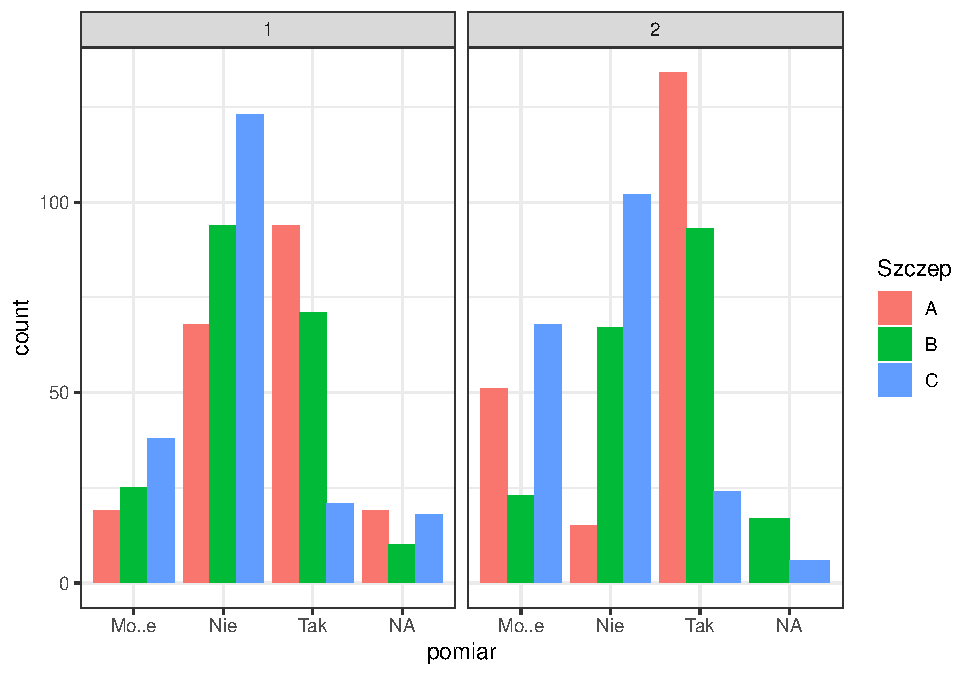
\includegraphics{_main_files/figure-latex/unnamed-chunk-37-1.pdf}

Dla histogramu najważniejszy parametr to \texttt{binwidth} określający szerokość ``słupków''.

Możemy też wybrać czy chcemy żeby były zliczane ilości elementów (domyślnie), czy ma być pokazana gęstość rozkładu - w \texttt{aes} należy wpisać \texttt{y=..density..} albo procenty \texttt{y=((..count..)/sum(..count..))*100} (w przypadku procentów lepiej jednak policzyć je wcześniej i podać już gotowe wartości do ggplot, w bardziej skomplikowanych przypadkach ggplot może sobie nie poradzić). Do dodania znaków \% potrzebna jest zmiana parametrów osi, o tym później.

Można też zmienić kolor wypełnienia słupków - \texttt{fill} lub kolor linii - color.

\begin{Shaded}
\begin{Highlighting}[]
\NormalTok{p }\SpecialCharTok{+} \FunctionTok{geom\_histogram}\NormalTok{(}\AttributeTok{binwidth =} \FloatTok{0.5}\NormalTok{)}
\end{Highlighting}
\end{Shaded}

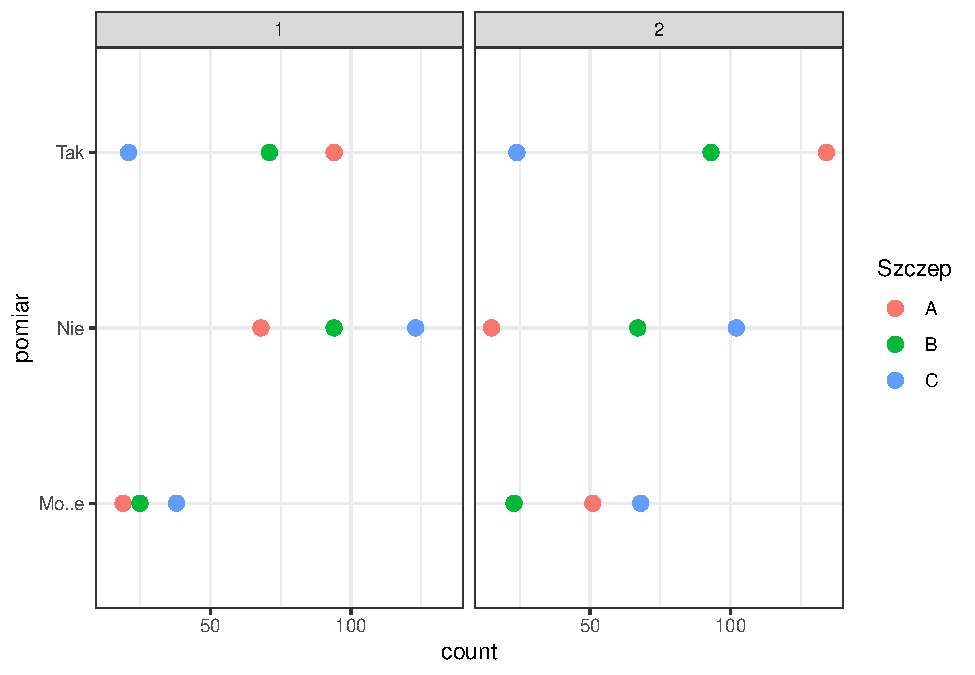
\includegraphics{_main_files/figure-latex/unnamed-chunk-38-1.pdf}

\begin{Shaded}
\begin{Highlighting}[]
\CommentTok{\# Histogram z gęstością na osi Y}
\NormalTok{p }\SpecialCharTok{+} \FunctionTok{geom\_histogram}\NormalTok{(}\AttributeTok{binwidth =} \FloatTok{0.5}\NormalTok{, }\FunctionTok{aes}\NormalTok{(}\AttributeTok{y =}\NormalTok{ ..density..))}
\end{Highlighting}
\end{Shaded}

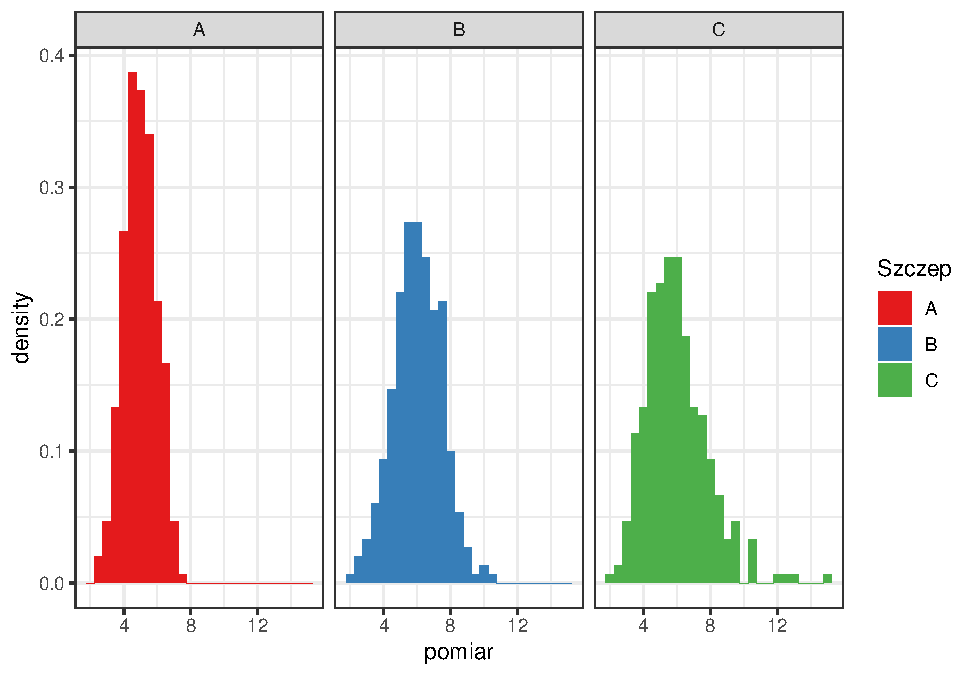
\includegraphics{_main_files/figure-latex/unnamed-chunk-38-2.pdf}

\begin{Shaded}
\begin{Highlighting}[]
\CommentTok{\# Histogram z wartością \% na osi Y}
\NormalTok{p }\SpecialCharTok{+} \FunctionTok{geom\_histogram}\NormalTok{(}\AttributeTok{binwidth =} \FloatTok{0.5}\NormalTok{, }\FunctionTok{aes}\NormalTok{(}\AttributeTok{y =}\NormalTok{ ((..count..)}\SpecialCharTok{/}\FunctionTok{sum}\NormalTok{(..count..)}\SpecialCharTok{*}\DecValTok{100}\NormalTok{)))}
\end{Highlighting}
\end{Shaded}

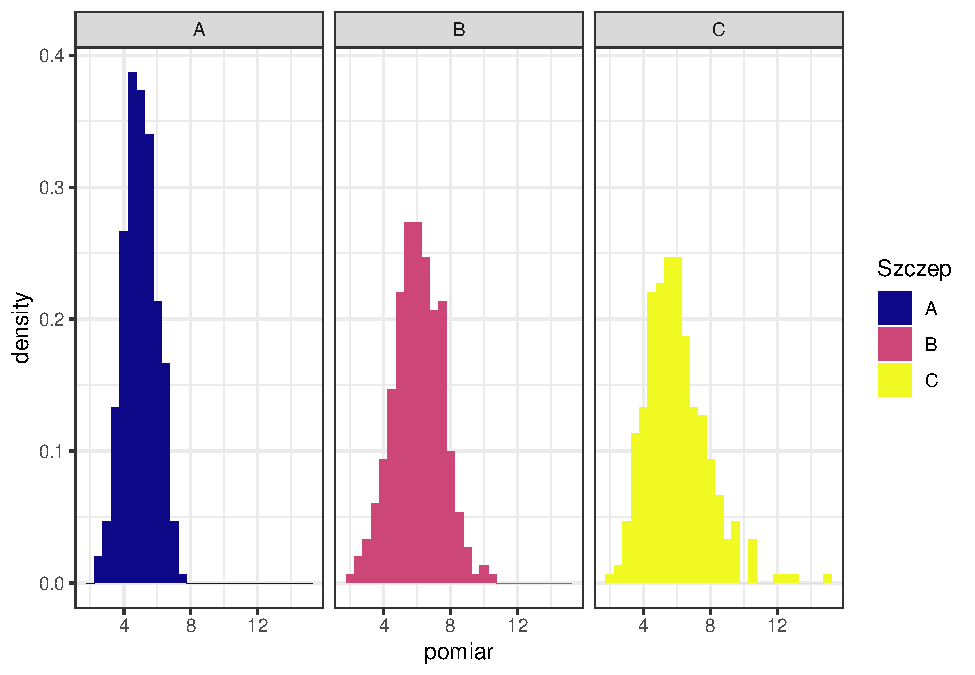
\includegraphics{_main_files/figure-latex/unnamed-chunk-38-3.pdf}

\begin{Shaded}
\begin{Highlighting}[]
\CommentTok{\# Zmiana koloru wypełnienia histogramu}
\NormalTok{p }\SpecialCharTok{+} \FunctionTok{geom\_histogram}\NormalTok{(}\AttributeTok{binwidth =} \FloatTok{0.5}\NormalTok{, }\FunctionTok{aes}\NormalTok{(}\AttributeTok{y =}\NormalTok{ ..density..), }
                   \AttributeTok{fill =} \StringTok{"lightgreen"}\NormalTok{, }\AttributeTok{color =} \StringTok{"black"}\NormalTok{)}
\end{Highlighting}
\end{Shaded}

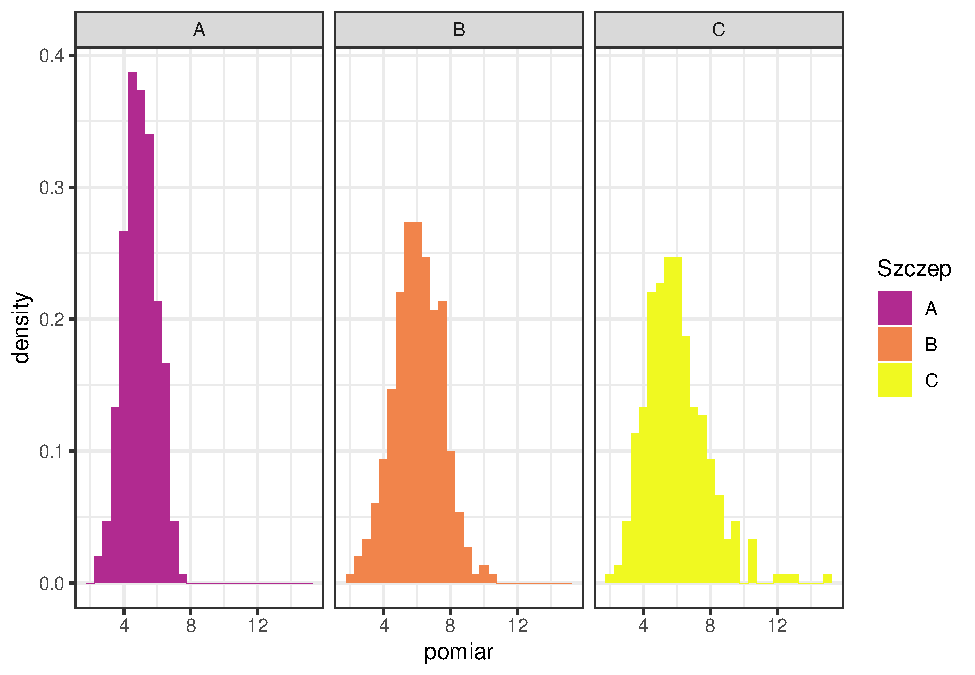
\includegraphics{_main_files/figure-latex/unnamed-chunk-38-4.pdf}

\begin{Shaded}
\begin{Highlighting}[]
\CommentTok{\# Dodanie wszystkich obserwacji do wykresu {-} geom\_rug()}
\NormalTok{p }\SpecialCharTok{+} \FunctionTok{geom\_histogram}\NormalTok{(}\AttributeTok{binwidth =} \FloatTok{0.5}\NormalTok{, }\FunctionTok{aes}\NormalTok{(}\AttributeTok{y =}\NormalTok{ ..density..), }
                   \AttributeTok{fill =} \StringTok{"lightgreen"}\NormalTok{, }\AttributeTok{color =} \StringTok{"black"}\NormalTok{)}\SpecialCharTok{+}
  \FunctionTok{geom\_rug}\NormalTok{()}
\end{Highlighting}
\end{Shaded}

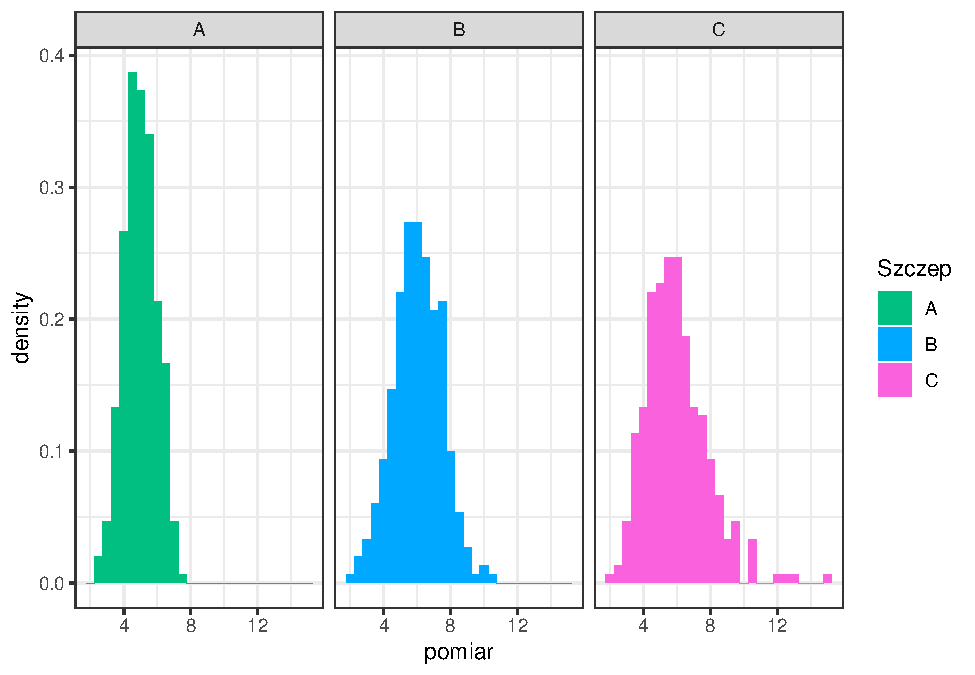
\includegraphics{_main_files/figure-latex/unnamed-chunk-38-5.pdf}

Histogram możemy łatwo zmienić na \texttt{geom\_density} (gęstość) albo połączyć oba na jednym wykresie (należy pamiętać żeby ujednolicić oś Y - w histogramie ustawić \texttt{y=..density..} albo w density \texttt{y\ =\ ..count..})

Wykresy gęstości są dużo czytelniejsze od histogramów przy większej liczbie grup/kolorów na wykresie.

\begin{Shaded}
\begin{Highlighting}[]
\NormalTok{p }\SpecialCharTok{+} \FunctionTok{geom\_density}\NormalTok{()}
\end{Highlighting}
\end{Shaded}

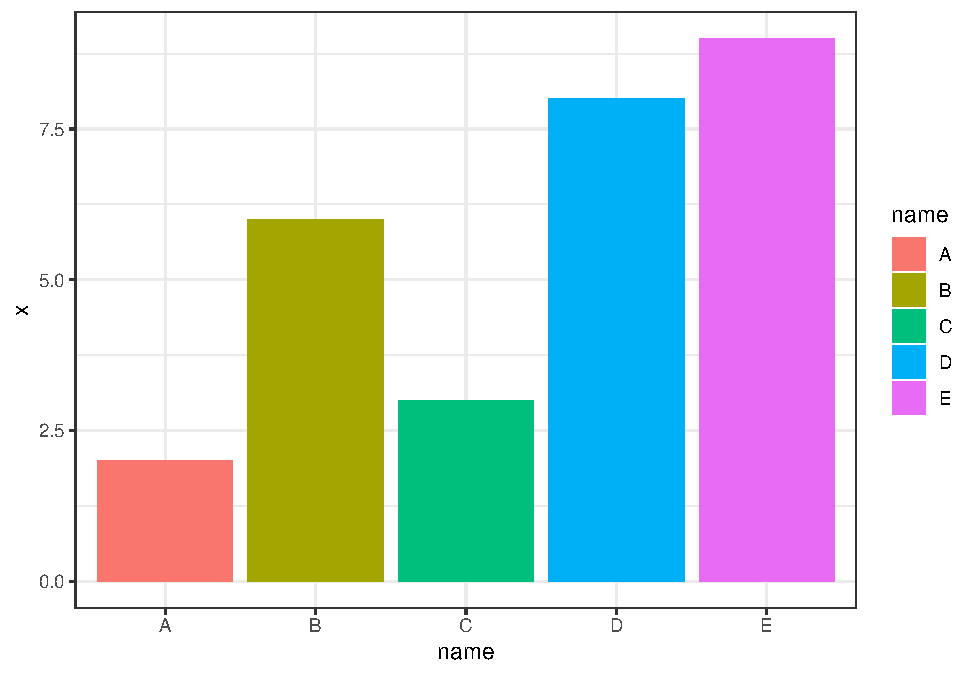
\includegraphics{_main_files/figure-latex/unnamed-chunk-39-1.pdf}

\begin{Shaded}
\begin{Highlighting}[]
\CommentTok{\# Wykres łączący histogram i gęstość}
\NormalTok{p }\SpecialCharTok{+} \FunctionTok{geom\_histogram}\NormalTok{(}\AttributeTok{binwidth =} \FloatTok{0.5}\NormalTok{, }\FunctionTok{aes}\NormalTok{(}\AttributeTok{y =}\NormalTok{ ..density..))}\SpecialCharTok{+}
  \FunctionTok{geom\_density}\NormalTok{(}\AttributeTok{color =} \StringTok{"red"}\NormalTok{)}
\end{Highlighting}
\end{Shaded}

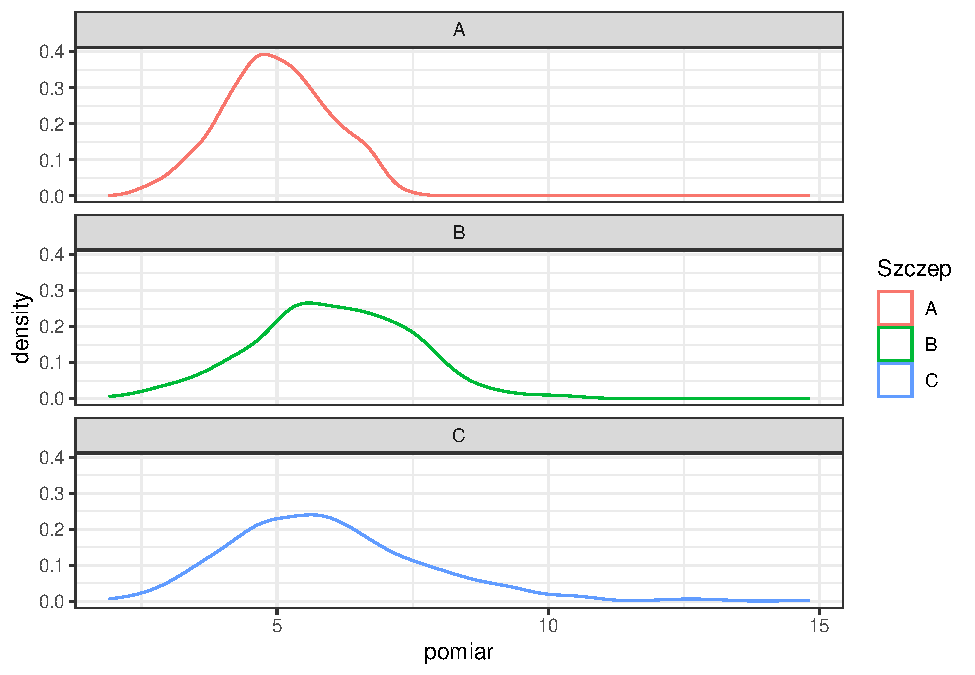
\includegraphics{_main_files/figure-latex/unnamed-chunk-39-2.pdf}

\begin{Shaded}
\begin{Highlighting}[]
\CommentTok{\# albo tak, ale wtedy trzeba count w density podzielić przez coś {-} konkretną liczbę lepiej dobrać indywidualnie do każdego wykresu}
\NormalTok{p }\SpecialCharTok{+} \FunctionTok{geom\_histogram}\NormalTok{(}\AttributeTok{binwidth =} \FloatTok{0.5}\NormalTok{)}\SpecialCharTok{+}
  \FunctionTok{geom\_density}\NormalTok{(}\AttributeTok{color =} \StringTok{"red"}\NormalTok{, }\FunctionTok{aes}\NormalTok{(}\AttributeTok{y =}\NormalTok{ ..count..}\SpecialCharTok{/}\DecValTok{2}\NormalTok{))}
\end{Highlighting}
\end{Shaded}

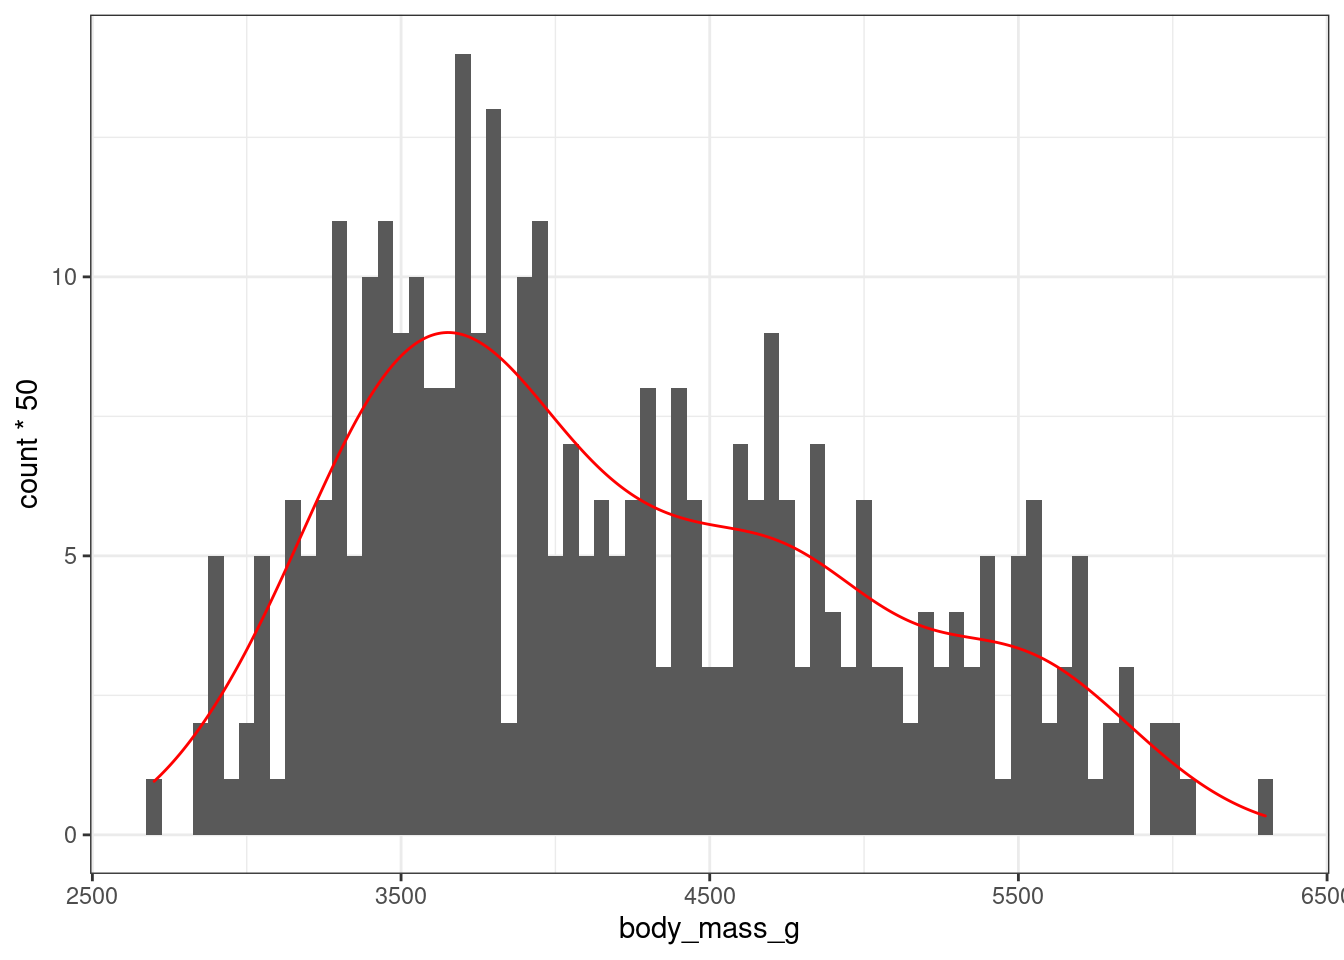
\includegraphics{_main_files/figure-latex/unnamed-chunk-39-3.pdf}

\begin{Shaded}
\begin{Highlighting}[]
\CommentTok{\# Zamiast density można też użyć geom\_freqpoly, który da bardziej "kanciasty" wykres}
\CommentTok{\# Wymaga parametru binwidth tak samo jak histogram}
\NormalTok{p }\SpecialCharTok{+} \FunctionTok{geom\_freqpoly}\NormalTok{(}\AttributeTok{binwidth =} \FloatTok{0.5}\NormalTok{)}
\end{Highlighting}
\end{Shaded}

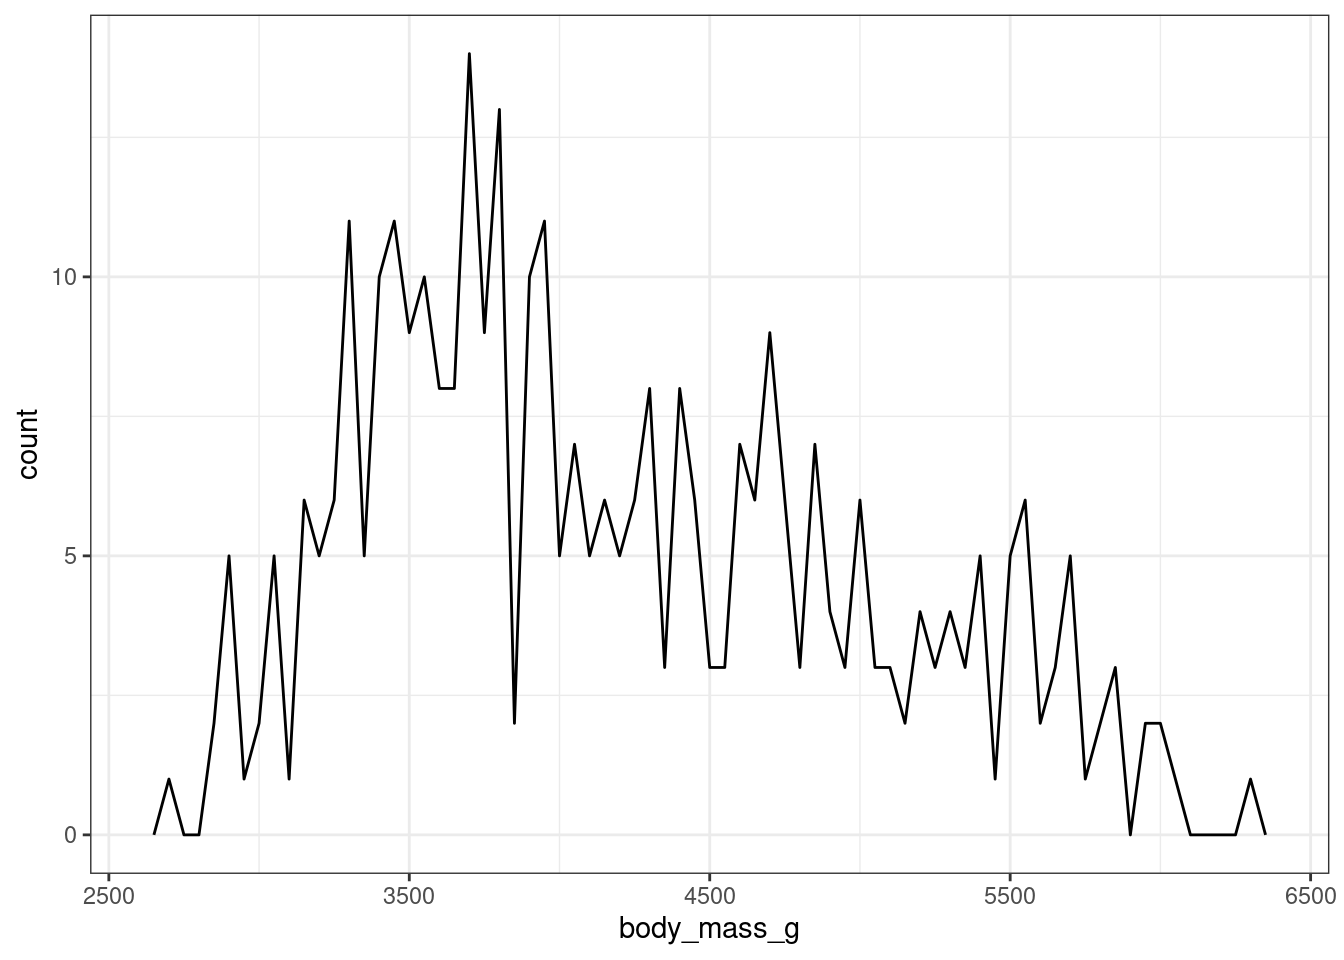
\includegraphics{_main_files/figure-latex/unnamed-chunk-39-4.pdf}

\hypertarget{wykres-pudeux142kowy---boxplot}{%
\subsection{Wykres pudełkowy - boxplot}\label{wykres-pudeux142kowy---boxplot}}

Na wykresie pudełkowym linia obrazuje medianę, pudełko to przestrzeń między 1 i 3 kwantylem, wąsy to zakres danych, a wszystkie punkty to obserwacje odstające.

Zamiast histogramu możemy zrobić boxplot, w tym wypadku x to nazwa szczepu, a y to mierzona cecha. Na osi X należy zawsze umieszczać zmienną jakościową, a na osi Y zmienną ilościową

\begin{Shaded}
\begin{Highlighting}[]
\CommentTok{\# pojedynczy boxplot}
\NormalTok{p }\OtherTok{\textless{}{-}} \FunctionTok{ggplot}\NormalTok{(}\AttributeTok{data =}\NormalTok{ dane1\_1, }\FunctionTok{aes}\NormalTok{(}\AttributeTok{x =} \StringTok{"Szczep A"}\NormalTok{, }\AttributeTok{y =}\NormalTok{ pomiar))}
\NormalTok{p }\SpecialCharTok{+} \FunctionTok{geom\_boxplot}\NormalTok{()}
\end{Highlighting}
\end{Shaded}

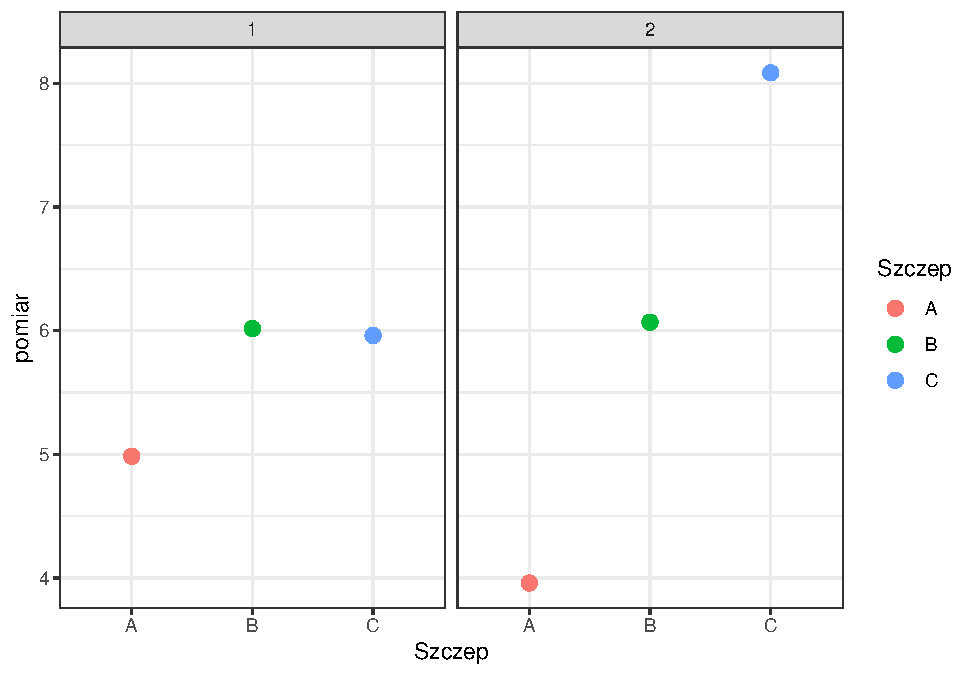
\includegraphics{_main_files/figure-latex/unnamed-chunk-40-1.pdf}

\begin{Shaded}
\begin{Highlighting}[]
\CommentTok{\# boxplot dla każdej kategorii}
\NormalTok{p }\OtherTok{\textless{}{-}} \FunctionTok{ggplot}\NormalTok{(}\AttributeTok{data =}\NormalTok{ dane1, }\FunctionTok{aes}\NormalTok{(}\AttributeTok{x =}\NormalTok{ Szczep, }\AttributeTok{y =}\NormalTok{ pomiar))}
\NormalTok{p }\SpecialCharTok{+} \FunctionTok{geom\_boxplot}\NormalTok{()}
\end{Highlighting}
\end{Shaded}

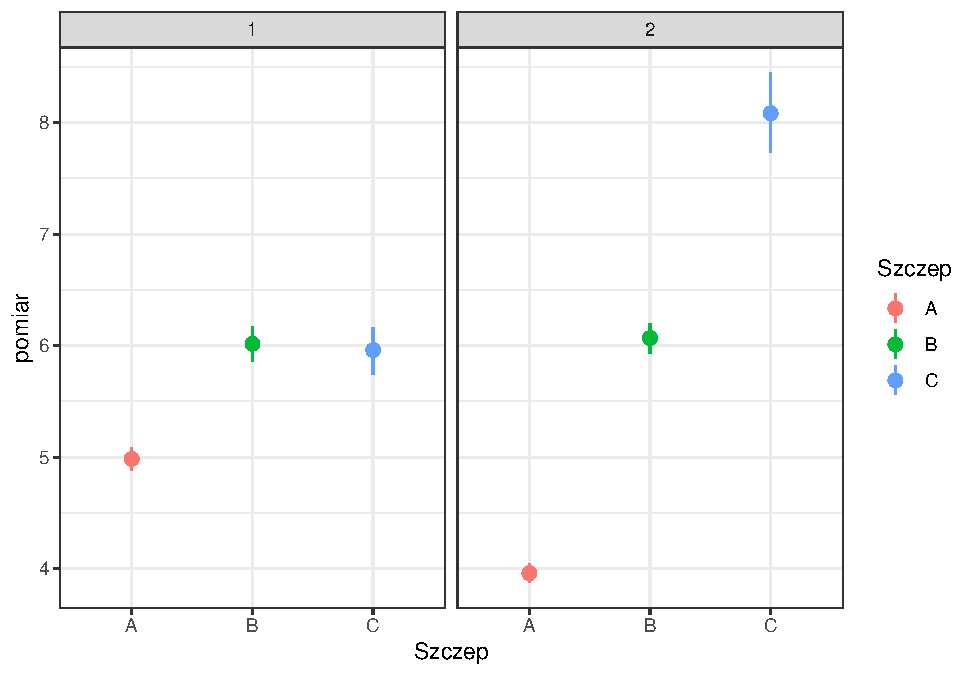
\includegraphics{_main_files/figure-latex/unnamed-chunk-40-2.pdf}

\begin{Shaded}
\begin{Highlighting}[]
\CommentTok{\# do boxplota można dodać wcięcia, jeżeli wcięcia dwóch boxplotów na siebie nie zachodzą }
\CommentTok{\# można uznać że mediany tych dwóch grup są od siebie znacząco różne}
\NormalTok{p }\SpecialCharTok{+} \FunctionTok{geom\_boxplot}\NormalTok{(}\AttributeTok{notch =} \ConstantTok{TRUE}\NormalTok{)}
\end{Highlighting}
\end{Shaded}

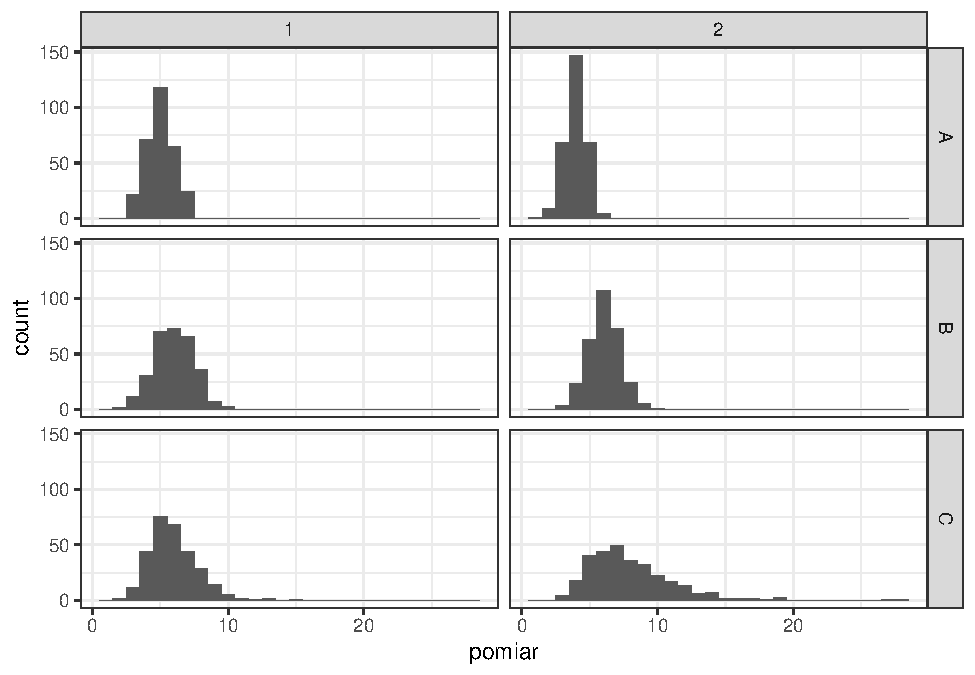
\includegraphics{_main_files/figure-latex/unnamed-chunk-40-3.pdf}

\hypertarget{wykres-skrzypcowy}{%
\subsection{Wykres skrzypcowy}\label{wykres-skrzypcowy}}

Odmianą boxplotów są tzw. wykresy skrzypcowe, które pozwalają też na pokazanie kształtu rozkładu - pozwala to np. na wykrycie rozkładu, który ma dwa maksima. W ggplot2 można je wygenerować funkcją \texttt{geom\_violin}.

\begin{Shaded}
\begin{Highlighting}[]
\NormalTok{p }\OtherTok{\textless{}{-}} \FunctionTok{ggplot}\NormalTok{(}\AttributeTok{data=}\NormalTok{dane1, }\FunctionTok{aes}\NormalTok{(}\AttributeTok{x =}\NormalTok{ Szczep, }\AttributeTok{y =}\NormalTok{ pomiar))}
\NormalTok{p }\SpecialCharTok{+} \FunctionTok{geom\_violin}\NormalTok{(}\FunctionTok{aes}\NormalTok{(}\AttributeTok{color =} \FunctionTok{factor}\NormalTok{(warunki)))}
\end{Highlighting}
\end{Shaded}

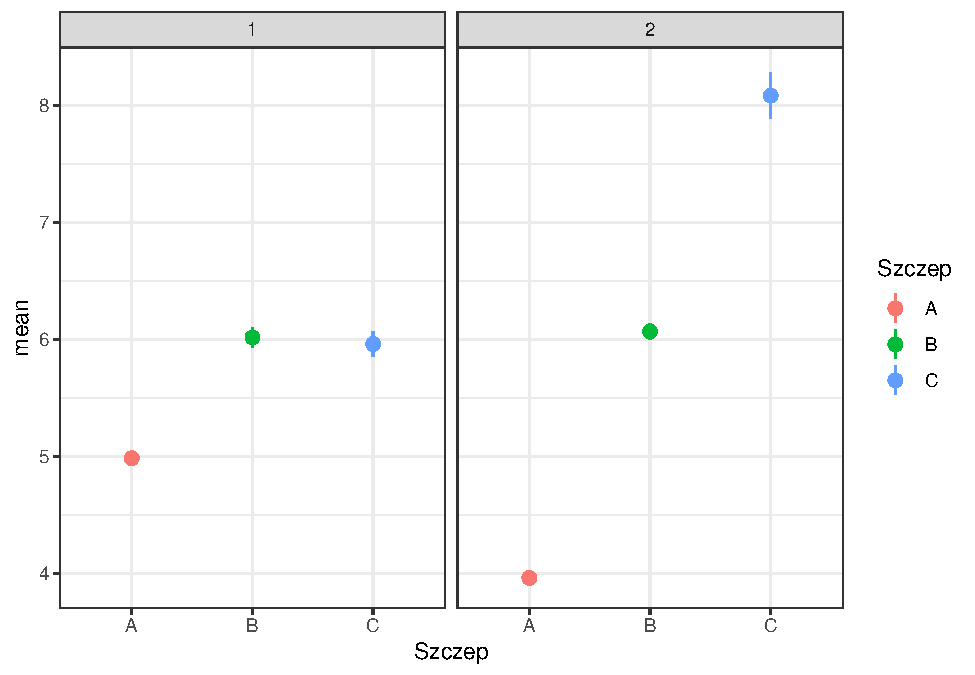
\includegraphics{_main_files/figure-latex/unnamed-chunk-41-1.pdf}

\begin{Shaded}
\begin{Highlighting}[]
\CommentTok{\# przykładowe dane}
\NormalTok{dane }\OtherTok{\textless{}{-}} \FunctionTok{data.frame}\NormalTok{(}\AttributeTok{x =} \FunctionTok{c}\NormalTok{(}\FunctionTok{rnorm}\NormalTok{(}\DecValTok{100}\NormalTok{), }\FunctionTok{rnorm}\NormalTok{(}\DecValTok{100}\NormalTok{, }\DecValTok{3}\NormalTok{), }\FunctionTok{rnorm}\NormalTok{(}\DecValTok{100}\NormalTok{, }\DecValTok{1}\NormalTok{), }\FunctionTok{rnorm}\NormalTok{(}\DecValTok{100}\NormalTok{, }\DecValTok{5}\NormalTok{)), }
                   \AttributeTok{faktor =} \FunctionTok{rep}\NormalTok{(}\FunctionTok{c}\NormalTok{(}\StringTok{"A"}\NormalTok{, }\StringTok{"B"}\NormalTok{), }\AttributeTok{each =} \DecValTok{200}\NormalTok{))}

\NormalTok{p }\OtherTok{\textless{}{-}} \FunctionTok{ggplot}\NormalTok{(}\AttributeTok{data =}\NormalTok{ dane, }\FunctionTok{aes}\NormalTok{(}\AttributeTok{y =}\NormalTok{ x, }\AttributeTok{x =}\NormalTok{ faktor, }\AttributeTok{fill =}\NormalTok{ faktor))}
\NormalTok{p }\SpecialCharTok{+} \FunctionTok{geom\_violin}\NormalTok{()}
\end{Highlighting}
\end{Shaded}

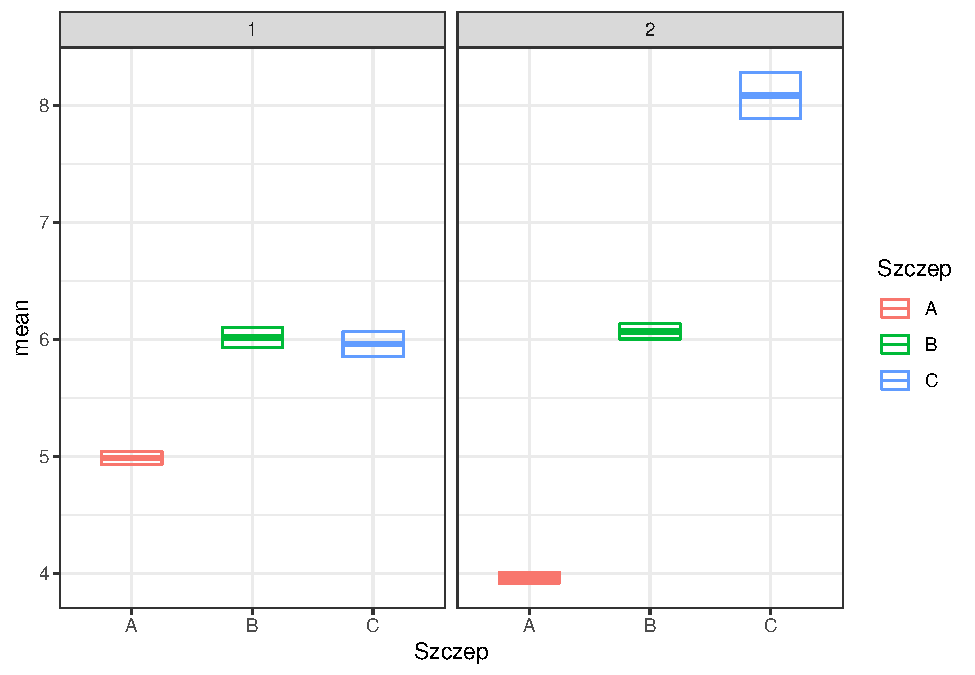
\includegraphics{_main_files/figure-latex/unnamed-chunk-41-2.pdf}

\begin{Shaded}
\begin{Highlighting}[]
\CommentTok{\# nie przyciety wykres}
\NormalTok{p }\SpecialCharTok{+} \FunctionTok{geom\_violin}\NormalTok{(}\AttributeTok{trim=}\ConstantTok{FALSE}\NormalTok{)}
\end{Highlighting}
\end{Shaded}

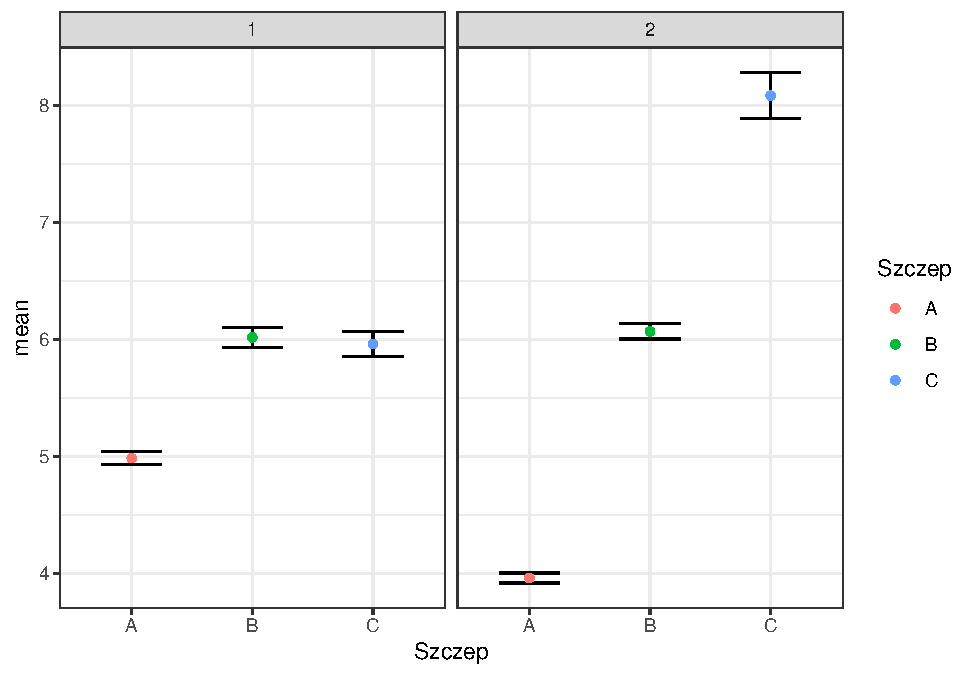
\includegraphics{_main_files/figure-latex/unnamed-chunk-41-3.pdf}

\hypertarget{dodanie-wszystkich-obserwacji-do-boxplotviolin}{%
\subsection{Dodanie wszystkich obserwacji do boxplot/violin}\label{dodanie-wszystkich-obserwacji-do-boxplotviolin}}

Dobrą praktyką jest przy używaniu wykresów pudełkowych lub skrzypcowych pokazanie wszystkich uzyskanych obserwacji (o ile nie ma ich za dużo). Można w tym celu użyć funkcji \texttt{geom\_jitter} albo ładniejszych \texttt{geom\_beeswarm} i \texttt{geom\_quasirandom} z pakietu ggbeeswarm.

Przy pomocy argumentu alpha można kontrolować przezroczystość punktów - przydatne gdy jest ich dużo.

\begin{Shaded}
\begin{Highlighting}[]
\NormalTok{dane1\_2 }\OtherTok{\textless{}{-}}\NormalTok{ dane1 }\SpecialCharTok{\%\textgreater{}\%} \FunctionTok{filter}\NormalTok{(warunki }\SpecialCharTok{==} \DecValTok{1}\NormalTok{)}

\CommentTok{\# Boxplot dla każdego szczepu}
\NormalTok{p }\OtherTok{\textless{}{-}} \FunctionTok{ggplot}\NormalTok{(}\AttributeTok{data =}\NormalTok{ dane1\_2, }\FunctionTok{aes}\NormalTok{(}\AttributeTok{x =}\NormalTok{ Szczep, }\AttributeTok{y =}\NormalTok{ pomiar))}
\NormalTok{p }\SpecialCharTok{+} \FunctionTok{geom\_boxplot}\NormalTok{(}\FunctionTok{aes}\NormalTok{(}\AttributeTok{color =}\NormalTok{ Szczep))}\SpecialCharTok{+}
  \FunctionTok{geom\_jitter}\NormalTok{(}\FunctionTok{aes}\NormalTok{(}\AttributeTok{color =}\NormalTok{ Szczep), }\AttributeTok{alpha =} \FloatTok{0.2}\NormalTok{)}
\end{Highlighting}
\end{Shaded}

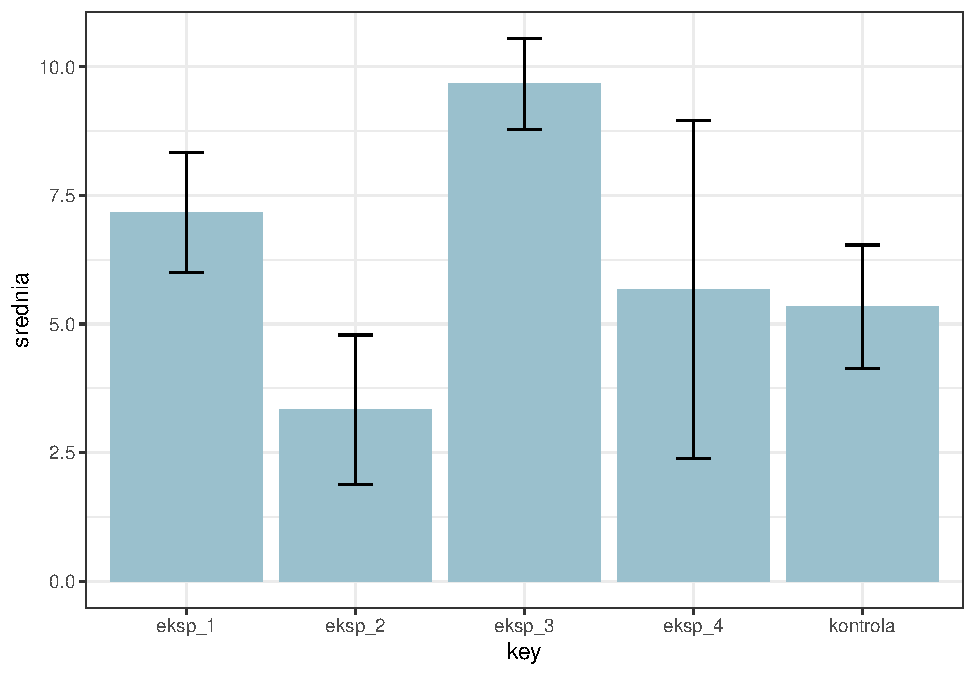
\includegraphics{_main_files/figure-latex/unnamed-chunk-42-1.pdf}

\begin{Shaded}
\begin{Highlighting}[]
\CommentTok{\# usuwamy punkty pochodzące od boxplota}
\NormalTok{p }\SpecialCharTok{+} \FunctionTok{geom\_boxplot}\NormalTok{(}\FunctionTok{aes}\NormalTok{(}\AttributeTok{color =}\NormalTok{ Szczep), }\AttributeTok{outlier.alpha =} \DecValTok{0}\NormalTok{)}\SpecialCharTok{+}
  \FunctionTok{geom\_jitter}\NormalTok{(}\FunctionTok{aes}\NormalTok{(}\AttributeTok{color =}\NormalTok{ Szczep), }\AttributeTok{alpha =} \FloatTok{0.2}\NormalTok{)}
\end{Highlighting}
\end{Shaded}

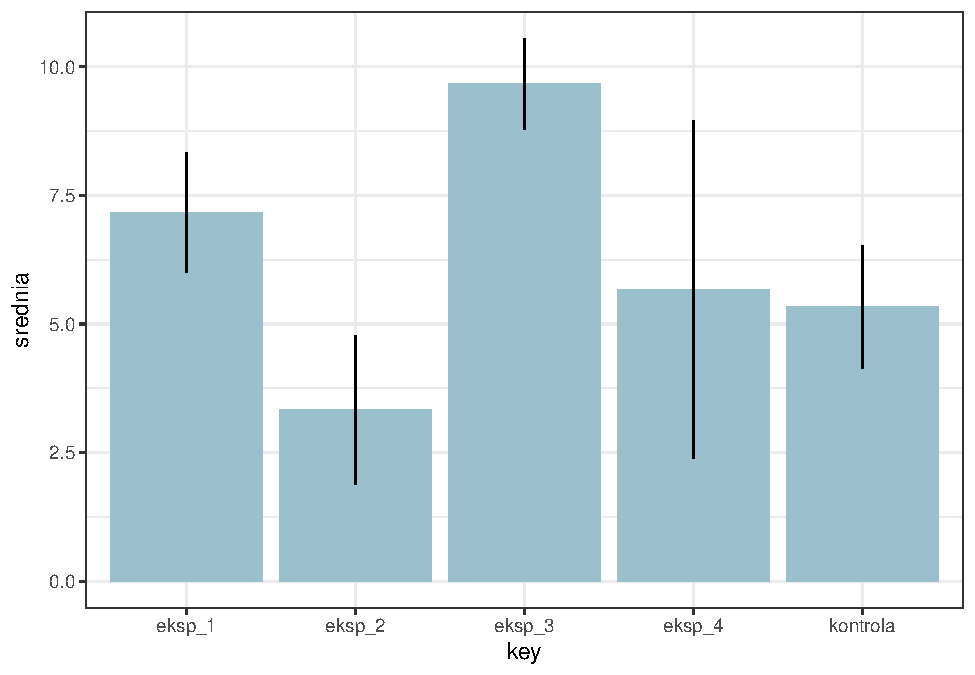
\includegraphics{_main_files/figure-latex/unnamed-chunk-42-2.pdf}

\begin{Shaded}
\begin{Highlighting}[]
\CommentTok{\# beeswarm}
\FunctionTok{library}\NormalTok{(ggbeeswarm)}

\NormalTok{p }\SpecialCharTok{+} \FunctionTok{geom\_boxplot}\NormalTok{(}\FunctionTok{aes}\NormalTok{(}\AttributeTok{color =}\NormalTok{ Szczep), }\AttributeTok{outlier.alpha =} \DecValTok{0}\NormalTok{)}\SpecialCharTok{+}
  \FunctionTok{geom\_beeswarm}\NormalTok{(}\FunctionTok{aes}\NormalTok{(}\AttributeTok{color =}\NormalTok{ Szczep), }\AttributeTok{alpha =} \FloatTok{0.2}\NormalTok{)}
\end{Highlighting}
\end{Shaded}

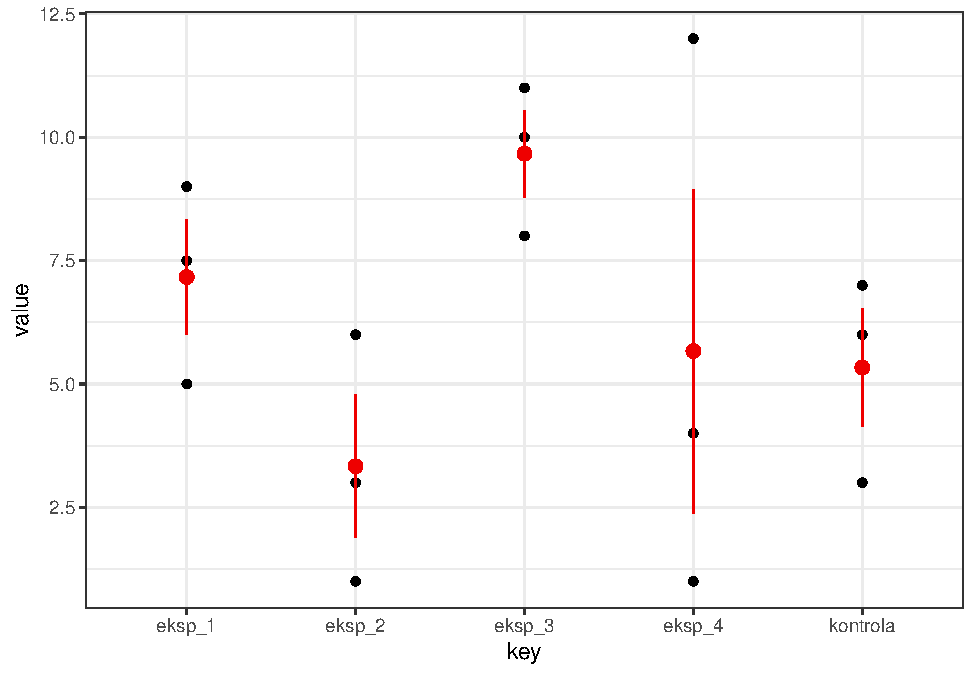
\includegraphics{_main_files/figure-latex/unnamed-chunk-42-3.pdf}

\begin{Shaded}
\begin{Highlighting}[]
\CommentTok{\# quasirandom}
\NormalTok{p }\SpecialCharTok{+} \FunctionTok{geom\_boxplot}\NormalTok{(}\FunctionTok{aes}\NormalTok{(}\AttributeTok{color =}\NormalTok{ Szczep), }\AttributeTok{outlier.alpha =} \DecValTok{0}\NormalTok{)}\SpecialCharTok{+}
  \FunctionTok{geom\_quasirandom}\NormalTok{(}\FunctionTok{aes}\NormalTok{(}\AttributeTok{color =}\NormalTok{ Szczep), }\AttributeTok{alpha =} \FloatTok{0.2}\NormalTok{)}
\end{Highlighting}
\end{Shaded}

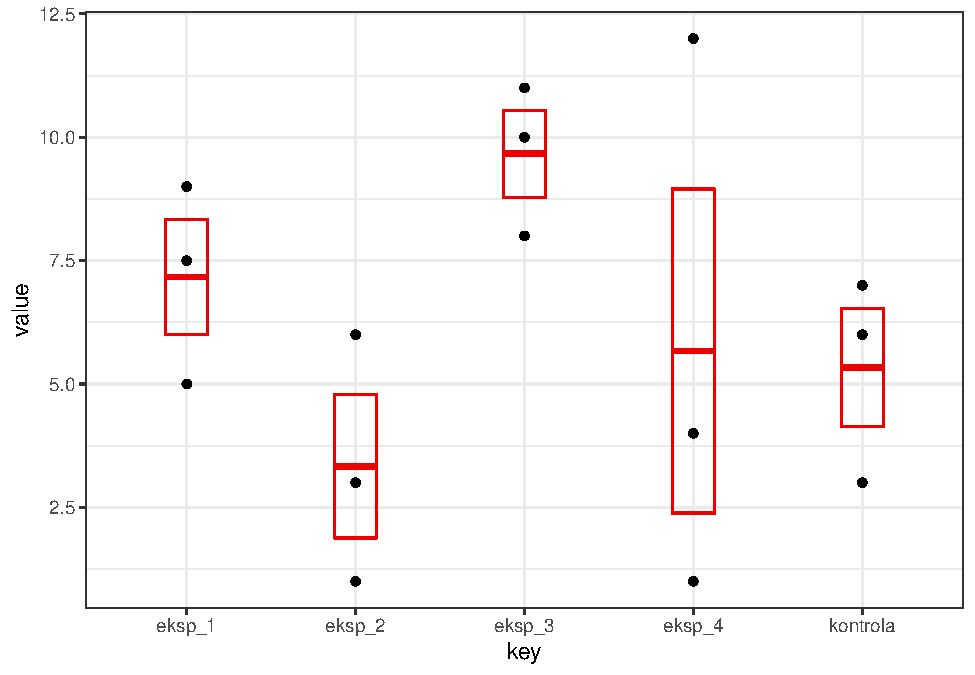
\includegraphics{_main_files/figure-latex/unnamed-chunk-42-4.pdf}

\begin{Shaded}
\begin{Highlighting}[]
\CommentTok{\# quasirandom + geom\_violin}
\NormalTok{p }\OtherTok{\textless{}{-}} \FunctionTok{ggplot}\NormalTok{(}\AttributeTok{data=}\NormalTok{dane1, }\FunctionTok{aes}\NormalTok{(}\AttributeTok{x =}\NormalTok{ Szczep, }\AttributeTok{y =}\NormalTok{ pomiar))}
\NormalTok{p }\SpecialCharTok{+} \FunctionTok{geom\_violin}\NormalTok{(}\FunctionTok{aes}\NormalTok{(}\AttributeTok{color =} \FunctionTok{factor}\NormalTok{(warunki)))}\SpecialCharTok{+}
  \FunctionTok{geom\_quasirandom}\NormalTok{(}\FunctionTok{aes}\NormalTok{(}\AttributeTok{color =} \FunctionTok{factor}\NormalTok{(warunki)), }
                   \AttributeTok{dodge.width =} \FloatTok{0.9}\NormalTok{, }\CommentTok{\# pozwala na rodział kolorów na dwie grupy}
                   \AttributeTok{alpha =} \FloatTok{0.1}\NormalTok{)}
\end{Highlighting}
\end{Shaded}

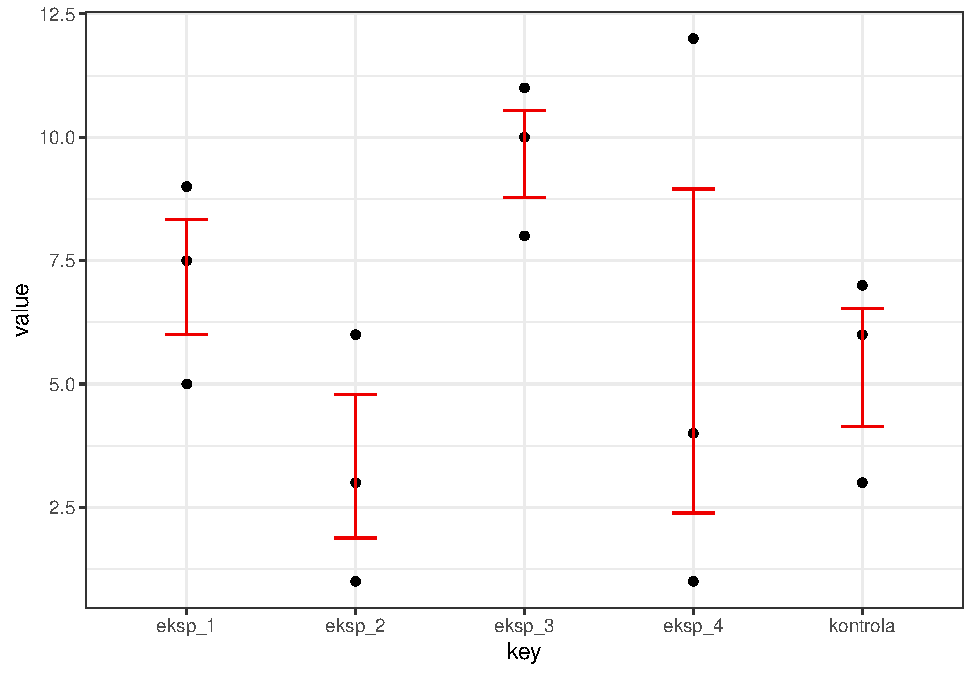
\includegraphics{_main_files/figure-latex/unnamed-chunk-42-5.pdf}

Można też połączyć wszystko w całość korzystając z dodatkowych pakietów ggdist i gghalves, na podstawie strony: \href{https://www.cedricscherer.com/2021/06/06/visualizing-distributions-with-raincloud-plots-with-ggplot2/}{visualizing-distributions-with-raincloud-plots-with-ggplot2}

\begin{Shaded}
\begin{Highlighting}[]
\FunctionTok{ggplot}\NormalTok{(dane1\_2, }\FunctionTok{aes}\NormalTok{(}\AttributeTok{x =}\NormalTok{ Szczep, }\AttributeTok{y =}\NormalTok{ pomiar, }\AttributeTok{color =}\NormalTok{ Szczep, }\AttributeTok{fill =}\NormalTok{ Szczep)) }\SpecialCharTok{+} 
\NormalTok{  ggdist}\SpecialCharTok{::}\FunctionTok{stat\_halfeye}\NormalTok{(}
    \AttributeTok{adjust =}\NormalTok{ .}\DecValTok{5}\NormalTok{, }
    \AttributeTok{width =}\NormalTok{ .}\DecValTok{6}\NormalTok{, }
    \AttributeTok{.width =} \DecValTok{0}\NormalTok{, }
    \AttributeTok{justification =} \SpecialCharTok{{-}}\NormalTok{.}\DecValTok{2}\NormalTok{, }
    \AttributeTok{point\_colour =} \ConstantTok{NA}
\NormalTok{  ) }\SpecialCharTok{+} 
  \FunctionTok{geom\_boxplot}\NormalTok{(}
    \AttributeTok{width =}\NormalTok{ .}\DecValTok{15}\NormalTok{, }
    \AttributeTok{outlier.shape =} \ConstantTok{NA}\NormalTok{,}
    \AttributeTok{alpha =} \FloatTok{0.2}
\NormalTok{  ) }\SpecialCharTok{+}
  \DocumentationTok{\#\# add justified jitter from the \{gghalves\} package}
\NormalTok{  gghalves}\SpecialCharTok{::}\FunctionTok{geom\_half\_point}\NormalTok{(}
    \DocumentationTok{\#\# draw jitter on the left}
    \AttributeTok{side =} \StringTok{"l"}\NormalTok{, }
    \DocumentationTok{\#\# control range of jitter}
    \AttributeTok{range\_scale =}\NormalTok{ .}\DecValTok{4}\NormalTok{, }
    \DocumentationTok{\#\# add some transparency}
    \AttributeTok{alpha =}\NormalTok{ .}\DecValTok{3}
\NormalTok{  ) }
\end{Highlighting}
\end{Shaded}

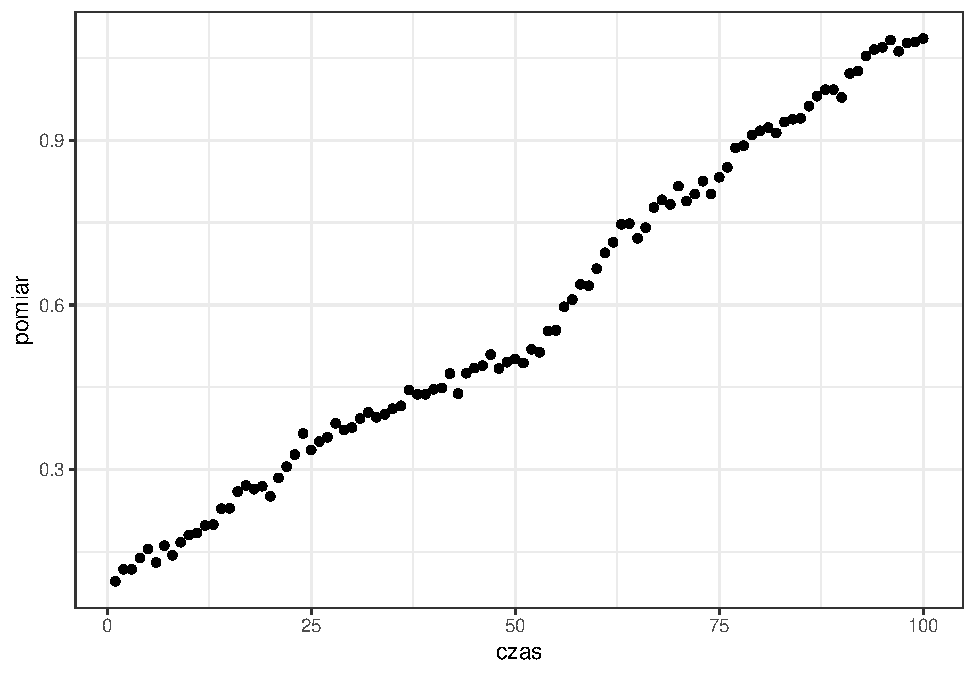
\includegraphics{_main_files/figure-latex/unnamed-chunk-43-1.pdf}

\hypertarget{dotplot}{%
\subsection{Dotplot}\label{dotplot}}

Wykres, na którym obserwacje są zaznaczane jako punkty, może być alternatywą dla histogramu albo gęstości jeżeli mamy małą liczbę danych. Punkty mogą być układane na którejś z osi albo wyśrodkowane. Podobnie jak w histogramie możemy określić parametrem \texttt{binwidth} jak mają być ułożone punkty.

\begin{Shaded}
\begin{Highlighting}[]
\NormalTok{dane\_dot }\OtherTok{\textless{}{-}} \FunctionTok{data.frame}\NormalTok{(}\AttributeTok{pomiar =} \FunctionTok{c}\NormalTok{(}\FunctionTok{rnorm}\NormalTok{(}\DecValTok{20}\NormalTok{), }\FunctionTok{rlnorm}\NormalTok{(}\DecValTok{20}\NormalTok{), }\FunctionTok{runif}\NormalTok{(}\DecValTok{20}\NormalTok{)), }
                       \AttributeTok{kategoria =} \FunctionTok{rep}\NormalTok{(}\FunctionTok{c}\NormalTok{(}\StringTok{"A"}\NormalTok{,}\StringTok{"B"}\NormalTok{,}\StringTok{"C"}\NormalTok{), }\AttributeTok{each =} \DecValTok{20}\NormalTok{))}

\NormalTok{p }\OtherTok{\textless{}{-}} \FunctionTok{ggplot}\NormalTok{(dane\_dot)}

\NormalTok{p }\SpecialCharTok{+} \FunctionTok{geom\_dotplot}\NormalTok{(}\FunctionTok{aes}\NormalTok{(}\AttributeTok{x =}\NormalTok{ pomiar))}
\end{Highlighting}
\end{Shaded}

\begin{verbatim}
## Bin width defaults to 1/30 of the range of the data. Pick better value with `binwidth`.
\end{verbatim}

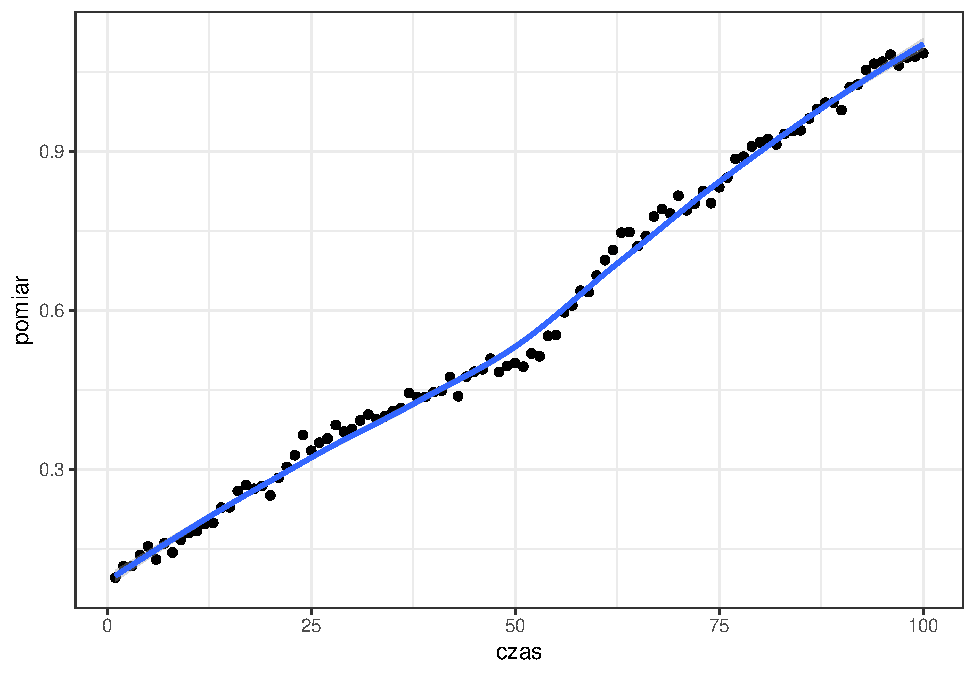
\includegraphics{_main_files/figure-latex/unnamed-chunk-44-1.pdf}

\begin{Shaded}
\begin{Highlighting}[]
\NormalTok{p }\SpecialCharTok{+} \FunctionTok{geom\_dotplot}\NormalTok{(}\FunctionTok{aes}\NormalTok{(}\AttributeTok{x =}\NormalTok{ pomiar), }\AttributeTok{binwidth =} \FloatTok{0.25}\NormalTok{)}
\end{Highlighting}
\end{Shaded}

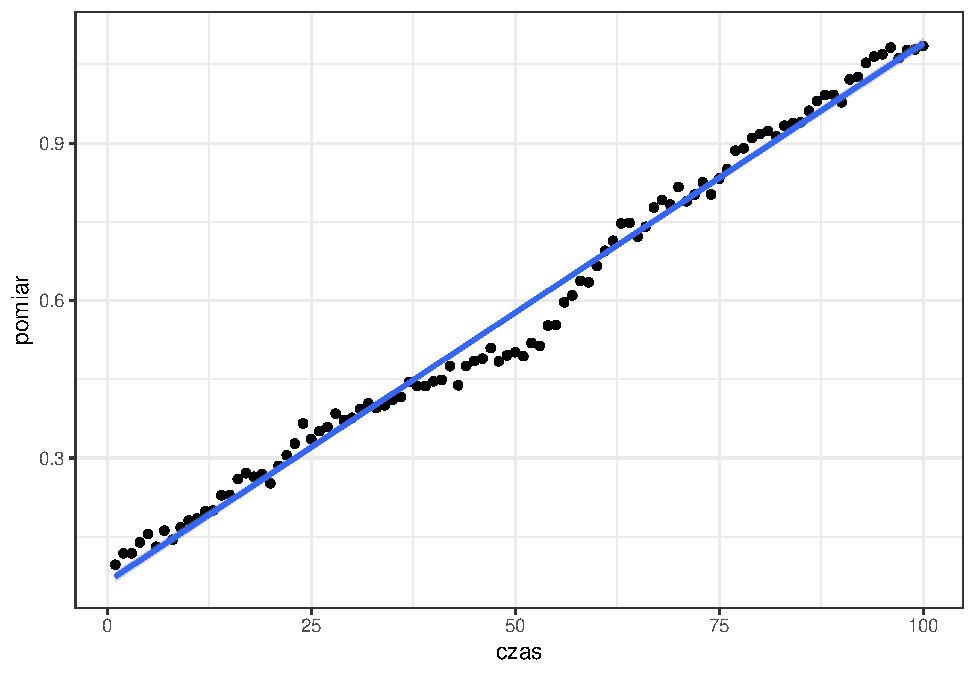
\includegraphics{_main_files/figure-latex/unnamed-chunk-44-2.pdf}

\begin{Shaded}
\begin{Highlighting}[]
\CommentTok{\# możemy kropki pokolorować według kategorii, }
\CommentTok{\# konieczne parametry stackgroups=TRUE i binpositions="all"}

\NormalTok{p }\SpecialCharTok{+} \FunctionTok{geom\_dotplot}\NormalTok{(}\FunctionTok{aes}\NormalTok{(}\AttributeTok{x =}\NormalTok{ pomiar, }\AttributeTok{fill =}\NormalTok{ kategoria), }\AttributeTok{binpositions =} \StringTok{"all"}\NormalTok{, }\AttributeTok{stackgroups =} \ConstantTok{TRUE}\NormalTok{)}
\end{Highlighting}
\end{Shaded}

\begin{verbatim}
## Bin width defaults to 1/30 of the range of the data. Pick better value with `binwidth`.
\end{verbatim}

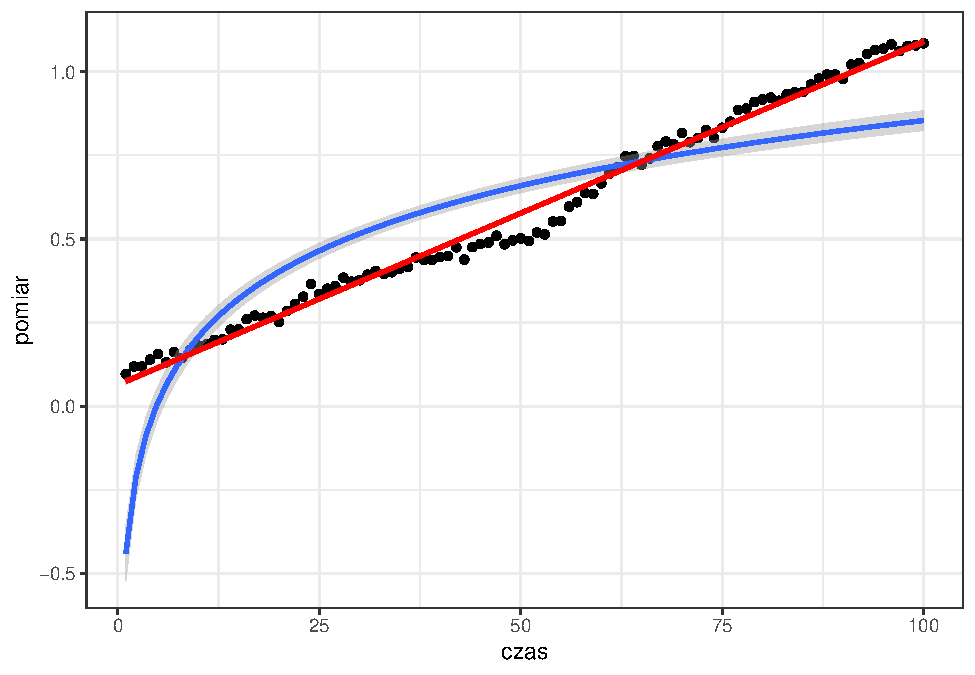
\includegraphics{_main_files/figure-latex/unnamed-chunk-44-3.pdf}

\begin{Shaded}
\begin{Highlighting}[]
\CommentTok{\# albo przedstawić każdą kategorię osobno, binaxis określa w jakim kierunku układać kropki,}
\CommentTok{\# stackdir czy mają być wyśrodkowane {-} center lub centerwhole}

\NormalTok{p }\SpecialCharTok{+} \FunctionTok{geom\_dotplot}\NormalTok{(}\FunctionTok{aes}\NormalTok{(}\AttributeTok{y =}\NormalTok{ pomiar, }\AttributeTok{x =}\NormalTok{ kategoria), }\AttributeTok{stackdir =} \StringTok{"center"}\NormalTok{, }\AttributeTok{binaxis =} \StringTok{"y"}\NormalTok{, }\AttributeTok{binwidth =} \FloatTok{0.2}\NormalTok{)}
\end{Highlighting}
\end{Shaded}

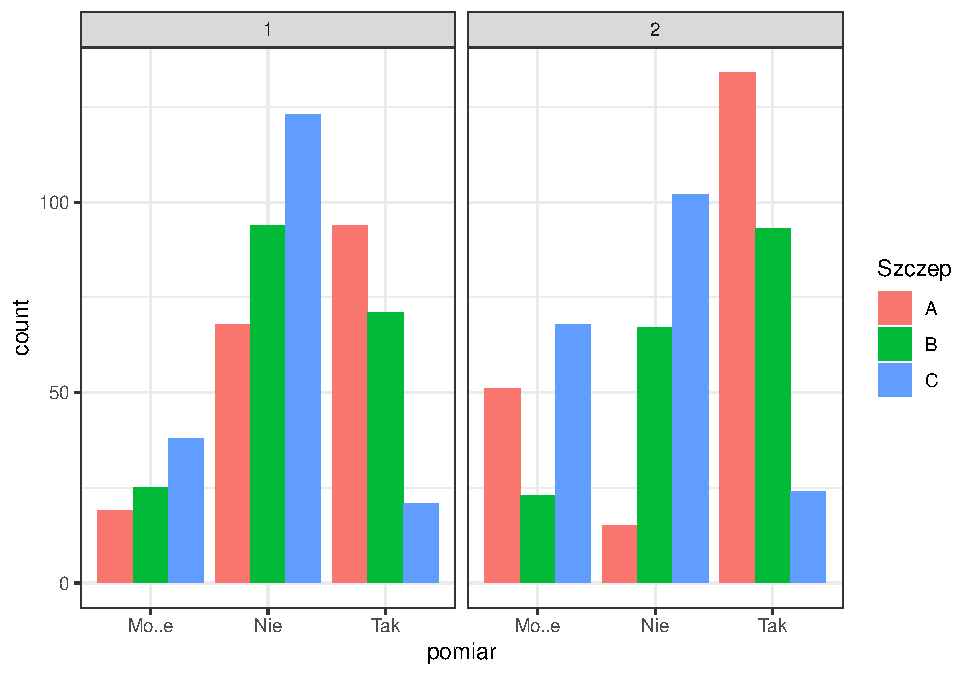
\includegraphics{_main_files/figure-latex/unnamed-chunk-44-4.pdf}

\begin{Shaded}
\begin{Highlighting}[]
\CommentTok{\# zmiana wielkości kropki przez dotsize}

\NormalTok{p }\SpecialCharTok{+} \FunctionTok{geom\_dotplot}\NormalTok{(}\FunctionTok{aes}\NormalTok{(}\AttributeTok{y =}\NormalTok{ pomiar, }\AttributeTok{x =}\NormalTok{ kategoria), }\AttributeTok{stackdir =} \StringTok{"center"}\NormalTok{, }\AttributeTok{binaxis =} \StringTok{"y"}\NormalTok{, }
                 \AttributeTok{binwidth =} \FloatTok{0.2}\NormalTok{, }\AttributeTok{dotsize =} \FloatTok{0.75}\NormalTok{)}
\end{Highlighting}
\end{Shaded}

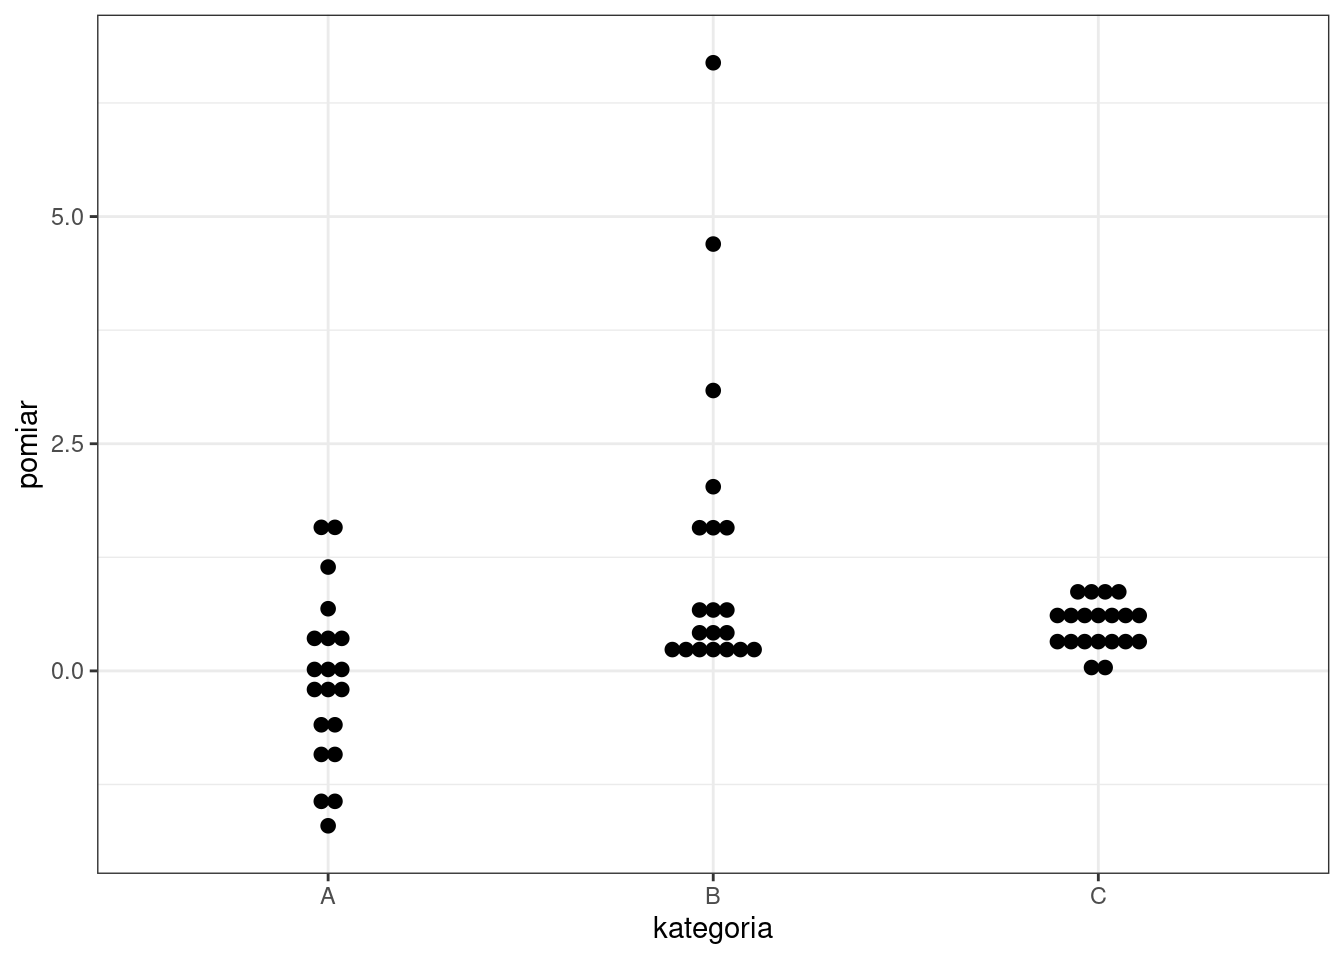
\includegraphics{_main_files/figure-latex/unnamed-chunk-44-5.pdf}

\begin{Shaded}
\begin{Highlighting}[]
\CommentTok{\# można też wybrać metodę układania kropek, domyślnie wedle gęstości, }
\CommentTok{\# podobnie jak histogram {-} method="histodot"}

\NormalTok{p }\SpecialCharTok{+} \FunctionTok{geom\_dotplot}\NormalTok{(}\FunctionTok{aes}\NormalTok{(}\AttributeTok{y =}\NormalTok{ pomiar, }\AttributeTok{x =}\NormalTok{ kategoria), }\AttributeTok{stackdir =} \StringTok{"center"}\NormalTok{, }\AttributeTok{binaxis =} \StringTok{"y"}\NormalTok{, }
                 \AttributeTok{binwidth =} \FloatTok{0.2}\NormalTok{, }\AttributeTok{dotsize =} \FloatTok{0.75}\NormalTok{, }\AttributeTok{method =} \StringTok{"histodot"}\NormalTok{)}
\end{Highlighting}
\end{Shaded}

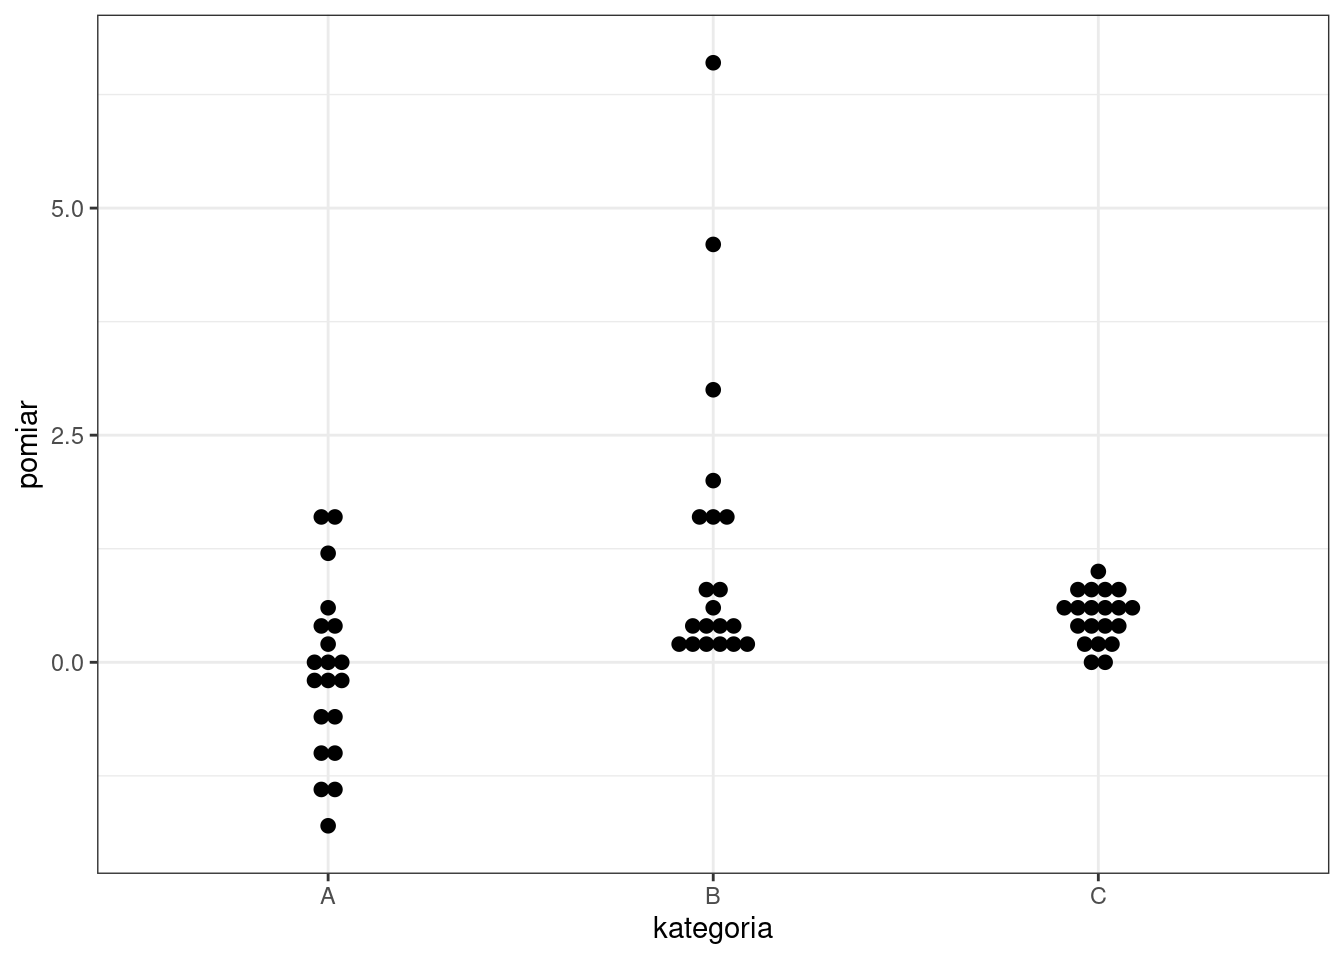
\includegraphics{_main_files/figure-latex/unnamed-chunk-44-6.pdf}

\hypertarget{barplot---wykres-sux142upkowy}{%
\section{Barplot - wykres słupkowy}\label{barplot---wykres-sux142upkowy}}

Szybkie zliczenie elementów w poszczególnych grupach możemy wykonać stosując funkcję \texttt{table}. Wystarczy podać jej kolumnę z danymi oraz kolumny zawierające wektory według których dane mają zostać podzielone na grupy. Wynikiem \texttt{table} nie jest ramka danych, więc bez przekształcenia nie można go użyć do przygotowania wykresu ggplot.

\begin{Shaded}
\begin{Highlighting}[]
\FunctionTok{table}\NormalTok{(dane2}\SpecialCharTok{$}\NormalTok{pomiar)}
\end{Highlighting}
\end{Shaded}

\begin{verbatim}
## 
## Może  Nie  Tak 
##  224  469  437
\end{verbatim}

\begin{Shaded}
\begin{Highlighting}[]
\FunctionTok{table}\NormalTok{(dane2}\SpecialCharTok{$}\NormalTok{pomiar, dane2}\SpecialCharTok{$}\NormalTok{Szczep, dane2}\SpecialCharTok{$}\NormalTok{warunki)}
\end{Highlighting}
\end{Shaded}

\begin{verbatim}
## , ,  = 1
## 
##       
##          A   B   C
##   Może  19  25  38
##   Nie   68  94 123
##   Tak   94  71  21
## 
## , ,  = 2
## 
##       
##          A   B   C
##   Może  51  23  68
##   Nie   15  67 102
##   Tak  134  93  24
\end{verbatim}

Można zauważyć, że funkcja \texttt{table}, w przeciwieństwie do \texttt{summary} pominęła wartości oznaczone jako NA. Można to zmienić używając parametr \texttt{useNA}.

\begin{Shaded}
\begin{Highlighting}[]
\FunctionTok{table}\NormalTok{(dane2}\SpecialCharTok{$}\NormalTok{pomiar, dane2}\SpecialCharTok{$}\NormalTok{Szczep, dane2}\SpecialCharTok{$}\NormalTok{warunki, }\AttributeTok{useNA =} \StringTok{"ifany"}\NormalTok{)}
\end{Highlighting}
\end{Shaded}

\begin{verbatim}
## , ,  = 1
## 
##       
##          A   B   C
##   Może  19  25  38
##   Nie   68  94 123
##   Tak   94  71  21
##   <NA>  19  10  18
## 
## , ,  = 2
## 
##       
##          A   B   C
##   Może  51  23  68
##   Nie   15  67 102
##   Tak  134  93  24
##   <NA>   0  17   6
\end{verbatim}

Wykres słupkowy wymaga użycia \texttt{geom\_bar}. Zasady rozróżniania zmiennych według kolorów i dzielenia wykresów na części pozostają takie same.

Domyślnie również wartości NA zostaną wzięte pod uwagę podczas zliczania. Jeżeli chcemy temu zapobiec, należałoby np. usunąć je wcześniej przy pomocy funkcji \texttt{filter}.

\begin{Shaded}
\begin{Highlighting}[]
\NormalTok{p }\OtherTok{\textless{}{-}} \FunctionTok{ggplot}\NormalTok{(}\AttributeTok{data =}\NormalTok{ dane2, }\FunctionTok{aes}\NormalTok{(}\AttributeTok{x =}\NormalTok{ pomiar, }\AttributeTok{fill =}\NormalTok{ Szczep))}
\CommentTok{\# Słupki ustawione obok siebie}
\NormalTok{p }\SpecialCharTok{+} \FunctionTok{geom\_bar}\NormalTok{(}\AttributeTok{position =} \StringTok{"dodge"}\NormalTok{) }\SpecialCharTok{+} \FunctionTok{facet\_wrap}\NormalTok{(}\SpecialCharTok{\textasciitilde{}}\NormalTok{ warunki)}
\end{Highlighting}
\end{Shaded}

\begin{verbatim}
## Warning in grid.Call(C_textBounds, as.graphicsAnnot(x$label), x$x, x$y, :
## conversion failure on 'Może' in 'mbcsToSbcs': dot substituted for <c5>
\end{verbatim}

\begin{verbatim}
## Warning in grid.Call(C_textBounds, as.graphicsAnnot(x$label), x$x, x$y, :
## conversion failure on 'Może' in 'mbcsToSbcs': dot substituted for <bc>
\end{verbatim}

\begin{verbatim}
## Warning in grid.Call(C_textBounds, as.graphicsAnnot(x$label), x$x, x$y, :
## conversion failure on 'Może' in 'mbcsToSbcs': dot substituted for <c5>
\end{verbatim}

\begin{verbatim}
## Warning in grid.Call(C_textBounds, as.graphicsAnnot(x$label), x$x, x$y, :
## conversion failure on 'Może' in 'mbcsToSbcs': dot substituted for <bc>
\end{verbatim}

\begin{verbatim}
## Warning in grid.Call(C_textBounds, as.graphicsAnnot(x$label), x$x, x$y, :
## conversion failure on 'Może' in 'mbcsToSbcs': dot substituted for <c5>
\end{verbatim}

\begin{verbatim}
## Warning in grid.Call(C_textBounds, as.graphicsAnnot(x$label), x$x, x$y, :
## conversion failure on 'Może' in 'mbcsToSbcs': dot substituted for <bc>
\end{verbatim}

\begin{verbatim}
## Warning in grid.Call(C_textBounds, as.graphicsAnnot(x$label), x$x, x$y, :
## conversion failure on 'Może' in 'mbcsToSbcs': dot substituted for <c5>
\end{verbatim}

\begin{verbatim}
## Warning in grid.Call(C_textBounds, as.graphicsAnnot(x$label), x$x, x$y, :
## conversion failure on 'Może' in 'mbcsToSbcs': dot substituted for <bc>
\end{verbatim}

\begin{verbatim}
## Warning in grid.Call(C_textBounds, as.graphicsAnnot(x$label), x$x, x$y, :
## conversion failure on 'Może' in 'mbcsToSbcs': dot substituted for <c5>
\end{verbatim}

\begin{verbatim}
## Warning in grid.Call(C_textBounds, as.graphicsAnnot(x$label), x$x, x$y, :
## conversion failure on 'Może' in 'mbcsToSbcs': dot substituted for <bc>
\end{verbatim}

\begin{verbatim}
## Warning in grid.Call(C_textBounds, as.graphicsAnnot(x$label), x$x, x$y, :
## conversion failure on 'Może' in 'mbcsToSbcs': dot substituted for <c5>
\end{verbatim}

\begin{verbatim}
## Warning in grid.Call(C_textBounds, as.graphicsAnnot(x$label), x$x, x$y, :
## conversion failure on 'Może' in 'mbcsToSbcs': dot substituted for <bc>
\end{verbatim}

\begin{verbatim}
## Warning in grid.Call(C_textBounds, as.graphicsAnnot(x$label), x$x, x$y, :
## conversion failure on 'Może' in 'mbcsToSbcs': dot substituted for <c5>
\end{verbatim}

\begin{verbatim}
## Warning in grid.Call(C_textBounds, as.graphicsAnnot(x$label), x$x, x$y, :
## conversion failure on 'Może' in 'mbcsToSbcs': dot substituted for <bc>
\end{verbatim}

\begin{verbatim}
## Warning in grid.Call(C_textBounds, as.graphicsAnnot(x$label), x$x, x$y, :
## conversion failure on 'Może' in 'mbcsToSbcs': dot substituted for <c5>
\end{verbatim}

\begin{verbatim}
## Warning in grid.Call(C_textBounds, as.graphicsAnnot(x$label), x$x, x$y, :
## conversion failure on 'Może' in 'mbcsToSbcs': dot substituted for <bc>
\end{verbatim}

\begin{verbatim}
## Warning in grid.Call(C_textBounds, as.graphicsAnnot(x$label), x$x, x$y, :
## conversion failure on 'Może' in 'mbcsToSbcs': dot substituted for <c5>
\end{verbatim}

\begin{verbatim}
## Warning in grid.Call(C_textBounds, as.graphicsAnnot(x$label), x$x, x$y, :
## conversion failure on 'Może' in 'mbcsToSbcs': dot substituted for <bc>
\end{verbatim}

\begin{verbatim}
## Warning in grid.Call(C_textBounds, as.graphicsAnnot(x$label), x$x, x$y, :
## conversion failure on 'Może' in 'mbcsToSbcs': dot substituted for <c5>
\end{verbatim}

\begin{verbatim}
## Warning in grid.Call(C_textBounds, as.graphicsAnnot(x$label), x$x, x$y, :
## conversion failure on 'Może' in 'mbcsToSbcs': dot substituted for <bc>
\end{verbatim}

\begin{verbatim}
## Warning in grid.Call(C_textBounds, as.graphicsAnnot(x$label), x$x, x$y, :
## conversion failure on 'Może' in 'mbcsToSbcs': dot substituted for <c5>
\end{verbatim}

\begin{verbatim}
## Warning in grid.Call(C_textBounds, as.graphicsAnnot(x$label), x$x, x$y, :
## conversion failure on 'Może' in 'mbcsToSbcs': dot substituted for <bc>
\end{verbatim}

\begin{verbatim}
## Warning in grid.Call(C_textBounds, as.graphicsAnnot(x$label), x$x, x$y, :
## conversion failure on 'Może' in 'mbcsToSbcs': dot substituted for <c5>
\end{verbatim}

\begin{verbatim}
## Warning in grid.Call(C_textBounds, as.graphicsAnnot(x$label), x$x, x$y, :
## conversion failure on 'Może' in 'mbcsToSbcs': dot substituted for <bc>
\end{verbatim}

\begin{verbatim}
## Warning in grid.Call(C_textBounds, as.graphicsAnnot(x$label), x$x, x$y, :
## conversion failure on 'Może' in 'mbcsToSbcs': dot substituted for <c5>
\end{verbatim}

\begin{verbatim}
## Warning in grid.Call(C_textBounds, as.graphicsAnnot(x$label), x$x, x$y, :
## conversion failure on 'Może' in 'mbcsToSbcs': dot substituted for <bc>
\end{verbatim}

\begin{verbatim}
## Warning in grid.Call(C_textBounds, as.graphicsAnnot(x$label), x$x, x$y, :
## conversion failure on 'Może' in 'mbcsToSbcs': dot substituted for <c5>
\end{verbatim}

\begin{verbatim}
## Warning in grid.Call(C_textBounds, as.graphicsAnnot(x$label), x$x, x$y, :
## conversion failure on 'Może' in 'mbcsToSbcs': dot substituted for <bc>
\end{verbatim}

\begin{verbatim}
## Warning in grid.Call(C_textBounds, as.graphicsAnnot(x$label), x$x, x$y, :
## conversion failure on 'Może' in 'mbcsToSbcs': dot substituted for <c5>
\end{verbatim}

\begin{verbatim}
## Warning in grid.Call(C_textBounds, as.graphicsAnnot(x$label), x$x, x$y, :
## conversion failure on 'Może' in 'mbcsToSbcs': dot substituted for <bc>
\end{verbatim}

\begin{verbatim}
## Warning in grid.Call(C_textBounds, as.graphicsAnnot(x$label), x$x, x$y, :
## conversion failure on 'Może' in 'mbcsToSbcs': dot substituted for <c5>
\end{verbatim}

\begin{verbatim}
## Warning in grid.Call(C_textBounds, as.graphicsAnnot(x$label), x$x, x$y, :
## conversion failure on 'Może' in 'mbcsToSbcs': dot substituted for <bc>
\end{verbatim}

\begin{verbatim}
## Warning in grid.Call.graphics(C_text, as.graphicsAnnot(x$label), x$x, x$y, :
## conversion failure on 'Może' in 'mbcsToSbcs': dot substituted for <c5>
\end{verbatim}

\begin{verbatim}
## Warning in grid.Call.graphics(C_text, as.graphicsAnnot(x$label), x$x, x$y, :
## conversion failure on 'Może' in 'mbcsToSbcs': dot substituted for <bc>
\end{verbatim}

\begin{verbatim}
## Warning in grid.Call(C_textBounds, as.graphicsAnnot(x$label), x$x, x$y, :
## conversion failure on 'Może' in 'mbcsToSbcs': dot substituted for <c5>
\end{verbatim}

\begin{verbatim}
## Warning in grid.Call(C_textBounds, as.graphicsAnnot(x$label), x$x, x$y, :
## conversion failure on 'Może' in 'mbcsToSbcs': dot substituted for <bc>
\end{verbatim}

\begin{verbatim}
## Warning in grid.Call(C_textBounds, as.graphicsAnnot(x$label), x$x, x$y, :
## conversion failure on 'Może' in 'mbcsToSbcs': dot substituted for <c5>
\end{verbatim}

\begin{verbatim}
## Warning in grid.Call(C_textBounds, as.graphicsAnnot(x$label), x$x, x$y, :
## conversion failure on 'Może' in 'mbcsToSbcs': dot substituted for <bc>
\end{verbatim}

\begin{verbatim}
## Warning in grid.Call(C_textBounds, as.graphicsAnnot(x$label), x$x, x$y, :
## conversion failure on 'Może' in 'mbcsToSbcs': dot substituted for <c5>
\end{verbatim}

\begin{verbatim}
## Warning in grid.Call(C_textBounds, as.graphicsAnnot(x$label), x$x, x$y, :
## conversion failure on 'Może' in 'mbcsToSbcs': dot substituted for <bc>
\end{verbatim}

\begin{verbatim}
## Warning in grid.Call(C_textBounds, as.graphicsAnnot(x$label), x$x, x$y, :
## conversion failure on 'Może' in 'mbcsToSbcs': dot substituted for <c5>
\end{verbatim}

\begin{verbatim}
## Warning in grid.Call(C_textBounds, as.graphicsAnnot(x$label), x$x, x$y, :
## conversion failure on 'Może' in 'mbcsToSbcs': dot substituted for <bc>
\end{verbatim}

\begin{verbatim}
## Warning in grid.Call(C_textBounds, as.graphicsAnnot(x$label), x$x, x$y, :
## conversion failure on 'Może' in 'mbcsToSbcs': dot substituted for <c5>
\end{verbatim}

\begin{verbatim}
## Warning in grid.Call(C_textBounds, as.graphicsAnnot(x$label), x$x, x$y, :
## conversion failure on 'Może' in 'mbcsToSbcs': dot substituted for <bc>
\end{verbatim}

\begin{verbatim}
## Warning in grid.Call(C_textBounds, as.graphicsAnnot(x$label), x$x, x$y, :
## conversion failure on 'Może' in 'mbcsToSbcs': dot substituted for <c5>
\end{verbatim}

\begin{verbatim}
## Warning in grid.Call(C_textBounds, as.graphicsAnnot(x$label), x$x, x$y, :
## conversion failure on 'Może' in 'mbcsToSbcs': dot substituted for <bc>
\end{verbatim}

\begin{verbatim}
## Warning in grid.Call(C_textBounds, as.graphicsAnnot(x$label), x$x, x$y, :
## conversion failure on 'Może' in 'mbcsToSbcs': dot substituted for <c5>
\end{verbatim}

\begin{verbatim}
## Warning in grid.Call(C_textBounds, as.graphicsAnnot(x$label), x$x, x$y, :
## conversion failure on 'Może' in 'mbcsToSbcs': dot substituted for <bc>
\end{verbatim}

\begin{verbatim}
## Warning in grid.Call(C_textBounds, as.graphicsAnnot(x$label), x$x, x$y, :
## conversion failure on 'Może' in 'mbcsToSbcs': dot substituted for <c5>
\end{verbatim}

\begin{verbatim}
## Warning in grid.Call(C_textBounds, as.graphicsAnnot(x$label), x$x, x$y, :
## conversion failure on 'Może' in 'mbcsToSbcs': dot substituted for <bc>
\end{verbatim}

\begin{verbatim}
## Warning in grid.Call(C_textBounds, as.graphicsAnnot(x$label), x$x, x$y, :
## conversion failure on 'Może' in 'mbcsToSbcs': dot substituted for <c5>
\end{verbatim}

\begin{verbatim}
## Warning in grid.Call(C_textBounds, as.graphicsAnnot(x$label), x$x, x$y, :
## conversion failure on 'Może' in 'mbcsToSbcs': dot substituted for <bc>
\end{verbatim}

\begin{verbatim}
## Warning in grid.Call(C_textBounds, as.graphicsAnnot(x$label), x$x, x$y, :
## conversion failure on 'Może' in 'mbcsToSbcs': dot substituted for <c5>
\end{verbatim}

\begin{verbatim}
## Warning in grid.Call(C_textBounds, as.graphicsAnnot(x$label), x$x, x$y, :
## conversion failure on 'Może' in 'mbcsToSbcs': dot substituted for <bc>
\end{verbatim}

\begin{verbatim}
## Warning in grid.Call.graphics(C_text, as.graphicsAnnot(x$label), x$x, x$y, :
## conversion failure on 'Może' in 'mbcsToSbcs': dot substituted for <c5>
\end{verbatim}

\begin{verbatim}
## Warning in grid.Call.graphics(C_text, as.graphicsAnnot(x$label), x$x, x$y, :
## conversion failure on 'Może' in 'mbcsToSbcs': dot substituted for <bc>
\end{verbatim}

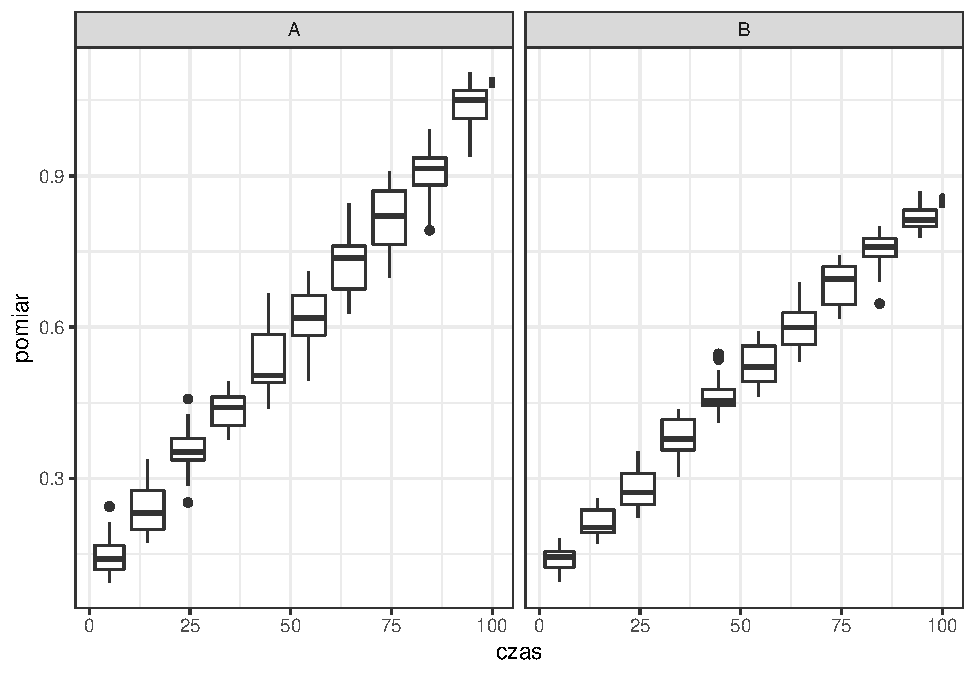
\includegraphics{_main_files/figure-latex/unnamed-chunk-47-1.pdf}

\begin{Shaded}
\begin{Highlighting}[]
\CommentTok{\# Wszystkie słupki tej samej wysokości}
\NormalTok{p }\SpecialCharTok{+} \FunctionTok{geom\_bar}\NormalTok{(}\AttributeTok{position =} \StringTok{"fill"}\NormalTok{) }\SpecialCharTok{+} \FunctionTok{facet\_wrap}\NormalTok{(}\SpecialCharTok{\textasciitilde{}}\NormalTok{ warunki)}
\end{Highlighting}
\end{Shaded}

\begin{verbatim}
## Warning in grid.Call(C_textBounds, as.graphicsAnnot(x$label), x$x, x$y, :
## conversion failure on 'Może' in 'mbcsToSbcs': dot substituted for <c5>
\end{verbatim}

\begin{verbatim}
## Warning in grid.Call(C_textBounds, as.graphicsAnnot(x$label), x$x, x$y, :
## conversion failure on 'Może' in 'mbcsToSbcs': dot substituted for <bc>
\end{verbatim}

\begin{verbatim}
## Warning in grid.Call(C_textBounds, as.graphicsAnnot(x$label), x$x, x$y, :
## conversion failure on 'Może' in 'mbcsToSbcs': dot substituted for <c5>
\end{verbatim}

\begin{verbatim}
## Warning in grid.Call(C_textBounds, as.graphicsAnnot(x$label), x$x, x$y, :
## conversion failure on 'Może' in 'mbcsToSbcs': dot substituted for <bc>
\end{verbatim}

\begin{verbatim}
## Warning in grid.Call(C_textBounds, as.graphicsAnnot(x$label), x$x, x$y, :
## conversion failure on 'Może' in 'mbcsToSbcs': dot substituted for <c5>
\end{verbatim}

\begin{verbatim}
## Warning in grid.Call(C_textBounds, as.graphicsAnnot(x$label), x$x, x$y, :
## conversion failure on 'Może' in 'mbcsToSbcs': dot substituted for <bc>
\end{verbatim}

\begin{verbatim}
## Warning in grid.Call(C_textBounds, as.graphicsAnnot(x$label), x$x, x$y, :
## conversion failure on 'Może' in 'mbcsToSbcs': dot substituted for <c5>
\end{verbatim}

\begin{verbatim}
## Warning in grid.Call(C_textBounds, as.graphicsAnnot(x$label), x$x, x$y, :
## conversion failure on 'Może' in 'mbcsToSbcs': dot substituted for <bc>
\end{verbatim}

\begin{verbatim}
## Warning in grid.Call(C_textBounds, as.graphicsAnnot(x$label), x$x, x$y, :
## conversion failure on 'Może' in 'mbcsToSbcs': dot substituted for <c5>
\end{verbatim}

\begin{verbatim}
## Warning in grid.Call(C_textBounds, as.graphicsAnnot(x$label), x$x, x$y, :
## conversion failure on 'Może' in 'mbcsToSbcs': dot substituted for <bc>
\end{verbatim}

\begin{verbatim}
## Warning in grid.Call(C_textBounds, as.graphicsAnnot(x$label), x$x, x$y, :
## conversion failure on 'Może' in 'mbcsToSbcs': dot substituted for <c5>
\end{verbatim}

\begin{verbatim}
## Warning in grid.Call(C_textBounds, as.graphicsAnnot(x$label), x$x, x$y, :
## conversion failure on 'Może' in 'mbcsToSbcs': dot substituted for <bc>
\end{verbatim}

\begin{verbatim}
## Warning in grid.Call(C_textBounds, as.graphicsAnnot(x$label), x$x, x$y, :
## conversion failure on 'Może' in 'mbcsToSbcs': dot substituted for <c5>
\end{verbatim}

\begin{verbatim}
## Warning in grid.Call(C_textBounds, as.graphicsAnnot(x$label), x$x, x$y, :
## conversion failure on 'Może' in 'mbcsToSbcs': dot substituted for <bc>
\end{verbatim}

\begin{verbatim}
## Warning in grid.Call(C_textBounds, as.graphicsAnnot(x$label), x$x, x$y, :
## conversion failure on 'Może' in 'mbcsToSbcs': dot substituted for <c5>
\end{verbatim}

\begin{verbatim}
## Warning in grid.Call(C_textBounds, as.graphicsAnnot(x$label), x$x, x$y, :
## conversion failure on 'Może' in 'mbcsToSbcs': dot substituted for <bc>
\end{verbatim}

\begin{verbatim}
## Warning in grid.Call(C_textBounds, as.graphicsAnnot(x$label), x$x, x$y, :
## conversion failure on 'Może' in 'mbcsToSbcs': dot substituted for <c5>
\end{verbatim}

\begin{verbatim}
## Warning in grid.Call(C_textBounds, as.graphicsAnnot(x$label), x$x, x$y, :
## conversion failure on 'Może' in 'mbcsToSbcs': dot substituted for <bc>
\end{verbatim}

\begin{verbatim}
## Warning in grid.Call(C_textBounds, as.graphicsAnnot(x$label), x$x, x$y, :
## conversion failure on 'Może' in 'mbcsToSbcs': dot substituted for <c5>
\end{verbatim}

\begin{verbatim}
## Warning in grid.Call(C_textBounds, as.graphicsAnnot(x$label), x$x, x$y, :
## conversion failure on 'Może' in 'mbcsToSbcs': dot substituted for <bc>
\end{verbatim}

\begin{verbatim}
## Warning in grid.Call(C_textBounds, as.graphicsAnnot(x$label), x$x, x$y, :
## conversion failure on 'Może' in 'mbcsToSbcs': dot substituted for <c5>
\end{verbatim}

\begin{verbatim}
## Warning in grid.Call(C_textBounds, as.graphicsAnnot(x$label), x$x, x$y, :
## conversion failure on 'Może' in 'mbcsToSbcs': dot substituted for <bc>
\end{verbatim}

\begin{verbatim}
## Warning in grid.Call(C_textBounds, as.graphicsAnnot(x$label), x$x, x$y, :
## conversion failure on 'Może' in 'mbcsToSbcs': dot substituted for <c5>
\end{verbatim}

\begin{verbatim}
## Warning in grid.Call(C_textBounds, as.graphicsAnnot(x$label), x$x, x$y, :
## conversion failure on 'Może' in 'mbcsToSbcs': dot substituted for <bc>
\end{verbatim}

\begin{verbatim}
## Warning in grid.Call(C_textBounds, as.graphicsAnnot(x$label), x$x, x$y, :
## conversion failure on 'Może' in 'mbcsToSbcs': dot substituted for <c5>
\end{verbatim}

\begin{verbatim}
## Warning in grid.Call(C_textBounds, as.graphicsAnnot(x$label), x$x, x$y, :
## conversion failure on 'Może' in 'mbcsToSbcs': dot substituted for <bc>
\end{verbatim}

\begin{verbatim}
## Warning in grid.Call(C_textBounds, as.graphicsAnnot(x$label), x$x, x$y, :
## conversion failure on 'Może' in 'mbcsToSbcs': dot substituted for <c5>
\end{verbatim}

\begin{verbatim}
## Warning in grid.Call(C_textBounds, as.graphicsAnnot(x$label), x$x, x$y, :
## conversion failure on 'Może' in 'mbcsToSbcs': dot substituted for <bc>
\end{verbatim}

\begin{verbatim}
## Warning in grid.Call(C_textBounds, as.graphicsAnnot(x$label), x$x, x$y, :
## conversion failure on 'Może' in 'mbcsToSbcs': dot substituted for <c5>
\end{verbatim}

\begin{verbatim}
## Warning in grid.Call(C_textBounds, as.graphicsAnnot(x$label), x$x, x$y, :
## conversion failure on 'Może' in 'mbcsToSbcs': dot substituted for <bc>
\end{verbatim}

\begin{verbatim}
## Warning in grid.Call(C_textBounds, as.graphicsAnnot(x$label), x$x, x$y, :
## conversion failure on 'Może' in 'mbcsToSbcs': dot substituted for <c5>
\end{verbatim}

\begin{verbatim}
## Warning in grid.Call(C_textBounds, as.graphicsAnnot(x$label), x$x, x$y, :
## conversion failure on 'Może' in 'mbcsToSbcs': dot substituted for <bc>
\end{verbatim}

\begin{verbatim}
## Warning in grid.Call.graphics(C_text, as.graphicsAnnot(x$label), x$x, x$y, :
## conversion failure on 'Może' in 'mbcsToSbcs': dot substituted for <c5>
\end{verbatim}

\begin{verbatim}
## Warning in grid.Call.graphics(C_text, as.graphicsAnnot(x$label), x$x, x$y, :
## conversion failure on 'Może' in 'mbcsToSbcs': dot substituted for <bc>
\end{verbatim}

\begin{verbatim}
## Warning in grid.Call(C_textBounds, as.graphicsAnnot(x$label), x$x, x$y, :
## conversion failure on 'Może' in 'mbcsToSbcs': dot substituted for <c5>
\end{verbatim}

\begin{verbatim}
## Warning in grid.Call(C_textBounds, as.graphicsAnnot(x$label), x$x, x$y, :
## conversion failure on 'Może' in 'mbcsToSbcs': dot substituted for <bc>
\end{verbatim}

\begin{verbatim}
## Warning in grid.Call(C_textBounds, as.graphicsAnnot(x$label), x$x, x$y, :
## conversion failure on 'Może' in 'mbcsToSbcs': dot substituted for <c5>
\end{verbatim}

\begin{verbatim}
## Warning in grid.Call(C_textBounds, as.graphicsAnnot(x$label), x$x, x$y, :
## conversion failure on 'Może' in 'mbcsToSbcs': dot substituted for <bc>
\end{verbatim}

\begin{verbatim}
## Warning in grid.Call(C_textBounds, as.graphicsAnnot(x$label), x$x, x$y, :
## conversion failure on 'Może' in 'mbcsToSbcs': dot substituted for <c5>
\end{verbatim}

\begin{verbatim}
## Warning in grid.Call(C_textBounds, as.graphicsAnnot(x$label), x$x, x$y, :
## conversion failure on 'Może' in 'mbcsToSbcs': dot substituted for <bc>
\end{verbatim}

\begin{verbatim}
## Warning in grid.Call(C_textBounds, as.graphicsAnnot(x$label), x$x, x$y, :
## conversion failure on 'Może' in 'mbcsToSbcs': dot substituted for <c5>
\end{verbatim}

\begin{verbatim}
## Warning in grid.Call(C_textBounds, as.graphicsAnnot(x$label), x$x, x$y, :
## conversion failure on 'Może' in 'mbcsToSbcs': dot substituted for <bc>
\end{verbatim}

\begin{verbatim}
## Warning in grid.Call(C_textBounds, as.graphicsAnnot(x$label), x$x, x$y, :
## conversion failure on 'Może' in 'mbcsToSbcs': dot substituted for <c5>
\end{verbatim}

\begin{verbatim}
## Warning in grid.Call(C_textBounds, as.graphicsAnnot(x$label), x$x, x$y, :
## conversion failure on 'Może' in 'mbcsToSbcs': dot substituted for <bc>
\end{verbatim}

\begin{verbatim}
## Warning in grid.Call(C_textBounds, as.graphicsAnnot(x$label), x$x, x$y, :
## conversion failure on 'Może' in 'mbcsToSbcs': dot substituted for <c5>
\end{verbatim}

\begin{verbatim}
## Warning in grid.Call(C_textBounds, as.graphicsAnnot(x$label), x$x, x$y, :
## conversion failure on 'Może' in 'mbcsToSbcs': dot substituted for <bc>
\end{verbatim}

\begin{verbatim}
## Warning in grid.Call(C_textBounds, as.graphicsAnnot(x$label), x$x, x$y, :
## conversion failure on 'Może' in 'mbcsToSbcs': dot substituted for <c5>
\end{verbatim}

\begin{verbatim}
## Warning in grid.Call(C_textBounds, as.graphicsAnnot(x$label), x$x, x$y, :
## conversion failure on 'Może' in 'mbcsToSbcs': dot substituted for <bc>
\end{verbatim}

\begin{verbatim}
## Warning in grid.Call(C_textBounds, as.graphicsAnnot(x$label), x$x, x$y, :
## conversion failure on 'Może' in 'mbcsToSbcs': dot substituted for <c5>
\end{verbatim}

\begin{verbatim}
## Warning in grid.Call(C_textBounds, as.graphicsAnnot(x$label), x$x, x$y, :
## conversion failure on 'Może' in 'mbcsToSbcs': dot substituted for <bc>
\end{verbatim}

\begin{verbatim}
## Warning in grid.Call(C_textBounds, as.graphicsAnnot(x$label), x$x, x$y, :
## conversion failure on 'Może' in 'mbcsToSbcs': dot substituted for <c5>
\end{verbatim}

\begin{verbatim}
## Warning in grid.Call(C_textBounds, as.graphicsAnnot(x$label), x$x, x$y, :
## conversion failure on 'Może' in 'mbcsToSbcs': dot substituted for <bc>
\end{verbatim}

\begin{verbatim}
## Warning in grid.Call(C_textBounds, as.graphicsAnnot(x$label), x$x, x$y, :
## conversion failure on 'Może' in 'mbcsToSbcs': dot substituted for <c5>
\end{verbatim}

\begin{verbatim}
## Warning in grid.Call(C_textBounds, as.graphicsAnnot(x$label), x$x, x$y, :
## conversion failure on 'Może' in 'mbcsToSbcs': dot substituted for <bc>
\end{verbatim}

\begin{verbatim}
## Warning in grid.Call.graphics(C_text, as.graphicsAnnot(x$label), x$x, x$y, :
## conversion failure on 'Może' in 'mbcsToSbcs': dot substituted for <c5>
\end{verbatim}

\begin{verbatim}
## Warning in grid.Call.graphics(C_text, as.graphicsAnnot(x$label), x$x, x$y, :
## conversion failure on 'Może' in 'mbcsToSbcs': dot substituted for <bc>
\end{verbatim}

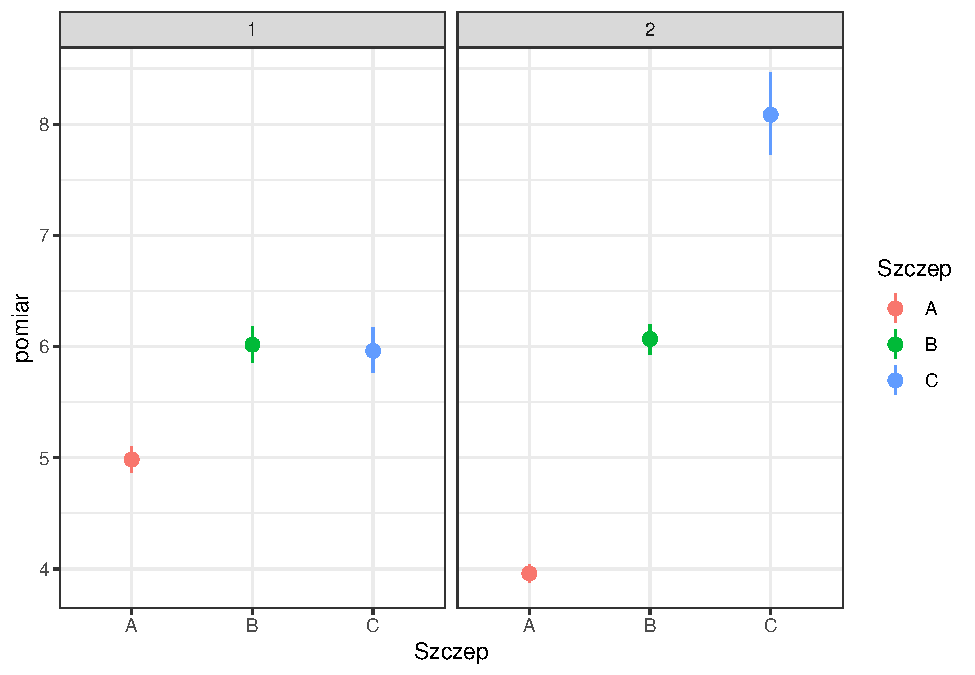
\includegraphics{_main_files/figure-latex/unnamed-chunk-47-2.pdf}

\begin{Shaded}
\begin{Highlighting}[]
\CommentTok{\# Szerokość słupków można zmieniać parametrem width}
\NormalTok{p }\SpecialCharTok{+} \FunctionTok{geom\_bar}\NormalTok{(}\AttributeTok{position =} \StringTok{"dodge"}\NormalTok{, }\AttributeTok{width =} \FloatTok{0.4}\NormalTok{) }\SpecialCharTok{+} \FunctionTok{facet\_wrap}\NormalTok{(}\SpecialCharTok{\textasciitilde{}}\NormalTok{ warunki)}
\end{Highlighting}
\end{Shaded}

\begin{verbatim}
## Warning in grid.Call(C_textBounds, as.graphicsAnnot(x$label), x$x, x$y, :
## conversion failure on 'Może' in 'mbcsToSbcs': dot substituted for <c5>
\end{verbatim}

\begin{verbatim}
## Warning in grid.Call(C_textBounds, as.graphicsAnnot(x$label), x$x, x$y, :
## conversion failure on 'Może' in 'mbcsToSbcs': dot substituted for <bc>
\end{verbatim}

\begin{verbatim}
## Warning in grid.Call(C_textBounds, as.graphicsAnnot(x$label), x$x, x$y, :
## conversion failure on 'Może' in 'mbcsToSbcs': dot substituted for <c5>
\end{verbatim}

\begin{verbatim}
## Warning in grid.Call(C_textBounds, as.graphicsAnnot(x$label), x$x, x$y, :
## conversion failure on 'Może' in 'mbcsToSbcs': dot substituted for <bc>
\end{verbatim}

\begin{verbatim}
## Warning in grid.Call(C_textBounds, as.graphicsAnnot(x$label), x$x, x$y, :
## conversion failure on 'Może' in 'mbcsToSbcs': dot substituted for <c5>
\end{verbatim}

\begin{verbatim}
## Warning in grid.Call(C_textBounds, as.graphicsAnnot(x$label), x$x, x$y, :
## conversion failure on 'Może' in 'mbcsToSbcs': dot substituted for <bc>
\end{verbatim}

\begin{verbatim}
## Warning in grid.Call(C_textBounds, as.graphicsAnnot(x$label), x$x, x$y, :
## conversion failure on 'Może' in 'mbcsToSbcs': dot substituted for <c5>
\end{verbatim}

\begin{verbatim}
## Warning in grid.Call(C_textBounds, as.graphicsAnnot(x$label), x$x, x$y, :
## conversion failure on 'Może' in 'mbcsToSbcs': dot substituted for <bc>
\end{verbatim}

\begin{verbatim}
## Warning in grid.Call(C_textBounds, as.graphicsAnnot(x$label), x$x, x$y, :
## conversion failure on 'Może' in 'mbcsToSbcs': dot substituted for <c5>
\end{verbatim}

\begin{verbatim}
## Warning in grid.Call(C_textBounds, as.graphicsAnnot(x$label), x$x, x$y, :
## conversion failure on 'Może' in 'mbcsToSbcs': dot substituted for <bc>
\end{verbatim}

\begin{verbatim}
## Warning in grid.Call(C_textBounds, as.graphicsAnnot(x$label), x$x, x$y, :
## conversion failure on 'Może' in 'mbcsToSbcs': dot substituted for <c5>
\end{verbatim}

\begin{verbatim}
## Warning in grid.Call(C_textBounds, as.graphicsAnnot(x$label), x$x, x$y, :
## conversion failure on 'Może' in 'mbcsToSbcs': dot substituted for <bc>
\end{verbatim}

\begin{verbatim}
## Warning in grid.Call(C_textBounds, as.graphicsAnnot(x$label), x$x, x$y, :
## conversion failure on 'Może' in 'mbcsToSbcs': dot substituted for <c5>
\end{verbatim}

\begin{verbatim}
## Warning in grid.Call(C_textBounds, as.graphicsAnnot(x$label), x$x, x$y, :
## conversion failure on 'Może' in 'mbcsToSbcs': dot substituted for <bc>
\end{verbatim}

\begin{verbatim}
## Warning in grid.Call(C_textBounds, as.graphicsAnnot(x$label), x$x, x$y, :
## conversion failure on 'Może' in 'mbcsToSbcs': dot substituted for <c5>
\end{verbatim}

\begin{verbatim}
## Warning in grid.Call(C_textBounds, as.graphicsAnnot(x$label), x$x, x$y, :
## conversion failure on 'Może' in 'mbcsToSbcs': dot substituted for <bc>
\end{verbatim}

\begin{verbatim}
## Warning in grid.Call(C_textBounds, as.graphicsAnnot(x$label), x$x, x$y, :
## conversion failure on 'Może' in 'mbcsToSbcs': dot substituted for <c5>
\end{verbatim}

\begin{verbatim}
## Warning in grid.Call(C_textBounds, as.graphicsAnnot(x$label), x$x, x$y, :
## conversion failure on 'Może' in 'mbcsToSbcs': dot substituted for <bc>
\end{verbatim}

\begin{verbatim}
## Warning in grid.Call(C_textBounds, as.graphicsAnnot(x$label), x$x, x$y, :
## conversion failure on 'Może' in 'mbcsToSbcs': dot substituted for <c5>
\end{verbatim}

\begin{verbatim}
## Warning in grid.Call(C_textBounds, as.graphicsAnnot(x$label), x$x, x$y, :
## conversion failure on 'Może' in 'mbcsToSbcs': dot substituted for <bc>
\end{verbatim}

\begin{verbatim}
## Warning in grid.Call(C_textBounds, as.graphicsAnnot(x$label), x$x, x$y, :
## conversion failure on 'Może' in 'mbcsToSbcs': dot substituted for <c5>
\end{verbatim}

\begin{verbatim}
## Warning in grid.Call(C_textBounds, as.graphicsAnnot(x$label), x$x, x$y, :
## conversion failure on 'Może' in 'mbcsToSbcs': dot substituted for <bc>
\end{verbatim}

\begin{verbatim}
## Warning in grid.Call(C_textBounds, as.graphicsAnnot(x$label), x$x, x$y, :
## conversion failure on 'Może' in 'mbcsToSbcs': dot substituted for <c5>
\end{verbatim}

\begin{verbatim}
## Warning in grid.Call(C_textBounds, as.graphicsAnnot(x$label), x$x, x$y, :
## conversion failure on 'Może' in 'mbcsToSbcs': dot substituted for <bc>
\end{verbatim}

\begin{verbatim}
## Warning in grid.Call(C_textBounds, as.graphicsAnnot(x$label), x$x, x$y, :
## conversion failure on 'Może' in 'mbcsToSbcs': dot substituted for <c5>
\end{verbatim}

\begin{verbatim}
## Warning in grid.Call(C_textBounds, as.graphicsAnnot(x$label), x$x, x$y, :
## conversion failure on 'Może' in 'mbcsToSbcs': dot substituted for <bc>
\end{verbatim}

\begin{verbatim}
## Warning in grid.Call(C_textBounds, as.graphicsAnnot(x$label), x$x, x$y, :
## conversion failure on 'Może' in 'mbcsToSbcs': dot substituted for <c5>
\end{verbatim}

\begin{verbatim}
## Warning in grid.Call(C_textBounds, as.graphicsAnnot(x$label), x$x, x$y, :
## conversion failure on 'Może' in 'mbcsToSbcs': dot substituted for <bc>
\end{verbatim}

\begin{verbatim}
## Warning in grid.Call(C_textBounds, as.graphicsAnnot(x$label), x$x, x$y, :
## conversion failure on 'Może' in 'mbcsToSbcs': dot substituted for <c5>
\end{verbatim}

\begin{verbatim}
## Warning in grid.Call(C_textBounds, as.graphicsAnnot(x$label), x$x, x$y, :
## conversion failure on 'Może' in 'mbcsToSbcs': dot substituted for <bc>
\end{verbatim}

\begin{verbatim}
## Warning in grid.Call(C_textBounds, as.graphicsAnnot(x$label), x$x, x$y, :
## conversion failure on 'Może' in 'mbcsToSbcs': dot substituted for <c5>
\end{verbatim}

\begin{verbatim}
## Warning in grid.Call(C_textBounds, as.graphicsAnnot(x$label), x$x, x$y, :
## conversion failure on 'Może' in 'mbcsToSbcs': dot substituted for <bc>
\end{verbatim}

\begin{verbatim}
## Warning in grid.Call.graphics(C_text, as.graphicsAnnot(x$label), x$x, x$y, :
## conversion failure on 'Może' in 'mbcsToSbcs': dot substituted for <c5>
\end{verbatim}

\begin{verbatim}
## Warning in grid.Call.graphics(C_text, as.graphicsAnnot(x$label), x$x, x$y, :
## conversion failure on 'Może' in 'mbcsToSbcs': dot substituted for <bc>
\end{verbatim}

\begin{verbatim}
## Warning in grid.Call(C_textBounds, as.graphicsAnnot(x$label), x$x, x$y, :
## conversion failure on 'Może' in 'mbcsToSbcs': dot substituted for <c5>
\end{verbatim}

\begin{verbatim}
## Warning in grid.Call(C_textBounds, as.graphicsAnnot(x$label), x$x, x$y, :
## conversion failure on 'Może' in 'mbcsToSbcs': dot substituted for <bc>
\end{verbatim}

\begin{verbatim}
## Warning in grid.Call(C_textBounds, as.graphicsAnnot(x$label), x$x, x$y, :
## conversion failure on 'Może' in 'mbcsToSbcs': dot substituted for <c5>
\end{verbatim}

\begin{verbatim}
## Warning in grid.Call(C_textBounds, as.graphicsAnnot(x$label), x$x, x$y, :
## conversion failure on 'Może' in 'mbcsToSbcs': dot substituted for <bc>
\end{verbatim}

\begin{verbatim}
## Warning in grid.Call(C_textBounds, as.graphicsAnnot(x$label), x$x, x$y, :
## conversion failure on 'Może' in 'mbcsToSbcs': dot substituted for <c5>
\end{verbatim}

\begin{verbatim}
## Warning in grid.Call(C_textBounds, as.graphicsAnnot(x$label), x$x, x$y, :
## conversion failure on 'Może' in 'mbcsToSbcs': dot substituted for <bc>
\end{verbatim}

\begin{verbatim}
## Warning in grid.Call(C_textBounds, as.graphicsAnnot(x$label), x$x, x$y, :
## conversion failure on 'Może' in 'mbcsToSbcs': dot substituted for <c5>
\end{verbatim}

\begin{verbatim}
## Warning in grid.Call(C_textBounds, as.graphicsAnnot(x$label), x$x, x$y, :
## conversion failure on 'Może' in 'mbcsToSbcs': dot substituted for <bc>
\end{verbatim}

\begin{verbatim}
## Warning in grid.Call(C_textBounds, as.graphicsAnnot(x$label), x$x, x$y, :
## conversion failure on 'Może' in 'mbcsToSbcs': dot substituted for <c5>
\end{verbatim}

\begin{verbatim}
## Warning in grid.Call(C_textBounds, as.graphicsAnnot(x$label), x$x, x$y, :
## conversion failure on 'Może' in 'mbcsToSbcs': dot substituted for <bc>
\end{verbatim}

\begin{verbatim}
## Warning in grid.Call(C_textBounds, as.graphicsAnnot(x$label), x$x, x$y, :
## conversion failure on 'Może' in 'mbcsToSbcs': dot substituted for <c5>
\end{verbatim}

\begin{verbatim}
## Warning in grid.Call(C_textBounds, as.graphicsAnnot(x$label), x$x, x$y, :
## conversion failure on 'Może' in 'mbcsToSbcs': dot substituted for <bc>
\end{verbatim}

\begin{verbatim}
## Warning in grid.Call(C_textBounds, as.graphicsAnnot(x$label), x$x, x$y, :
## conversion failure on 'Może' in 'mbcsToSbcs': dot substituted for <c5>
\end{verbatim}

\begin{verbatim}
## Warning in grid.Call(C_textBounds, as.graphicsAnnot(x$label), x$x, x$y, :
## conversion failure on 'Może' in 'mbcsToSbcs': dot substituted for <bc>
\end{verbatim}

\begin{verbatim}
## Warning in grid.Call(C_textBounds, as.graphicsAnnot(x$label), x$x, x$y, :
## conversion failure on 'Może' in 'mbcsToSbcs': dot substituted for <c5>
\end{verbatim}

\begin{verbatim}
## Warning in grid.Call(C_textBounds, as.graphicsAnnot(x$label), x$x, x$y, :
## conversion failure on 'Może' in 'mbcsToSbcs': dot substituted for <bc>
\end{verbatim}

\begin{verbatim}
## Warning in grid.Call(C_textBounds, as.graphicsAnnot(x$label), x$x, x$y, :
## conversion failure on 'Może' in 'mbcsToSbcs': dot substituted for <c5>
\end{verbatim}

\begin{verbatim}
## Warning in grid.Call(C_textBounds, as.graphicsAnnot(x$label), x$x, x$y, :
## conversion failure on 'Może' in 'mbcsToSbcs': dot substituted for <bc>
\end{verbatim}

\begin{verbatim}
## Warning in grid.Call(C_textBounds, as.graphicsAnnot(x$label), x$x, x$y, :
## conversion failure on 'Może' in 'mbcsToSbcs': dot substituted for <c5>
\end{verbatim}

\begin{verbatim}
## Warning in grid.Call(C_textBounds, as.graphicsAnnot(x$label), x$x, x$y, :
## conversion failure on 'Może' in 'mbcsToSbcs': dot substituted for <bc>
\end{verbatim}

\begin{verbatim}
## Warning in grid.Call.graphics(C_text, as.graphicsAnnot(x$label), x$x, x$y, :
## conversion failure on 'Może' in 'mbcsToSbcs': dot substituted for <c5>
\end{verbatim}

\begin{verbatim}
## Warning in grid.Call.graphics(C_text, as.graphicsAnnot(x$label), x$x, x$y, :
## conversion failure on 'Może' in 'mbcsToSbcs': dot substituted for <bc>
\end{verbatim}

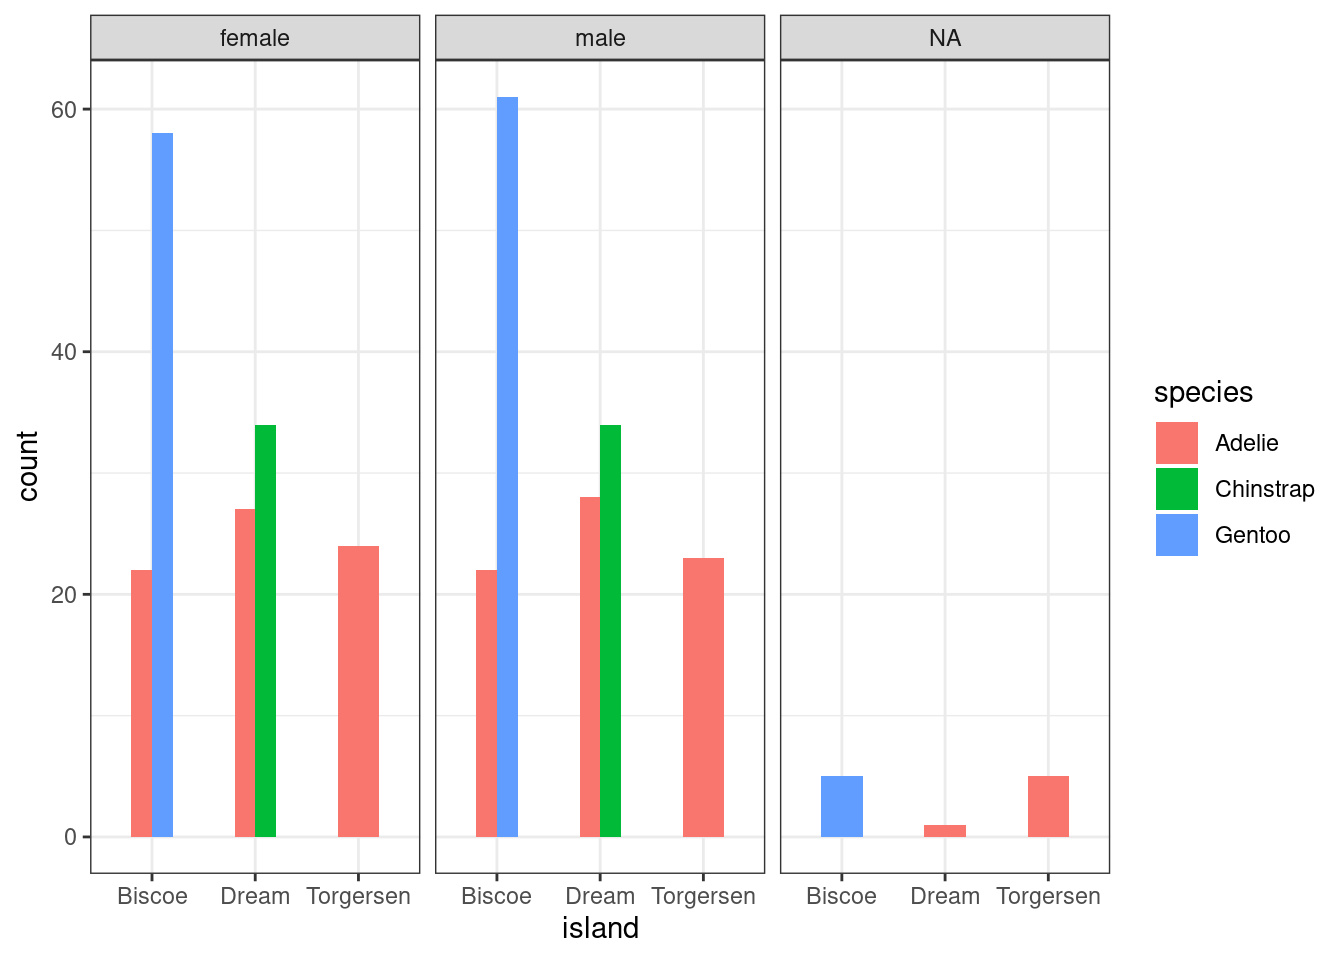
\includegraphics{_main_files/figure-latex/unnamed-chunk-47-3.pdf}

\begin{Shaded}
\begin{Highlighting}[]
\CommentTok{\# Wykres bez wartości NA, filter można zrobić też wcześniej albo w obrębie ggplot}
\NormalTok{p }\OtherTok{\textless{}{-}} \FunctionTok{ggplot}\NormalTok{(dane2 }\SpecialCharTok{\%\textgreater{}\%} \FunctionTok{filter}\NormalTok{(}\SpecialCharTok{!}\FunctionTok{is.na}\NormalTok{(pomiar)), }\FunctionTok{aes}\NormalTok{(}\AttributeTok{x =}\NormalTok{ pomiar, }\AttributeTok{fill =}\NormalTok{ Szczep))}
\NormalTok{p }\SpecialCharTok{+} \FunctionTok{geom\_bar}\NormalTok{(}\AttributeTok{position =} \StringTok{"dodge"}\NormalTok{) }\SpecialCharTok{+} \FunctionTok{facet\_wrap}\NormalTok{(}\SpecialCharTok{\textasciitilde{}}\NormalTok{ warunki)}
\end{Highlighting}
\end{Shaded}

\begin{verbatim}
## Warning in grid.Call(C_textBounds, as.graphicsAnnot(x$label), x$x, x$y, :
## conversion failure on 'Może' in 'mbcsToSbcs': dot substituted for <c5>
\end{verbatim}

\begin{verbatim}
## Warning in grid.Call(C_textBounds, as.graphicsAnnot(x$label), x$x, x$y, :
## conversion failure on 'Może' in 'mbcsToSbcs': dot substituted for <bc>
\end{verbatim}

\begin{verbatim}
## Warning in grid.Call(C_textBounds, as.graphicsAnnot(x$label), x$x, x$y, :
## conversion failure on 'Może' in 'mbcsToSbcs': dot substituted for <c5>
\end{verbatim}

\begin{verbatim}
## Warning in grid.Call(C_textBounds, as.graphicsAnnot(x$label), x$x, x$y, :
## conversion failure on 'Może' in 'mbcsToSbcs': dot substituted for <bc>
\end{verbatim}

\begin{verbatim}
## Warning in grid.Call(C_textBounds, as.graphicsAnnot(x$label), x$x, x$y, :
## conversion failure on 'Może' in 'mbcsToSbcs': dot substituted for <c5>
\end{verbatim}

\begin{verbatim}
## Warning in grid.Call(C_textBounds, as.graphicsAnnot(x$label), x$x, x$y, :
## conversion failure on 'Może' in 'mbcsToSbcs': dot substituted for <bc>
\end{verbatim}

\begin{verbatim}
## Warning in grid.Call(C_textBounds, as.graphicsAnnot(x$label), x$x, x$y, :
## conversion failure on 'Może' in 'mbcsToSbcs': dot substituted for <c5>
\end{verbatim}

\begin{verbatim}
## Warning in grid.Call(C_textBounds, as.graphicsAnnot(x$label), x$x, x$y, :
## conversion failure on 'Może' in 'mbcsToSbcs': dot substituted for <bc>
\end{verbatim}

\begin{verbatim}
## Warning in grid.Call(C_textBounds, as.graphicsAnnot(x$label), x$x, x$y, :
## conversion failure on 'Może' in 'mbcsToSbcs': dot substituted for <c5>
\end{verbatim}

\begin{verbatim}
## Warning in grid.Call(C_textBounds, as.graphicsAnnot(x$label), x$x, x$y, :
## conversion failure on 'Może' in 'mbcsToSbcs': dot substituted for <bc>
\end{verbatim}

\begin{verbatim}
## Warning in grid.Call(C_textBounds, as.graphicsAnnot(x$label), x$x, x$y, :
## conversion failure on 'Może' in 'mbcsToSbcs': dot substituted for <c5>
\end{verbatim}

\begin{verbatim}
## Warning in grid.Call(C_textBounds, as.graphicsAnnot(x$label), x$x, x$y, :
## conversion failure on 'Może' in 'mbcsToSbcs': dot substituted for <bc>
\end{verbatim}

\begin{verbatim}
## Warning in grid.Call(C_textBounds, as.graphicsAnnot(x$label), x$x, x$y, :
## conversion failure on 'Może' in 'mbcsToSbcs': dot substituted for <c5>
\end{verbatim}

\begin{verbatim}
## Warning in grid.Call(C_textBounds, as.graphicsAnnot(x$label), x$x, x$y, :
## conversion failure on 'Może' in 'mbcsToSbcs': dot substituted for <bc>
\end{verbatim}

\begin{verbatim}
## Warning in grid.Call(C_textBounds, as.graphicsAnnot(x$label), x$x, x$y, :
## conversion failure on 'Może' in 'mbcsToSbcs': dot substituted for <c5>
\end{verbatim}

\begin{verbatim}
## Warning in grid.Call(C_textBounds, as.graphicsAnnot(x$label), x$x, x$y, :
## conversion failure on 'Może' in 'mbcsToSbcs': dot substituted for <bc>
\end{verbatim}

\begin{verbatim}
## Warning in grid.Call(C_textBounds, as.graphicsAnnot(x$label), x$x, x$y, :
## conversion failure on 'Może' in 'mbcsToSbcs': dot substituted for <c5>
\end{verbatim}

\begin{verbatim}
## Warning in grid.Call(C_textBounds, as.graphicsAnnot(x$label), x$x, x$y, :
## conversion failure on 'Może' in 'mbcsToSbcs': dot substituted for <bc>
\end{verbatim}

\begin{verbatim}
## Warning in grid.Call(C_textBounds, as.graphicsAnnot(x$label), x$x, x$y, :
## conversion failure on 'Może' in 'mbcsToSbcs': dot substituted for <c5>
\end{verbatim}

\begin{verbatim}
## Warning in grid.Call(C_textBounds, as.graphicsAnnot(x$label), x$x, x$y, :
## conversion failure on 'Może' in 'mbcsToSbcs': dot substituted for <bc>
\end{verbatim}

\begin{verbatim}
## Warning in grid.Call(C_textBounds, as.graphicsAnnot(x$label), x$x, x$y, :
## conversion failure on 'Może' in 'mbcsToSbcs': dot substituted for <c5>
\end{verbatim}

\begin{verbatim}
## Warning in grid.Call(C_textBounds, as.graphicsAnnot(x$label), x$x, x$y, :
## conversion failure on 'Może' in 'mbcsToSbcs': dot substituted for <bc>
\end{verbatim}

\begin{verbatim}
## Warning in grid.Call(C_textBounds, as.graphicsAnnot(x$label), x$x, x$y, :
## conversion failure on 'Może' in 'mbcsToSbcs': dot substituted for <c5>
\end{verbatim}

\begin{verbatim}
## Warning in grid.Call(C_textBounds, as.graphicsAnnot(x$label), x$x, x$y, :
## conversion failure on 'Może' in 'mbcsToSbcs': dot substituted for <bc>
\end{verbatim}

\begin{verbatim}
## Warning in grid.Call(C_textBounds, as.graphicsAnnot(x$label), x$x, x$y, :
## conversion failure on 'Może' in 'mbcsToSbcs': dot substituted for <c5>
\end{verbatim}

\begin{verbatim}
## Warning in grid.Call(C_textBounds, as.graphicsAnnot(x$label), x$x, x$y, :
## conversion failure on 'Może' in 'mbcsToSbcs': dot substituted for <bc>
\end{verbatim}

\begin{verbatim}
## Warning in grid.Call(C_textBounds, as.graphicsAnnot(x$label), x$x, x$y, :
## conversion failure on 'Może' in 'mbcsToSbcs': dot substituted for <c5>
\end{verbatim}

\begin{verbatim}
## Warning in grid.Call(C_textBounds, as.graphicsAnnot(x$label), x$x, x$y, :
## conversion failure on 'Może' in 'mbcsToSbcs': dot substituted for <bc>
\end{verbatim}

\begin{verbatim}
## Warning in grid.Call(C_textBounds, as.graphicsAnnot(x$label), x$x, x$y, :
## conversion failure on 'Może' in 'mbcsToSbcs': dot substituted for <c5>
\end{verbatim}

\begin{verbatim}
## Warning in grid.Call(C_textBounds, as.graphicsAnnot(x$label), x$x, x$y, :
## conversion failure on 'Może' in 'mbcsToSbcs': dot substituted for <bc>
\end{verbatim}

\begin{verbatim}
## Warning in grid.Call(C_textBounds, as.graphicsAnnot(x$label), x$x, x$y, :
## conversion failure on 'Może' in 'mbcsToSbcs': dot substituted for <c5>
\end{verbatim}

\begin{verbatim}
## Warning in grid.Call(C_textBounds, as.graphicsAnnot(x$label), x$x, x$y, :
## conversion failure on 'Może' in 'mbcsToSbcs': dot substituted for <bc>
\end{verbatim}

\begin{verbatim}
## Warning in grid.Call.graphics(C_text, as.graphicsAnnot(x$label), x$x, x$y, :
## conversion failure on 'Może' in 'mbcsToSbcs': dot substituted for <c5>
\end{verbatim}

\begin{verbatim}
## Warning in grid.Call.graphics(C_text, as.graphicsAnnot(x$label), x$x, x$y, :
## conversion failure on 'Może' in 'mbcsToSbcs': dot substituted for <bc>
\end{verbatim}

\begin{verbatim}
## Warning in grid.Call(C_textBounds, as.graphicsAnnot(x$label), x$x, x$y, :
## conversion failure on 'Może' in 'mbcsToSbcs': dot substituted for <c5>
\end{verbatim}

\begin{verbatim}
## Warning in grid.Call(C_textBounds, as.graphicsAnnot(x$label), x$x, x$y, :
## conversion failure on 'Może' in 'mbcsToSbcs': dot substituted for <bc>
\end{verbatim}

\begin{verbatim}
## Warning in grid.Call(C_textBounds, as.graphicsAnnot(x$label), x$x, x$y, :
## conversion failure on 'Może' in 'mbcsToSbcs': dot substituted for <c5>
\end{verbatim}

\begin{verbatim}
## Warning in grid.Call(C_textBounds, as.graphicsAnnot(x$label), x$x, x$y, :
## conversion failure on 'Może' in 'mbcsToSbcs': dot substituted for <bc>
\end{verbatim}

\begin{verbatim}
## Warning in grid.Call(C_textBounds, as.graphicsAnnot(x$label), x$x, x$y, :
## conversion failure on 'Może' in 'mbcsToSbcs': dot substituted for <c5>
\end{verbatim}

\begin{verbatim}
## Warning in grid.Call(C_textBounds, as.graphicsAnnot(x$label), x$x, x$y, :
## conversion failure on 'Może' in 'mbcsToSbcs': dot substituted for <bc>
\end{verbatim}

\begin{verbatim}
## Warning in grid.Call(C_textBounds, as.graphicsAnnot(x$label), x$x, x$y, :
## conversion failure on 'Może' in 'mbcsToSbcs': dot substituted for <c5>
\end{verbatim}

\begin{verbatim}
## Warning in grid.Call(C_textBounds, as.graphicsAnnot(x$label), x$x, x$y, :
## conversion failure on 'Może' in 'mbcsToSbcs': dot substituted for <bc>
\end{verbatim}

\begin{verbatim}
## Warning in grid.Call(C_textBounds, as.graphicsAnnot(x$label), x$x, x$y, :
## conversion failure on 'Może' in 'mbcsToSbcs': dot substituted for <c5>
\end{verbatim}

\begin{verbatim}
## Warning in grid.Call(C_textBounds, as.graphicsAnnot(x$label), x$x, x$y, :
## conversion failure on 'Może' in 'mbcsToSbcs': dot substituted for <bc>
\end{verbatim}

\begin{verbatim}
## Warning in grid.Call(C_textBounds, as.graphicsAnnot(x$label), x$x, x$y, :
## conversion failure on 'Może' in 'mbcsToSbcs': dot substituted for <c5>
\end{verbatim}

\begin{verbatim}
## Warning in grid.Call(C_textBounds, as.graphicsAnnot(x$label), x$x, x$y, :
## conversion failure on 'Może' in 'mbcsToSbcs': dot substituted for <bc>
\end{verbatim}

\begin{verbatim}
## Warning in grid.Call(C_textBounds, as.graphicsAnnot(x$label), x$x, x$y, :
## conversion failure on 'Może' in 'mbcsToSbcs': dot substituted for <c5>
\end{verbatim}

\begin{verbatim}
## Warning in grid.Call(C_textBounds, as.graphicsAnnot(x$label), x$x, x$y, :
## conversion failure on 'Może' in 'mbcsToSbcs': dot substituted for <bc>
\end{verbatim}

\begin{verbatim}
## Warning in grid.Call(C_textBounds, as.graphicsAnnot(x$label), x$x, x$y, :
## conversion failure on 'Może' in 'mbcsToSbcs': dot substituted for <c5>
\end{verbatim}

\begin{verbatim}
## Warning in grid.Call(C_textBounds, as.graphicsAnnot(x$label), x$x, x$y, :
## conversion failure on 'Może' in 'mbcsToSbcs': dot substituted for <bc>
\end{verbatim}

\begin{verbatim}
## Warning in grid.Call(C_textBounds, as.graphicsAnnot(x$label), x$x, x$y, :
## conversion failure on 'Może' in 'mbcsToSbcs': dot substituted for <c5>
\end{verbatim}

\begin{verbatim}
## Warning in grid.Call(C_textBounds, as.graphicsAnnot(x$label), x$x, x$y, :
## conversion failure on 'Może' in 'mbcsToSbcs': dot substituted for <bc>
\end{verbatim}

\begin{verbatim}
## Warning in grid.Call(C_textBounds, as.graphicsAnnot(x$label), x$x, x$y, :
## conversion failure on 'Może' in 'mbcsToSbcs': dot substituted for <c5>
\end{verbatim}

\begin{verbatim}
## Warning in grid.Call(C_textBounds, as.graphicsAnnot(x$label), x$x, x$y, :
## conversion failure on 'Może' in 'mbcsToSbcs': dot substituted for <bc>
\end{verbatim}

\begin{verbatim}
## Warning in grid.Call.graphics(C_text, as.graphicsAnnot(x$label), x$x, x$y, :
## conversion failure on 'Może' in 'mbcsToSbcs': dot substituted for <c5>
\end{verbatim}

\begin{verbatim}
## Warning in grid.Call.graphics(C_text, as.graphicsAnnot(x$label), x$x, x$y, :
## conversion failure on 'Może' in 'mbcsToSbcs': dot substituted for <bc>
\end{verbatim}

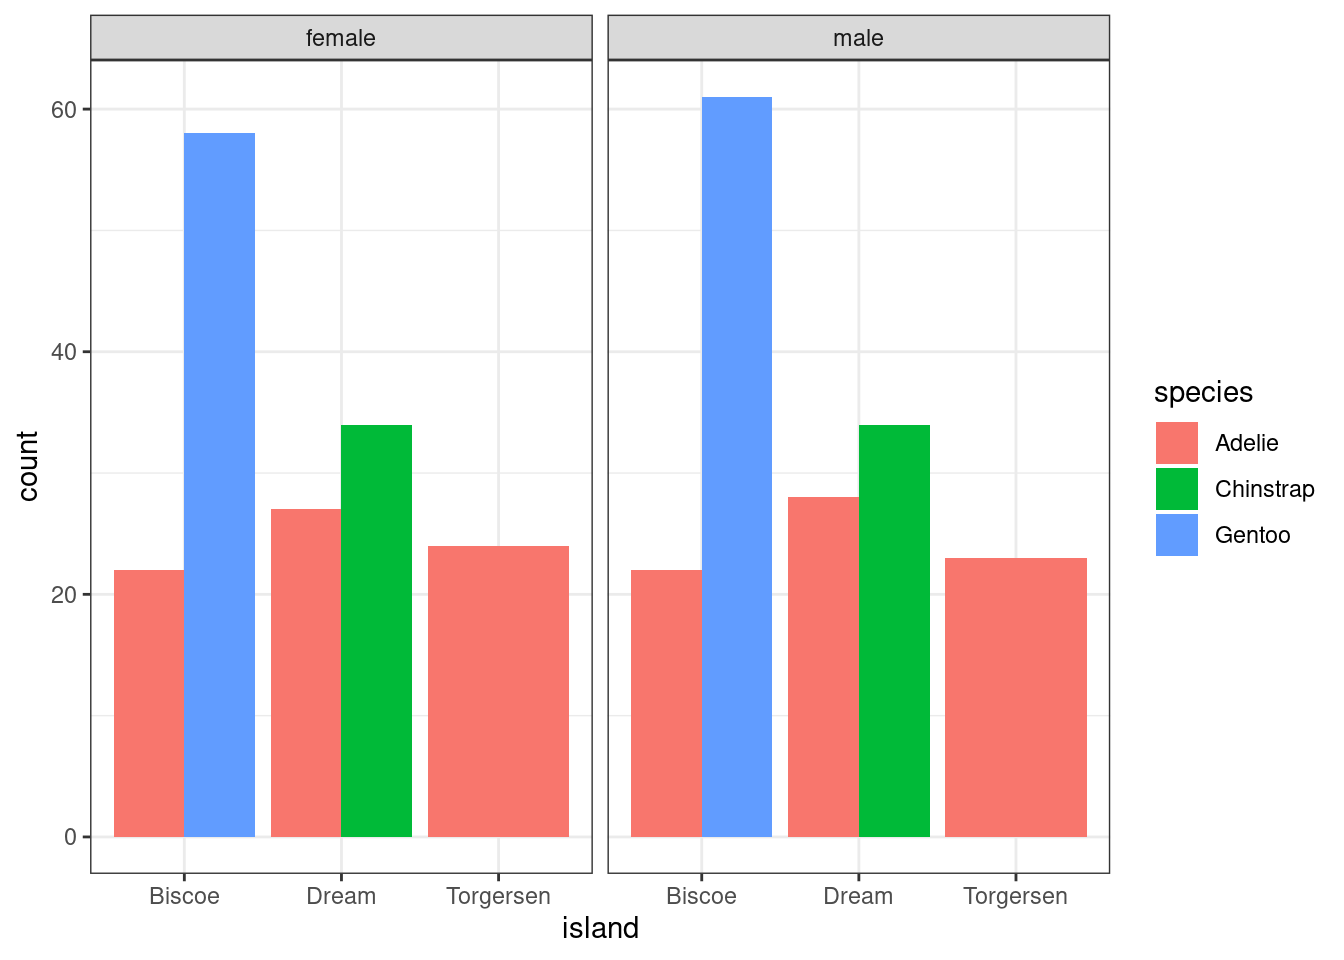
\includegraphics{_main_files/figure-latex/unnamed-chunk-47-4.pdf}

Przy dużej ilości różnokolorowych słupków wykres może być trudny do odczytania. Można wtedy rozważyć zastosowanie dotchart - czyli wykresu na którym wartości zliczenia są oznaczane przez pojedyncze punkty, a nie przez wysokość słupków. W ggplot2 do zrobienia dotchart możemy użyć \texttt{geom\_point}

\begin{Shaded}
\begin{Highlighting}[]
\CommentTok{\# Ustawiamy stat="bin" {-} oznacza że ggplot ma zliczyć częstości występowania elementów,}
\CommentTok{\# a nie narysować każdy z osobna i obracamy wykres {-} ułatwia odczytanie}
\NormalTok{p }\SpecialCharTok{+} \FunctionTok{geom\_point}\NormalTok{(}\AttributeTok{size=}\DecValTok{3}\NormalTok{, }\AttributeTok{stat=}\StringTok{\textquotesingle{}count\textquotesingle{}}\NormalTok{, }\FunctionTok{aes}\NormalTok{(}\AttributeTok{color=}\NormalTok{Szczep))}\SpecialCharTok{+}
  \FunctionTok{facet\_wrap}\NormalTok{(}\SpecialCharTok{\textasciitilde{}}\NormalTok{warunki)}\SpecialCharTok{+}\FunctionTok{coord\_flip}\NormalTok{()}
\end{Highlighting}
\end{Shaded}

\begin{verbatim}
## Warning in grid.Call(C_textBounds, as.graphicsAnnot(x$label), x$x, x$y, :
## conversion failure on 'Może' in 'mbcsToSbcs': dot substituted for <c5>
\end{verbatim}

\begin{verbatim}
## Warning in grid.Call(C_textBounds, as.graphicsAnnot(x$label), x$x, x$y, :
## conversion failure on 'Może' in 'mbcsToSbcs': dot substituted for <bc>
\end{verbatim}

\begin{verbatim}
## Warning in grid.Call(C_textBounds, as.graphicsAnnot(x$label), x$x, x$y, :
## conversion failure on 'Może' in 'mbcsToSbcs': dot substituted for <c5>
\end{verbatim}

\begin{verbatim}
## Warning in grid.Call(C_textBounds, as.graphicsAnnot(x$label), x$x, x$y, :
## conversion failure on 'Może' in 'mbcsToSbcs': dot substituted for <bc>
\end{verbatim}

\begin{verbatim}
## Warning in grid.Call(C_textBounds, as.graphicsAnnot(x$label), x$x, x$y, :
## conversion failure on 'Może' in 'mbcsToSbcs': dot substituted for <c5>
\end{verbatim}

\begin{verbatim}
## Warning in grid.Call(C_textBounds, as.graphicsAnnot(x$label), x$x, x$y, :
## conversion failure on 'Może' in 'mbcsToSbcs': dot substituted for <bc>
\end{verbatim}

\begin{verbatim}
## Warning in grid.Call(C_textBounds, as.graphicsAnnot(x$label), x$x, x$y, :
## conversion failure on 'Może' in 'mbcsToSbcs': dot substituted for <c5>
\end{verbatim}

\begin{verbatim}
## Warning in grid.Call(C_textBounds, as.graphicsAnnot(x$label), x$x, x$y, :
## conversion failure on 'Może' in 'mbcsToSbcs': dot substituted for <bc>
\end{verbatim}

\begin{verbatim}
## Warning in grid.Call(C_textBounds, as.graphicsAnnot(x$label), x$x, x$y, :
## conversion failure on 'Może' in 'mbcsToSbcs': dot substituted for <c5>
\end{verbatim}

\begin{verbatim}
## Warning in grid.Call(C_textBounds, as.graphicsAnnot(x$label), x$x, x$y, :
## conversion failure on 'Może' in 'mbcsToSbcs': dot substituted for <bc>
\end{verbatim}

\begin{verbatim}
## Warning in grid.Call(C_textBounds, as.graphicsAnnot(x$label), x$x, x$y, :
## conversion failure on 'Może' in 'mbcsToSbcs': dot substituted for <c5>
\end{verbatim}

\begin{verbatim}
## Warning in grid.Call(C_textBounds, as.graphicsAnnot(x$label), x$x, x$y, :
## conversion failure on 'Może' in 'mbcsToSbcs': dot substituted for <bc>
\end{verbatim}

\begin{verbatim}
## Warning in grid.Call(C_textBounds, as.graphicsAnnot(x$label), x$x, x$y, :
## conversion failure on 'Może' in 'mbcsToSbcs': dot substituted for <c5>
\end{verbatim}

\begin{verbatim}
## Warning in grid.Call(C_textBounds, as.graphicsAnnot(x$label), x$x, x$y, :
## conversion failure on 'Może' in 'mbcsToSbcs': dot substituted for <bc>
\end{verbatim}

\begin{verbatim}
## Warning in grid.Call(C_textBounds, as.graphicsAnnot(x$label), x$x, x$y, :
## conversion failure on 'Może' in 'mbcsToSbcs': dot substituted for <c5>
\end{verbatim}

\begin{verbatim}
## Warning in grid.Call(C_textBounds, as.graphicsAnnot(x$label), x$x, x$y, :
## conversion failure on 'Może' in 'mbcsToSbcs': dot substituted for <bc>
\end{verbatim}

\begin{verbatim}
## Warning in grid.Call(C_textBounds, as.graphicsAnnot(x$label), x$x, x$y, :
## conversion failure on 'Może' in 'mbcsToSbcs': dot substituted for <c5>
\end{verbatim}

\begin{verbatim}
## Warning in grid.Call(C_textBounds, as.graphicsAnnot(x$label), x$x, x$y, :
## conversion failure on 'Może' in 'mbcsToSbcs': dot substituted for <bc>
\end{verbatim}

\begin{verbatim}
## Warning in grid.Call(C_textBounds, as.graphicsAnnot(x$label), x$x, x$y, :
## conversion failure on 'Może' in 'mbcsToSbcs': dot substituted for <c5>
\end{verbatim}

\begin{verbatim}
## Warning in grid.Call(C_textBounds, as.graphicsAnnot(x$label), x$x, x$y, :
## conversion failure on 'Może' in 'mbcsToSbcs': dot substituted for <bc>
\end{verbatim}

\begin{verbatim}
## Warning in grid.Call(C_textBounds, as.graphicsAnnot(x$label), x$x, x$y, :
## conversion failure on 'Może' in 'mbcsToSbcs': dot substituted for <c5>
\end{verbatim}

\begin{verbatim}
## Warning in grid.Call(C_textBounds, as.graphicsAnnot(x$label), x$x, x$y, :
## conversion failure on 'Może' in 'mbcsToSbcs': dot substituted for <bc>
\end{verbatim}

\begin{verbatim}
## Warning in grid.Call(C_textBounds, as.graphicsAnnot(x$label), x$x, x$y, :
## conversion failure on 'Może' in 'mbcsToSbcs': dot substituted for <c5>
\end{verbatim}

\begin{verbatim}
## Warning in grid.Call(C_textBounds, as.graphicsAnnot(x$label), x$x, x$y, :
## conversion failure on 'Może' in 'mbcsToSbcs': dot substituted for <bc>
\end{verbatim}

\begin{verbatim}
## Warning in grid.Call(C_textBounds, as.graphicsAnnot(x$label), x$x, x$y, :
## conversion failure on 'Może' in 'mbcsToSbcs': dot substituted for <c5>
\end{verbatim}

\begin{verbatim}
## Warning in grid.Call(C_textBounds, as.graphicsAnnot(x$label), x$x, x$y, :
## conversion failure on 'Może' in 'mbcsToSbcs': dot substituted for <bc>
\end{verbatim}

\begin{verbatim}
## Warning in grid.Call.graphics(C_text, as.graphicsAnnot(x$label), x$x, x$y, :
## conversion failure on 'Może' in 'mbcsToSbcs': dot substituted for <c5>
\end{verbatim}

\begin{verbatim}
## Warning in grid.Call.graphics(C_text, as.graphicsAnnot(x$label), x$x, x$y, :
## conversion failure on 'Może' in 'mbcsToSbcs': dot substituted for <bc>
\end{verbatim}

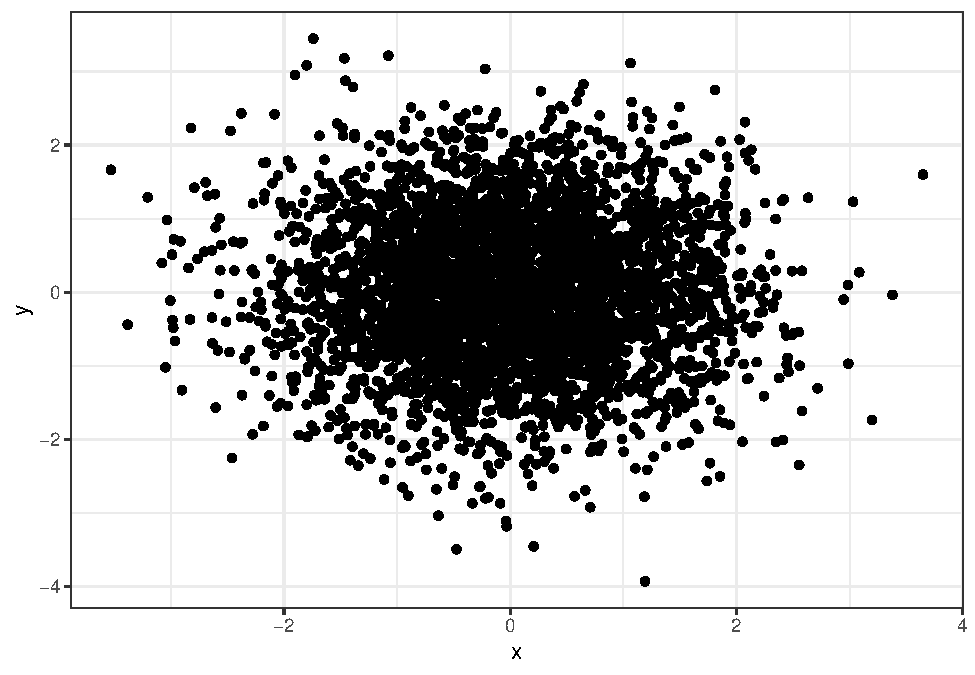
\includegraphics{_main_files/figure-latex/unnamed-chunk-48-1.pdf}

Nasze dane mogą też zawierać wysokości słupków. W takim wypadku należy użyć \texttt{geom\_col}

\begin{Shaded}
\begin{Highlighting}[]
\NormalTok{x }\OtherTok{\textless{}{-}} \FunctionTok{data.frame}\NormalTok{(}\AttributeTok{x =} \FunctionTok{c}\NormalTok{(}\DecValTok{2}\NormalTok{, }\DecValTok{6}\NormalTok{, }\DecValTok{3}\NormalTok{, }\DecValTok{8}\NormalTok{, }\DecValTok{9}\NormalTok{), }\AttributeTok{name =} \FunctionTok{c}\NormalTok{(}\StringTok{"A"}\NormalTok{, }\StringTok{"B"}\NormalTok{, }\StringTok{"C"}\NormalTok{, }\StringTok{"D"}\NormalTok{, }\StringTok{"E"}\NormalTok{))}

\NormalTok{p }\OtherTok{\textless{}{-}} \FunctionTok{ggplot}\NormalTok{(}\AttributeTok{data =}\NormalTok{ x, }\FunctionTok{aes}\NormalTok{(}\AttributeTok{x =}\NormalTok{ name, }\AttributeTok{y =}\NormalTok{ x))}
\NormalTok{p }\SpecialCharTok{+} \FunctionTok{geom\_col}\NormalTok{(}\FunctionTok{aes}\NormalTok{(}\AttributeTok{fill =}\NormalTok{ name))}
\end{Highlighting}
\end{Shaded}

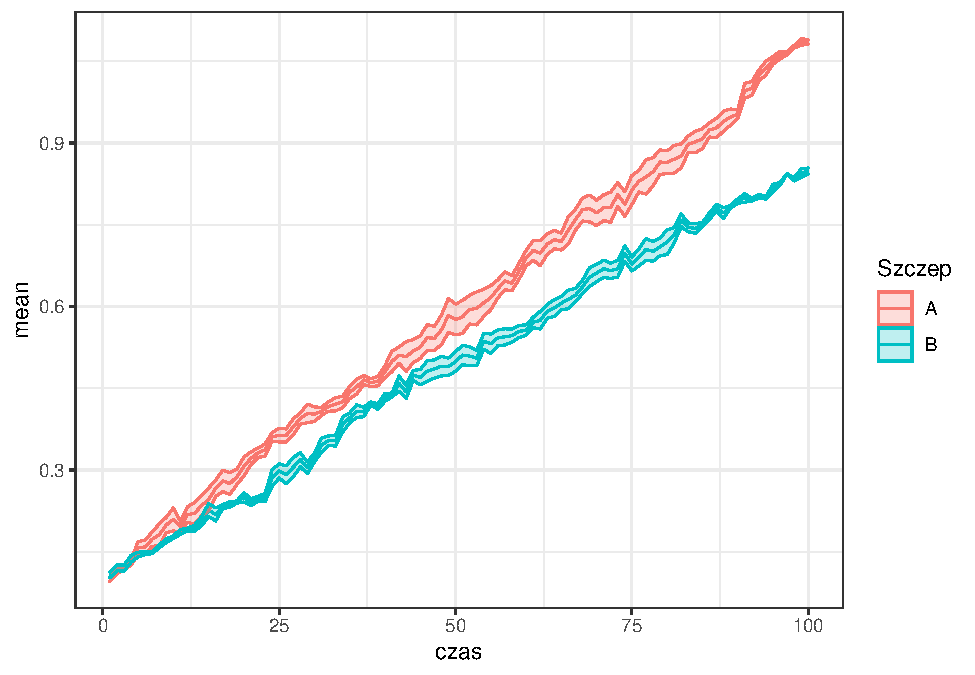
\includegraphics{_main_files/figure-latex/unnamed-chunk-49-1.pdf}

\hypertarget{ux15brednia-mediana-itp.-na-wykresie}{%
\section{Średnia, mediana itp. na wykresie}\label{ux15brednia-mediana-itp.-na-wykresie}}

\hypertarget{stat_summary}{%
\subsection{Stat\_summary}\label{stat_summary}}

Możemy również potrzebować wykres z zaznaczoną średnią i przedziałem ufności albo błędem standardowym.

W takim wypadku możemy sami policzyć te wartości, a następnie pokazać je używając \texttt{geom\_pointrange} albo \texttt{geom\_crossbar}.

Można też wykorzystać \texttt{stat\_summary}, który policzy je za nas.

W \texttt{stat\_summary} najważniejszym argumentem jest funkcja jaką zastosujemy do podsumowania danych. Może to być albo fun.y - należy podać funckję, której wynikiem jest jedna wartość np. \texttt{mean}, \texttt{median}, \texttt{sd} albo fun.data - należy podać funkcję, której wynikiem jest więcej wartości np. \texttt{mean\_cl\_boot} i \texttt{mean\_cl\_normal} policzą średnią i przedział ufności. Należy też dobrać odpowiedni geom: dla jednej wartości np. point albo line, dla większej: linerange, crossbar, pointrange, errorbar.

\begin{Shaded}
\begin{Highlighting}[]
\NormalTok{p }\OtherTok{\textless{}{-}} \FunctionTok{ggplot}\NormalTok{(}\AttributeTok{data=}\NormalTok{dane1, }\FunctionTok{aes}\NormalTok{(}\AttributeTok{x=}\NormalTok{Szczep, }\AttributeTok{y=}\NormalTok{pomiar, }\AttributeTok{color=}\NormalTok{Szczep))}
\CommentTok{\# Wykres tylko z wartością średnią}
\NormalTok{p }\SpecialCharTok{+} \FunctionTok{stat\_summary}\NormalTok{(}\AttributeTok{fun =} \StringTok{"mean"}\NormalTok{, }\AttributeTok{geom =} \StringTok{"point"}\NormalTok{, }\AttributeTok{size =} \DecValTok{3}\NormalTok{)}\SpecialCharTok{+}
  \FunctionTok{facet\_wrap}\NormalTok{(}\SpecialCharTok{\textasciitilde{}}\NormalTok{ warunki, }\AttributeTok{ncol =} \DecValTok{2}\NormalTok{)}
\end{Highlighting}
\end{Shaded}

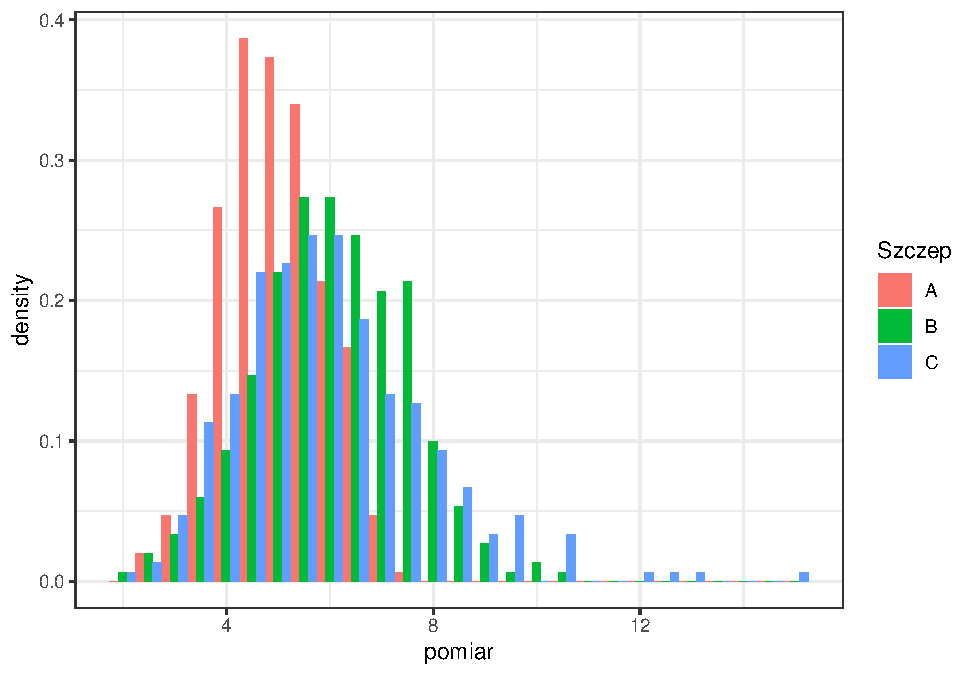
\includegraphics{_main_files/figure-latex/unnamed-chunk-50-1.pdf}

\begin{Shaded}
\begin{Highlighting}[]
\CommentTok{\# Wykres ze średnią i przedziałem ufności policzonym metodą bootstrap}
\NormalTok{p }\SpecialCharTok{+} \FunctionTok{stat\_summary}\NormalTok{(}\AttributeTok{fun.data =} \StringTok{"mean\_cl\_boot"}\NormalTok{)}\SpecialCharTok{+}
  \FunctionTok{facet\_wrap}\NormalTok{(}\SpecialCharTok{\textasciitilde{}}\NormalTok{ warunki, }\AttributeTok{ncol =} \DecValTok{2}\NormalTok{)}
\end{Highlighting}
\end{Shaded}

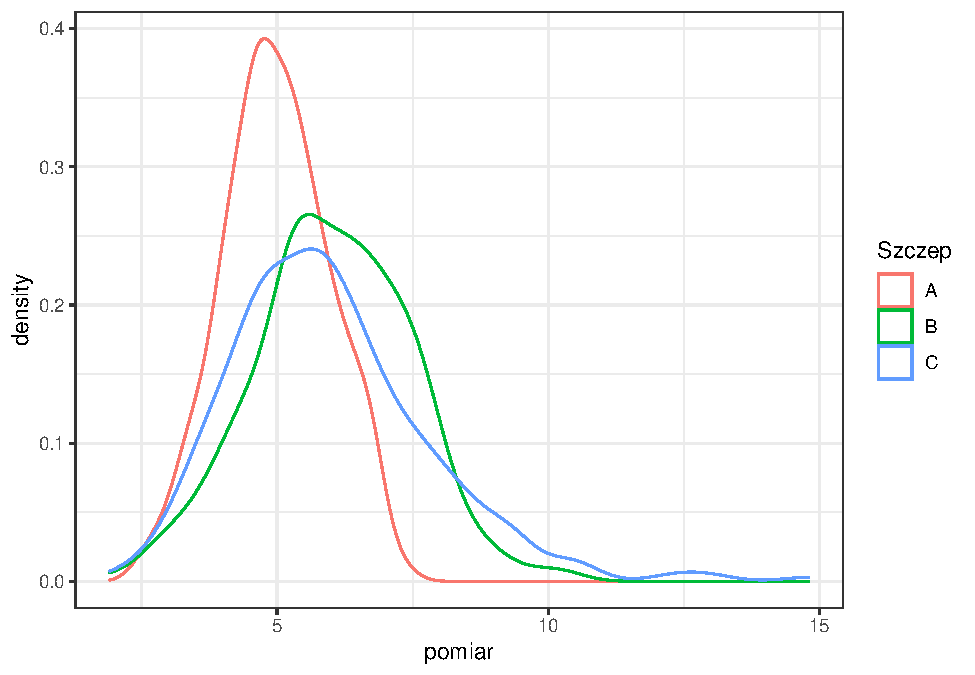
\includegraphics{_main_files/figure-latex/unnamed-chunk-50-2.pdf}

\hypertarget{summary-z-uux17cyciem-dplyr}{%
\subsection{Summary z użyciem dplyr}\label{summary-z-uux17cyciem-dplyr}}

Do samodzielnego policzenia średnich możemy wykorzystać pakiet dplyr. Pozwala on m.in. na szybkie tworzenie podsumowań danych ze względu na zmienne np. różne szczepy.

Najpierw dane są dzielone na grupy, następnie każda grupa jest poddawana działaniu pewnej funkcji lub kilku funkcji, a wynik jest zapisywany do nowej ramki danych.

W pakiecie dplyr pierwszym krokiem jest podział na grupy - \texttt{group\_by} i potem przekazania wyniku do funkcji \texttt{summarize}.

\begin{Shaded}
\begin{Highlighting}[]
\FunctionTok{library}\NormalTok{(dplyr)}

\NormalTok{summ }\OtherTok{\textless{}{-}}\NormalTok{ dane1 }\SpecialCharTok{\%\textgreater{}\%} \FunctionTok{group\_by}\NormalTok{(Szczep, warunki) }\SpecialCharTok{\%\textgreater{}\%} 
  \FunctionTok{summarize}\NormalTok{(}\AttributeTok{mean =} \FunctionTok{mean}\NormalTok{(pomiar), }\AttributeTok{odch =} \FunctionTok{sd}\NormalTok{(pomiar), }
            \AttributeTok{blad =}\NormalTok{ odch}\SpecialCharTok{/}\FunctionTok{sqrt}\NormalTok{(}\FunctionTok{length}\NormalTok{(pomiar)),}
            \AttributeTok{lower =}\NormalTok{ mean}\SpecialCharTok{{-}}\NormalTok{blad, }
            \AttributeTok{upper =}\NormalTok{ mean}\SpecialCharTok{+}\NormalTok{blad)}
\end{Highlighting}
\end{Shaded}

\begin{verbatim}
## `summarise()` has grouped output by 'Szczep'. You can override using the `.groups` argument.
\end{verbatim}

\begin{Shaded}
\begin{Highlighting}[]
\NormalTok{summ}
\end{Highlighting}
\end{Shaded}

\begin{verbatim}
## # A tibble: 6 x 7
## # Groups:   Szczep [3]
##   Szczep warunki  mean  odch   blad lower upper
##   <chr>    <int> <dbl> <dbl>  <dbl> <dbl> <dbl>
## 1 A            1  4.98 0.973 0.0562  4.93  5.04
## 2 A            2  3.96 0.748 0.0432  3.92  4.00
## 3 B            1  6.02 1.43  0.0828  5.93  6.10
## 4 B            2  6.07 1.13  0.0654  6.00  6.13
## 5 C            1  5.96 1.85  0.107   5.85  6.07
## 6 C            2  8.08 3.40  0.196   7.89  8.28
\end{verbatim}

\begin{Shaded}
\begin{Highlighting}[]
\NormalTok{p }\OtherTok{\textless{}{-}} \FunctionTok{ggplot}\NormalTok{(}\AttributeTok{data =}\NormalTok{ summ, }\FunctionTok{aes}\NormalTok{(}\AttributeTok{x =}\NormalTok{ Szczep, }\AttributeTok{y =}\NormalTok{ mean, }\AttributeTok{ymin =}\NormalTok{ lower, }\AttributeTok{ymax =}\NormalTok{ upper, }
                             \AttributeTok{color =}\NormalTok{ Szczep)) }\SpecialCharTok{+} \FunctionTok{facet\_wrap}\NormalTok{(}\SpecialCharTok{\textasciitilde{}}\NormalTok{ warunki, }\AttributeTok{ncol =} \DecValTok{2}\NormalTok{)}

\CommentTok{\# Wykres ze średnią i błędem standardowym}
\NormalTok{p }\SpecialCharTok{+} \FunctionTok{geom\_pointrange}\NormalTok{()}
\end{Highlighting}
\end{Shaded}

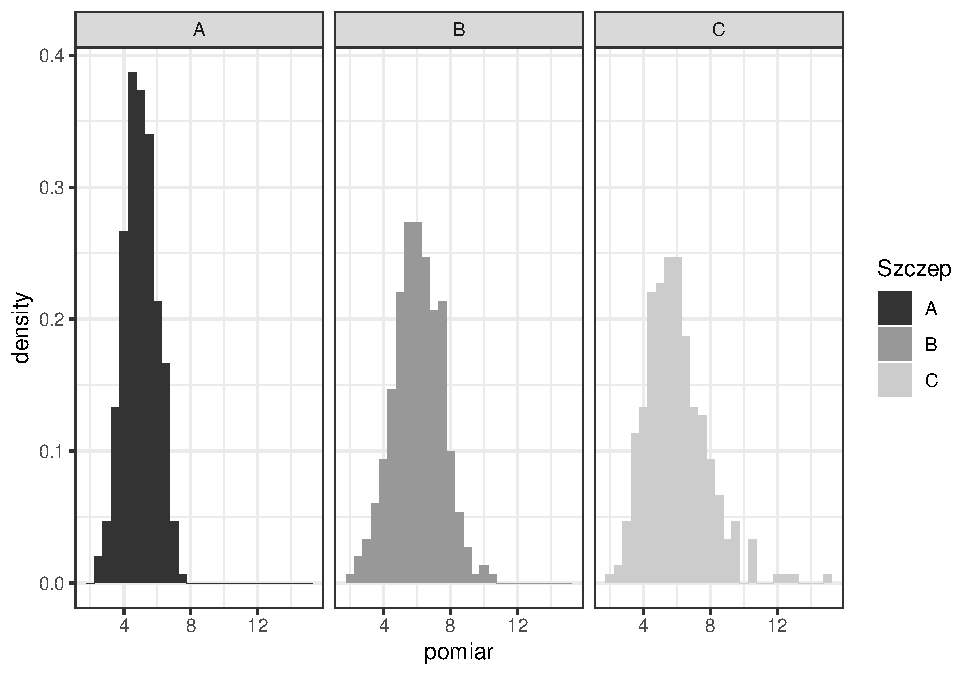
\includegraphics{_main_files/figure-latex/unnamed-chunk-51-1.pdf}

\begin{Shaded}
\begin{Highlighting}[]
\NormalTok{p }\SpecialCharTok{+} \FunctionTok{geom\_crossbar}\NormalTok{(}\AttributeTok{width =} \FloatTok{0.5}\NormalTok{)}
\end{Highlighting}
\end{Shaded}

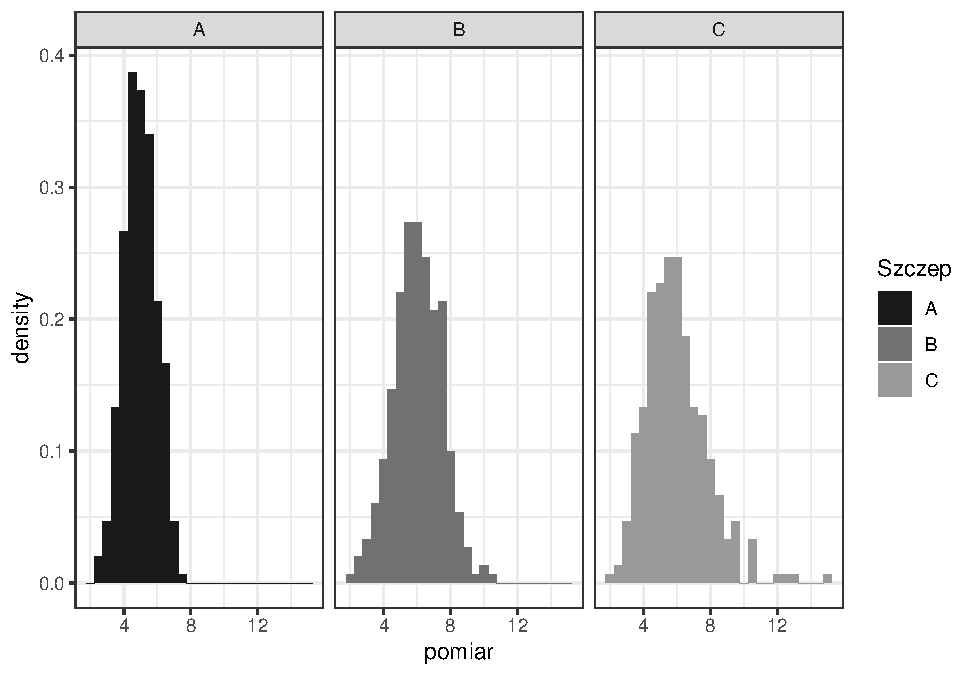
\includegraphics{_main_files/figure-latex/unnamed-chunk-51-2.pdf}

\begin{Shaded}
\begin{Highlighting}[]
\NormalTok{p }\SpecialCharTok{+} \FunctionTok{geom\_errorbar}\NormalTok{(}\AttributeTok{width =} \FloatTok{0.5}\NormalTok{, }\AttributeTok{color =} \StringTok{"black"}\NormalTok{) }\SpecialCharTok{+} \FunctionTok{geom\_point}\NormalTok{()}
\end{Highlighting}
\end{Shaded}

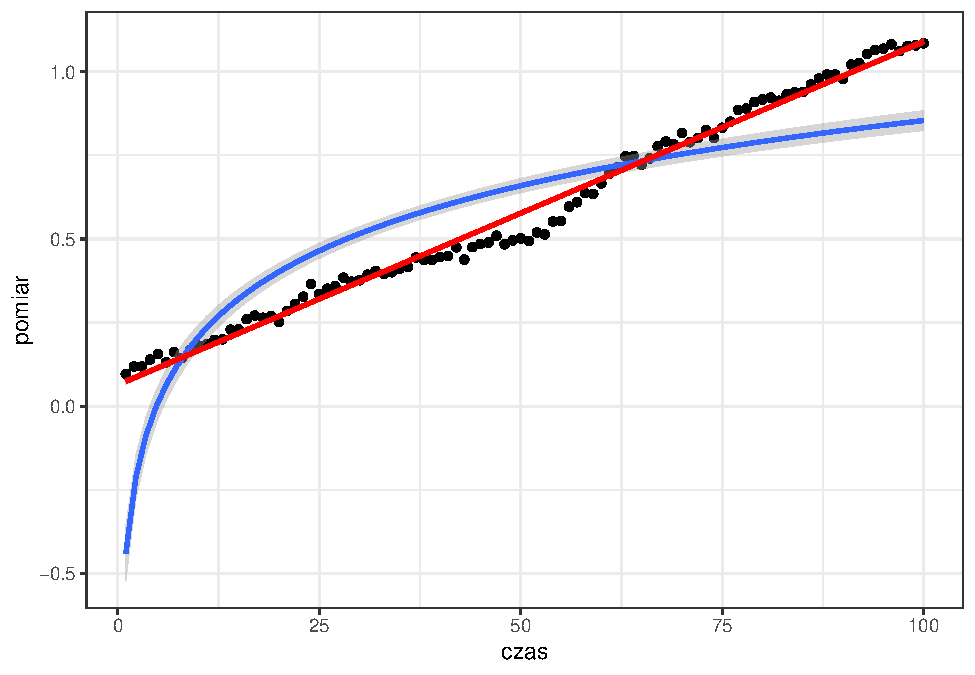
\includegraphics{_main_files/figure-latex/unnamed-chunk-51-3.pdf}

\begin{Shaded}
\begin{Highlighting}[]
\CommentTok{\# Z wykresem przedstawiającym średnie można postąpić tak samo jak z boxplotem}
\NormalTok{p }\OtherTok{\textless{}{-}} \FunctionTok{ggplot}\NormalTok{(}\AttributeTok{data =}\NormalTok{ summ, }\FunctionTok{aes}\NormalTok{(}\AttributeTok{x =}\NormalTok{ Szczep, }\AttributeTok{y =}\NormalTok{ mean, }\AttributeTok{ymin =}\NormalTok{ lower, }\AttributeTok{ymax =}\NormalTok{ upper, }
                             \AttributeTok{color=}\FunctionTok{factor}\NormalTok{(warunki)))}
\NormalTok{p }\SpecialCharTok{+} \FunctionTok{geom\_crossbar}\NormalTok{(}\AttributeTok{width =} \FloatTok{0.5}\NormalTok{, }\AttributeTok{position =} \StringTok{"dodge"}\NormalTok{)}
\end{Highlighting}
\end{Shaded}

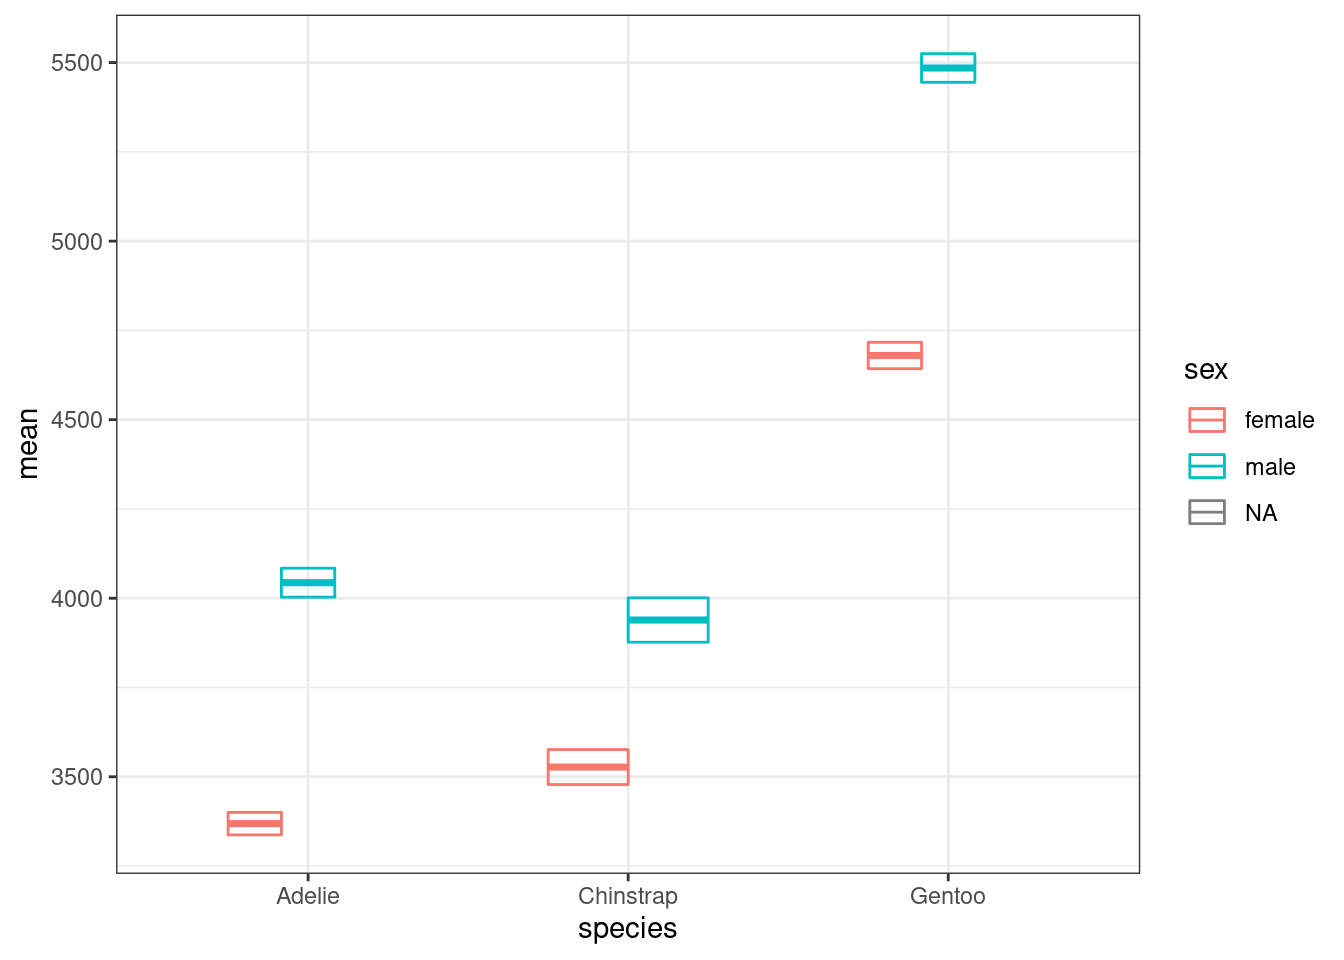
\includegraphics{_main_files/figure-latex/unnamed-chunk-51-4.pdf}

\begin{Shaded}
\begin{Highlighting}[]
\CommentTok{\# Jeżeli średnie połączymy za pomocą linii otrzymamy wykres interakcji opisany w dalszej części}
\NormalTok{p }\OtherTok{\textless{}{-}} \FunctionTok{ggplot}\NormalTok{(}\AttributeTok{data =}\NormalTok{ summ, }\FunctionTok{aes}\NormalTok{(}\AttributeTok{x =}\NormalTok{ Szczep, }\AttributeTok{y =}\NormalTok{ mean, }\AttributeTok{color =} \FunctionTok{factor}\NormalTok{(warunki)))}
\NormalTok{p }\SpecialCharTok{+} \FunctionTok{geom\_point}\NormalTok{() }\SpecialCharTok{+} \FunctionTok{geom\_line}\NormalTok{(}\FunctionTok{aes}\NormalTok{(}\AttributeTok{group =}\NormalTok{ warunki))}
\end{Highlighting}
\end{Shaded}

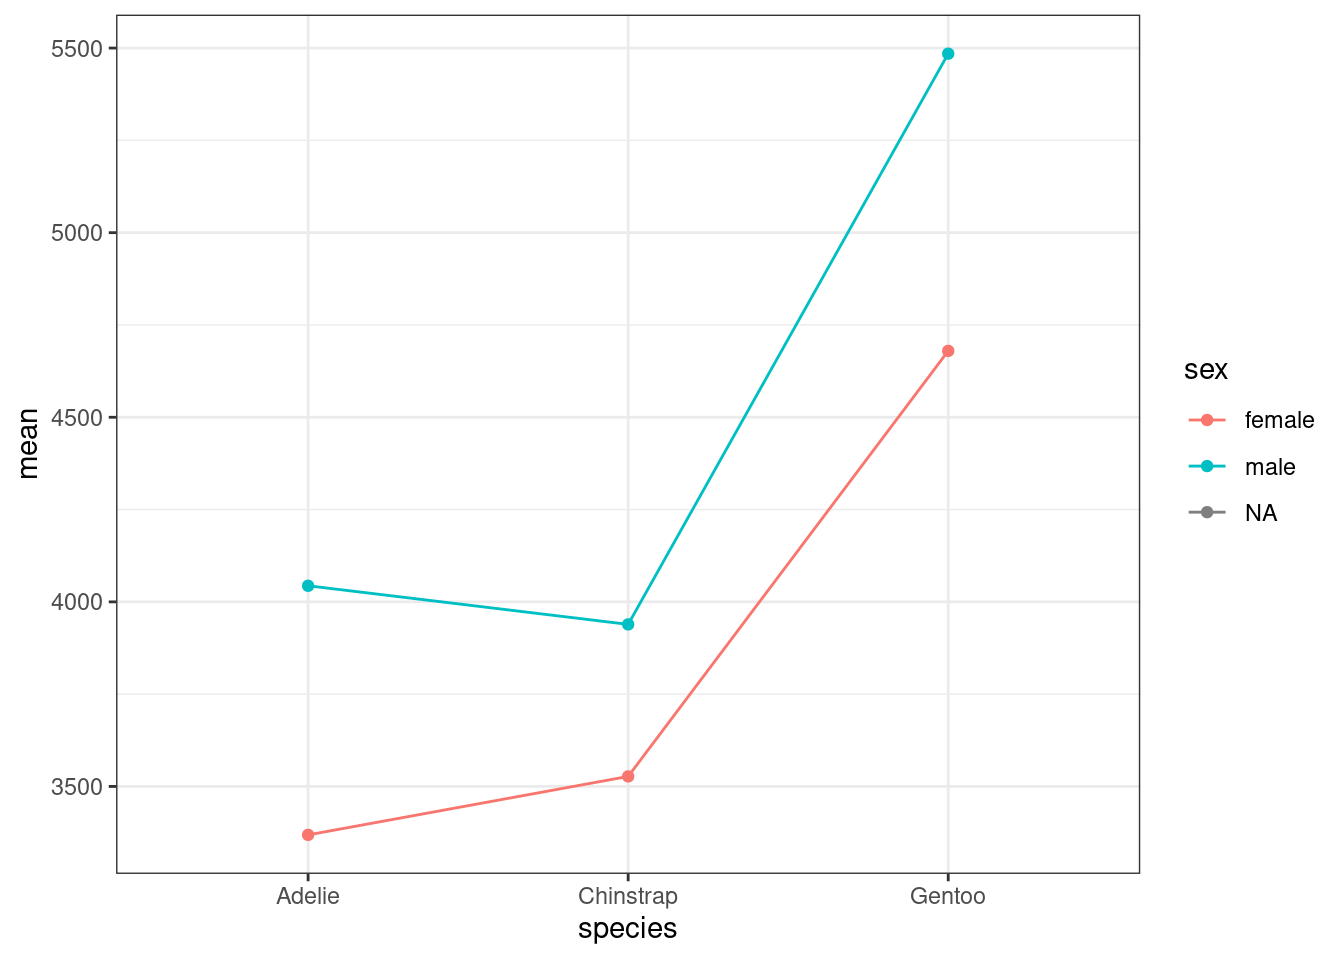
\includegraphics{_main_files/figure-latex/unnamed-chunk-51-5.pdf}

\hypertarget{sux142upki-bux142ux119duxf3w}{%
\subsection{Słupki błędów}\label{sux142upki-bux142ux119duxf3w}}

W publikacja często spotyka się wykresy słupkowe z dodanym słupkiem błędu. Podobny efekt w ggplot2 można uzyskać przy pomocy \texttt{geom\_errorbar} albo \texttt{geom\_linerange}. Należy w \texttt{aes} podać dolną i górną granicę słupka. Jednak jeżeli słupki pochodzą np. z trzech powtórzeń danego eksperymentu to może lepiej byłoby je zaznaczyć w postaci kropek z przedziałem ufności niż rysować słupki.

Wartość średnią i ewentualny błąd standardowy albo przedział ufności możemy policzyć sami albo wykorzystać w tym celu \texttt{stat\_summary}.

\begin{Shaded}
\begin{Highlighting}[]
\CommentTok{\# Przykładowe dane}

\NormalTok{dane }\OtherTok{\textless{}{-}} \FunctionTok{data.frame}\NormalTok{(}\AttributeTok{kontrola =} \FunctionTok{c}\NormalTok{(}\DecValTok{3}\NormalTok{,}\DecValTok{7}\NormalTok{,}\DecValTok{6}\NormalTok{), }\AttributeTok{eksp\_1 =} \FunctionTok{c}\NormalTok{(}\DecValTok{5}\NormalTok{,}\DecValTok{9}\NormalTok{,}\FloatTok{7.5}\NormalTok{), }\AttributeTok{eksp\_2 =} \FunctionTok{c}\NormalTok{(}\DecValTok{3}\NormalTok{,}\DecValTok{1}\NormalTok{,}\DecValTok{6}\NormalTok{), }\AttributeTok{eksp\_3 =} \FunctionTok{c}\NormalTok{(}\DecValTok{10}\NormalTok{,}\DecValTok{11}\NormalTok{,}\DecValTok{8}\NormalTok{), }\AttributeTok{eksp\_4 =} \FunctionTok{c}\NormalTok{(}\DecValTok{1}\NormalTok{,}\DecValTok{12}\NormalTok{,}\DecValTok{4}\NormalTok{))}

\CommentTok{\# przechodzimy do formatu tidy}
\FunctionTok{library}\NormalTok{(tidyr)}

\NormalTok{dane }\SpecialCharTok{\%\textgreater{}\%} \FunctionTok{pivot\_longer}\NormalTok{(}\AttributeTok{cols =} \FunctionTok{everything}\NormalTok{(), }\AttributeTok{names\_to =} \StringTok{\textquotesingle{}key\textquotesingle{}}\NormalTok{, }\AttributeTok{values\_to =} \StringTok{\textquotesingle{}value\textquotesingle{}}\NormalTok{) }\OtherTok{{-}\textgreater{}}\NormalTok{ dane}
\FunctionTok{head}\NormalTok{(dane)}
\end{Highlighting}
\end{Shaded}

\begin{verbatim}
## # A tibble: 6 x 2
##   key      value
##   <chr>    <dbl>
## 1 kontrola     3
## 2 eksp_1       5
## 3 eksp_2       3
## 4 eksp_3      10
## 5 eksp_4       1
## 6 kontrola     7
\end{verbatim}

\begin{Shaded}
\begin{Highlighting}[]
\CommentTok{\# liczymy średnią i np. błąd standardowy}

\NormalTok{podsumowanie }\OtherTok{\textless{}{-}}\NormalTok{ dane }\SpecialCharTok{\%\textgreater{}\%} \FunctionTok{group\_by}\NormalTok{(key) }\SpecialCharTok{\%\textgreater{}\%}
  \FunctionTok{summarize}\NormalTok{(                      }\AttributeTok{srednia =} \FunctionTok{mean}\NormalTok{(value), }
                                  \AttributeTok{odchylenie =} \FunctionTok{sd}\NormalTok{(value), }
                                  \AttributeTok{dolny =}\NormalTok{ srednia}\SpecialCharTok{{-}}\NormalTok{(odchylenie}\SpecialCharTok{/}\FunctionTok{sqrt}\NormalTok{(}\FunctionTok{length}\NormalTok{(value))), }
                                  \AttributeTok{gorny =}\NormalTok{ srednia}\SpecialCharTok{+}\NormalTok{(odchylenie}\SpecialCharTok{/}\FunctionTok{sqrt}\NormalTok{(}\FunctionTok{length}\NormalTok{(value))))}

\CommentTok{\# Wykres słupkowy z zaznaczonym błędem standardowym}
\NormalTok{p }\OtherTok{\textless{}{-}} \FunctionTok{ggplot}\NormalTok{(}\AttributeTok{data =}\NormalTok{ podsumowanie)}
\NormalTok{p }\SpecialCharTok{+} \FunctionTok{geom\_col}\NormalTok{(}\FunctionTok{aes}\NormalTok{(}\AttributeTok{x =}\NormalTok{ key, }\AttributeTok{y =}\NormalTok{ srednia), }\AttributeTok{fill =} \StringTok{"lightblue3"}\NormalTok{)}\SpecialCharTok{+}
  \FunctionTok{geom\_errorbar}\NormalTok{(}\FunctionTok{aes}\NormalTok{(}\AttributeTok{ymin =}\NormalTok{ dolny, }\AttributeTok{ymax =}\NormalTok{ gorny, }\AttributeTok{x =}\NormalTok{ key), }\AttributeTok{width =} \FloatTok{0.2}\NormalTok{)}
\end{Highlighting}
\end{Shaded}

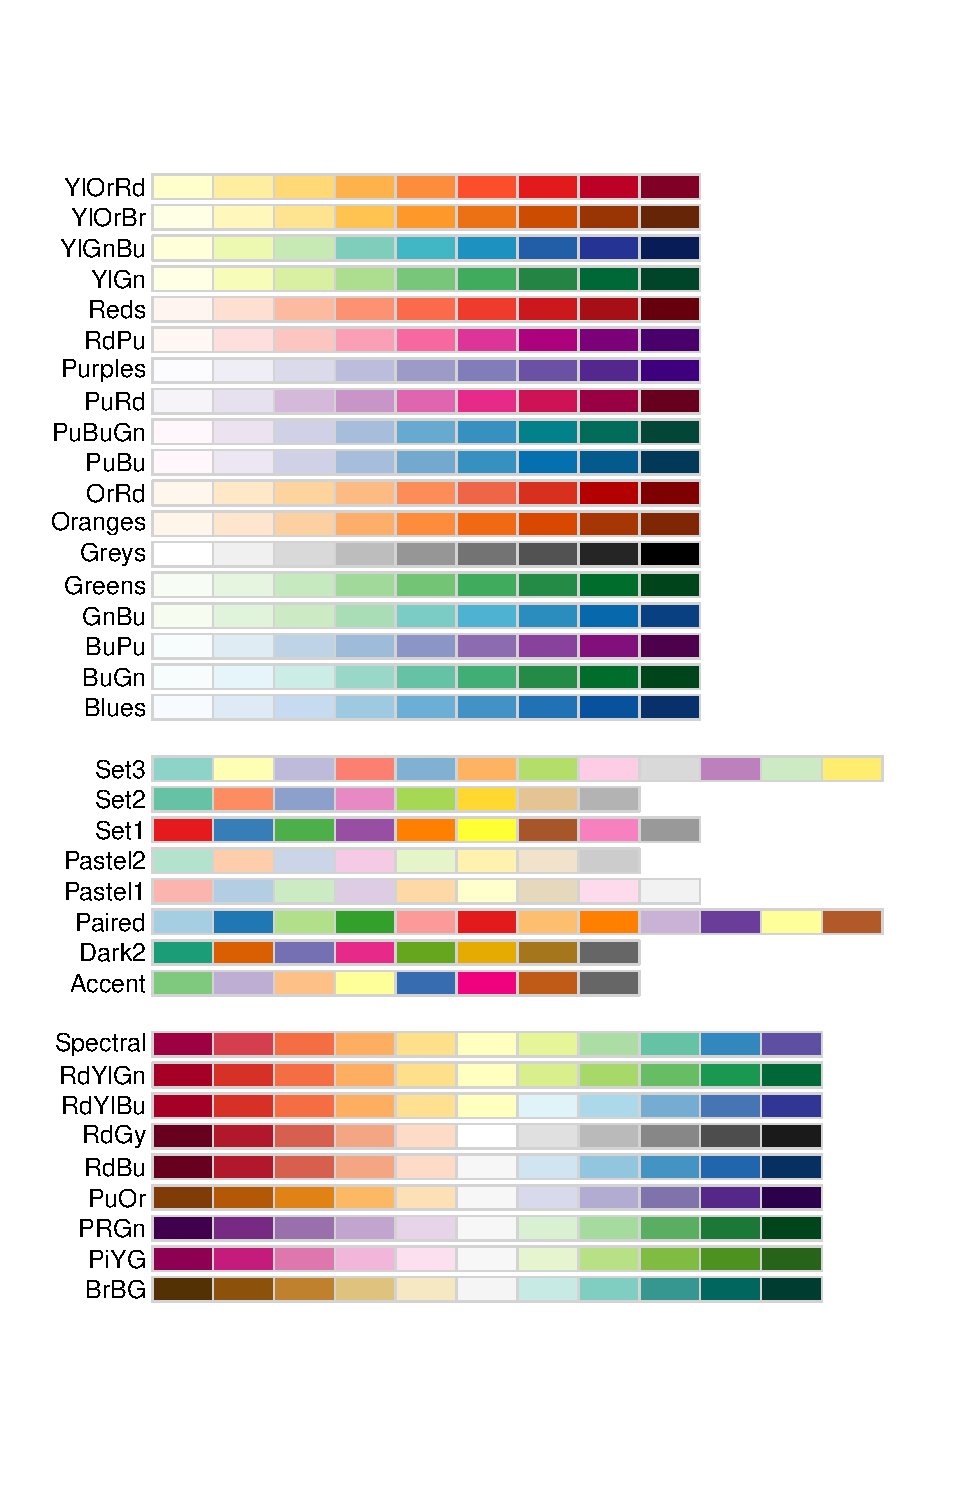
\includegraphics{_main_files/figure-latex/unnamed-chunk-52-1.pdf}

\begin{Shaded}
\begin{Highlighting}[]
\NormalTok{p }\SpecialCharTok{+} \FunctionTok{geom\_col}\NormalTok{(}\FunctionTok{aes}\NormalTok{(}\AttributeTok{x =}\NormalTok{ key, }\AttributeTok{y =}\NormalTok{ srednia), }\AttributeTok{fill =} \StringTok{"lightblue3"}\NormalTok{)}\SpecialCharTok{+}
  \FunctionTok{geom\_linerange}\NormalTok{(}\FunctionTok{aes}\NormalTok{(}\AttributeTok{ymin =}\NormalTok{ dolny, }\AttributeTok{ymax =}\NormalTok{ gorny, }\AttributeTok{x =}\NormalTok{ key))}
\end{Highlighting}
\end{Shaded}

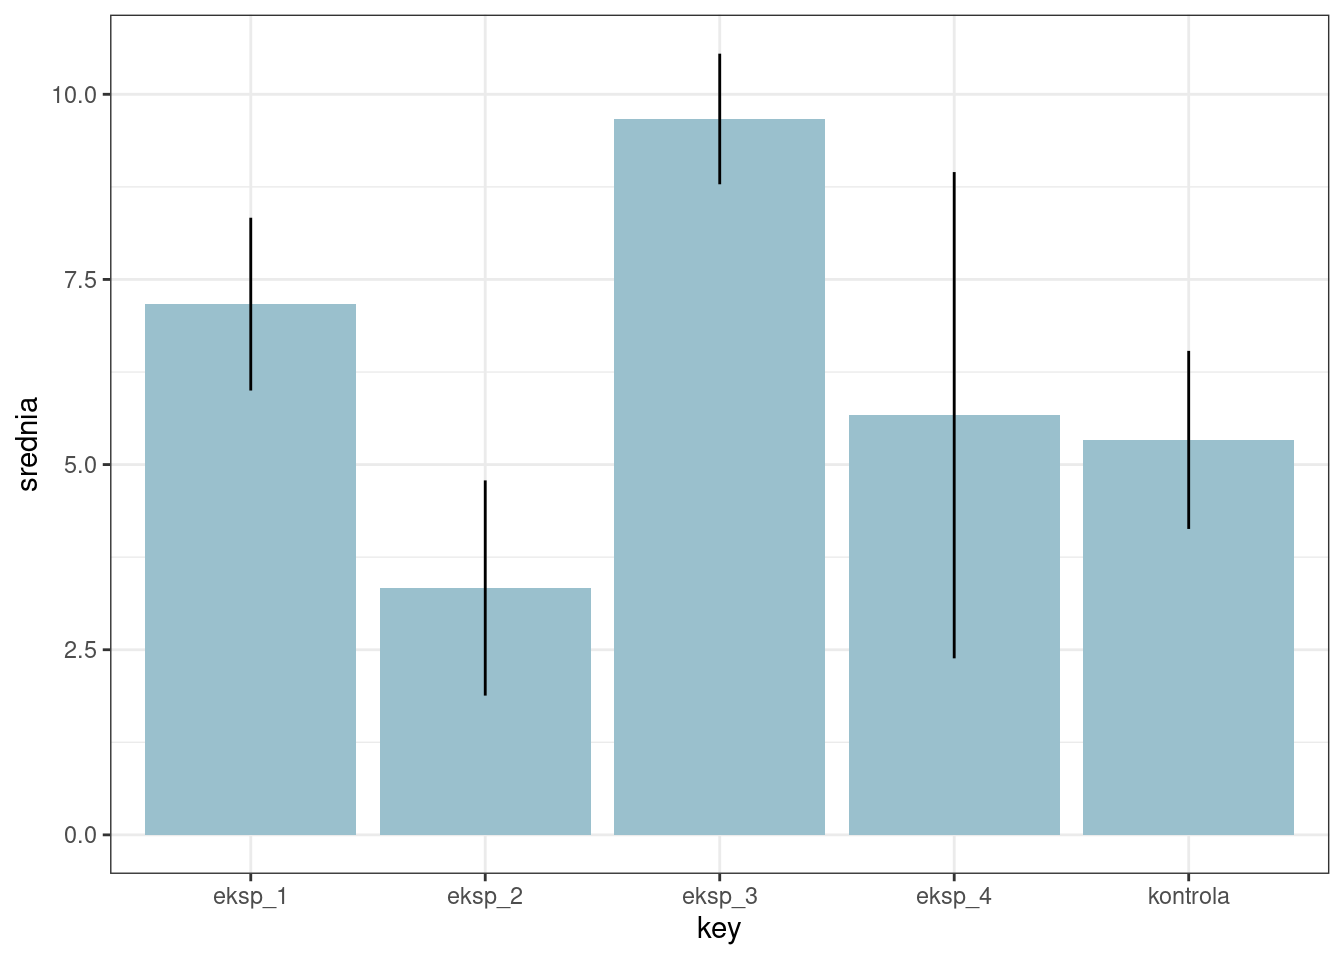
\includegraphics{_main_files/figure-latex/unnamed-chunk-52-2.pdf}

\begin{Shaded}
\begin{Highlighting}[]
\CommentTok{\# Wykres punktowy wyników z zaznaczonym błędem standardowym}
\NormalTok{p }\SpecialCharTok{+} \FunctionTok{geom\_point}\NormalTok{(}\AttributeTok{data =}\NormalTok{ dane, }\FunctionTok{aes}\NormalTok{(}\AttributeTok{x =}\NormalTok{ key, }\AttributeTok{y =}\NormalTok{ value))}\SpecialCharTok{+}
  \FunctionTok{geom\_pointrange}\NormalTok{(}\FunctionTok{aes}\NormalTok{(}\AttributeTok{x =}\NormalTok{ key, }\AttributeTok{ymin =}\NormalTok{ dolny, }\AttributeTok{ymax =}\NormalTok{ gorny, }\AttributeTok{y =}\NormalTok{ srednia), }\AttributeTok{col =} \StringTok{"red2"}\NormalTok{)}
\end{Highlighting}
\end{Shaded}

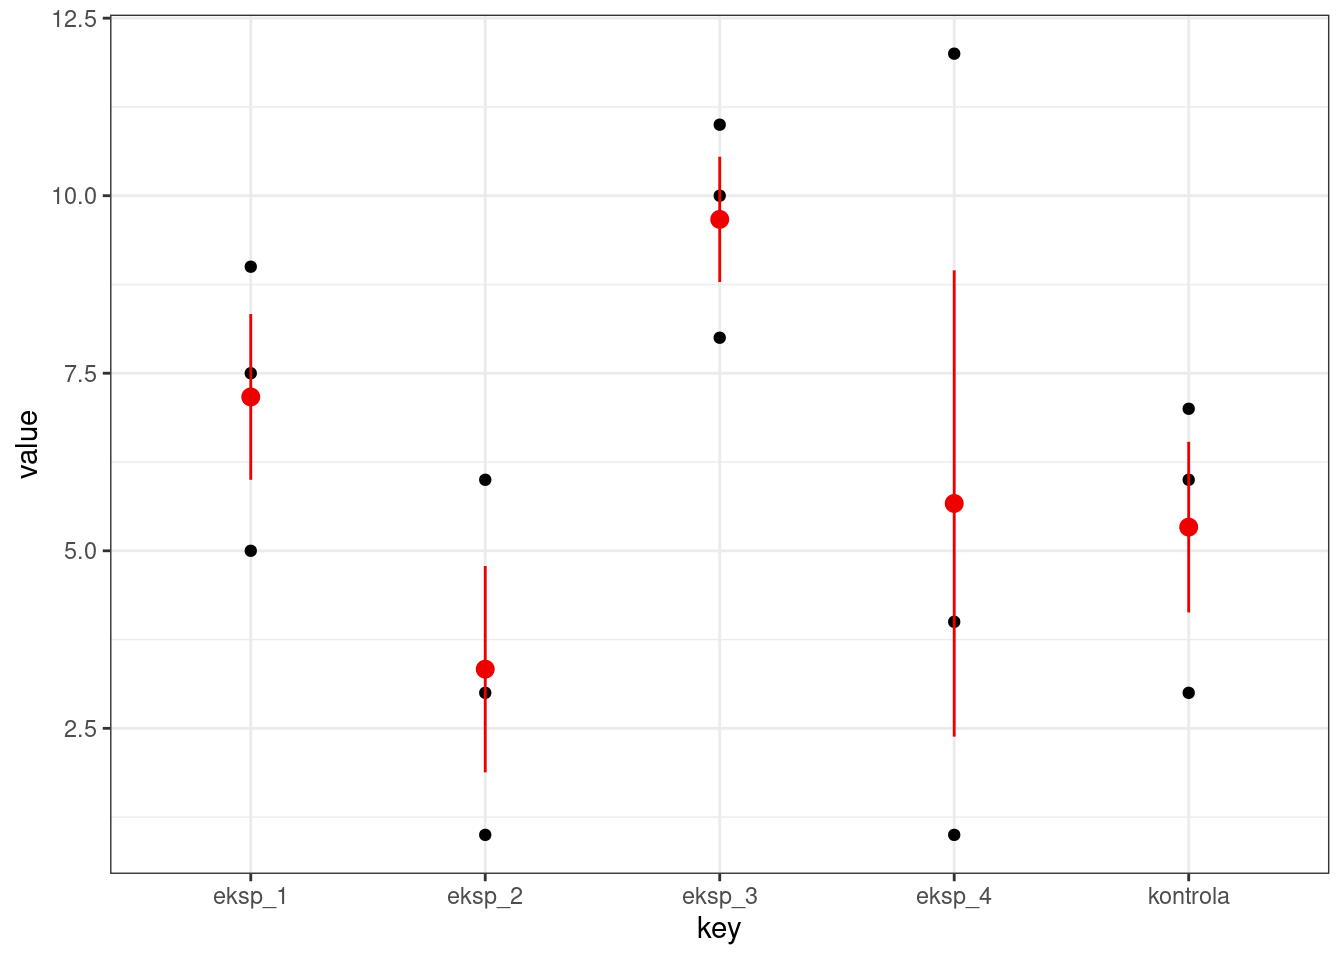
\includegraphics{_main_files/figure-latex/unnamed-chunk-52-3.pdf}

\begin{Shaded}
\begin{Highlighting}[]
\NormalTok{p }\SpecialCharTok{+} \FunctionTok{geom\_point}\NormalTok{(}\AttributeTok{data =}\NormalTok{ dane, }\FunctionTok{aes}\NormalTok{(}\AttributeTok{x =}\NormalTok{ key, }\AttributeTok{y =}\NormalTok{ value))}\SpecialCharTok{+}
  \FunctionTok{geom\_crossbar}\NormalTok{(}\FunctionTok{aes}\NormalTok{(}\AttributeTok{x =}\NormalTok{ key, }\AttributeTok{ymin =}\NormalTok{ dolny, }\AttributeTok{ymax =}\NormalTok{ gorny, }\AttributeTok{y =}\NormalTok{ srednia), }\AttributeTok{col =} \StringTok{"red2"}\NormalTok{, }\AttributeTok{width =} \FloatTok{0.25}\NormalTok{)}
\end{Highlighting}
\end{Shaded}

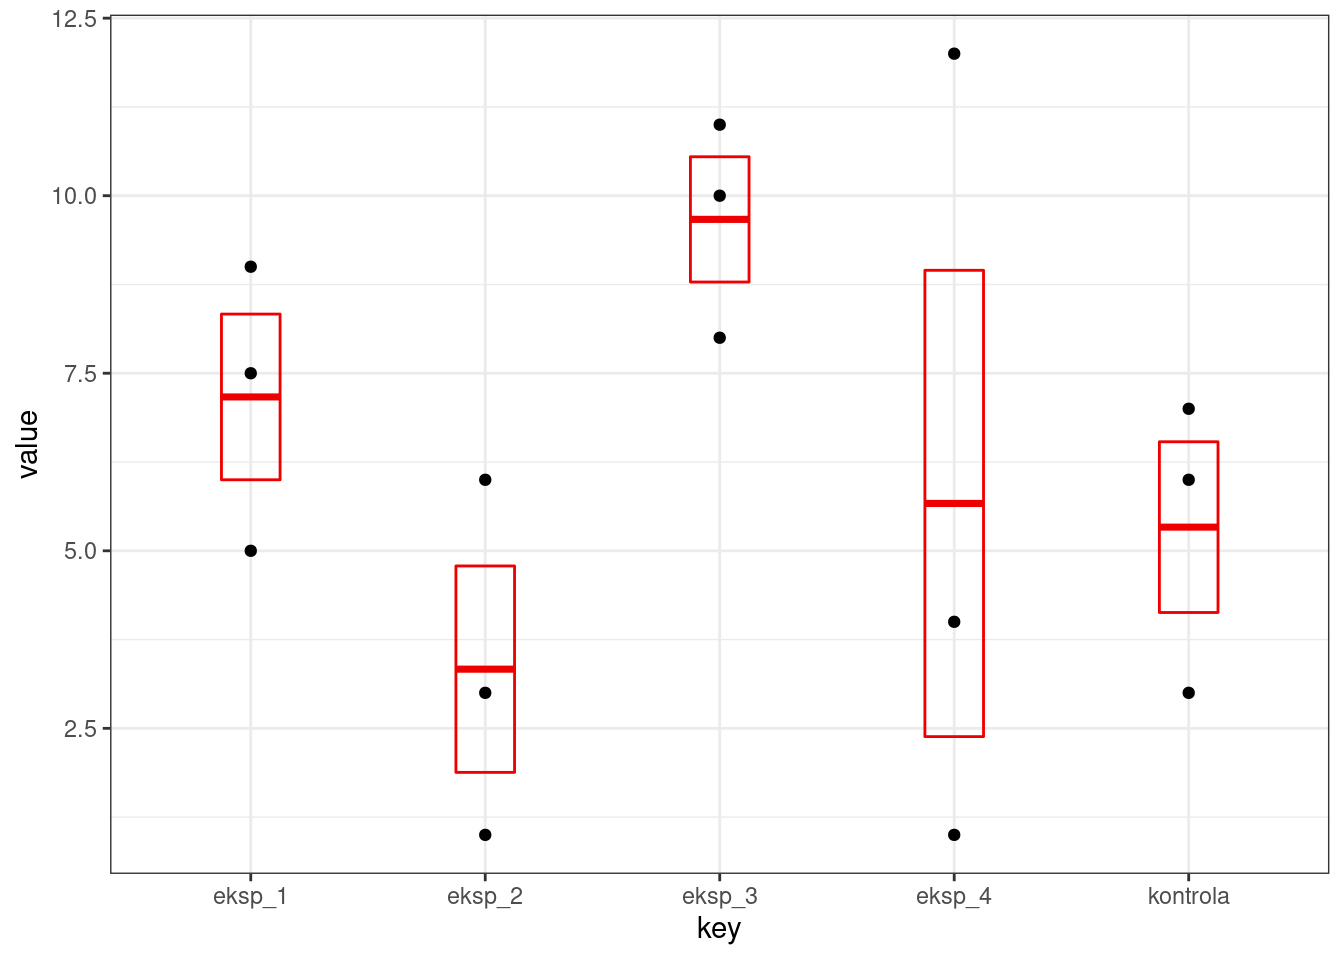
\includegraphics{_main_files/figure-latex/unnamed-chunk-52-4.pdf}

\begin{Shaded}
\begin{Highlighting}[]
\NormalTok{p }\SpecialCharTok{+} \FunctionTok{geom\_point}\NormalTok{(}\AttributeTok{data =}\NormalTok{ dane, }\FunctionTok{aes}\NormalTok{(}\AttributeTok{x =}\NormalTok{ key, }\AttributeTok{y =}\NormalTok{ value))}\SpecialCharTok{+}
  \FunctionTok{geom\_errorbar}\NormalTok{(}\FunctionTok{aes}\NormalTok{(}\AttributeTok{x =}\NormalTok{ key, }\AttributeTok{ymin =}\NormalTok{ dolny, }\AttributeTok{ymax =}\NormalTok{ gorny, }\AttributeTok{y =}\NormalTok{ srednia), }\AttributeTok{col =} \StringTok{"red2"}\NormalTok{, }\AttributeTok{width =} \FloatTok{0.25}\NormalTok{)}
\end{Highlighting}
\end{Shaded}

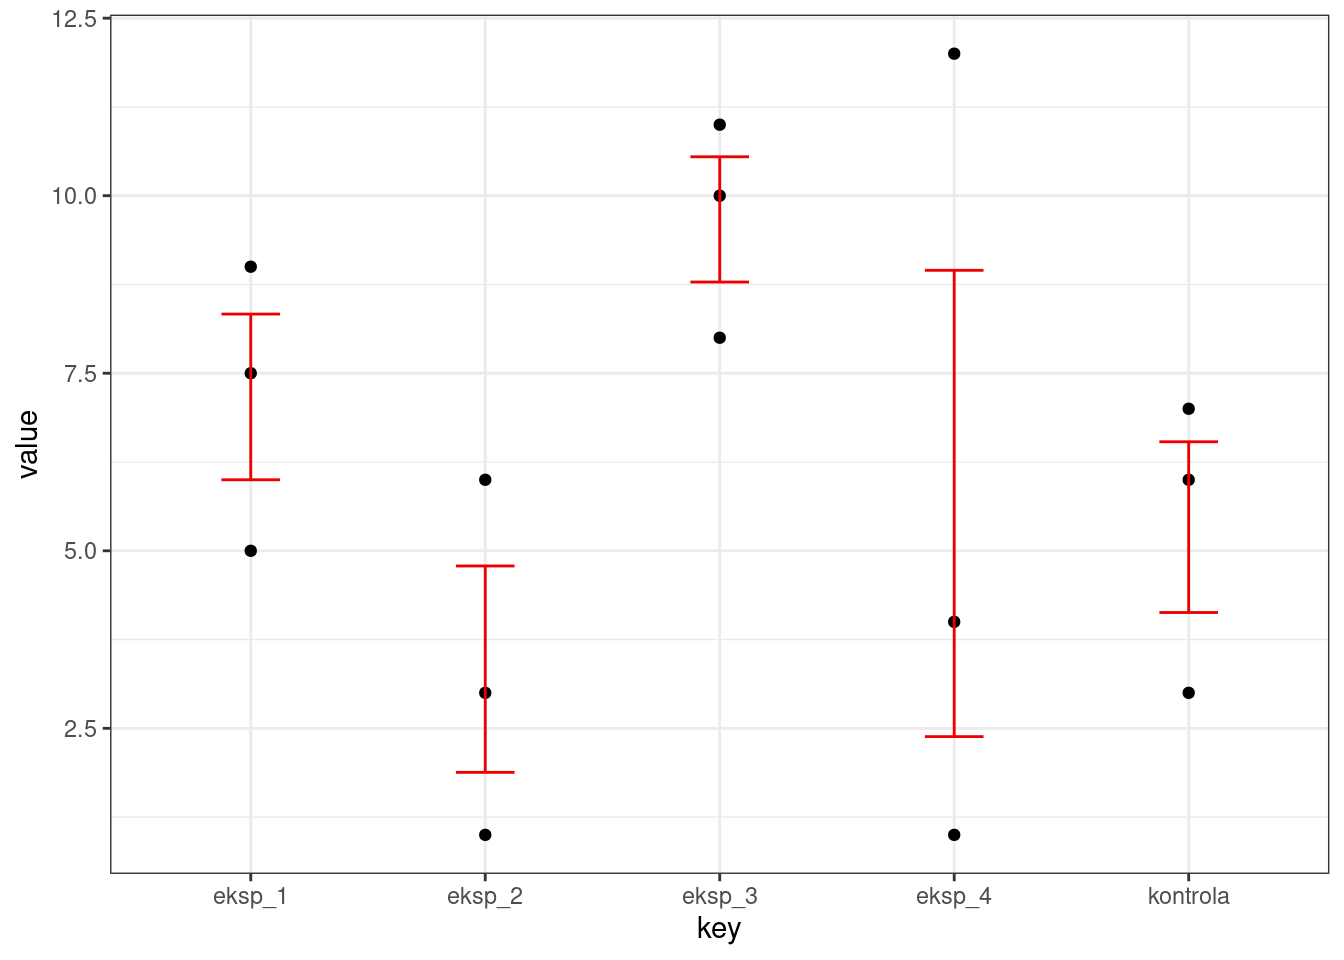
\includegraphics{_main_files/figure-latex/unnamed-chunk-52-5.pdf}

\hypertarget{wykres-punktowy-i-liniowy}{%
\section{Wykres punktowy i liniowy}\label{wykres-punktowy-i-liniowy}}

Zacznijmy od pojedynczego pomiaru szczepu A z dane3

Dla \texttt{geom\_point} albo \texttt{geom\_line} konieczne jest w aes podanie x i y.

\begin{Shaded}
\begin{Highlighting}[]
\NormalTok{dane3\_1 }\OtherTok{\textless{}{-}} \FunctionTok{filter}\NormalTok{(dane3, Szczep }\SpecialCharTok{==} \StringTok{"A"}\NormalTok{ , powt }\SpecialCharTok{==} \StringTok{"1"}\NormalTok{)}

\NormalTok{p }\OtherTok{\textless{}{-}} \FunctionTok{ggplot}\NormalTok{(}\AttributeTok{data =}\NormalTok{ dane3\_1, }\FunctionTok{aes}\NormalTok{(}\AttributeTok{x =}\NormalTok{ czas, }\AttributeTok{y =}\NormalTok{ pomiar))}
\NormalTok{p }\SpecialCharTok{+} \FunctionTok{geom\_point}\NormalTok{()}
\end{Highlighting}
\end{Shaded}

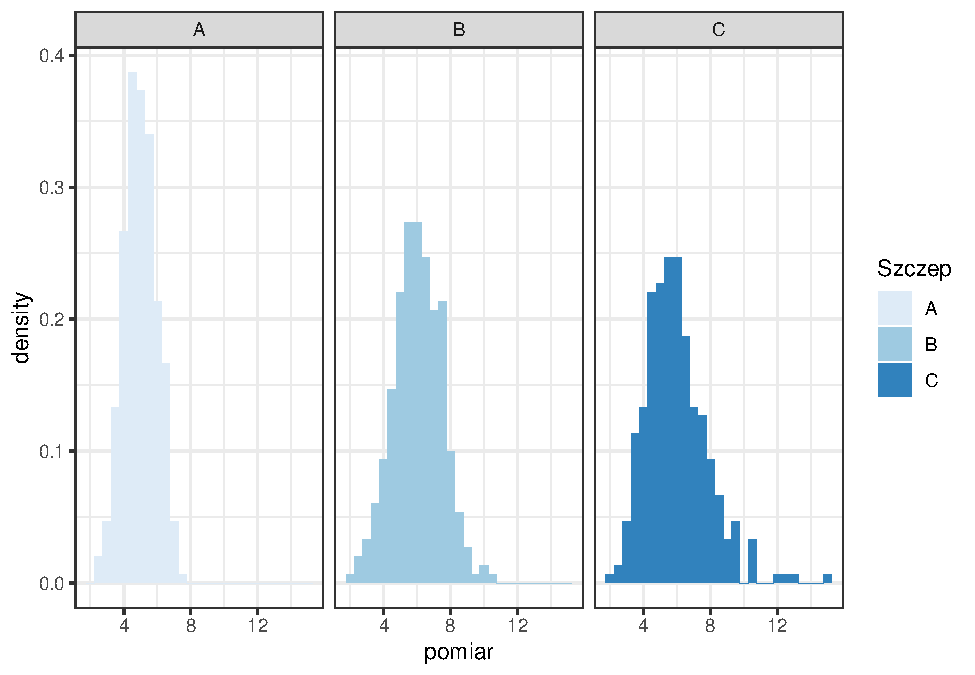
\includegraphics{_main_files/figure-latex/unnamed-chunk-53-1.pdf}

\begin{Shaded}
\begin{Highlighting}[]
\NormalTok{p }\SpecialCharTok{+} \FunctionTok{geom\_line}\NormalTok{()}
\end{Highlighting}
\end{Shaded}

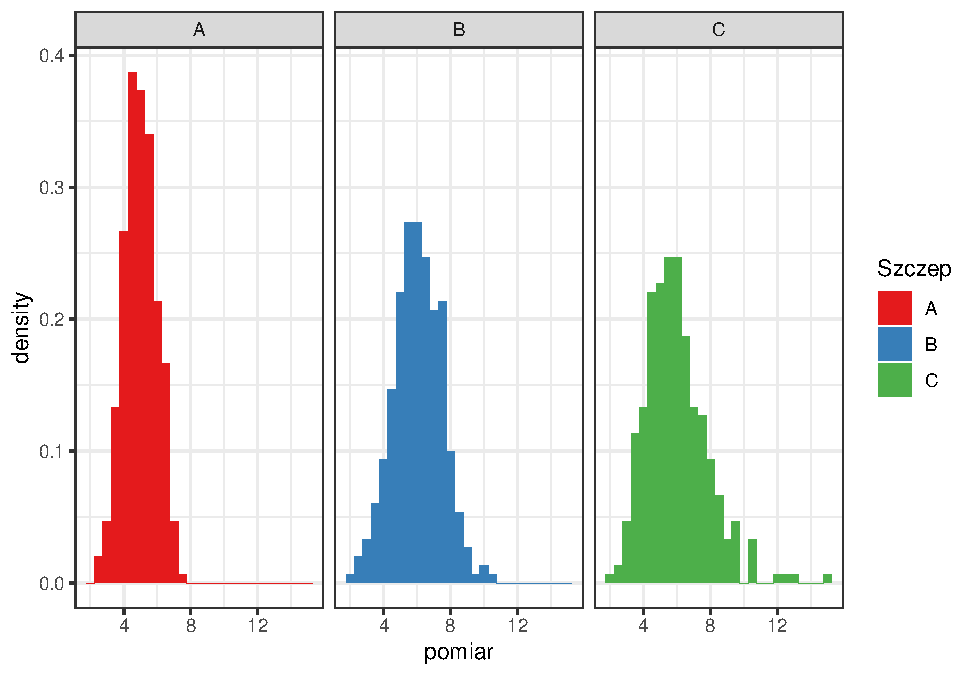
\includegraphics{_main_files/figure-latex/unnamed-chunk-53-2.pdf}

\hypertarget{dopasowanie-linii-trendu-do-wykresu-punktowego}{%
\subsection{Dopasowanie linii trendu do wykresu punktowego}\label{dopasowanie-linii-trendu-do-wykresu-punktowego}}

Zamiast rysować linię, możemy dopasować do wyników linię trendu (może być też inna niż liniowa np. logarytmiczna, kwadratowa, ograniczają nas tylko umiejętności pisania formuł w R ;)). Dopasowanie wykona \texttt{stat\_smooth}. Domyślnie dopasuje linię do danych korzystając z własnego algorytmu (loess - lokalne wygładzanie wielomianami niskich stopni ;)), który ma za zadanie uzyskać jak najlepsze dopasowanie do danych, zaznaczy również przedział ufności. Możemy narzucić własną metodę i formułę.

\begin{Shaded}
\begin{Highlighting}[]
\CommentTok{\# metoda loess}
\NormalTok{p }\SpecialCharTok{+} \FunctionTok{geom\_point}\NormalTok{() }\SpecialCharTok{+} \FunctionTok{stat\_smooth}\NormalTok{()}
\end{Highlighting}
\end{Shaded}

\begin{verbatim}
## `geom_smooth()` using method = 'loess' and formula 'y ~ x'
\end{verbatim}

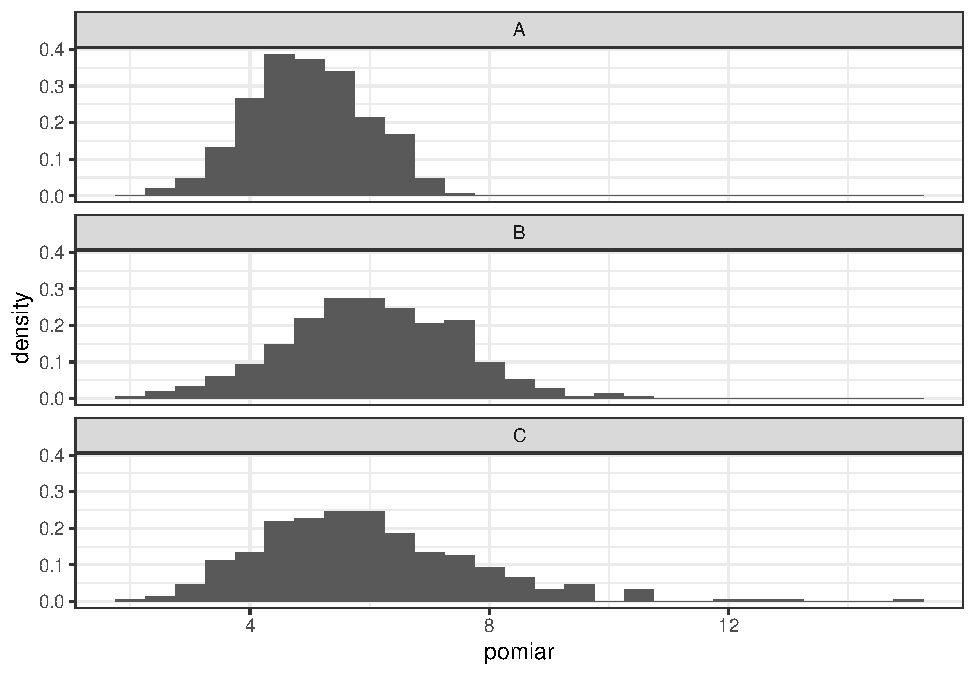
\includegraphics{_main_files/figure-latex/unnamed-chunk-54-1.pdf}

\begin{Shaded}
\begin{Highlighting}[]
\CommentTok{\# metoda lm {-} dopasowanie do linii prostej}
\NormalTok{p }\SpecialCharTok{+} \FunctionTok{geom\_point}\NormalTok{() }\SpecialCharTok{+} \FunctionTok{stat\_smooth}\NormalTok{(}\AttributeTok{method =} \StringTok{"lm"}\NormalTok{)}
\end{Highlighting}
\end{Shaded}

\begin{verbatim}
## `geom_smooth()` using formula 'y ~ x'
\end{verbatim}

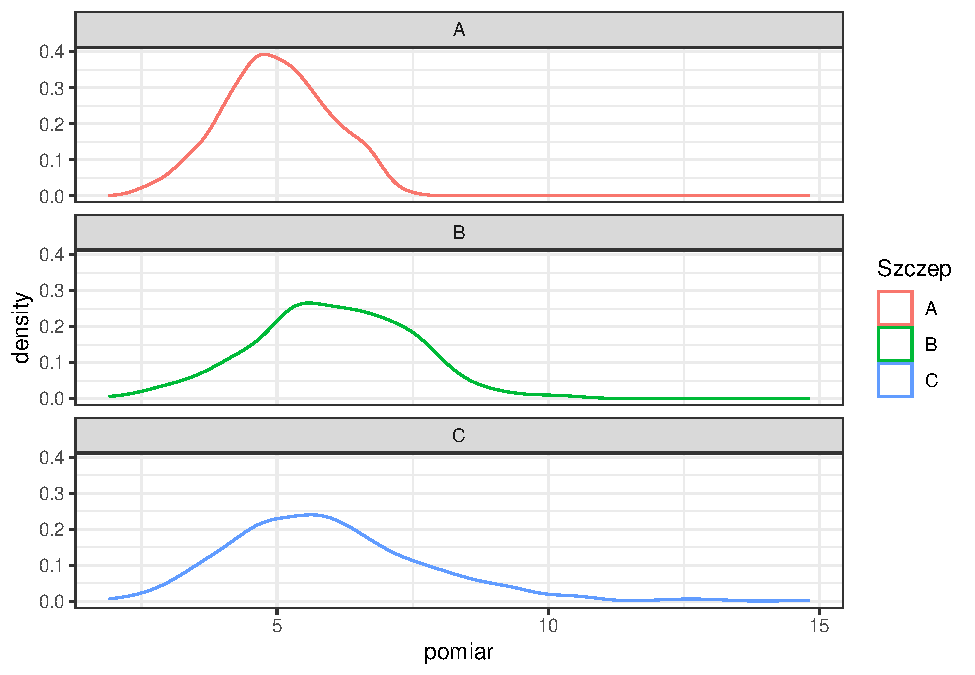
\includegraphics{_main_files/figure-latex/unnamed-chunk-54-2.pdf}

\begin{Shaded}
\begin{Highlighting}[]
\CommentTok{\# metoda lm z podaną formułą}
\NormalTok{p }\SpecialCharTok{+} \FunctionTok{geom\_point}\NormalTok{() }\SpecialCharTok{+} \FunctionTok{stat\_smooth}\NormalTok{(}\AttributeTok{method =} \StringTok{"lm"}\NormalTok{, }\AttributeTok{formula =}\NormalTok{ y}\SpecialCharTok{\textasciitilde{}}\FunctionTok{log}\NormalTok{(x))}\SpecialCharTok{+}
  \FunctionTok{stat\_smooth}\NormalTok{(}\AttributeTok{method =} \StringTok{"lm"}\NormalTok{, }\AttributeTok{color =} \StringTok{"red"}\NormalTok{)}
\end{Highlighting}
\end{Shaded}

\begin{verbatim}
## `geom_smooth()` using formula 'y ~ x'
\end{verbatim}

\includegraphics{_main_files/figure-latex/unnamed-chunk-54-3.pdf}

Sprawdzenie dopasowania można wykonać funkcją \texttt{lm}. Jej \texttt{summary} podaje wartośc R\^{}2, istotność, parametry wzoru(coefficients).

\begin{Shaded}
\begin{Highlighting}[]
\FunctionTok{summary}\NormalTok{(}\FunctionTok{lm}\NormalTok{(pomiar}\SpecialCharTok{\textasciitilde{}}\NormalTok{czas, }\AttributeTok{data=}\NormalTok{dane3\_1))}
\end{Highlighting}
\end{Shaded}

\begin{verbatim}
## 
## Call:
## lm(formula = pomiar ~ czas, data = dane3_1)
## 
## Residuals:
##       Min        1Q    Median        3Q       Max 
## -0.094113 -0.014337  0.009274  0.023692  0.055815 
## 
## Coefficients:
##              Estimate Std. Error t value Pr(>|t|)    
## (Intercept) 6.352e-02  4.631e-03   13.72   <2e-16 ***
## czas        1.027e-02  7.962e-05  128.97   <2e-16 ***
## ---
## Signif. codes:  0 '***' 0.001 '**' 0.01 '*' 0.05 '.' 0.1 ' ' 1
## 
## Residual standard error: 0.0325 on 198 degrees of freedom
## Multiple R-squared:  0.9882, Adjusted R-squared:  0.9882 
## F-statistic: 1.663e+04 on 1 and 198 DF,  p-value: < 2.2e-16
\end{verbatim}

\begin{Shaded}
\begin{Highlighting}[]
\CommentTok{\# dodanie tekstu do wykresu np. równanie opisujące linię trendu}
\NormalTok{p }\SpecialCharTok{+} \FunctionTok{geom\_point}\NormalTok{() }\SpecialCharTok{+} \FunctionTok{stat\_smooth}\NormalTok{(}\AttributeTok{method =} \StringTok{"lm"}\NormalTok{, }\AttributeTok{color =} \StringTok{"red"}\NormalTok{)}\SpecialCharTok{+}
  \FunctionTok{geom\_text}\NormalTok{(}\AttributeTok{data =} \ConstantTok{NULL}\NormalTok{, }\AttributeTok{x =} \DecValTok{50}\NormalTok{, }\AttributeTok{y =} \FloatTok{0.2}\NormalTok{, }\AttributeTok{label =} \StringTok{"y = ax + b"}\NormalTok{, }\AttributeTok{size =} \DecValTok{5}\NormalTok{)}
\end{Highlighting}
\end{Shaded}

\begin{verbatim}
## `geom_smooth()` using formula 'y ~ x'
\end{verbatim}

\includegraphics{_main_files/figure-latex/unnamed-chunk-55-1.pdf}

Możemy zastosować \texttt{stat\_smooth} dla wszystkich danych.

\texttt{geom\_point} można rozróżniać pod względem: color, shape, size, a \texttt{geom\_line} pod względem: color i linetype.

\begin{Shaded}
\begin{Highlighting}[]
\NormalTok{p }\OtherTok{\textless{}{-}} \FunctionTok{ggplot}\NormalTok{(}\AttributeTok{data=}\NormalTok{dane3, }\FunctionTok{aes}\NormalTok{(}\AttributeTok{x =}\NormalTok{ czas, }\AttributeTok{y =}\NormalTok{ pomiar, }\AttributeTok{color =}\NormalTok{ Szczep))}
\NormalTok{p }\SpecialCharTok{+} \FunctionTok{geom\_point}\NormalTok{(}\AttributeTok{size =} \FloatTok{0.75}\NormalTok{) }\SpecialCharTok{+} \FunctionTok{stat\_smooth}\NormalTok{(}\AttributeTok{method =} \StringTok{"lm"}\NormalTok{)}
\end{Highlighting}
\end{Shaded}

\begin{verbatim}
## `geom_smooth()` using formula 'y ~ x'
\end{verbatim}

\includegraphics{_main_files/figure-latex/unnamed-chunk-56-1.pdf}

\begin{Shaded}
\begin{Highlighting}[]
\NormalTok{p }\SpecialCharTok{+} \FunctionTok{geom\_point}\NormalTok{(}\AttributeTok{size =} \FloatTok{0.75}\NormalTok{) }\SpecialCharTok{+} \FunctionTok{stat\_smooth}\NormalTok{(}\AttributeTok{method =} \StringTok{"lm"}\NormalTok{) }\SpecialCharTok{+} \FunctionTok{facet\_wrap}\NormalTok{(}\SpecialCharTok{\textasciitilde{}}\NormalTok{Szczep)}
\end{Highlighting}
\end{Shaded}

\begin{verbatim}
## `geom_smooth()` using formula 'y ~ x'
\end{verbatim}

\includegraphics{_main_files/figure-latex/unnamed-chunk-56-2.pdf}

Do przedstawienia takich danych można też użyć boxplot.

\begin{Shaded}
\begin{Highlighting}[]
\NormalTok{p }\OtherTok{\textless{}{-}} \FunctionTok{ggplot}\NormalTok{(}\AttributeTok{data=}\NormalTok{dane3, }\FunctionTok{aes}\NormalTok{(}\AttributeTok{x=}\NormalTok{czas, }\AttributeTok{group =}\NormalTok{ plyr}\SpecialCharTok{::}\FunctionTok{round\_any}\NormalTok{(czas, }\DecValTok{10}\NormalTok{, floor), }\AttributeTok{y=}\NormalTok{pomiar))}
\NormalTok{p }\SpecialCharTok{+} \FunctionTok{geom\_boxplot}\NormalTok{()}\SpecialCharTok{+}\FunctionTok{facet\_wrap}\NormalTok{(}\SpecialCharTok{\textasciitilde{}}\NormalTok{Szczep)}
\end{Highlighting}
\end{Shaded}

\includegraphics{_main_files/figure-latex/unnamed-chunk-57-1.pdf}

\hypertarget{jak-poradziux107-sobie-z-nadmiarem-punktuxf3w-na-wykresie-overplotting}{%
\subsection{Jak poradzić sobie z nadmiarem punktów na wykresie (overplotting)?}\label{jak-poradziux107-sobie-z-nadmiarem-punktuxf3w-na-wykresie-overplotting}}

Jednym z problemów podczas stosowania wykresów punktowych może być zbyt duża liczba punktów powodująca zacieranie się informacji.

W ggplot2 możemy skorzystać z kilku sposobów poradzenia sobie z ``overplotting''. W przypadku danych ciągłych można wykorzystać parametr \texttt{alpha} pozwalający na ustawienie półprzezroczystych punktów albo wykorzystać punkty niewypełnione w środku - \texttt{shape\ =\ 1:14}.

Innym sposobem może być wykorzystanie \texttt{geom\_density2d}, który wylicza gęstość w układzie dwuwymiarowym i zaznacza liniami na wykresie albo \texttt{geom\_bin2d} , który pozwala zrobić dwuwymiarowy histogram, możliwa kotrola \texttt{binwidth} (trzeba podać wektor dwóch wartości).

Dla danych dyskretnych pomóc może wykorzystanie \texttt{position="jitter"}, która pozwala losowo rozrzucić punkty albo zastosowanie parametru alpha oraz \texttt{stat\_sum} - wielkość punktów zależy od ilości nakładających się punktów.

\begin{Shaded}
\begin{Highlighting}[]
\CommentTok{\# przykładowe dane ciągłe}

\NormalTok{dane }\OtherTok{\textless{}{-}} \FunctionTok{data.frame}\NormalTok{(}\AttributeTok{x =} \FunctionTok{rnorm}\NormalTok{(}\DecValTok{4000}\NormalTok{), }\AttributeTok{y =} \FunctionTok{rnorm}\NormalTok{(}\DecValTok{4000}\NormalTok{))}

\NormalTok{p }\OtherTok{\textless{}{-}} \FunctionTok{ggplot}\NormalTok{(dane, }\FunctionTok{aes}\NormalTok{(}\AttributeTok{x =}\NormalTok{ x,}\AttributeTok{y =}\NormalTok{ y))}
\NormalTok{p }\SpecialCharTok{+} \FunctionTok{geom\_point}\NormalTok{()}
\end{Highlighting}
\end{Shaded}

\includegraphics{_main_files/figure-latex/unnamed-chunk-58-1.pdf}

\begin{Shaded}
\begin{Highlighting}[]
\CommentTok{\# zastosowanie alpha}
\NormalTok{p }\SpecialCharTok{+} \FunctionTok{geom\_point}\NormalTok{(}\AttributeTok{alpha =} \FloatTok{0.25}\NormalTok{)}
\end{Highlighting}
\end{Shaded}

\includegraphics{_main_files/figure-latex/unnamed-chunk-58-2.pdf}

\begin{Shaded}
\begin{Highlighting}[]
\CommentTok{\# puste punkty}
\NormalTok{p }\SpecialCharTok{+} \FunctionTok{geom\_point}\NormalTok{(}\AttributeTok{shape =} \DecValTok{1}\NormalTok{)}
\end{Highlighting}
\end{Shaded}

\includegraphics{_main_files/figure-latex/unnamed-chunk-58-3.pdf}

\begin{Shaded}
\begin{Highlighting}[]
\CommentTok{\# geom\_density2d albo geom\_bin2d()}
\NormalTok{p }\SpecialCharTok{+} \FunctionTok{geom\_point}\NormalTok{()}\SpecialCharTok{+}\FunctionTok{geom\_density2d}\NormalTok{(}\AttributeTok{color =} \StringTok{"red2"}\NormalTok{)}
\end{Highlighting}
\end{Shaded}

\includegraphics{_main_files/figure-latex/unnamed-chunk-58-4.pdf}

\begin{Shaded}
\begin{Highlighting}[]
\NormalTok{p }\SpecialCharTok{+} \FunctionTok{geom\_bin2d}\NormalTok{()}
\end{Highlighting}
\end{Shaded}

\includegraphics{_main_files/figure-latex/unnamed-chunk-58-5.pdf}

\begin{Shaded}
\begin{Highlighting}[]
\CommentTok{\# można również użyć stat\_density2d z innym geomem niż linia}

\NormalTok{p }\SpecialCharTok{+} \FunctionTok{stat\_density2d}\NormalTok{(}\AttributeTok{geom =} \StringTok{"polygon"}\NormalTok{, }\FunctionTok{aes}\NormalTok{(}\AttributeTok{fill  =}\NormalTok{  ..level..))}
\end{Highlighting}
\end{Shaded}

\includegraphics{_main_files/figure-latex/unnamed-chunk-58-6.pdf}

\begin{Shaded}
\begin{Highlighting}[]
\CommentTok{\# linie widoczne na wykresach są wynikiem konwersji do pdf, nie będzie ich na wykresach zapisanych np. w formacie .tiff}
\NormalTok{p }\SpecialCharTok{+} \FunctionTok{stat\_density2d}\NormalTok{(}\AttributeTok{geom =} \StringTok{"tile"}\NormalTok{, }\AttributeTok{contour  =}  \ConstantTok{FALSE}\NormalTok{, }\FunctionTok{aes}\NormalTok{(}\AttributeTok{fill  =}\NormalTok{  ..density..))}
\end{Highlighting}
\end{Shaded}

\includegraphics{_main_files/figure-latex/unnamed-chunk-58-7.pdf}

\begin{Shaded}
\begin{Highlighting}[]
\NormalTok{p }\SpecialCharTok{+} \FunctionTok{stat\_density2d}\NormalTok{(}\AttributeTok{geom =} \StringTok{"tile"}\NormalTok{, }\AttributeTok{contour  =}  \ConstantTok{FALSE}\NormalTok{, }\FunctionTok{aes}\NormalTok{(}\AttributeTok{fill  =}\NormalTok{  ..density..))}\SpecialCharTok{+}
  \FunctionTok{scale\_fill\_gradient}\NormalTok{(}\AttributeTok{low  =}  \StringTok{"lightyellow"}\NormalTok{, }\AttributeTok{high  =}  \StringTok{"darkgreen"}\NormalTok{)}
\end{Highlighting}
\end{Shaded}

\includegraphics{_main_files/figure-latex/unnamed-chunk-58-8.pdf}

\begin{Shaded}
\begin{Highlighting}[]
\NormalTok{p }\SpecialCharTok{+} \FunctionTok{stat\_density2d}\NormalTok{(}\AttributeTok{geom =} \StringTok{"tile"}\NormalTok{, }\AttributeTok{contour  =}  \ConstantTok{FALSE}\NormalTok{, }\FunctionTok{aes}\NormalTok{(}\AttributeTok{fill  =}\NormalTok{  ..density..))}\SpecialCharTok{+}
  \FunctionTok{scale\_fill\_viridis\_c}\NormalTok{()}
\end{Highlighting}
\end{Shaded}

\includegraphics{_main_files/figure-latex/unnamed-chunk-58-9.pdf}

\begin{Shaded}
\begin{Highlighting}[]
\NormalTok{p }\SpecialCharTok{+} \FunctionTok{stat\_density2d}\NormalTok{(}\AttributeTok{geom =} \StringTok{"tile"}\NormalTok{, }\AttributeTok{contour  =}  \ConstantTok{FALSE}\NormalTok{, }\FunctionTok{aes}\NormalTok{(}\AttributeTok{alpha  =}\NormalTok{  ..density..))}
\end{Highlighting}
\end{Shaded}

\includegraphics{_main_files/figure-latex/unnamed-chunk-58-10.pdf}

\begin{Shaded}
\begin{Highlighting}[]
\CommentTok{\# zamiast kwadratów można użyć sześciokątów, wymaga zainstalowanie pakietu hexbin}

\FunctionTok{library}\NormalTok{(hexbin)}
\NormalTok{p }\SpecialCharTok{+} \FunctionTok{stat\_binhex}\NormalTok{()}
\end{Highlighting}
\end{Shaded}

\includegraphics{_main_files/figure-latex/unnamed-chunk-58-11.pdf}

\begin{Shaded}
\begin{Highlighting}[]
\CommentTok{\# dane dyskretne}
\NormalTok{dane }\OtherTok{\textless{}{-}} \FunctionTok{round}\NormalTok{(}\DecValTok{2}\SpecialCharTok{*}\NormalTok{dane)}

\NormalTok{p }\OtherTok{\textless{}{-}} \FunctionTok{ggplot}\NormalTok{(dane, }\FunctionTok{aes}\NormalTok{(}\AttributeTok{x =}\NormalTok{ x,}\AttributeTok{y =}\NormalTok{ y))}
\NormalTok{p }\SpecialCharTok{+} \FunctionTok{geom\_point}\NormalTok{()}
\end{Highlighting}
\end{Shaded}

\includegraphics{_main_files/figure-latex/unnamed-chunk-58-12.pdf}

\begin{Shaded}
\begin{Highlighting}[]
\NormalTok{p }\SpecialCharTok{+} \FunctionTok{geom\_point}\NormalTok{(}\AttributeTok{alpha =} \FloatTok{0.05}\NormalTok{)}
\end{Highlighting}
\end{Shaded}

\includegraphics{_main_files/figure-latex/unnamed-chunk-58-13.pdf}

\begin{Shaded}
\begin{Highlighting}[]
\CommentTok{\# wykorzystanie position = "jitter" i alpha}
\NormalTok{p }\SpecialCharTok{+} \FunctionTok{geom\_point}\NormalTok{(}\AttributeTok{position =} \StringTok{"jitter"}\NormalTok{, }\AttributeTok{alpha =} \FloatTok{0.3}\NormalTok{)}
\end{Highlighting}
\end{Shaded}

\includegraphics{_main_files/figure-latex/unnamed-chunk-58-14.pdf}

\begin{Shaded}
\begin{Highlighting}[]
\CommentTok{\# z wykorzystaniem stat\_sum}
\NormalTok{p }\SpecialCharTok{+} \FunctionTok{stat\_sum}\NormalTok{()}
\end{Highlighting}
\end{Shaded}

\includegraphics{_main_files/figure-latex/unnamed-chunk-58-15.pdf}

\begin{Shaded}
\begin{Highlighting}[]
\CommentTok{\# czasem pomóc może też zmiana skali na logarytmiczną}
\NormalTok{dane }\OtherTok{\textless{}{-}} \FunctionTok{data.frame}\NormalTok{(}\AttributeTok{x =} \FunctionTok{rlnorm}\NormalTok{(}\DecValTok{1000}\NormalTok{), }\AttributeTok{y =} \FunctionTok{rlnorm}\NormalTok{(}\DecValTok{1000}\NormalTok{))}
\NormalTok{p }\OtherTok{\textless{}{-}} \FunctionTok{ggplot}\NormalTok{(dane, }\FunctionTok{aes}\NormalTok{(}\AttributeTok{x =}\NormalTok{ x,}\AttributeTok{y =}\NormalTok{ y))}
\NormalTok{p }\SpecialCharTok{+} \FunctionTok{geom\_point}\NormalTok{()}
\end{Highlighting}
\end{Shaded}

\includegraphics{_main_files/figure-latex/unnamed-chunk-58-16.pdf}

\begin{Shaded}
\begin{Highlighting}[]
\NormalTok{p }\SpecialCharTok{+} \FunctionTok{geom\_point}\NormalTok{()}\SpecialCharTok{+}\FunctionTok{scale\_y\_log10}\NormalTok{()}\SpecialCharTok{+}\FunctionTok{scale\_x\_log10}\NormalTok{()}
\end{Highlighting}
\end{Shaded}

\includegraphics{_main_files/figure-latex/unnamed-chunk-58-17.pdf}

\hypertarget{wykres-wstux105ux17cka-ribbon}{%
\subsection{Wykres wstążka (ribbon)}\label{wykres-wstux105ux17cka-ribbon}}

Użycie \texttt{geom\_ribbon} wymaga wstępnego podsumowania danych np. przy użyciu dplyr - analogicznie jak dane1. W tym wypadku zmiennymi, pod względem których będziemy dzielić dane na grupy będą szczep i czas.

Półprzezroczystą wstążkę uzyskujemy dzięki parametrowi alpha.

\begin{Shaded}
\begin{Highlighting}[]
\FunctionTok{library}\NormalTok{(dplyr)}

\NormalTok{summ }\OtherTok{\textless{}{-}}\NormalTok{ dane3 }\SpecialCharTok{\%\textgreater{}\%} \FunctionTok{group\_by}\NormalTok{(Szczep, czas) }\SpecialCharTok{\%\textgreater{}\%} 
  \FunctionTok{summarize}\NormalTok{(}\AttributeTok{mean =} \FunctionTok{mean}\NormalTok{(pomiar), }
            \AttributeTok{sd =} \FunctionTok{sd}\NormalTok{(pomiar), }
            \AttributeTok{blad =}\NormalTok{ sd}\SpecialCharTok{/}\FunctionTok{sqrt}\NormalTok{(}\FunctionTok{length}\NormalTok{(pomiar)), }
            \AttributeTok{lower =}\NormalTok{ mean}\SpecialCharTok{{-}}\NormalTok{blad, }
            \AttributeTok{upper =}\NormalTok{ mean}\SpecialCharTok{+}\NormalTok{blad)}
\end{Highlighting}
\end{Shaded}

\begin{verbatim}
## `summarise()` has grouped output by 'Szczep'. You can override using the `.groups` argument.
\end{verbatim}

\begin{Shaded}
\begin{Highlighting}[]
\NormalTok{p }\OtherTok{\textless{}{-}} \FunctionTok{ggplot}\NormalTok{(}\AttributeTok{data =}\NormalTok{ summ, }\FunctionTok{aes}\NormalTok{(}\AttributeTok{x =}\NormalTok{ czas, }\AttributeTok{y =}\NormalTok{ mean, }\AttributeTok{color =}\NormalTok{ Szczep, }\AttributeTok{fill =}\NormalTok{ Szczep))}
\NormalTok{p }\SpecialCharTok{+} \FunctionTok{geom\_line}\NormalTok{() }\SpecialCharTok{+} \FunctionTok{geom\_ribbon}\NormalTok{(}\FunctionTok{aes}\NormalTok{(}\AttributeTok{ymin =}\NormalTok{ lower, }\AttributeTok{ymax =}\NormalTok{ upper), }\AttributeTok{alpha =} \FloatTok{0.25}\NormalTok{)}
\end{Highlighting}
\end{Shaded}

\includegraphics{_main_files/figure-latex/unnamed-chunk-59-1.pdf}

\hypertarget{kolory-osie-panele}{%
\section{Kolory, osie, panele}\label{kolory-osie-panele}}

\hypertarget{poruxf3wnywanie---fill-color-shape}{%
\subsection{Porównywanie - fill, color, shape}\label{poruxf3wnywanie---fill-color-shape}}

Porównanie kilku szczepów można zrobić w ten sam sposób, wybierając w \texttt{aes} - \texttt{fill=Szczep} albo \texttt{color=Szczep} (w zależności od geomu, fill pasuje do histogram i density, color do density, line, point, boxplot itd.)

W histogramie domyślnie dostaniemy słupki ustawione jeden na drugim, jeżeli chcemy słupki ustawione obok siebie należy ustawić parametr \texttt{position="dodge"}.

W przypadku boxplot dla kilku cech można pod x podstawić Szczep - otrzymamy wykres zawierający po jednym boxplocie dla jednego szczepu.

Wybieram dane tylko dla warunków 1.

\begin{Shaded}
\begin{Highlighting}[]
\NormalTok{dane1\_2 }\OtherTok{\textless{}{-}}\NormalTok{ dane1 }\SpecialCharTok{\%\textgreater{}\%} \FunctionTok{filter}\NormalTok{(warunki }\SpecialCharTok{==} \DecValTok{1}\NormalTok{)}

\NormalTok{p }\OtherTok{\textless{}{-}} \FunctionTok{ggplot}\NormalTok{(}\AttributeTok{data =}\NormalTok{ dane1\_2, }\FunctionTok{aes}\NormalTok{(}\AttributeTok{x =}\NormalTok{ pomiar))}
\CommentTok{\# Histogram dla trzech szczepów}
\NormalTok{p }\SpecialCharTok{+} \FunctionTok{geom\_histogram}\NormalTok{(}\FunctionTok{aes}\NormalTok{(}\AttributeTok{fill =}\NormalTok{ Szczep, }\AttributeTok{y =}\NormalTok{ ..density..), }\AttributeTok{binwidth =} \FloatTok{0.5}\NormalTok{, }
                   \AttributeTok{position=}\StringTok{"dodge"}\NormalTok{)}
\end{Highlighting}
\end{Shaded}

\includegraphics{_main_files/figure-latex/unnamed-chunk-60-1.pdf}

\begin{Shaded}
\begin{Highlighting}[]
\CommentTok{\# Gęstość dla trzech szczepów rozróżniona przez color}
\NormalTok{p }\SpecialCharTok{+} \FunctionTok{geom\_density}\NormalTok{(}\FunctionTok{aes}\NormalTok{(}\AttributeTok{color =}\NormalTok{ Szczep))}
\end{Highlighting}
\end{Shaded}

\includegraphics{_main_files/figure-latex/unnamed-chunk-60-2.pdf}

\begin{Shaded}
\begin{Highlighting}[]
\CommentTok{\# Gęstość rozróżniona przez fill, półprzezroczystość uzyskujemy parametrem alpha}
\NormalTok{p }\SpecialCharTok{+} \FunctionTok{geom\_density}\NormalTok{(}\FunctionTok{aes}\NormalTok{(}\AttributeTok{fill =}\NormalTok{ Szczep), }\AttributeTok{alpha =} \FloatTok{0.25}\NormalTok{, }\AttributeTok{size =} \FloatTok{0.75}\NormalTok{)}
\end{Highlighting}
\end{Shaded}

\includegraphics{_main_files/figure-latex/unnamed-chunk-60-3.pdf}

\begin{Shaded}
\begin{Highlighting}[]
\CommentTok{\# Histogramy nałożone na siebie {-} wymaga ustawienia position = "identity"}
\NormalTok{p }\OtherTok{\textless{}{-}} \FunctionTok{ggplot}\NormalTok{(}\AttributeTok{data=}\NormalTok{dane1\_2, }\FunctionTok{aes}\NormalTok{(}\AttributeTok{x =}\NormalTok{ pomiar))}
\NormalTok{p }\SpecialCharTok{+} \FunctionTok{geom\_histogram}\NormalTok{(}\FunctionTok{aes}\NormalTok{(}\AttributeTok{y =}\NormalTok{ ..density.., }\AttributeTok{fill =}\NormalTok{ Szczep), }\AttributeTok{binwidth =} \FloatTok{0.75}\NormalTok{, }\AttributeTok{alpha =} \FloatTok{0.45}\NormalTok{, }\AttributeTok{position =} \StringTok{"identity"}\NormalTok{)}
\end{Highlighting}
\end{Shaded}

\includegraphics{_main_files/figure-latex/unnamed-chunk-60-4.pdf}

\begin{Shaded}
\begin{Highlighting}[]
\CommentTok{\# Histogram "back to back" wymaga ustawienia w drugim geom\_histogram ujemnego y}
\NormalTok{dane1\_3 }\OtherTok{\textless{}{-}}\NormalTok{ dane1 }\SpecialCharTok{\%\textgreater{}\%} \FunctionTok{filter}\NormalTok{(Szczep }\SpecialCharTok{==} \StringTok{"B"}\NormalTok{, warunki }\SpecialCharTok{==} \DecValTok{1}\NormalTok{)}
\NormalTok{p }\OtherTok{\textless{}{-}} \FunctionTok{ggplot}\NormalTok{(}\AttributeTok{data =}\NormalTok{ dane1\_1, }\FunctionTok{aes}\NormalTok{(}\AttributeTok{x =}\NormalTok{ pomiar))}
\NormalTok{p }\OtherTok{\textless{}{-}}\NormalTok{ p }\SpecialCharTok{+} \FunctionTok{geom\_histogram}\NormalTok{(}\FunctionTok{aes}\NormalTok{(}\AttributeTok{y =}\NormalTok{ ..density.., }\AttributeTok{fill =} \StringTok{"dodgerblue3"}\NormalTok{), }\AttributeTok{binwidth =} \FloatTok{0.75}\NormalTok{)}\SpecialCharTok{+}
  \FunctionTok{geom\_histogram}\NormalTok{(}\AttributeTok{data =}\NormalTok{ dane1\_3, }\FunctionTok{aes}\NormalTok{(}\AttributeTok{x =}\NormalTok{ pomiar, }\AttributeTok{y =} \SpecialCharTok{{-}}\NormalTok{..density.., }\AttributeTok{fill =} \StringTok{"coral2"}\NormalTok{),}
                 \AttributeTok{binwidth =} \FloatTok{0.75}\NormalTok{)}\SpecialCharTok{+}
  \FunctionTok{scale\_fill\_manual}\NormalTok{(}\AttributeTok{name =} \StringTok{"Szczep"}\NormalTok{,}
                    \AttributeTok{values =} \FunctionTok{c}\NormalTok{(}\StringTok{"coral2"} \OtherTok{=} \StringTok{"coral2"}\NormalTok{, }\StringTok{"dodgerblue3"} \OtherTok{=} \StringTok{"dodgerblue3"}\NormalTok{), }
                    \AttributeTok{labels =} \FunctionTok{c}\NormalTok{(}\StringTok{"B"}\NormalTok{,}\StringTok{"A"}\NormalTok{))}
\NormalTok{p}
\end{Highlighting}
\end{Shaded}

\includegraphics{_main_files/figure-latex/unnamed-chunk-60-5.pdf}

\begin{Shaded}
\begin{Highlighting}[]
\NormalTok{p }\SpecialCharTok{+} \FunctionTok{coord\_flip}\NormalTok{()}
\end{Highlighting}
\end{Shaded}

\includegraphics{_main_files/figure-latex/unnamed-chunk-60-6.pdf}

\begin{Shaded}
\begin{Highlighting}[]
\CommentTok{\# Boxplot dla każdego szczepu}
\NormalTok{p }\OtherTok{\textless{}{-}} \FunctionTok{ggplot}\NormalTok{(}\AttributeTok{data =}\NormalTok{ dane1\_2, }\FunctionTok{aes}\NormalTok{(}\AttributeTok{x =}\NormalTok{ Szczep, }\AttributeTok{y =}\NormalTok{ pomiar))}
\NormalTok{p }\SpecialCharTok{+} \FunctionTok{geom\_boxplot}\NormalTok{()}
\end{Highlighting}
\end{Shaded}

\includegraphics{_main_files/figure-latex/unnamed-chunk-60-7.pdf}

\begin{Shaded}
\begin{Highlighting}[]
\CommentTok{\# Boxploty też mogą być kolorowe ;)}
\NormalTok{p }\SpecialCharTok{+} \FunctionTok{geom\_boxplot}\NormalTok{(}\FunctionTok{aes}\NormalTok{(}\AttributeTok{color =}\NormalTok{ Szczep))}
\end{Highlighting}
\end{Shaded}

\includegraphics{_main_files/figure-latex/unnamed-chunk-60-8.pdf}

\hypertarget{zmiana-skali-koloruxf3w}{%
\subsection{Zmiana skali kolorów}\label{zmiana-skali-koloruxf3w}}

Możemy zmienić domyślne kolory wykresu korzystając z funkcji \texttt{scale\_colour\textbackslash{}fill\_sth}. Rodzaj funkcji zależy od rodzaju danych - ilościowe albo jakościowe.

Dla danych jakościowych można użyć: \texttt{scale\_color\_grey} - odcienie szarości, \texttt{scale\_colour\_brewer} - zawiera zestawy kolorów ze strony \href{http://colorbrewer2.org/}{Color Brewer}, \texttt{scale\_color\_viridis\_d} - zawiera palety viridis, \texttt{scale\_color\_hue} - pozwala na wybranie kolorów korzystając z palety HCL. Można też ustawić własny zestaw kolorów korzystając z nazw \href{http://www.stat.columbia.edu/~tzheng/files/Rcolor.pdf}{kolorów R} albo np. przez RGB, korzystając z \texttt{scale\_colour\_manual}

Dla danych ilościowych można wybrać: \texttt{scale\_color\_gradient} - gradient między dwoma kolorami, \texttt{scale\_color\_gradient} - gradient pomiędzy 3 kolorami, \texttt{scale\_color\_gradientn} - gradient pomiędzy dowolną liczbą kolorów albo \texttt{scale\_color\_viridis\_c}

\begin{Shaded}
\begin{Highlighting}[]
\CommentTok{\# Zmienne jakościowe}

\CommentTok{\# Odcienie szarości}
\NormalTok{p }\OtherTok{\textless{}{-}} \FunctionTok{ggplot}\NormalTok{(}\AttributeTok{data =}\NormalTok{ dane1\_2, }\FunctionTok{aes}\NormalTok{(}\AttributeTok{x =}\NormalTok{ pomiar))}
\NormalTok{p }\SpecialCharTok{+} \FunctionTok{geom\_histogram}\NormalTok{(}\FunctionTok{aes}\NormalTok{(}\AttributeTok{fill =}\NormalTok{ Szczep, }\AttributeTok{y =}\NormalTok{ ..density..), }\AttributeTok{binwidth =} \FloatTok{0.5}\NormalTok{)}\SpecialCharTok{+}
  \FunctionTok{facet\_wrap}\NormalTok{(}\SpecialCharTok{\textasciitilde{}}\NormalTok{Szczep) }\SpecialCharTok{+} \FunctionTok{scale\_fill\_grey}\NormalTok{()}
\end{Highlighting}
\end{Shaded}

\includegraphics{_main_files/figure-latex/unnamed-chunk-61-1.pdf}

\begin{Shaded}
\begin{Highlighting}[]
\CommentTok{\# można wybrać początek i koniec skali}

\NormalTok{p }\SpecialCharTok{+} \FunctionTok{geom\_histogram}\NormalTok{(}\FunctionTok{aes}\NormalTok{(}\AttributeTok{fill =}\NormalTok{ Szczep, }\AttributeTok{y =}\NormalTok{ ..density..), }\AttributeTok{binwidth =} \FloatTok{0.5}\NormalTok{)}\SpecialCharTok{+}
  \FunctionTok{facet\_wrap}\NormalTok{(}\SpecialCharTok{\textasciitilde{}}\NormalTok{Szczep) }\SpecialCharTok{+} \FunctionTok{scale\_fill\_grey}\NormalTok{(}\AttributeTok{start =} \FloatTok{0.1}\NormalTok{, }\AttributeTok{end =} \FloatTok{0.6}\NormalTok{)}
\end{Highlighting}
\end{Shaded}

\includegraphics{_main_files/figure-latex/unnamed-chunk-61-2.pdf}

\begin{Shaded}
\begin{Highlighting}[]
\CommentTok{\# skala ColorBrewer}
\FunctionTok{library}\NormalTok{(RColorBrewer)}
\FunctionTok{display.brewer.all}\NormalTok{()}
\end{Highlighting}
\end{Shaded}

\includegraphics{_main_files/figure-latex/unnamed-chunk-62-1.pdf}

\begin{Shaded}
\begin{Highlighting}[]
\CommentTok{\# z użyciem ColorBrewer}

\NormalTok{p }\OtherTok{\textless{}{-}} \FunctionTok{ggplot}\NormalTok{(}\AttributeTok{data =}\NormalTok{ dane1\_2, }\FunctionTok{aes}\NormalTok{(}\AttributeTok{x =}\NormalTok{ pomiar))}
\NormalTok{p }\SpecialCharTok{+} \FunctionTok{geom\_histogram}\NormalTok{(}\FunctionTok{aes}\NormalTok{(}\AttributeTok{fill =}\NormalTok{ Szczep, }\AttributeTok{y =}\NormalTok{ ..density..), }\AttributeTok{binwidth =} \FloatTok{0.5}\NormalTok{)}\SpecialCharTok{+}
  \FunctionTok{facet\_wrap}\NormalTok{(}\SpecialCharTok{\textasciitilde{}}\NormalTok{Szczep) }\SpecialCharTok{+} \FunctionTok{scale\_fill\_brewer}\NormalTok{()}
\end{Highlighting}
\end{Shaded}

\includegraphics{_main_files/figure-latex/unnamed-chunk-63-1.pdf}

\begin{Shaded}
\begin{Highlighting}[]
\NormalTok{p }\SpecialCharTok{+} \FunctionTok{geom\_histogram}\NormalTok{(}\FunctionTok{aes}\NormalTok{(}\AttributeTok{fill =}\NormalTok{ Szczep, }\AttributeTok{y =}\NormalTok{ ..density..), }\AttributeTok{binwidth =} \FloatTok{0.5}\NormalTok{)}\SpecialCharTok{+}
  \FunctionTok{facet\_wrap}\NormalTok{(}\SpecialCharTok{\textasciitilde{}}\NormalTok{Szczep) }\SpecialCharTok{+} \FunctionTok{scale\_fill\_brewer}\NormalTok{(}\AttributeTok{palette =} \StringTok{"Set1"}\NormalTok{)}
\end{Highlighting}
\end{Shaded}

\includegraphics{_main_files/figure-latex/unnamed-chunk-63-2.pdf}

\begin{Shaded}
\begin{Highlighting}[]
\CommentTok{\# z użyciem viridis, argument option przyjmuje wartości od A do H}

\NormalTok{p }\SpecialCharTok{+} \FunctionTok{geom\_histogram}\NormalTok{(}\FunctionTok{aes}\NormalTok{(}\AttributeTok{fill =}\NormalTok{ Szczep, }\AttributeTok{y =}\NormalTok{ ..density..), }\AttributeTok{binwidth =} \FloatTok{0.5}\NormalTok{)}\SpecialCharTok{+}
  \FunctionTok{facet\_wrap}\NormalTok{(}\SpecialCharTok{\textasciitilde{}}\NormalTok{Szczep) }\SpecialCharTok{+} \FunctionTok{scale\_fill\_viridis\_d}\NormalTok{(}\AttributeTok{option =} \StringTok{\textquotesingle{}C\textquotesingle{}}\NormalTok{)}
\end{Highlighting}
\end{Shaded}

\includegraphics{_main_files/figure-latex/unnamed-chunk-63-3.pdf}

\begin{Shaded}
\begin{Highlighting}[]
\CommentTok{\# zakres palety można modyfikować przy pomocy argumentów begin i end}

\NormalTok{p }\SpecialCharTok{+} \FunctionTok{geom\_histogram}\NormalTok{(}\FunctionTok{aes}\NormalTok{(}\AttributeTok{fill =}\NormalTok{ Szczep, }\AttributeTok{y =}\NormalTok{ ..density..), }\AttributeTok{binwidth =} \FloatTok{0.5}\NormalTok{)}\SpecialCharTok{+}
  \FunctionTok{facet\_wrap}\NormalTok{(}\SpecialCharTok{\textasciitilde{}}\NormalTok{Szczep) }\SpecialCharTok{+} \FunctionTok{scale\_fill\_viridis\_d}\NormalTok{(}\AttributeTok{option =} \StringTok{\textquotesingle{}C\textquotesingle{}}\NormalTok{, }\AttributeTok{begin =} \FloatTok{0.4}\NormalTok{)}
\end{Highlighting}
\end{Shaded}

\includegraphics{_main_files/figure-latex/unnamed-chunk-63-4.pdf}

\begin{Shaded}
\begin{Highlighting}[]
\CommentTok{\# skala z użyciem palety HCL {-} ustawiamy trzy argumenty: h(zakres barw), c(intensywność) i l(jasność)}

\NormalTok{p }\SpecialCharTok{+} \FunctionTok{geom\_histogram}\NormalTok{(}\FunctionTok{aes}\NormalTok{(}\AttributeTok{fill =}\NormalTok{ Szczep, }\AttributeTok{y =}\NormalTok{ ..density..), }\AttributeTok{binwidth =} \FloatTok{0.5}\NormalTok{)}\SpecialCharTok{+}
  \FunctionTok{facet\_wrap}\NormalTok{(}\SpecialCharTok{\textasciitilde{}}\NormalTok{Szczep) }\SpecialCharTok{+} \FunctionTok{scale\_fill\_hue}\NormalTok{(}\AttributeTok{h =} \FunctionTok{c}\NormalTok{(}\DecValTok{160}\NormalTok{,}\DecValTok{320}\NormalTok{))}
\end{Highlighting}
\end{Shaded}

\includegraphics{_main_files/figure-latex/unnamed-chunk-63-5.pdf}

\begin{Shaded}
\begin{Highlighting}[]
\NormalTok{p }\SpecialCharTok{+} \FunctionTok{geom\_histogram}\NormalTok{(}\FunctionTok{aes}\NormalTok{(}\AttributeTok{fill =}\NormalTok{ Szczep, }\AttributeTok{y =}\NormalTok{ ..density..), }\AttributeTok{binwidth =} \FloatTok{0.5}\NormalTok{)}\SpecialCharTok{+}
  \FunctionTok{facet\_wrap}\NormalTok{(}\SpecialCharTok{\textasciitilde{}}\NormalTok{Szczep) }\SpecialCharTok{+} \FunctionTok{scale\_fill\_hue}\NormalTok{(}\AttributeTok{c =} \DecValTok{200}\NormalTok{)}
\end{Highlighting}
\end{Shaded}

\includegraphics{_main_files/figure-latex/unnamed-chunk-63-6.pdf}

\begin{Shaded}
\begin{Highlighting}[]
\NormalTok{p }\SpecialCharTok{+} \FunctionTok{geom\_histogram}\NormalTok{(}\FunctionTok{aes}\NormalTok{(}\AttributeTok{fill =}\NormalTok{ Szczep, }\AttributeTok{y =}\NormalTok{ ..density..), }\AttributeTok{binwidth =} \FloatTok{0.5}\NormalTok{)}\SpecialCharTok{+}
  \FunctionTok{facet\_wrap}\NormalTok{(}\SpecialCharTok{\textasciitilde{}}\NormalTok{Szczep) }\SpecialCharTok{+} \FunctionTok{scale\_fill\_hue}\NormalTok{(}\AttributeTok{l =} \DecValTok{85}\NormalTok{)}
\end{Highlighting}
\end{Shaded}

\includegraphics{_main_files/figure-latex/unnamed-chunk-63-7.pdf}

\begin{Shaded}
\begin{Highlighting}[]
\CommentTok{\# skala manualna}

\NormalTok{p }\SpecialCharTok{+} \FunctionTok{geom\_histogram}\NormalTok{(}\FunctionTok{aes}\NormalTok{(}\AttributeTok{fill =}\NormalTok{ Szczep, }\AttributeTok{y =}\NormalTok{ ..density..), }\AttributeTok{binwidth =} \FloatTok{0.5}\NormalTok{)}\SpecialCharTok{+}
  \FunctionTok{facet\_wrap}\NormalTok{(}\SpecialCharTok{\textasciitilde{}}\NormalTok{Szczep) }\SpecialCharTok{+} \FunctionTok{scale\_fill\_manual}\NormalTok{(}\AttributeTok{values =} \FunctionTok{c}\NormalTok{(}\StringTok{"forestgreen"}\NormalTok{, }\StringTok{"dodgerblue"}\NormalTok{, }\StringTok{"coral"}\NormalTok{))}
\end{Highlighting}
\end{Shaded}

\includegraphics{_main_files/figure-latex/unnamed-chunk-63-8.pdf}

\begin{Shaded}
\begin{Highlighting}[]
\CommentTok{\# Zmienne ilościowe}

\CommentTok{\# domyślny gradient}
\NormalTok{p }\OtherTok{\textless{}{-}} \FunctionTok{ggplot}\NormalTok{(}\FunctionTok{subset}\NormalTok{(dane1\_2, pomiar }\SpecialCharTok{\textless{}} \DecValTok{10}\NormalTok{))}
\NormalTok{p  }\OtherTok{\textless{}{-}}\NormalTok{ p }\SpecialCharTok{+} \FunctionTok{geom\_jitter}\NormalTok{(}\FunctionTok{aes}\NormalTok{(}\AttributeTok{x =}\NormalTok{ Szczep, }\AttributeTok{y =}\NormalTok{ pomiar, }\AttributeTok{color =}\NormalTok{ pomiar), }\AttributeTok{size =} \DecValTok{3}\NormalTok{)}

\CommentTok{\# dwa kolory}
\NormalTok{p }\SpecialCharTok{+} \FunctionTok{scale\_color\_gradient}\NormalTok{(}\AttributeTok{low =} \StringTok{"darkgreen"}\NormalTok{, }\AttributeTok{high =} \StringTok{"gold"}\NormalTok{)}
\end{Highlighting}
\end{Shaded}

\includegraphics{_main_files/figure-latex/unnamed-chunk-63-9.pdf}

\begin{Shaded}
\begin{Highlighting}[]
\CommentTok{\# trzy kolory {-} domyślnie założy, że wartość środkowa to zero, jeżeli jest inaczej to trzeba to podać w midpoint}
\NormalTok{p }\SpecialCharTok{+} \FunctionTok{scale\_color\_gradient2}\NormalTok{(}\AttributeTok{low =} \StringTok{"darkgreen"}\NormalTok{, }\AttributeTok{mid =} \StringTok{"coral"}\NormalTok{, }\AttributeTok{high =} \StringTok{"gold"}\NormalTok{, }\AttributeTok{midpoint =} \DecValTok{6}\NormalTok{)}
\end{Highlighting}
\end{Shaded}

\includegraphics{_main_files/figure-latex/unnamed-chunk-63-10.pdf}

\begin{Shaded}
\begin{Highlighting}[]
\CommentTok{\# więcej kolorów}
\NormalTok{p }\SpecialCharTok{+} \FunctionTok{scale\_color\_gradientn}\NormalTok{(}\AttributeTok{colours =} \FunctionTok{c}\NormalTok{(}\StringTok{"green"}\NormalTok{, }\StringTok{"red"}\NormalTok{, }\StringTok{"yellow"}\NormalTok{, }\StringTok{"blue"}\NormalTok{))}
\end{Highlighting}
\end{Shaded}

\includegraphics{_main_files/figure-latex/unnamed-chunk-63-11.pdf}

\begin{Shaded}
\begin{Highlighting}[]
\CommentTok{\# ColorBrewer}

\NormalTok{p }\SpecialCharTok{+} \FunctionTok{scale\_color\_distiller}\NormalTok{(}\AttributeTok{palette =} \DecValTok{4}\NormalTok{)}
\end{Highlighting}
\end{Shaded}

\includegraphics{_main_files/figure-latex/unnamed-chunk-63-12.pdf}

\begin{Shaded}
\begin{Highlighting}[]
\CommentTok{\# viridis}

\NormalTok{p }\SpecialCharTok{+} \FunctionTok{scale\_color\_viridis\_c}\NormalTok{(}\AttributeTok{option =} \StringTok{\textquotesingle{}A\textquotesingle{}}\NormalTok{)}
\end{Highlighting}
\end{Shaded}

\includegraphics{_main_files/figure-latex/unnamed-chunk-63-13.pdf}

\begin{Shaded}
\begin{Highlighting}[]
\NormalTok{p }\SpecialCharTok{+} \FunctionTok{scale\_color\_viridis\_c}\NormalTok{(}\AttributeTok{option =} \StringTok{\textquotesingle{}D\textquotesingle{}}\NormalTok{)}
\end{Highlighting}
\end{Shaded}

\includegraphics{_main_files/figure-latex/unnamed-chunk-63-14.pdf}

\begin{Shaded}
\begin{Highlighting}[]
\NormalTok{p }\SpecialCharTok{+} \FunctionTok{scale\_color\_viridis\_c}\NormalTok{(}\AttributeTok{option =} \StringTok{\textquotesingle{}H\textquotesingle{}}\NormalTok{)}
\end{Highlighting}
\end{Shaded}

\includegraphics{_main_files/figure-latex/unnamed-chunk-63-15.pdf}
Analogicznie do kolorów można ustawiać skale dotyczące kształtu punktów, stylu linii itp.

\hypertarget{podziaux142-wykresu-na-panele}{%
\subsection{Podział wykresu na panele}\label{podziaux142-wykresu-na-panele}}

Innym sposobem na rozróżnianie danych jest użycie paneli (facet).

Dzielimy wykres na części pod względem zmiennej np. Szczepu używając \texttt{facet\_wrap} albo \texttt{facet\_grid}

\texttt{facet\_grid} - rozmieści wykresy w tabeli według jednej lub dwóch zmiennych podanych w formule np. zmienna1 \textasciitilde{} zmienna2
\texttt{facet\_wrap} - stworzy ``wstążkę'' wykresów, końcową liczbę kolumn/wiersz można ustawić argumentami ncol/nrow. W formule po + można dodawać kolejne zmienne np. \textasciitilde{} zmienna1 + zmienna2

\begin{Shaded}
\begin{Highlighting}[]
\NormalTok{p }\OtherTok{\textless{}{-}} \FunctionTok{ggplot}\NormalTok{(}\AttributeTok{data =}\NormalTok{ dane1\_2, }\FunctionTok{aes}\NormalTok{(}\AttributeTok{x =}\NormalTok{ pomiar))}
\NormalTok{p }\SpecialCharTok{+} \FunctionTok{geom\_histogram}\NormalTok{(}\FunctionTok{aes}\NormalTok{(}\AttributeTok{y =}\NormalTok{ ..density..), }\AttributeTok{binwidth =} \FloatTok{0.5}\NormalTok{, }\AttributeTok{position =} \StringTok{"dodge"}\NormalTok{)}\SpecialCharTok{+}
  \FunctionTok{facet\_wrap}\NormalTok{(}\SpecialCharTok{\textasciitilde{}}\NormalTok{Szczep, }\AttributeTok{ncol =} \DecValTok{1}\NormalTok{)}
\end{Highlighting}
\end{Shaded}

\includegraphics{_main_files/figure-latex/unnamed-chunk-64-1.pdf}

\begin{Shaded}
\begin{Highlighting}[]
\NormalTok{p }\SpecialCharTok{+} \FunctionTok{geom\_density}\NormalTok{(}\FunctionTok{aes}\NormalTok{(}\AttributeTok{color =}\NormalTok{ Szczep)) }\SpecialCharTok{+} \FunctionTok{facet\_wrap}\NormalTok{(}\SpecialCharTok{\textasciitilde{}}\NormalTok{Szczep, }\AttributeTok{ncol =} \DecValTok{1}\NormalTok{)}
\end{Highlighting}
\end{Shaded}

\includegraphics{_main_files/figure-latex/unnamed-chunk-64-2.pdf}

Oba sposoby można ze sobą dowolnie łączyć.

Analizujemy dane pod względem szczepu i warunków.

\begin{Shaded}
\begin{Highlighting}[]
\NormalTok{p }\OtherTok{\textless{}{-}} \FunctionTok{ggplot}\NormalTok{(}\AttributeTok{data =}\NormalTok{ dane1, }\FunctionTok{aes}\NormalTok{(}\AttributeTok{x =}\NormalTok{ pomiar))}
\NormalTok{p }\SpecialCharTok{+} \FunctionTok{geom\_histogram}\NormalTok{(}\AttributeTok{binwidth =} \FloatTok{0.5}\NormalTok{, }\FunctionTok{aes}\NormalTok{(}\AttributeTok{fill =} \FunctionTok{factor}\NormalTok{(warunki)), }\AttributeTok{position =} \StringTok{"dodge"}\NormalTok{)}\SpecialCharTok{+}
  \FunctionTok{facet\_wrap}\NormalTok{(}\SpecialCharTok{\textasciitilde{}}\NormalTok{Szczep, }\AttributeTok{ncol =} \DecValTok{1}\NormalTok{)}
\end{Highlighting}
\end{Shaded}

\includegraphics{_main_files/figure-latex/unnamed-chunk-65-1.pdf}

\begin{Shaded}
\begin{Highlighting}[]
\NormalTok{p }\SpecialCharTok{+} \FunctionTok{geom\_density}\NormalTok{(}\FunctionTok{aes}\NormalTok{(}\AttributeTok{color =}\NormalTok{ Szczep)) }\SpecialCharTok{+} \FunctionTok{facet\_wrap}\NormalTok{(}\SpecialCharTok{\textasciitilde{}}\NormalTok{ warunki, }\AttributeTok{ncol =} \DecValTok{2}\NormalTok{)}
\end{Highlighting}
\end{Shaded}

\includegraphics{_main_files/figure-latex/unnamed-chunk-65-2.pdf}

\begin{Shaded}
\begin{Highlighting}[]
\CommentTok{\# Histogram podzielony pod względem szczepu i warunków {-} facet\_grid}
\NormalTok{p }\SpecialCharTok{+} \FunctionTok{geom\_histogram}\NormalTok{(}\AttributeTok{binwidth =} \DecValTok{1}\NormalTok{) }\SpecialCharTok{+} \FunctionTok{facet\_grid}\NormalTok{(Szczep }\SpecialCharTok{\textasciitilde{}}\NormalTok{ warunki)}
\end{Highlighting}
\end{Shaded}

\includegraphics{_main_files/figure-latex/unnamed-chunk-65-3.pdf}

\begin{Shaded}
\begin{Highlighting}[]
\CommentTok{\# Podobny efekt do facet\_frid można osiągnąć stosując facet\_wrap z więcej niż jednym warunkiem}
\CommentTok{\# Kolejne warunki dodaje się znakiem +}
\NormalTok{p }\SpecialCharTok{+} \FunctionTok{geom\_histogram}\NormalTok{(}\AttributeTok{binwidth =} \DecValTok{1}\NormalTok{) }\SpecialCharTok{+} \FunctionTok{facet\_wrap}\NormalTok{(}\SpecialCharTok{\textasciitilde{}}\NormalTok{Szczep }\SpecialCharTok{+}\NormalTok{ warunki, }\AttributeTok{ncol =} \DecValTok{2}\NormalTok{)}
\end{Highlighting}
\end{Shaded}

\includegraphics{_main_files/figure-latex/unnamed-chunk-65-4.pdf}

\begin{Shaded}
\begin{Highlighting}[]
\CommentTok{\# Osie nie muszą być jednakowe dla wszystkich części}
\NormalTok{p }\SpecialCharTok{+} \FunctionTok{geom\_histogram}\NormalTok{(}\AttributeTok{binwidth =} \DecValTok{1}\NormalTok{) }\SpecialCharTok{+} \FunctionTok{facet\_grid}\NormalTok{(Szczep }\SpecialCharTok{\textasciitilde{}}\NormalTok{ warunki, }\AttributeTok{scales =} \StringTok{"free"}\NormalTok{)}
\end{Highlighting}
\end{Shaded}

\includegraphics{_main_files/figure-latex/unnamed-chunk-65-5.pdf}

\begin{Shaded}
\begin{Highlighting}[]
\CommentTok{\# Dzielić na części dzięki facet można każdy typ wykresu}
\NormalTok{p }\OtherTok{\textless{}{-}} \FunctionTok{ggplot}\NormalTok{(}\AttributeTok{data =}\NormalTok{ dane1, }\FunctionTok{aes}\NormalTok{(}\AttributeTok{x =}\NormalTok{ Szczep, }\AttributeTok{y =}\NormalTok{ pomiar))}
\NormalTok{p }\SpecialCharTok{+} \FunctionTok{geom\_boxplot}\NormalTok{(}\FunctionTok{aes}\NormalTok{(}\AttributeTok{color =}\NormalTok{ Szczep)) }\SpecialCharTok{+} \FunctionTok{facet\_wrap}\NormalTok{(}\SpecialCharTok{\textasciitilde{}}\NormalTok{ warunki)}
\end{Highlighting}
\end{Shaded}

\includegraphics{_main_files/figure-latex/unnamed-chunk-65-6.pdf}

\begin{Shaded}
\begin{Highlighting}[]
\CommentTok{\# Boxploty można również rozmiescić według jednego czynnika, a pokolorować według drugiego}
\NormalTok{p }\SpecialCharTok{+} \FunctionTok{geom\_boxplot}\NormalTok{(}\FunctionTok{aes}\NormalTok{(}\AttributeTok{color =} \FunctionTok{factor}\NormalTok{(warunki)))}
\end{Highlighting}
\end{Shaded}

\includegraphics{_main_files/figure-latex/unnamed-chunk-65-7.pdf}

\hypertarget{zmiana-skali-osi-obracanie-wykresu}{%
\subsection{Zmiana skali, osi, obracanie wykresu}\label{zmiana-skali-osi-obracanie-wykresu}}

ggplot2 domyślnie dobiera takie parametry osi, żeby zmieściły się wszystkie dane, ale można je zmieniać używając \texttt{scale\_x\_continuous} albo \texttt{scale\_y\_continuous}.

Jeżeli chcemy tylko zmienić limity osi można to zrobić funkcją \texttt{xlim} i \texttt{ylim}.

Trzeba pamiętać, że po zmianie limitów osi najpierw zostaną usunięte wartości, które się nie mieszczą, a potem policzone statystyki, więc takie wykresy jak \texttt{geom\_boxplot}, \texttt{stat\_smooth}, \texttt{stat\_summary} i inne mogą ulec zmianie. Jeżeli chcemy tego uniknąć należy zamiast osi zmieniać układ współrzędnych - \texttt{coord\_cartesian(xlim,\ ylim)}.

Przy ich pomocy możemy zmienić np. parametry:
* limits - miejsce startu i końca osi np \texttt{limits\ =\ c(1,10)}
* name - nazwa osi
* breaks - miejsca ``tick marks''
* labels - nazwy ``tick marks''

Podstawowe transformacje osi to \texttt{scale\_y\_log10}, \texttt{scale\_y\_reverse}, \texttt{scale\_y\_sqrt}.

Oś \% - należy wpisać \texttt{labels=percent} w scale oraz załadować pakiet scales.

Jeżeli chcemy obrócić wykres o 90 stopni możemy użyć funkcji \texttt{coord\_flip}.

\begin{Shaded}
\begin{Highlighting}[]
\CommentTok{\# Zmiana osi na przykładzie boxplot}
\NormalTok{p }\OtherTok{\textless{}{-}} \FunctionTok{ggplot}\NormalTok{(}\AttributeTok{data =}\NormalTok{ dane1\_2, }\FunctionTok{aes}\NormalTok{(}\AttributeTok{x =}\NormalTok{ Szczep, }\AttributeTok{y =}\NormalTok{ pomiar))}
\NormalTok{p }\OtherTok{\textless{}{-}}\NormalTok{ p }\SpecialCharTok{+} \FunctionTok{geom\_boxplot}\NormalTok{()}

\CommentTok{\# Ustawienie startu i końca osi oraz miejsc podziału}
\NormalTok{p }\SpecialCharTok{+} \FunctionTok{scale\_y\_continuous}\NormalTok{(}\AttributeTok{limits =} \FunctionTok{c}\NormalTok{(}\DecValTok{0}\NormalTok{,}\DecValTok{15}\NormalTok{), }\AttributeTok{breaks =} \DecValTok{0}\SpecialCharTok{:}\DecValTok{15}\NormalTok{)}
\end{Highlighting}
\end{Shaded}

\includegraphics{_main_files/figure-latex/unnamed-chunk-66-1.pdf}

\begin{Shaded}
\begin{Highlighting}[]
\CommentTok{\# Miejsca podziału nie muszą być w równych odstępach i mogą być dowolnie nazwane}
\NormalTok{p }\SpecialCharTok{+} \FunctionTok{scale\_y\_continuous}\NormalTok{(}\AttributeTok{limits =} \FunctionTok{c}\NormalTok{(}\DecValTok{0}\NormalTok{,}\DecValTok{15}\NormalTok{), }\AttributeTok{breaks =} \FunctionTok{c}\NormalTok{(}\DecValTok{1}\NormalTok{,}\DecValTok{4}\NormalTok{,}\DecValTok{7}\NormalTok{,}\DecValTok{15}\NormalTok{), }
                       \AttributeTok{labels =} \FunctionTok{c}\NormalTok{(}\StringTok{"mało"}\NormalTok{, }\StringTok{"lepiej"}\NormalTok{, }\StringTok{"ok"}\NormalTok{, }\StringTok{"za dużo"}\NormalTok{), }
                       \AttributeTok{name =} \StringTok{"Coś"}\NormalTok{)}
\end{Highlighting}
\end{Shaded}

\begin{verbatim}
## Warning in grid.Call(C_textBounds, as.graphicsAnnot(x$label), x$x, x$y, :
## conversion failure on 'Coś' in 'mbcsToSbcs': dot substituted for <c5>
\end{verbatim}

\begin{verbatim}
## Warning in grid.Call(C_textBounds, as.graphicsAnnot(x$label), x$x, x$y, :
## conversion failure on 'Coś' in 'mbcsToSbcs': dot substituted for <9b>
\end{verbatim}

\begin{verbatim}
## Warning in grid.Call(C_textBounds, as.graphicsAnnot(x$label), x$x, x$y, :
## conversion failure on 'Coś' in 'mbcsToSbcs': dot substituted for <c5>
\end{verbatim}

\begin{verbatim}
## Warning in grid.Call(C_textBounds, as.graphicsAnnot(x$label), x$x, x$y, :
## conversion failure on 'Coś' in 'mbcsToSbcs': dot substituted for <9b>
\end{verbatim}

\begin{verbatim}
## Warning in grid.Call(C_textBounds, as.graphicsAnnot(x$label), x$x, x$y, :
## conversion failure on 'mało' in 'mbcsToSbcs': dot substituted for <c5>
\end{verbatim}

\begin{verbatim}
## Warning in grid.Call(C_textBounds, as.graphicsAnnot(x$label), x$x, x$y, :
## conversion failure on 'mało' in 'mbcsToSbcs': dot substituted for <82>
\end{verbatim}

\begin{verbatim}
## Warning in grid.Call(C_textBounds, as.graphicsAnnot(x$label), x$x, x$y, :
## conversion failure on 'za dużo' in 'mbcsToSbcs': dot substituted for <c5>
\end{verbatim}

\begin{verbatim}
## Warning in grid.Call(C_textBounds, as.graphicsAnnot(x$label), x$x, x$y, :
## conversion failure on 'za dużo' in 'mbcsToSbcs': dot substituted for <bc>
\end{verbatim}

\begin{verbatim}
## Warning in grid.Call(C_textBounds, as.graphicsAnnot(x$label), x$x, x$y, :
## conversion failure on 'mało' in 'mbcsToSbcs': dot substituted for <c5>
\end{verbatim}

\begin{verbatim}
## Warning in grid.Call(C_textBounds, as.graphicsAnnot(x$label), x$x, x$y, :
## conversion failure on 'mało' in 'mbcsToSbcs': dot substituted for <82>
\end{verbatim}

\begin{verbatim}
## Warning in grid.Call(C_textBounds, as.graphicsAnnot(x$label), x$x, x$y, :
## conversion failure on 'za dużo' in 'mbcsToSbcs': dot substituted for <c5>
\end{verbatim}

\begin{verbatim}
## Warning in grid.Call(C_textBounds, as.graphicsAnnot(x$label), x$x, x$y, :
## conversion failure on 'za dużo' in 'mbcsToSbcs': dot substituted for <bc>
\end{verbatim}

\begin{verbatim}
## Warning in grid.Call(C_textBounds, as.graphicsAnnot(x$label), x$x, x$y, :
## conversion failure on 'Coś' in 'mbcsToSbcs': dot substituted for <c5>
\end{verbatim}

\begin{verbatim}
## Warning in grid.Call(C_textBounds, as.graphicsAnnot(x$label), x$x, x$y, :
## conversion failure on 'Coś' in 'mbcsToSbcs': dot substituted for <9b>
\end{verbatim}

\begin{verbatim}
## Warning in grid.Call(C_textBounds, as.graphicsAnnot(x$label), x$x, x$y, :
## conversion failure on 'Coś' in 'mbcsToSbcs': dot substituted for <c5>
\end{verbatim}

\begin{verbatim}
## Warning in grid.Call(C_textBounds, as.graphicsAnnot(x$label), x$x, x$y, :
## conversion failure on 'Coś' in 'mbcsToSbcs': dot substituted for <9b>
\end{verbatim}

\begin{verbatim}
## Warning in grid.Call(C_textBounds, as.graphicsAnnot(x$label), x$x, x$y, :
## conversion failure on 'Coś' in 'mbcsToSbcs': dot substituted for <c5>
\end{verbatim}

\begin{verbatim}
## Warning in grid.Call(C_textBounds, as.graphicsAnnot(x$label), x$x, x$y, :
## conversion failure on 'Coś' in 'mbcsToSbcs': dot substituted for <9b>
\end{verbatim}

\begin{verbatim}
## Warning in grid.Call(C_textBounds, as.graphicsAnnot(x$label), x$x, x$y, :
## conversion failure on 'mało' in 'mbcsToSbcs': dot substituted for <c5>
\end{verbatim}

\begin{verbatim}
## Warning in grid.Call(C_textBounds, as.graphicsAnnot(x$label), x$x, x$y, :
## conversion failure on 'mało' in 'mbcsToSbcs': dot substituted for <82>
\end{verbatim}

\begin{verbatim}
## Warning in grid.Call(C_textBounds, as.graphicsAnnot(x$label), x$x, x$y, :
## conversion failure on 'za dużo' in 'mbcsToSbcs': dot substituted for <c5>
\end{verbatim}

\begin{verbatim}
## Warning in grid.Call(C_textBounds, as.graphicsAnnot(x$label), x$x, x$y, :
## conversion failure on 'za dużo' in 'mbcsToSbcs': dot substituted for <bc>
\end{verbatim}

\begin{verbatim}
## Warning in grid.Call(C_textBounds, as.graphicsAnnot(x$label), x$x, x$y, :
## conversion failure on 'mało' in 'mbcsToSbcs': dot substituted for <c5>
\end{verbatim}

\begin{verbatim}
## Warning in grid.Call(C_textBounds, as.graphicsAnnot(x$label), x$x, x$y, :
## conversion failure on 'mało' in 'mbcsToSbcs': dot substituted for <82>
\end{verbatim}

\begin{verbatim}
## Warning in grid.Call(C_textBounds, as.graphicsAnnot(x$label), x$x, x$y, :
## conversion failure on 'za dużo' in 'mbcsToSbcs': dot substituted for <c5>
\end{verbatim}

\begin{verbatim}
## Warning in grid.Call(C_textBounds, as.graphicsAnnot(x$label), x$x, x$y, :
## conversion failure on 'za dużo' in 'mbcsToSbcs': dot substituted for <bc>
\end{verbatim}

\begin{verbatim}
## Warning in grid.Call(C_textBounds, as.graphicsAnnot(x$label), x$x, x$y, :
## conversion failure on 'mało' in 'mbcsToSbcs': dot substituted for <c5>
\end{verbatim}

\begin{verbatim}
## Warning in grid.Call(C_textBounds, as.graphicsAnnot(x$label), x$x, x$y, :
## conversion failure on 'mało' in 'mbcsToSbcs': dot substituted for <82>
\end{verbatim}

\begin{verbatim}
## Warning in grid.Call(C_textBounds, as.graphicsAnnot(x$label), x$x, x$y, :
## conversion failure on 'za dużo' in 'mbcsToSbcs': dot substituted for <c5>
\end{verbatim}

\begin{verbatim}
## Warning in grid.Call(C_textBounds, as.graphicsAnnot(x$label), x$x, x$y, :
## conversion failure on 'za dużo' in 'mbcsToSbcs': dot substituted for <bc>
\end{verbatim}

\begin{verbatim}
## Warning in grid.Call(C_textBounds, as.graphicsAnnot(x$label), x$x, x$y, :
## conversion failure on 'mało' in 'mbcsToSbcs': dot substituted for <c5>
\end{verbatim}

\begin{verbatim}
## Warning in grid.Call(C_textBounds, as.graphicsAnnot(x$label), x$x, x$y, :
## conversion failure on 'mało' in 'mbcsToSbcs': dot substituted for <82>
\end{verbatim}

\begin{verbatim}
## Warning in grid.Call(C_textBounds, as.graphicsAnnot(x$label), x$x, x$y, :
## conversion failure on 'za dużo' in 'mbcsToSbcs': dot substituted for <c5>
\end{verbatim}

\begin{verbatim}
## Warning in grid.Call(C_textBounds, as.graphicsAnnot(x$label), x$x, x$y, :
## conversion failure on 'za dużo' in 'mbcsToSbcs': dot substituted for <bc>
\end{verbatim}

\begin{verbatim}
## Warning in grid.Call(C_textBounds, as.graphicsAnnot(x$label), x$x, x$y, :
## conversion failure on 'mało' in 'mbcsToSbcs': dot substituted for <c5>
\end{verbatim}

\begin{verbatim}
## Warning in grid.Call(C_textBounds, as.graphicsAnnot(x$label), x$x, x$y, :
## conversion failure on 'mało' in 'mbcsToSbcs': dot substituted for <82>
\end{verbatim}

\begin{verbatim}
## Warning in grid.Call(C_textBounds, as.graphicsAnnot(x$label), x$x, x$y, :
## conversion failure on 'za dużo' in 'mbcsToSbcs': dot substituted for <c5>
\end{verbatim}

\begin{verbatim}
## Warning in grid.Call(C_textBounds, as.graphicsAnnot(x$label), x$x, x$y, :
## conversion failure on 'za dużo' in 'mbcsToSbcs': dot substituted for <bc>
\end{verbatim}

\begin{verbatim}
## Warning in grid.Call(C_textBounds, as.graphicsAnnot(x$label), x$x, x$y, :
## conversion failure on 'mało' in 'mbcsToSbcs': dot substituted for <c5>
\end{verbatim}

\begin{verbatim}
## Warning in grid.Call(C_textBounds, as.graphicsAnnot(x$label), x$x, x$y, :
## conversion failure on 'mało' in 'mbcsToSbcs': dot substituted for <82>
\end{verbatim}

\begin{verbatim}
## Warning in grid.Call(C_textBounds, as.graphicsAnnot(x$label), x$x, x$y, :
## conversion failure on 'za dużo' in 'mbcsToSbcs': dot substituted for <c5>
\end{verbatim}

\begin{verbatim}
## Warning in grid.Call(C_textBounds, as.graphicsAnnot(x$label), x$x, x$y, :
## conversion failure on 'za dużo' in 'mbcsToSbcs': dot substituted for <bc>
\end{verbatim}

\begin{verbatim}
## Warning in grid.Call(C_textBounds, as.graphicsAnnot(x$label), x$x, x$y, :
## conversion failure on 'mało' in 'mbcsToSbcs': dot substituted for <c5>
\end{verbatim}

\begin{verbatim}
## Warning in grid.Call(C_textBounds, as.graphicsAnnot(x$label), x$x, x$y, :
## conversion failure on 'mało' in 'mbcsToSbcs': dot substituted for <82>
\end{verbatim}

\begin{verbatim}
## Warning in grid.Call(C_textBounds, as.graphicsAnnot(x$label), x$x, x$y, :
## conversion failure on 'za dużo' in 'mbcsToSbcs': dot substituted for <c5>
\end{verbatim}

\begin{verbatim}
## Warning in grid.Call(C_textBounds, as.graphicsAnnot(x$label), x$x, x$y, :
## conversion failure on 'za dużo' in 'mbcsToSbcs': dot substituted for <bc>
\end{verbatim}

\begin{verbatim}
## Warning in grid.Call(C_textBounds, as.graphicsAnnot(x$label), x$x, x$y, :
## conversion failure on 'mało' in 'mbcsToSbcs': dot substituted for <c5>
\end{verbatim}

\begin{verbatim}
## Warning in grid.Call(C_textBounds, as.graphicsAnnot(x$label), x$x, x$y, :
## conversion failure on 'mało' in 'mbcsToSbcs': dot substituted for <82>
\end{verbatim}

\begin{verbatim}
## Warning in grid.Call(C_textBounds, as.graphicsAnnot(x$label), x$x, x$y, :
## conversion failure on 'za dużo' in 'mbcsToSbcs': dot substituted for <c5>
\end{verbatim}

\begin{verbatim}
## Warning in grid.Call(C_textBounds, as.graphicsAnnot(x$label), x$x, x$y, :
## conversion failure on 'za dużo' in 'mbcsToSbcs': dot substituted for <bc>
\end{verbatim}

\begin{verbatim}
## Warning in grid.Call(C_textBounds, as.graphicsAnnot(x$label), x$x, x$y, :
## conversion failure on 'mało' in 'mbcsToSbcs': dot substituted for <c5>
\end{verbatim}

\begin{verbatim}
## Warning in grid.Call(C_textBounds, as.graphicsAnnot(x$label), x$x, x$y, :
## conversion failure on 'mało' in 'mbcsToSbcs': dot substituted for <82>
\end{verbatim}

\begin{verbatim}
## Warning in grid.Call(C_textBounds, as.graphicsAnnot(x$label), x$x, x$y, :
## conversion failure on 'za dużo' in 'mbcsToSbcs': dot substituted for <c5>
\end{verbatim}

\begin{verbatim}
## Warning in grid.Call(C_textBounds, as.graphicsAnnot(x$label), x$x, x$y, :
## conversion failure on 'za dużo' in 'mbcsToSbcs': dot substituted for <bc>
\end{verbatim}

\begin{verbatim}
## Warning in grid.Call(C_textBounds, as.graphicsAnnot(x$label), x$x, x$y, :
## conversion failure on 'mało' in 'mbcsToSbcs': dot substituted for <c5>
\end{verbatim}

\begin{verbatim}
## Warning in grid.Call(C_textBounds, as.graphicsAnnot(x$label), x$x, x$y, :
## conversion failure on 'mało' in 'mbcsToSbcs': dot substituted for <82>
\end{verbatim}

\begin{verbatim}
## Warning in grid.Call(C_textBounds, as.graphicsAnnot(x$label), x$x, x$y, :
## conversion failure on 'za dużo' in 'mbcsToSbcs': dot substituted for <c5>
\end{verbatim}

\begin{verbatim}
## Warning in grid.Call(C_textBounds, as.graphicsAnnot(x$label), x$x, x$y, :
## conversion failure on 'za dużo' in 'mbcsToSbcs': dot substituted for <bc>
\end{verbatim}

\begin{verbatim}
## Warning in grid.Call(C_textBounds, as.graphicsAnnot(x$label), x$x, x$y, :
## conversion failure on 'mało' in 'mbcsToSbcs': dot substituted for <c5>
\end{verbatim}

\begin{verbatim}
## Warning in grid.Call(C_textBounds, as.graphicsAnnot(x$label), x$x, x$y, :
## conversion failure on 'mało' in 'mbcsToSbcs': dot substituted for <82>
\end{verbatim}

\begin{verbatim}
## Warning in grid.Call(C_textBounds, as.graphicsAnnot(x$label), x$x, x$y, :
## conversion failure on 'za dużo' in 'mbcsToSbcs': dot substituted for <c5>
\end{verbatim}

\begin{verbatim}
## Warning in grid.Call(C_textBounds, as.graphicsAnnot(x$label), x$x, x$y, :
## conversion failure on 'za dużo' in 'mbcsToSbcs': dot substituted for <bc>
\end{verbatim}

\begin{verbatim}
## Warning in grid.Call(C_textBounds, as.graphicsAnnot(x$label), x$x, x$y, :
## conversion failure on 'mało' in 'mbcsToSbcs': dot substituted for <c5>
\end{verbatim}

\begin{verbatim}
## Warning in grid.Call(C_textBounds, as.graphicsAnnot(x$label), x$x, x$y, :
## conversion failure on 'mało' in 'mbcsToSbcs': dot substituted for <82>
\end{verbatim}

\begin{verbatim}
## Warning in grid.Call(C_textBounds, as.graphicsAnnot(x$label), x$x, x$y, :
## conversion failure on 'za dużo' in 'mbcsToSbcs': dot substituted for <c5>
\end{verbatim}

\begin{verbatim}
## Warning in grid.Call(C_textBounds, as.graphicsAnnot(x$label), x$x, x$y, :
## conversion failure on 'za dużo' in 'mbcsToSbcs': dot substituted for <bc>
\end{verbatim}

\begin{verbatim}
## Warning in grid.Call(C_textBounds, as.graphicsAnnot(x$label), x$x, x$y, :
## conversion failure on 'mało' in 'mbcsToSbcs': dot substituted for <c5>
\end{verbatim}

\begin{verbatim}
## Warning in grid.Call(C_textBounds, as.graphicsAnnot(x$label), x$x, x$y, :
## conversion failure on 'mało' in 'mbcsToSbcs': dot substituted for <82>
\end{verbatim}

\begin{verbatim}
## Warning in grid.Call(C_textBounds, as.graphicsAnnot(x$label), x$x, x$y, :
## conversion failure on 'za dużo' in 'mbcsToSbcs': dot substituted for <c5>
\end{verbatim}

\begin{verbatim}
## Warning in grid.Call(C_textBounds, as.graphicsAnnot(x$label), x$x, x$y, :
## conversion failure on 'za dużo' in 'mbcsToSbcs': dot substituted for <bc>
\end{verbatim}

\begin{verbatim}
## Warning in grid.Call.graphics(C_text, as.graphicsAnnot(x$label), x$x, x$y, :
## conversion failure on 'mało' in 'mbcsToSbcs': dot substituted for <c5>
\end{verbatim}

\begin{verbatim}
## Warning in grid.Call.graphics(C_text, as.graphicsAnnot(x$label), x$x, x$y, :
## conversion failure on 'mało' in 'mbcsToSbcs': dot substituted for <82>
\end{verbatim}

\begin{verbatim}
## Warning in grid.Call.graphics(C_text, as.graphicsAnnot(x$label), x$x, x$y, :
## conversion failure on 'za dużo' in 'mbcsToSbcs': dot substituted for <c5>
\end{verbatim}

\begin{verbatim}
## Warning in grid.Call.graphics(C_text, as.graphicsAnnot(x$label), x$x, x$y, :
## conversion failure on 'za dużo' in 'mbcsToSbcs': dot substituted for <bc>
\end{verbatim}

\begin{verbatim}
## Warning in grid.Call(C_textBounds, as.graphicsAnnot(x$label), x$x, x$y, :
## conversion failure on 'Coś' in 'mbcsToSbcs': dot substituted for <c5>
\end{verbatim}

\begin{verbatim}
## Warning in grid.Call(C_textBounds, as.graphicsAnnot(x$label), x$x, x$y, :
## conversion failure on 'Coś' in 'mbcsToSbcs': dot substituted for <9b>
\end{verbatim}

\begin{verbatim}
## Warning in grid.Call(C_textBounds, as.graphicsAnnot(x$label), x$x, x$y, :
## conversion failure on 'Coś' in 'mbcsToSbcs': dot substituted for <c5>
\end{verbatim}

\begin{verbatim}
## Warning in grid.Call(C_textBounds, as.graphicsAnnot(x$label), x$x, x$y, :
## conversion failure on 'Coś' in 'mbcsToSbcs': dot substituted for <9b>
\end{verbatim}

\begin{verbatim}
## Warning in grid.Call.graphics(C_text, as.graphicsAnnot(x$label), x$x, x$y, :
## conversion failure on 'Coś' in 'mbcsToSbcs': dot substituted for <c5>
\end{verbatim}

\begin{verbatim}
## Warning in grid.Call.graphics(C_text, as.graphicsAnnot(x$label), x$x, x$y, :
## conversion failure on 'Coś' in 'mbcsToSbcs': dot substituted for <9b>
\end{verbatim}

\includegraphics{_main_files/figure-latex/unnamed-chunk-66-2.pdf}

\begin{Shaded}
\begin{Highlighting}[]
\CommentTok{\# Wykres obrócony}
\NormalTok{p }\SpecialCharTok{+} \FunctionTok{scale\_y\_continuous}\NormalTok{(}\AttributeTok{limits =} \FunctionTok{c}\NormalTok{(}\DecValTok{0}\NormalTok{,}\DecValTok{15}\NormalTok{), }\AttributeTok{breaks =} \FunctionTok{c}\NormalTok{(}\DecValTok{1}\NormalTok{,}\DecValTok{4}\NormalTok{,}\DecValTok{7}\NormalTok{,}\DecValTok{15}\NormalTok{), }
                       \AttributeTok{labels =} \FunctionTok{c}\NormalTok{(}\StringTok{"mało"}\NormalTok{, }\StringTok{"lepiej"}\NormalTok{, }\StringTok{"ok"}\NormalTok{, }\StringTok{"za dużo"}\NormalTok{), }
                       \AttributeTok{name=}\StringTok{"Coś"}\NormalTok{) }\SpecialCharTok{+} \FunctionTok{coord\_flip}\NormalTok{()}
\end{Highlighting}
\end{Shaded}

\begin{verbatim}
## Warning in grid.Call(C_textBounds, as.graphicsAnnot(x$label), x$x, x$y, :
## conversion failure on 'Coś' in 'mbcsToSbcs': dot substituted for <c5>
\end{verbatim}

\begin{verbatim}
## Warning in grid.Call(C_textBounds, as.graphicsAnnot(x$label), x$x, x$y, :
## conversion failure on 'Coś' in 'mbcsToSbcs': dot substituted for <9b>
\end{verbatim}

\begin{verbatim}
## Warning in grid.Call(C_textBounds, as.graphicsAnnot(x$label), x$x, x$y, :
## conversion failure on 'Coś' in 'mbcsToSbcs': dot substituted for <c5>
\end{verbatim}

\begin{verbatim}
## Warning in grid.Call(C_textBounds, as.graphicsAnnot(x$label), x$x, x$y, :
## conversion failure on 'Coś' in 'mbcsToSbcs': dot substituted for <9b>
\end{verbatim}

\begin{verbatim}
## Warning in grid.Call(C_textBounds, as.graphicsAnnot(x$label), x$x, x$y, :
## conversion failure on 'mało' in 'mbcsToSbcs': dot substituted for <c5>
\end{verbatim}

\begin{verbatim}
## Warning in grid.Call(C_textBounds, as.graphicsAnnot(x$label), x$x, x$y, :
## conversion failure on 'mało' in 'mbcsToSbcs': dot substituted for <82>
\end{verbatim}

\begin{verbatim}
## Warning in grid.Call(C_textBounds, as.graphicsAnnot(x$label), x$x, x$y, :
## conversion failure on 'za dużo' in 'mbcsToSbcs': dot substituted for <c5>
\end{verbatim}

\begin{verbatim}
## Warning in grid.Call(C_textBounds, as.graphicsAnnot(x$label), x$x, x$y, :
## conversion failure on 'za dużo' in 'mbcsToSbcs': dot substituted for <bc>
\end{verbatim}

\begin{verbatim}
## Warning in grid.Call(C_textBounds, as.graphicsAnnot(x$label), x$x, x$y, :
## conversion failure on 'mało' in 'mbcsToSbcs': dot substituted for <c5>
\end{verbatim}

\begin{verbatim}
## Warning in grid.Call(C_textBounds, as.graphicsAnnot(x$label), x$x, x$y, :
## conversion failure on 'mało' in 'mbcsToSbcs': dot substituted for <82>
\end{verbatim}

\begin{verbatim}
## Warning in grid.Call(C_textBounds, as.graphicsAnnot(x$label), x$x, x$y, :
## conversion failure on 'za dużo' in 'mbcsToSbcs': dot substituted for <c5>
\end{verbatim}

\begin{verbatim}
## Warning in grid.Call(C_textBounds, as.graphicsAnnot(x$label), x$x, x$y, :
## conversion failure on 'za dużo' in 'mbcsToSbcs': dot substituted for <bc>
\end{verbatim}

\begin{verbatim}
## Warning in grid.Call(C_textBounds, as.graphicsAnnot(x$label), x$x, x$y, :
## conversion failure on 'mało' in 'mbcsToSbcs': dot substituted for <c5>
\end{verbatim}

\begin{verbatim}
## Warning in grid.Call(C_textBounds, as.graphicsAnnot(x$label), x$x, x$y, :
## conversion failure on 'mało' in 'mbcsToSbcs': dot substituted for <82>
\end{verbatim}

\begin{verbatim}
## Warning in grid.Call(C_textBounds, as.graphicsAnnot(x$label), x$x, x$y, :
## conversion failure on 'za dużo' in 'mbcsToSbcs': dot substituted for <c5>
\end{verbatim}

\begin{verbatim}
## Warning in grid.Call(C_textBounds, as.graphicsAnnot(x$label), x$x, x$y, :
## conversion failure on 'za dużo' in 'mbcsToSbcs': dot substituted for <bc>
\end{verbatim}

\begin{verbatim}
## Warning in grid.Call(C_textBounds, as.graphicsAnnot(x$label), x$x, x$y, :
## conversion failure on 'Coś' in 'mbcsToSbcs': dot substituted for <c5>
\end{verbatim}

\begin{verbatim}
## Warning in grid.Call(C_textBounds, as.graphicsAnnot(x$label), x$x, x$y, :
## conversion failure on 'Coś' in 'mbcsToSbcs': dot substituted for <9b>
\end{verbatim}

\begin{verbatim}
## Warning in grid.Call(C_textBounds, as.graphicsAnnot(x$label), x$x, x$y, :
## conversion failure on 'Coś' in 'mbcsToSbcs': dot substituted for <c5>
\end{verbatim}

\begin{verbatim}
## Warning in grid.Call(C_textBounds, as.graphicsAnnot(x$label), x$x, x$y, :
## conversion failure on 'Coś' in 'mbcsToSbcs': dot substituted for <9b>
\end{verbatim}

\begin{verbatim}
## Warning in grid.Call(C_textBounds, as.graphicsAnnot(x$label), x$x, x$y, :
## conversion failure on 'Coś' in 'mbcsToSbcs': dot substituted for <c5>
\end{verbatim}

\begin{verbatim}
## Warning in grid.Call(C_textBounds, as.graphicsAnnot(x$label), x$x, x$y, :
## conversion failure on 'Coś' in 'mbcsToSbcs': dot substituted for <9b>
\end{verbatim}

\begin{verbatim}
## Warning in grid.Call(C_textBounds, as.graphicsAnnot(x$label), x$x, x$y, :
## conversion failure on 'mało' in 'mbcsToSbcs': dot substituted for <c5>
\end{verbatim}

\begin{verbatim}
## Warning in grid.Call(C_textBounds, as.graphicsAnnot(x$label), x$x, x$y, :
## conversion failure on 'mało' in 'mbcsToSbcs': dot substituted for <82>
\end{verbatim}

\begin{verbatim}
## Warning in grid.Call(C_textBounds, as.graphicsAnnot(x$label), x$x, x$y, :
## conversion failure on 'za dużo' in 'mbcsToSbcs': dot substituted for <c5>
\end{verbatim}

\begin{verbatim}
## Warning in grid.Call(C_textBounds, as.graphicsAnnot(x$label), x$x, x$y, :
## conversion failure on 'za dużo' in 'mbcsToSbcs': dot substituted for <bc>
\end{verbatim}

\begin{verbatim}
## Warning in grid.Call(C_textBounds, as.graphicsAnnot(x$label), x$x, x$y, :
## conversion failure on 'mało' in 'mbcsToSbcs': dot substituted for <c5>
\end{verbatim}

\begin{verbatim}
## Warning in grid.Call(C_textBounds, as.graphicsAnnot(x$label), x$x, x$y, :
## conversion failure on 'mało' in 'mbcsToSbcs': dot substituted for <82>
\end{verbatim}

\begin{verbatim}
## Warning in grid.Call(C_textBounds, as.graphicsAnnot(x$label), x$x, x$y, :
## conversion failure on 'za dużo' in 'mbcsToSbcs': dot substituted for <c5>
\end{verbatim}

\begin{verbatim}
## Warning in grid.Call(C_textBounds, as.graphicsAnnot(x$label), x$x, x$y, :
## conversion failure on 'za dużo' in 'mbcsToSbcs': dot substituted for <bc>
\end{verbatim}

\begin{verbatim}
## Warning in grid.Call(C_textBounds, as.graphicsAnnot(x$label), x$x, x$y, :
## conversion failure on 'mało' in 'mbcsToSbcs': dot substituted for <c5>
\end{verbatim}

\begin{verbatim}
## Warning in grid.Call(C_textBounds, as.graphicsAnnot(x$label), x$x, x$y, :
## conversion failure on 'mało' in 'mbcsToSbcs': dot substituted for <82>
\end{verbatim}

\begin{verbatim}
## Warning in grid.Call(C_textBounds, as.graphicsAnnot(x$label), x$x, x$y, :
## conversion failure on 'za dużo' in 'mbcsToSbcs': dot substituted for <c5>
\end{verbatim}

\begin{verbatim}
## Warning in grid.Call(C_textBounds, as.graphicsAnnot(x$label), x$x, x$y, :
## conversion failure on 'za dużo' in 'mbcsToSbcs': dot substituted for <bc>
\end{verbatim}

\begin{verbatim}
## Warning in grid.Call(C_textBounds, as.graphicsAnnot(x$label), x$x, x$y, :
## conversion failure on 'mało' in 'mbcsToSbcs': dot substituted for <c5>
\end{verbatim}

\begin{verbatim}
## Warning in grid.Call(C_textBounds, as.graphicsAnnot(x$label), x$x, x$y, :
## conversion failure on 'mało' in 'mbcsToSbcs': dot substituted for <82>
\end{verbatim}

\begin{verbatim}
## Warning in grid.Call(C_textBounds, as.graphicsAnnot(x$label), x$x, x$y, :
## conversion failure on 'za dużo' in 'mbcsToSbcs': dot substituted for <c5>
\end{verbatim}

\begin{verbatim}
## Warning in grid.Call(C_textBounds, as.graphicsAnnot(x$label), x$x, x$y, :
## conversion failure on 'za dużo' in 'mbcsToSbcs': dot substituted for <bc>
\end{verbatim}

\begin{verbatim}
## Warning in grid.Call(C_textBounds, as.graphicsAnnot(x$label), x$x, x$y, :
## conversion failure on 'mało' in 'mbcsToSbcs': dot substituted for <c5>
\end{verbatim}

\begin{verbatim}
## Warning in grid.Call(C_textBounds, as.graphicsAnnot(x$label), x$x, x$y, :
## conversion failure on 'mało' in 'mbcsToSbcs': dot substituted for <82>
\end{verbatim}

\begin{verbatim}
## Warning in grid.Call(C_textBounds, as.graphicsAnnot(x$label), x$x, x$y, :
## conversion failure on 'za dużo' in 'mbcsToSbcs': dot substituted for <c5>
\end{verbatim}

\begin{verbatim}
## Warning in grid.Call(C_textBounds, as.graphicsAnnot(x$label), x$x, x$y, :
## conversion failure on 'za dużo' in 'mbcsToSbcs': dot substituted for <bc>
\end{verbatim}

\begin{verbatim}
## Warning in grid.Call(C_textBounds, as.graphicsAnnot(x$label), x$x, x$y, :
## conversion failure on 'mało' in 'mbcsToSbcs': dot substituted for <c5>
\end{verbatim}

\begin{verbatim}
## Warning in grid.Call(C_textBounds, as.graphicsAnnot(x$label), x$x, x$y, :
## conversion failure on 'mało' in 'mbcsToSbcs': dot substituted for <82>
\end{verbatim}

\begin{verbatim}
## Warning in grid.Call(C_textBounds, as.graphicsAnnot(x$label), x$x, x$y, :
## conversion failure on 'za dużo' in 'mbcsToSbcs': dot substituted for <c5>
\end{verbatim}

\begin{verbatim}
## Warning in grid.Call(C_textBounds, as.graphicsAnnot(x$label), x$x, x$y, :
## conversion failure on 'za dużo' in 'mbcsToSbcs': dot substituted for <bc>
\end{verbatim}

\begin{verbatim}
## Warning in grid.Call(C_textBounds, as.graphicsAnnot(x$label), x$x, x$y, :
## conversion failure on 'mało' in 'mbcsToSbcs': dot substituted for <c5>
\end{verbatim}

\begin{verbatim}
## Warning in grid.Call(C_textBounds, as.graphicsAnnot(x$label), x$x, x$y, :
## conversion failure on 'mało' in 'mbcsToSbcs': dot substituted for <82>
\end{verbatim}

\begin{verbatim}
## Warning in grid.Call(C_textBounds, as.graphicsAnnot(x$label), x$x, x$y, :
## conversion failure on 'za dużo' in 'mbcsToSbcs': dot substituted for <c5>
\end{verbatim}

\begin{verbatim}
## Warning in grid.Call(C_textBounds, as.graphicsAnnot(x$label), x$x, x$y, :
## conversion failure on 'za dużo' in 'mbcsToSbcs': dot substituted for <bc>
\end{verbatim}

\begin{verbatim}
## Warning in grid.Call(C_textBounds, as.graphicsAnnot(x$label), x$x, x$y, :
## conversion failure on 'mało' in 'mbcsToSbcs': dot substituted for <c5>
\end{verbatim}

\begin{verbatim}
## Warning in grid.Call(C_textBounds, as.graphicsAnnot(x$label), x$x, x$y, :
## conversion failure on 'mało' in 'mbcsToSbcs': dot substituted for <82>
\end{verbatim}

\begin{verbatim}
## Warning in grid.Call(C_textBounds, as.graphicsAnnot(x$label), x$x, x$y, :
## conversion failure on 'za dużo' in 'mbcsToSbcs': dot substituted for <c5>
\end{verbatim}

\begin{verbatim}
## Warning in grid.Call(C_textBounds, as.graphicsAnnot(x$label), x$x, x$y, :
## conversion failure on 'za dużo' in 'mbcsToSbcs': dot substituted for <bc>
\end{verbatim}

\begin{verbatim}
## Warning in grid.Call(C_textBounds, as.graphicsAnnot(x$label), x$x, x$y, :
## conversion failure on 'mało' in 'mbcsToSbcs': dot substituted for <c5>
\end{verbatim}

\begin{verbatim}
## Warning in grid.Call(C_textBounds, as.graphicsAnnot(x$label), x$x, x$y, :
## conversion failure on 'mało' in 'mbcsToSbcs': dot substituted for <82>
\end{verbatim}

\begin{verbatim}
## Warning in grid.Call(C_textBounds, as.graphicsAnnot(x$label), x$x, x$y, :
## conversion failure on 'za dużo' in 'mbcsToSbcs': dot substituted for <c5>
\end{verbatim}

\begin{verbatim}
## Warning in grid.Call(C_textBounds, as.graphicsAnnot(x$label), x$x, x$y, :
## conversion failure on 'za dużo' in 'mbcsToSbcs': dot substituted for <bc>
\end{verbatim}

\begin{verbatim}
## Warning in grid.Call(C_textBounds, as.graphicsAnnot(x$label), x$x, x$y, :
## conversion failure on 'mało' in 'mbcsToSbcs': dot substituted for <c5>
\end{verbatim}

\begin{verbatim}
## Warning in grid.Call(C_textBounds, as.graphicsAnnot(x$label), x$x, x$y, :
## conversion failure on 'mało' in 'mbcsToSbcs': dot substituted for <82>
\end{verbatim}

\begin{verbatim}
## Warning in grid.Call(C_textBounds, as.graphicsAnnot(x$label), x$x, x$y, :
## conversion failure on 'za dużo' in 'mbcsToSbcs': dot substituted for <c5>
\end{verbatim}

\begin{verbatim}
## Warning in grid.Call(C_textBounds, as.graphicsAnnot(x$label), x$x, x$y, :
## conversion failure on 'za dużo' in 'mbcsToSbcs': dot substituted for <bc>
\end{verbatim}

\begin{verbatim}
## Warning in grid.Call.graphics(C_text, as.graphicsAnnot(x$label), x$x, x$y, :
## conversion failure on 'mało' in 'mbcsToSbcs': dot substituted for <c5>
\end{verbatim}

\begin{verbatim}
## Warning in grid.Call.graphics(C_text, as.graphicsAnnot(x$label), x$x, x$y, :
## conversion failure on 'mało' in 'mbcsToSbcs': dot substituted for <82>
\end{verbatim}

\begin{verbatim}
## Warning in grid.Call.graphics(C_text, as.graphicsAnnot(x$label), x$x, x$y, :
## conversion failure on 'za dużo' in 'mbcsToSbcs': dot substituted for <c5>
\end{verbatim}

\begin{verbatim}
## Warning in grid.Call.graphics(C_text, as.graphicsAnnot(x$label), x$x, x$y, :
## conversion failure on 'za dużo' in 'mbcsToSbcs': dot substituted for <bc>
\end{verbatim}

\begin{verbatim}
## Warning in grid.Call(C_textBounds, as.graphicsAnnot(x$label), x$x, x$y, :
## conversion failure on 'Coś' in 'mbcsToSbcs': dot substituted for <c5>
\end{verbatim}

\begin{verbatim}
## Warning in grid.Call(C_textBounds, as.graphicsAnnot(x$label), x$x, x$y, :
## conversion failure on 'Coś' in 'mbcsToSbcs': dot substituted for <9b>
\end{verbatim}

\begin{verbatim}
## Warning in grid.Call(C_textBounds, as.graphicsAnnot(x$label), x$x, x$y, :
## conversion failure on 'Coś' in 'mbcsToSbcs': dot substituted for <c5>
\end{verbatim}

\begin{verbatim}
## Warning in grid.Call(C_textBounds, as.graphicsAnnot(x$label), x$x, x$y, :
## conversion failure on 'Coś' in 'mbcsToSbcs': dot substituted for <9b>
\end{verbatim}

\begin{verbatim}
## Warning in grid.Call.graphics(C_text, as.graphicsAnnot(x$label), x$x, x$y, :
## conversion failure on 'Coś' in 'mbcsToSbcs': dot substituted for <c5>
\end{verbatim}

\begin{verbatim}
## Warning in grid.Call.graphics(C_text, as.graphicsAnnot(x$label), x$x, x$y, :
## conversion failure on 'Coś' in 'mbcsToSbcs': dot substituted for <9b>
\end{verbatim}

\includegraphics{_main_files/figure-latex/unnamed-chunk-66-3.pdf}

\begin{Shaded}
\begin{Highlighting}[]
\CommentTok{\# Skala logarytmiczna}
\NormalTok{p }\SpecialCharTok{+} \FunctionTok{scale\_y\_log10}\NormalTok{(}\AttributeTok{limits =} \FunctionTok{c}\NormalTok{(}\DecValTok{1}\NormalTok{,}\DecValTok{15}\NormalTok{), }\AttributeTok{breaks =} \DecValTok{1}\SpecialCharTok{:}\DecValTok{15}\NormalTok{)}
\end{Highlighting}
\end{Shaded}

\includegraphics{_main_files/figure-latex/unnamed-chunk-66-4.pdf}

\begin{Shaded}
\begin{Highlighting}[]
\CommentTok{\# Wykres "do góry nogami"}
\NormalTok{p }\SpecialCharTok{+} \FunctionTok{scale\_y\_reverse}\NormalTok{()}
\end{Highlighting}
\end{Shaded}

\includegraphics{_main_files/figure-latex/unnamed-chunk-66-5.pdf}

\begin{Shaded}
\begin{Highlighting}[]
\FunctionTok{library}\NormalTok{(scales)}
\CommentTok{\# Oś procentowa}
\NormalTok{p }\OtherTok{\textless{}{-}} \FunctionTok{ggplot}\NormalTok{(}\AttributeTok{data =}\NormalTok{ dane1\_1, }\FunctionTok{aes}\NormalTok{(}\AttributeTok{x =}\NormalTok{ pomiar))}
\NormalTok{p }\SpecialCharTok{+} \FunctionTok{geom\_histogram}\NormalTok{(}\AttributeTok{binwidth =} \FloatTok{0.5}\NormalTok{, }\FunctionTok{aes}\NormalTok{(}\AttributeTok{y =}\NormalTok{ ((..count..)}\SpecialCharTok{/}\FunctionTok{sum}\NormalTok{(..count..))))}\SpecialCharTok{+}
  \FunctionTok{scale\_y\_continuous}\NormalTok{(}\AttributeTok{labels =}\NormalTok{ percent, }\AttributeTok{name =} \StringTok{"Procent komórek"}\NormalTok{)}
\end{Highlighting}
\end{Shaded}

\includegraphics{_main_files/figure-latex/unnamed-chunk-66-6.pdf}

\hypertarget{motyw-theme}{%
\section{Motyw (theme)}\label{motyw-theme}}

W pakiecie ggplot2 jest dostępnych kilka różnych motywów. Domyślnie ustawiony jest \texttt{theme\_grey}, inne dostępne to \texttt{theme\_bw}, \texttt{theme\_minimal}, \texttt{theme\_classic}, \texttt{theme\_linedraw}, \texttt{theme\_light}. W pakiecie ggthemes znajdują się dodatkowe wersje motywów, nawet (o zgrozo) \texttt{theme\_excel} ;) Inny pakiet zawierający gotowe motywy to ggthemr - można go pobrać z GitHub.

Tytuł do wykresu możemy dodać korzystając z funkcji \texttt{ggtitle}. Nazwy osi też można szybko zmienić przy pomocy \texttt{xlab} i \texttt{ylab}.

\begin{Shaded}
\begin{Highlighting}[]
\NormalTok{p }\OtherTok{\textless{}{-}} \FunctionTok{ggplot}\NormalTok{(}\AttributeTok{data =}\NormalTok{ dane1, }\FunctionTok{aes}\NormalTok{(}\AttributeTok{x =}\NormalTok{ pomiar))}
\NormalTok{p }\OtherTok{\textless{}{-}}\NormalTok{ p }\SpecialCharTok{+} \FunctionTok{geom\_histogram}\NormalTok{(}\AttributeTok{binwidth =} \FloatTok{0.5}\NormalTok{, }\FunctionTok{aes}\NormalTok{(}\AttributeTok{fill =} \FunctionTok{factor}\NormalTok{(warunki)), }\AttributeTok{position =} \StringTok{"dodge"}\NormalTok{)}\SpecialCharTok{+}
  \FunctionTok{facet\_wrap}\NormalTok{(}\SpecialCharTok{\textasciitilde{}}\NormalTok{Szczep, }\AttributeTok{ncol =} \DecValTok{1}\NormalTok{)}
\NormalTok{p}
\end{Highlighting}
\end{Shaded}

\includegraphics{_main_files/figure-latex/unnamed-chunk-67-1.pdf}

\begin{Shaded}
\begin{Highlighting}[]
\NormalTok{p }\SpecialCharTok{+} \FunctionTok{theme\_bw}\NormalTok{()}
\end{Highlighting}
\end{Shaded}

\includegraphics{_main_files/figure-latex/unnamed-chunk-67-2.pdf}

\begin{Shaded}
\begin{Highlighting}[]
\NormalTok{p }\SpecialCharTok{+} \FunctionTok{theme\_classic}\NormalTok{()}
\end{Highlighting}
\end{Shaded}

\includegraphics{_main_files/figure-latex/unnamed-chunk-67-3.pdf}

\begin{Shaded}
\begin{Highlighting}[]
\NormalTok{p }\SpecialCharTok{+} \FunctionTok{theme\_minimal}\NormalTok{()}
\end{Highlighting}
\end{Shaded}

\includegraphics{_main_files/figure-latex/unnamed-chunk-67-4.pdf}

\begin{Shaded}
\begin{Highlighting}[]
\NormalTok{p }\SpecialCharTok{+} \FunctionTok{ggtitle}\NormalTok{(}\StringTok{"Tytuł"}\NormalTok{) }\SpecialCharTok{+} \FunctionTok{xlab}\NormalTok{(}\StringTok{"Rodzaj pomiaru"}\NormalTok{)}
\end{Highlighting}
\end{Shaded}

\begin{verbatim}
## Warning in grid.Call(C_textBounds, as.graphicsAnnot(x$label), x$x, x$y, :
## conversion failure on 'Tytuł' in 'mbcsToSbcs': dot substituted for <c5>
\end{verbatim}

\begin{verbatim}
## Warning in grid.Call(C_textBounds, as.graphicsAnnot(x$label), x$x, x$y, :
## conversion failure on 'Tytuł' in 'mbcsToSbcs': dot substituted for <82>
\end{verbatim}

\begin{verbatim}
## Warning in grid.Call(C_textBounds, as.graphicsAnnot(x$label), x$x, x$y, :
## conversion failure on 'Tytuł' in 'mbcsToSbcs': dot substituted for <c5>
\end{verbatim}

\begin{verbatim}
## Warning in grid.Call(C_textBounds, as.graphicsAnnot(x$label), x$x, x$y, :
## conversion failure on 'Tytuł' in 'mbcsToSbcs': dot substituted for <82>
\end{verbatim}

\begin{verbatim}
## Warning in grid.Call(C_textBounds, as.graphicsAnnot(x$label), x$x, x$y, :
## conversion failure on 'Tytuł' in 'mbcsToSbcs': dot substituted for <c5>
\end{verbatim}

\begin{verbatim}
## Warning in grid.Call(C_textBounds, as.graphicsAnnot(x$label), x$x, x$y, :
## conversion failure on 'Tytuł' in 'mbcsToSbcs': dot substituted for <82>
\end{verbatim}

\begin{verbatim}
## Warning in grid.Call(C_textBounds, as.graphicsAnnot(x$label), x$x, x$y, :
## conversion failure on 'Tytuł' in 'mbcsToSbcs': dot substituted for <c5>
\end{verbatim}

\begin{verbatim}
## Warning in grid.Call(C_textBounds, as.graphicsAnnot(x$label), x$x, x$y, :
## conversion failure on 'Tytuł' in 'mbcsToSbcs': dot substituted for <82>
\end{verbatim}

\begin{verbatim}
## Warning in grid.Call(C_textBounds, as.graphicsAnnot(x$label), x$x, x$y, :
## conversion failure on 'Tytuł' in 'mbcsToSbcs': dot substituted for <c5>
\end{verbatim}

\begin{verbatim}
## Warning in grid.Call(C_textBounds, as.graphicsAnnot(x$label), x$x, x$y, :
## conversion failure on 'Tytuł' in 'mbcsToSbcs': dot substituted for <82>
\end{verbatim}

\begin{verbatim}
## Warning in grid.Call(C_textBounds, as.graphicsAnnot(x$label), x$x, x$y, :
## conversion failure on 'Tytuł' in 'mbcsToSbcs': dot substituted for <c5>
\end{verbatim}

\begin{verbatim}
## Warning in grid.Call(C_textBounds, as.graphicsAnnot(x$label), x$x, x$y, :
## conversion failure on 'Tytuł' in 'mbcsToSbcs': dot substituted for <82>
\end{verbatim}

\begin{verbatim}
## Warning in grid.Call(C_textBounds, as.graphicsAnnot(x$label), x$x, x$y, :
## conversion failure on 'Tytuł' in 'mbcsToSbcs': dot substituted for <c5>
\end{verbatim}

\begin{verbatim}
## Warning in grid.Call(C_textBounds, as.graphicsAnnot(x$label), x$x, x$y, :
## conversion failure on 'Tytuł' in 'mbcsToSbcs': dot substituted for <82>
\end{verbatim}

\begin{verbatim}
## Warning in grid.Call.graphics(C_text, as.graphicsAnnot(x$label), x$x, x$y, :
## conversion failure on 'Tytuł' in 'mbcsToSbcs': dot substituted for <c5>
\end{verbatim}

\begin{verbatim}
## Warning in grid.Call.graphics(C_text, as.graphicsAnnot(x$label), x$x, x$y, :
## conversion failure on 'Tytuł' in 'mbcsToSbcs': dot substituted for <82>
\end{verbatim}

\includegraphics{_main_files/figure-latex/unnamed-chunk-67-5.pdf}

Legendę wykresu można modyfikować przy pomocy \texttt{guide\_legend} wewnątrz funkcji \texttt{scale\_fill\_discrete} , \texttt{scale\_colour\_discrete} itp. Dostępne parametry to m.in. title, title.position, label.position, direction, nrow i ncol legendy. Modyfikacje są możliwe też bezpośrednio w funkcji \texttt{theme} albo samodzielnie ustawiając przez \texttt{scale\_color\_manual}.

\begin{Shaded}
\begin{Highlighting}[]
\NormalTok{p }\SpecialCharTok{+} \FunctionTok{scale\_fill\_discrete}\NormalTok{(}\AttributeTok{guide =} \FunctionTok{guide\_legend}\NormalTok{(}\AttributeTok{title =} \StringTok{"Warunki"}\NormalTok{, }
                                           \AttributeTok{title.position =} \StringTok{"left"}\NormalTok{, }
                                           \AttributeTok{label.position =} \StringTok{"bottom"}\NormalTok{, }\AttributeTok{ncol =} \DecValTok{2}\NormalTok{))}
\end{Highlighting}
\end{Shaded}

\includegraphics{_main_files/figure-latex/unnamed-chunk-68-1.pdf}

Można również modyfikować osobno każdy element wykresu np. czcionkę, kolor, linie, tło itd. przy pomocy funkcji \texttt{theme}, dużo przykładów znajduję się na \href{http://docs.ggplot2.org/current/theme.html}{stronie}.

Można modyfikować jednocześnie wszystkie elementy danego rodzaju np. tekst przy pomocy \texttt{text\ =\ element\_text()} albo pojedyncze części wykresu np. tytuł - \texttt{plot.title=element\_text()}.

\begin{Shaded}
\begin{Highlighting}[]
\NormalTok{p }\SpecialCharTok{+} \FunctionTok{theme}\NormalTok{(}\AttributeTok{text =} \FunctionTok{element\_text}\NormalTok{(}\AttributeTok{size =} \DecValTok{22}\NormalTok{, }\AttributeTok{face =} \StringTok{"italic"}\NormalTok{, }\AttributeTok{color =} \StringTok{"darkblue"}\NormalTok{))}
\end{Highlighting}
\end{Shaded}

\includegraphics{_main_files/figure-latex/unnamed-chunk-69-1.pdf}

\begin{Shaded}
\begin{Highlighting}[]
\NormalTok{p }\SpecialCharTok{+} \FunctionTok{ggtitle}\NormalTok{(}\StringTok{"Tytuł wykresu"}\NormalTok{)}\SpecialCharTok{+}\FunctionTok{theme}\NormalTok{(}\AttributeTok{plot.title =} \FunctionTok{element\_text}\NormalTok{(}\AttributeTok{color =} \StringTok{"red"}\NormalTok{, }
                                                           \AttributeTok{face =} \StringTok{"bold"}\NormalTok{, }\AttributeTok{size =} \DecValTok{30}\NormalTok{, }\AttributeTok{angle =} \DecValTok{350}\NormalTok{, }\AttributeTok{hjust =} \FloatTok{0.2}\NormalTok{, }\AttributeTok{vjust =} \FloatTok{0.8}\NormalTok{))}
\end{Highlighting}
\end{Shaded}

\begin{verbatim}
## Warning in grid.Call(C_textBounds, as.graphicsAnnot(x$label), x$x, x$y, :
## conversion failure on 'Tytuł wykresu' in 'mbcsToSbcs': dot substituted for <c5>
\end{verbatim}

\begin{verbatim}
## Warning in grid.Call(C_textBounds, as.graphicsAnnot(x$label), x$x, x$y, :
## conversion failure on 'Tytuł wykresu' in 'mbcsToSbcs': dot substituted for <82>
\end{verbatim}

\begin{verbatim}
## Warning in grid.Call(C_textBounds, as.graphicsAnnot(x$label), x$x, x$y, :
## conversion failure on 'Tytuł wykresu' in 'mbcsToSbcs': dot substituted for <c5>
\end{verbatim}

\begin{verbatim}
## Warning in grid.Call(C_textBounds, as.graphicsAnnot(x$label), x$x, x$y, :
## conversion failure on 'Tytuł wykresu' in 'mbcsToSbcs': dot substituted for <82>
\end{verbatim}

\begin{verbatim}
## Warning in grid.Call(C_textBounds, as.graphicsAnnot(x$label), x$x, x$y, :
## conversion failure on 'Tytuł wykresu' in 'mbcsToSbcs': dot substituted for <c5>
\end{verbatim}

\begin{verbatim}
## Warning in grid.Call(C_textBounds, as.graphicsAnnot(x$label), x$x, x$y, :
## conversion failure on 'Tytuł wykresu' in 'mbcsToSbcs': dot substituted for <82>
\end{verbatim}

\begin{verbatim}
## Warning in grid.Call(C_textBounds, as.graphicsAnnot(x$label), x$x, x$y, :
## conversion failure on 'Tytuł wykresu' in 'mbcsToSbcs': dot substituted for <c5>
\end{verbatim}

\begin{verbatim}
## Warning in grid.Call(C_textBounds, as.graphicsAnnot(x$label), x$x, x$y, :
## conversion failure on 'Tytuł wykresu' in 'mbcsToSbcs': dot substituted for <82>
\end{verbatim}

\begin{verbatim}
## Warning in grid.Call(C_textBounds, as.graphicsAnnot(x$label), x$x, x$y, :
## conversion failure on 'Tytuł wykresu' in 'mbcsToSbcs': dot substituted for <c5>
\end{verbatim}

\begin{verbatim}
## Warning in grid.Call(C_textBounds, as.graphicsAnnot(x$label), x$x, x$y, :
## conversion failure on 'Tytuł wykresu' in 'mbcsToSbcs': dot substituted for <82>
\end{verbatim}

\begin{verbatim}
## Warning in grid.Call(C_textBounds, as.graphicsAnnot(x$label), x$x, x$y, :
## conversion failure on 'Tytuł wykresu' in 'mbcsToSbcs': dot substituted for <c5>
\end{verbatim}

\begin{verbatim}
## Warning in grid.Call(C_textBounds, as.graphicsAnnot(x$label), x$x, x$y, :
## conversion failure on 'Tytuł wykresu' in 'mbcsToSbcs': dot substituted for <82>
\end{verbatim}

\begin{verbatim}
## Warning in grid.Call(C_textBounds, as.graphicsAnnot(x$label), x$x, x$y, :
## conversion failure on 'Tytuł wykresu' in 'mbcsToSbcs': dot substituted for <c5>
\end{verbatim}

\begin{verbatim}
## Warning in grid.Call(C_textBounds, as.graphicsAnnot(x$label), x$x, x$y, :
## conversion failure on 'Tytuł wykresu' in 'mbcsToSbcs': dot substituted for <82>
\end{verbatim}

\begin{verbatim}
## Warning in grid.Call.graphics(C_text, as.graphicsAnnot(x$label), x$x, x$y, :
## conversion failure on 'Tytuł wykresu' in 'mbcsToSbcs': dot substituted for <c5>
\end{verbatim}

\begin{verbatim}
## Warning in grid.Call.graphics(C_text, as.graphicsAnnot(x$label), x$x, x$y, :
## conversion failure on 'Tytuł wykresu' in 'mbcsToSbcs': dot substituted for <82>
\end{verbatim}

\includegraphics{_main_files/figure-latex/unnamed-chunk-69-2.pdf}

\begin{Shaded}
\begin{Highlighting}[]
\NormalTok{p }\SpecialCharTok{+} \FunctionTok{theme}\NormalTok{(}\AttributeTok{panel.background =} \FunctionTok{element\_rect}\NormalTok{(}\AttributeTok{fill =} \StringTok{"lightyellow"}\NormalTok{), }
          \AttributeTok{panel.grid.major =} \FunctionTok{element\_line}\NormalTok{(}\AttributeTok{color =} \StringTok{"snow4"}\NormalTok{),}
          \AttributeTok{strip.background =} \FunctionTok{element\_rect}\NormalTok{(}\AttributeTok{fill =} \StringTok{"lightblue3"}\NormalTok{))}
\end{Highlighting}
\end{Shaded}

\includegraphics{_main_files/figure-latex/unnamed-chunk-69-3.pdf}

Jeżeli chcemy przygotować kilka pasujących do siebie wykresów możemy zapisać swój motyw i potem dodawać go do kolejnych wykresów.

\begin{Shaded}
\begin{Highlighting}[]
\NormalTok{motyw }\OtherTok{\textless{}{-}} \FunctionTok{theme}\NormalTok{(}\AttributeTok{panel.background =} \FunctionTok{element\_rect}\NormalTok{(}\AttributeTok{fill =} \StringTok{"lightyellow"}\NormalTok{), }
               \AttributeTok{panel.grid.major =} \FunctionTok{element\_line}\NormalTok{(}\AttributeTok{color =} \StringTok{"snow4"}\NormalTok{),}
               \AttributeTok{strip.background =} \FunctionTok{element\_rect}\NormalTok{(}\AttributeTok{fill =} \StringTok{"lightblue3"}\NormalTok{))}

\NormalTok{p}
\end{Highlighting}
\end{Shaded}

\includegraphics{_main_files/figure-latex/unnamed-chunk-70-1.pdf}

\begin{Shaded}
\begin{Highlighting}[]
\NormalTok{p }\SpecialCharTok{+}\NormalTok{ motyw}
\end{Highlighting}
\end{Shaded}

\includegraphics{_main_files/figure-latex/unnamed-chunk-70-2.pdf}

\hypertarget{ruxf3ux17cne}{%
\section{Różne}\label{ruxf3ux17cne}}

\hypertarget{ux142ux105czenie-wykresuxf3w}{%
\subsection{Łączenie wykresów}\label{ux142ux105czenie-wykresuxf3w}}

Pakiet ggplot2 jest oparty o system wyświetlania kontrolowany przez pakiet grid (inny niż grafika z podstawowego R). Korzystając z funkcji \texttt{viewport} można z dużą dokładnością rozmieścić kilka wykresów różnych rozmiarów obok siebie, jeden na drugim itp.

W funkcji \texttt{viewport} ustawiamy parametry \texttt{width} i \texttt{height} oznaczające wymiary wykresu. Wykres zajmujący całą powierzchnię ma wymiary 1x1 oraz \texttt{x} i \texttt{y} oznaczające współrzędne środka wykresu np. x=0.5, y=0.5 da wykres umiejscowiony na samym środku.

Dużo łatwiejszym sposobem jest wykorzystanie pakietu patchwork. Pozwala on na ułożenie wykresów na jednej stronie tlyko przy użyciu +, \textbar{} i /. Można też dokładnie ustalać rozmieszczenie wykresów, więcej na stronie \href{https://patchwork.data-imaginist.com/index.html}{autora pakietu}

\begin{Shaded}
\begin{Highlighting}[]
\CommentTok{\# Przypisujemy wykresy do zmiennych}

\NormalTok{p1 }\OtherTok{\textless{}{-}} \FunctionTok{ggplot}\NormalTok{(}\AttributeTok{data=}\NormalTok{dane1, }\FunctionTok{aes}\NormalTok{(}\AttributeTok{x=}\NormalTok{pomiar))}
\NormalTok{p1 }\OtherTok{\textless{}{-}}\NormalTok{ p1 }\SpecialCharTok{+} \FunctionTok{geom\_density}\NormalTok{(}\FunctionTok{aes}\NormalTok{(}\AttributeTok{color=}\NormalTok{Szczep))}\SpecialCharTok{+}\FunctionTok{facet\_wrap}\NormalTok{(}\SpecialCharTok{\textasciitilde{}}\NormalTok{warunki, }\AttributeTok{ncol=}\DecValTok{2}\NormalTok{)}

\NormalTok{p2 }\OtherTok{\textless{}{-}} \FunctionTok{ggplot}\NormalTok{(}\AttributeTok{data=}\NormalTok{summ, }\FunctionTok{aes}\NormalTok{(}\AttributeTok{x=}\NormalTok{czas, }\AttributeTok{y=}\NormalTok{mean, }\AttributeTok{color=}\NormalTok{Szczep, }\AttributeTok{fill=}\NormalTok{Szczep))}
\NormalTok{p2 }\OtherTok{\textless{}{-}}\NormalTok{ p2 }\SpecialCharTok{+} \FunctionTok{geom\_line}\NormalTok{()}\SpecialCharTok{+}\FunctionTok{geom\_ribbon}\NormalTok{(}\FunctionTok{aes}\NormalTok{(}\AttributeTok{ymin=}\NormalTok{lower, }\AttributeTok{ymax=}\NormalTok{upper),}\AttributeTok{alpha=}\FloatTok{0.25}\NormalTok{)}

\NormalTok{p3 }\OtherTok{\textless{}{-}} \FunctionTok{ggplot}\NormalTok{(mtcars) }\SpecialCharTok{+} \FunctionTok{geom\_boxplot}\NormalTok{(}\FunctionTok{aes}\NormalTok{(gear, disp, }\AttributeTok{group =}\NormalTok{ gear))}

\CommentTok{\# z wykorzytsaniem patchwork}

\FunctionTok{library}\NormalTok{(patchwork)}

\NormalTok{p1 }\SpecialCharTok{+}\NormalTok{ p2 }\SpecialCharTok{+}\NormalTok{ p3}
\end{Highlighting}
\end{Shaded}

\includegraphics{_main_files/figure-latex/unnamed-chunk-71-1.pdf}

\begin{Shaded}
\begin{Highlighting}[]
\NormalTok{p1 }\SpecialCharTok{|}\NormalTok{ p2 }\SpecialCharTok{/}\NormalTok{ p3}
\end{Highlighting}
\end{Shaded}

\includegraphics{_main_files/figure-latex/unnamed-chunk-71-2.pdf}

\begin{Shaded}
\begin{Highlighting}[]
\NormalTok{(p1 }\SpecialCharTok{|}\NormalTok{ p2 )}\SpecialCharTok{/}\NormalTok{ p3}
\end{Highlighting}
\end{Shaded}

\includegraphics{_main_files/figure-latex/unnamed-chunk-71-3.pdf}

\begin{Shaded}
\begin{Highlighting}[]
\NormalTok{(p1 }\SpecialCharTok{|}\NormalTok{ p2 )}\SpecialCharTok{/}\NormalTok{ p3 }\SpecialCharTok{+} \FunctionTok{plot\_layout}\NormalTok{(}\AttributeTok{guides =} \StringTok{\textquotesingle{}collect\textquotesingle{}}\NormalTok{)}
\end{Highlighting}
\end{Shaded}

\includegraphics{_main_files/figure-latex/unnamed-chunk-71-4.pdf}

\begin{Shaded}
\begin{Highlighting}[]
\NormalTok{layout }\OtherTok{\textless{}{-}} \StringTok{"}
\StringTok{\#\#BBBB}
\StringTok{AACCCC}
\StringTok{AACCCC}
\StringTok{"}

\NormalTok{p1 }\SpecialCharTok{+}\NormalTok{ p2 }\SpecialCharTok{+}\NormalTok{ p3 }\SpecialCharTok{+} 
  \FunctionTok{plot\_layout}\NormalTok{(}\AttributeTok{design =}\NormalTok{ layout)}

\CommentTok{\# Z wykorzystaniem pakietu grid}

\FunctionTok{library}\NormalTok{(grid)}

\NormalTok{p1 }\OtherTok{\textless{}{-}}\NormalTok{ p1 }\SpecialCharTok{+} \FunctionTok{theme}\NormalTok{(}\AttributeTok{text=}\FunctionTok{element\_text}\NormalTok{(}\AttributeTok{size=}\DecValTok{10}\NormalTok{))}
\NormalTok{p2 }\OtherTok{\textless{}{-}}\NormalTok{ p2 }\SpecialCharTok{+} \FunctionTok{theme}\NormalTok{(}\AttributeTok{text=}\FunctionTok{element\_text}\NormalTok{(}\AttributeTok{size=}\DecValTok{10}\NormalTok{), }\AttributeTok{legend.position=}\StringTok{"bottom"}\NormalTok{)}

\CommentTok{\# Ustawiamy parametry viewportóW}
\NormalTok{vp1 }\OtherTok{\textless{}{-}} \FunctionTok{viewport}\NormalTok{(}\AttributeTok{width=}\DecValTok{1}\NormalTok{, }\AttributeTok{height=}\FloatTok{0.5}\NormalTok{, }\AttributeTok{x=}\FloatTok{0.5}\NormalTok{, }\AttributeTok{y=}\FloatTok{0.75}\NormalTok{)}
\NormalTok{vp2 }\OtherTok{\textless{}{-}} \FunctionTok{viewport}\NormalTok{(}\AttributeTok{width=}\FloatTok{0.4}\NormalTok{, }\AttributeTok{height=}\FloatTok{0.5}\NormalTok{, }\AttributeTok{x=}\FloatTok{0.2}\NormalTok{, }\AttributeTok{y=}\FloatTok{0.25}\NormalTok{)}
\NormalTok{vp3 }\OtherTok{\textless{}{-}} \FunctionTok{viewport}\NormalTok{(}\AttributeTok{width=}\FloatTok{0.6}\NormalTok{, }\AttributeTok{height=}\FloatTok{0.5}\NormalTok{, }\AttributeTok{x=}\FloatTok{0.7}\NormalTok{, }\AttributeTok{y=}\FloatTok{0.25}\NormalTok{)}

\CommentTok{\# Wyświetlamy wykresy w ospowiednich viewportach}
\FunctionTok{print}\NormalTok{(p1, }\AttributeTok{vp=}\NormalTok{vp1)}
\FunctionTok{print}\NormalTok{(p2, }\AttributeTok{vp=}\NormalTok{vp2)}
\FunctionTok{print}\NormalTok{(p3, }\AttributeTok{vp=}\NormalTok{vp3)}
\end{Highlighting}
\end{Shaded}

\includegraphics{_main_files/figure-latex/unnamed-chunk-71-5.pdf}

\hypertarget{ten-sam-wykres-ruxf3ux17cne-dane}{%
\subsection{Ten sam wykres różne dane}\label{ten-sam-wykres-ruxf3ux17cne-dane}}

Istnieje kilka sposobów na przygotowanie kilku takich samych wykresów, różniących się jedynie danymi.

Można oczywiście ręcznie podmienić wartość parametru data na inny albo skorzystać z wbudowanego w pakiet ggplot2 operatora - \texttt{\%+\%}.

Alternatywą jest też napisanie własnej funkcji przygotowującej konkretny wykres. Zaletą tego rozwiązania jest możliwość wpisania do funkcji odpowiednich argumentów dostosowujących wykres do konkretnej sytuacji.

\begin{Shaded}
\begin{Highlighting}[]
\CommentTok{\# Przykładowe zestawy danych}
\NormalTok{a }\OtherTok{\textless{}{-}} \FunctionTok{data.frame}\NormalTok{(}\AttributeTok{x =} \FunctionTok{rnorm}\NormalTok{(}\DecValTok{1000}\NormalTok{))}
\NormalTok{b }\OtherTok{\textless{}{-}} \FunctionTok{data.frame}\NormalTok{(}\AttributeTok{x =} \FunctionTok{rlnorm}\NormalTok{(}\DecValTok{1000}\NormalTok{))}
\NormalTok{c }\OtherTok{\textless{}{-}} \FunctionTok{data.frame}\NormalTok{(}\AttributeTok{x =} \FunctionTok{runif}\NormalTok{(}\DecValTok{1000}\NormalTok{, }\DecValTok{0}\NormalTok{, }\DecValTok{5}\NormalTok{))}

\CommentTok{\# Przygotujemy wykres składajacy się z kilku elementów dla danych a}

\NormalTok{p }\OtherTok{\textless{}{-}} \FunctionTok{ggplot}\NormalTok{(}\AttributeTok{data =}\NormalTok{ a, }\FunctionTok{aes}\NormalTok{(}\AttributeTok{x =}\NormalTok{ x))}
\NormalTok{p }\OtherTok{\textless{}{-}}\NormalTok{ p }\SpecialCharTok{+} \FunctionTok{geom\_histogram}\NormalTok{(}\AttributeTok{binwidth =} \FloatTok{0.25}\NormalTok{, }\AttributeTok{fill =} \StringTok{"blue4"}\NormalTok{, }\FunctionTok{aes}\NormalTok{(}\AttributeTok{y =}\NormalTok{ (..count..}\SpecialCharTok{/}\FunctionTok{sum}\NormalTok{(..count..))))}\SpecialCharTok{+}
  \FunctionTok{scale\_y\_continuous}\NormalTok{(}\AttributeTok{labels =}\NormalTok{ percent, }\AttributeTok{name =} \StringTok{"Procent"}\NormalTok{)}\SpecialCharTok{+}
  \FunctionTok{xlab}\NormalTok{(}\StringTok{"Wartość"}\NormalTok{)}\SpecialCharTok{+}
  \FunctionTok{ggtitle}\NormalTok{(}\StringTok{"Przykładowy rozkład"}\NormalTok{)}\SpecialCharTok{+}
  \FunctionTok{theme}\NormalTok{(}\AttributeTok{panel.background=}\FunctionTok{element\_rect}\NormalTok{(}\AttributeTok{fill =} \StringTok{"white"}\NormalTok{), }\AttributeTok{text =} \FunctionTok{element\_text}\NormalTok{(}\AttributeTok{size =} \DecValTok{14}\NormalTok{), }
        \AttributeTok{axis.text =} \FunctionTok{element\_text}\NormalTok{(}\AttributeTok{color =} \StringTok{"red4"}\NormalTok{))}
\NormalTok{p}
\end{Highlighting}
\end{Shaded}

\begin{verbatim}
## Warning in grid.Call(C_textBounds, as.graphicsAnnot(x$label), x$x, x$y, :
## conversion failure on 'Przykładowy rozkład' in 'mbcsToSbcs': dot substituted for
## <c5>
\end{verbatim}

\begin{verbatim}
## Warning in grid.Call(C_textBounds, as.graphicsAnnot(x$label), x$x, x$y, :
## conversion failure on 'Przykładowy rozkład' in 'mbcsToSbcs': dot substituted for
## <82>
\end{verbatim}

\begin{verbatim}
## Warning in grid.Call(C_textBounds, as.graphicsAnnot(x$label), x$x, x$y, :
## conversion failure on 'Przykładowy rozkład' in 'mbcsToSbcs': dot substituted for
## <c5>
\end{verbatim}

\begin{verbatim}
## Warning in grid.Call(C_textBounds, as.graphicsAnnot(x$label), x$x, x$y, :
## conversion failure on 'Przykładowy rozkład' in 'mbcsToSbcs': dot substituted for
## <82>
\end{verbatim}

\begin{verbatim}
## Warning in grid.Call(C_textBounds, as.graphicsAnnot(x$label), x$x, x$y, :
## conversion failure on 'Przykładowy rozkład' in 'mbcsToSbcs': dot substituted for
## <c5>
\end{verbatim}

\begin{verbatim}
## Warning in grid.Call(C_textBounds, as.graphicsAnnot(x$label), x$x, x$y, :
## conversion failure on 'Przykładowy rozkład' in 'mbcsToSbcs': dot substituted for
## <82>
\end{verbatim}

\begin{verbatim}
## Warning in grid.Call(C_textBounds, as.graphicsAnnot(x$label), x$x, x$y, :
## conversion failure on 'Przykładowy rozkład' in 'mbcsToSbcs': dot substituted for
## <c5>
\end{verbatim}

\begin{verbatim}
## Warning in grid.Call(C_textBounds, as.graphicsAnnot(x$label), x$x, x$y, :
## conversion failure on 'Przykładowy rozkład' in 'mbcsToSbcs': dot substituted for
## <82>
\end{verbatim}

\begin{verbatim}
## Warning in grid.Call(C_textBounds, as.graphicsAnnot(x$label), x$x, x$y, :
## conversion failure on 'Wartość' in 'mbcsToSbcs': dot substituted for <c5>
\end{verbatim}

\begin{verbatim}
## Warning in grid.Call(C_textBounds, as.graphicsAnnot(x$label), x$x, x$y, :
## conversion failure on 'Wartość' in 'mbcsToSbcs': dot substituted for <9b>
\end{verbatim}

\begin{verbatim}
## Warning in grid.Call(C_textBounds, as.graphicsAnnot(x$label), x$x, x$y, :
## conversion failure on 'Wartość' in 'mbcsToSbcs': dot substituted for <c4>
\end{verbatim}

\begin{verbatim}
## Warning in grid.Call(C_textBounds, as.graphicsAnnot(x$label), x$x, x$y, :
## conversion failure on 'Wartość' in 'mbcsToSbcs': dot substituted for <87>
\end{verbatim}

\begin{verbatim}
## Warning in grid.Call(C_textBounds, as.graphicsAnnot(x$label), x$x, x$y, :
## conversion failure on 'Wartość' in 'mbcsToSbcs': dot substituted for <c5>
\end{verbatim}

\begin{verbatim}
## Warning in grid.Call(C_textBounds, as.graphicsAnnot(x$label), x$x, x$y, :
## conversion failure on 'Wartość' in 'mbcsToSbcs': dot substituted for <9b>
\end{verbatim}

\begin{verbatim}
## Warning in grid.Call(C_textBounds, as.graphicsAnnot(x$label), x$x, x$y, :
## conversion failure on 'Wartość' in 'mbcsToSbcs': dot substituted for <c4>
\end{verbatim}

\begin{verbatim}
## Warning in grid.Call(C_textBounds, as.graphicsAnnot(x$label), x$x, x$y, :
## conversion failure on 'Wartość' in 'mbcsToSbcs': dot substituted for <87>
\end{verbatim}

\begin{verbatim}
## Warning in grid.Call(C_textBounds, as.graphicsAnnot(x$label), x$x, x$y, :
## conversion failure on 'Przykładowy rozkład' in 'mbcsToSbcs': dot substituted for
## <c5>
\end{verbatim}

\begin{verbatim}
## Warning in grid.Call(C_textBounds, as.graphicsAnnot(x$label), x$x, x$y, :
## conversion failure on 'Przykładowy rozkład' in 'mbcsToSbcs': dot substituted for
## <82>
\end{verbatim}

\begin{verbatim}
## Warning in grid.Call(C_textBounds, as.graphicsAnnot(x$label), x$x, x$y, :
## conversion failure on 'Przykładowy rozkład' in 'mbcsToSbcs': dot substituted for
## <c5>
\end{verbatim}

\begin{verbatim}
## Warning in grid.Call(C_textBounds, as.graphicsAnnot(x$label), x$x, x$y, :
## conversion failure on 'Przykładowy rozkład' in 'mbcsToSbcs': dot substituted for
## <82>
\end{verbatim}

\begin{verbatim}
## Warning in grid.Call(C_textBounds, as.graphicsAnnot(x$label), x$x, x$y, :
## conversion failure on 'Przykładowy rozkład' in 'mbcsToSbcs': dot substituted for
## <c5>
\end{verbatim}

\begin{verbatim}
## Warning in grid.Call(C_textBounds, as.graphicsAnnot(x$label), x$x, x$y, :
## conversion failure on 'Przykładowy rozkład' in 'mbcsToSbcs': dot substituted for
## <82>
\end{verbatim}

\begin{verbatim}
## Warning in grid.Call(C_textBounds, as.graphicsAnnot(x$label), x$x, x$y, :
## conversion failure on 'Przykładowy rozkład' in 'mbcsToSbcs': dot substituted for
## <c5>
\end{verbatim}

\begin{verbatim}
## Warning in grid.Call(C_textBounds, as.graphicsAnnot(x$label), x$x, x$y, :
## conversion failure on 'Przykładowy rozkład' in 'mbcsToSbcs': dot substituted for
## <82>
\end{verbatim}

\begin{verbatim}
## Warning in grid.Call(C_textBounds, as.graphicsAnnot(x$label), x$x, x$y, :
## conversion failure on 'Przykładowy rozkład' in 'mbcsToSbcs': dot substituted for
## <c5>
\end{verbatim}

\begin{verbatim}
## Warning in grid.Call(C_textBounds, as.graphicsAnnot(x$label), x$x, x$y, :
## conversion failure on 'Przykładowy rozkład' in 'mbcsToSbcs': dot substituted for
## <82>
\end{verbatim}

\begin{verbatim}
## Warning in grid.Call(C_textBounds, as.graphicsAnnot(x$label), x$x, x$y, :
## conversion failure on 'Przykładowy rozkład' in 'mbcsToSbcs': dot substituted for
## <c5>
\end{verbatim}

\begin{verbatim}
## Warning in grid.Call(C_textBounds, as.graphicsAnnot(x$label), x$x, x$y, :
## conversion failure on 'Przykładowy rozkład' in 'mbcsToSbcs': dot substituted for
## <82>
\end{verbatim}

\begin{verbatim}
## Warning in grid.Call(C_textBounds, as.graphicsAnnot(x$label), x$x, x$y, :
## conversion failure on 'Wartość' in 'mbcsToSbcs': dot substituted for <c5>
\end{verbatim}

\begin{verbatim}
## Warning in grid.Call(C_textBounds, as.graphicsAnnot(x$label), x$x, x$y, :
## conversion failure on 'Wartość' in 'mbcsToSbcs': dot substituted for <9b>
\end{verbatim}

\begin{verbatim}
## Warning in grid.Call(C_textBounds, as.graphicsAnnot(x$label), x$x, x$y, :
## conversion failure on 'Wartość' in 'mbcsToSbcs': dot substituted for <c4>
\end{verbatim}

\begin{verbatim}
## Warning in grid.Call(C_textBounds, as.graphicsAnnot(x$label), x$x, x$y, :
## conversion failure on 'Wartość' in 'mbcsToSbcs': dot substituted for <87>
\end{verbatim}

\begin{verbatim}
## Warning in grid.Call(C_textBounds, as.graphicsAnnot(x$label), x$x, x$y, :
## conversion failure on 'Wartość' in 'mbcsToSbcs': dot substituted for <c5>
\end{verbatim}

\begin{verbatim}
## Warning in grid.Call(C_textBounds, as.graphicsAnnot(x$label), x$x, x$y, :
## conversion failure on 'Wartość' in 'mbcsToSbcs': dot substituted for <9b>
\end{verbatim}

\begin{verbatim}
## Warning in grid.Call(C_textBounds, as.graphicsAnnot(x$label), x$x, x$y, :
## conversion failure on 'Wartość' in 'mbcsToSbcs': dot substituted for <c4>
\end{verbatim}

\begin{verbatim}
## Warning in grid.Call(C_textBounds, as.graphicsAnnot(x$label), x$x, x$y, :
## conversion failure on 'Wartość' in 'mbcsToSbcs': dot substituted for <87>
\end{verbatim}

\begin{verbatim}
## Warning in grid.Call(C_textBounds, as.graphicsAnnot(x$label), x$x, x$y, :
## conversion failure on 'Wartość' in 'mbcsToSbcs': dot substituted for <c5>
\end{verbatim}

\begin{verbatim}
## Warning in grid.Call(C_textBounds, as.graphicsAnnot(x$label), x$x, x$y, :
## conversion failure on 'Wartość' in 'mbcsToSbcs': dot substituted for <9b>
\end{verbatim}

\begin{verbatim}
## Warning in grid.Call(C_textBounds, as.graphicsAnnot(x$label), x$x, x$y, :
## conversion failure on 'Wartość' in 'mbcsToSbcs': dot substituted for <c4>
\end{verbatim}

\begin{verbatim}
## Warning in grid.Call(C_textBounds, as.graphicsAnnot(x$label), x$x, x$y, :
## conversion failure on 'Wartość' in 'mbcsToSbcs': dot substituted for <87>
\end{verbatim}

\begin{verbatim}
## Warning in grid.Call(C_textBounds, as.graphicsAnnot(x$label), x$x, x$y, :
## conversion failure on 'Wartość' in 'mbcsToSbcs': dot substituted for <c5>
\end{verbatim}

\begin{verbatim}
## Warning in grid.Call(C_textBounds, as.graphicsAnnot(x$label), x$x, x$y, :
## conversion failure on 'Wartość' in 'mbcsToSbcs': dot substituted for <9b>
\end{verbatim}

\begin{verbatim}
## Warning in grid.Call(C_textBounds, as.graphicsAnnot(x$label), x$x, x$y, :
## conversion failure on 'Wartość' in 'mbcsToSbcs': dot substituted for <c4>
\end{verbatim}

\begin{verbatim}
## Warning in grid.Call(C_textBounds, as.graphicsAnnot(x$label), x$x, x$y, :
## conversion failure on 'Wartość' in 'mbcsToSbcs': dot substituted for <87>
\end{verbatim}

\begin{verbatim}
## Warning in grid.Call(C_textBounds, as.graphicsAnnot(x$label), x$x, x$y, :
## conversion failure on 'Wartość' in 'mbcsToSbcs': dot substituted for <c5>
\end{verbatim}

\begin{verbatim}
## Warning in grid.Call(C_textBounds, as.graphicsAnnot(x$label), x$x, x$y, :
## conversion failure on 'Wartość' in 'mbcsToSbcs': dot substituted for <9b>
\end{verbatim}

\begin{verbatim}
## Warning in grid.Call(C_textBounds, as.graphicsAnnot(x$label), x$x, x$y, :
## conversion failure on 'Wartość' in 'mbcsToSbcs': dot substituted for <c4>
\end{verbatim}

\begin{verbatim}
## Warning in grid.Call(C_textBounds, as.graphicsAnnot(x$label), x$x, x$y, :
## conversion failure on 'Wartość' in 'mbcsToSbcs': dot substituted for <87>
\end{verbatim}

\begin{verbatim}
## Warning in grid.Call.graphics(C_text, as.graphicsAnnot(x$label), x$x, x$y, :
## conversion failure on 'Wartość' in 'mbcsToSbcs': dot substituted for <c5>
\end{verbatim}

\begin{verbatim}
## Warning in grid.Call.graphics(C_text, as.graphicsAnnot(x$label), x$x, x$y, :
## conversion failure on 'Wartość' in 'mbcsToSbcs': dot substituted for <9b>
\end{verbatim}

\begin{verbatim}
## Warning in grid.Call.graphics(C_text, as.graphicsAnnot(x$label), x$x, x$y, :
## conversion failure on 'Wartość' in 'mbcsToSbcs': dot substituted for <c4>
\end{verbatim}

\begin{verbatim}
## Warning in grid.Call.graphics(C_text, as.graphicsAnnot(x$label), x$x, x$y, :
## conversion failure on 'Wartość' in 'mbcsToSbcs': dot substituted for <87>
\end{verbatim}

\begin{verbatim}
## Warning in grid.Call(C_textBounds, as.graphicsAnnot(x$label), x$x, x$y, :
## conversion failure on 'Przykładowy rozkład' in 'mbcsToSbcs': dot substituted for
## <c5>
\end{verbatim}

\begin{verbatim}
## Warning in grid.Call(C_textBounds, as.graphicsAnnot(x$label), x$x, x$y, :
## conversion failure on 'Przykładowy rozkład' in 'mbcsToSbcs': dot substituted for
## <82>
\end{verbatim}

\begin{verbatim}
## Warning in grid.Call(C_textBounds, as.graphicsAnnot(x$label), x$x, x$y, :
## conversion failure on 'Przykładowy rozkład' in 'mbcsToSbcs': dot substituted for
## <c5>
\end{verbatim}

\begin{verbatim}
## Warning in grid.Call(C_textBounds, as.graphicsAnnot(x$label), x$x, x$y, :
## conversion failure on 'Przykładowy rozkład' in 'mbcsToSbcs': dot substituted for
## <82>
\end{verbatim}

\begin{verbatim}
## Warning in grid.Call(C_textBounds, as.graphicsAnnot(x$label), x$x, x$y, :
## conversion failure on 'Przykładowy rozkład' in 'mbcsToSbcs': dot substituted for
## <c5>
\end{verbatim}

\begin{verbatim}
## Warning in grid.Call(C_textBounds, as.graphicsAnnot(x$label), x$x, x$y, :
## conversion failure on 'Przykładowy rozkład' in 'mbcsToSbcs': dot substituted for
## <82>
\end{verbatim}

\begin{verbatim}
## Warning in grid.Call(C_textBounds, as.graphicsAnnot(x$label), x$x, x$y, :
## conversion failure on 'Przykładowy rozkład' in 'mbcsToSbcs': dot substituted for
## <c5>
\end{verbatim}

\begin{verbatim}
## Warning in grid.Call(C_textBounds, as.graphicsAnnot(x$label), x$x, x$y, :
## conversion failure on 'Przykładowy rozkład' in 'mbcsToSbcs': dot substituted for
## <82>
\end{verbatim}

\begin{verbatim}
## Warning in grid.Call.graphics(C_text, as.graphicsAnnot(x$label), x$x, x$y, :
## conversion failure on 'Przykładowy rozkład' in 'mbcsToSbcs': dot substituted for
## <c5>
\end{verbatim}

\begin{verbatim}
## Warning in grid.Call.graphics(C_text, as.graphicsAnnot(x$label), x$x, x$y, :
## conversion failure on 'Przykładowy rozkład' in 'mbcsToSbcs': dot substituted for
## <82>
\end{verbatim}

\begin{verbatim}
## Warning in grid.Call.graphics(C_text, as.graphicsAnnot(x$label), x$x, x$y, :
## conversion failure on 'Przykładowy rozkład' in 'mbcsToSbcs': dot substituted for
## <c5>
\end{verbatim}

\begin{verbatim}
## Warning in grid.Call.graphics(C_text, as.graphicsAnnot(x$label), x$x, x$y, :
## conversion failure on 'Przykładowy rozkład' in 'mbcsToSbcs': dot substituted for
## <82>
\end{verbatim}

\includegraphics{_main_files/figure-latex/unnamed-chunk-72-1.pdf}

\begin{Shaded}
\begin{Highlighting}[]
\CommentTok{\# taki sam wykres dla danych b}

\NormalTok{p }\SpecialCharTok{\%+\%}\NormalTok{ b}
\end{Highlighting}
\end{Shaded}

\begin{verbatim}
## Warning in grid.Call(C_textBounds, as.graphicsAnnot(x$label), x$x, x$y, :
## conversion failure on 'Przykładowy rozkład' in 'mbcsToSbcs': dot substituted for
## <c5>
\end{verbatim}

\begin{verbatim}
## Warning in grid.Call(C_textBounds, as.graphicsAnnot(x$label), x$x, x$y, :
## conversion failure on 'Przykładowy rozkład' in 'mbcsToSbcs': dot substituted for
## <82>
\end{verbatim}

\begin{verbatim}
## Warning in grid.Call(C_textBounds, as.graphicsAnnot(x$label), x$x, x$y, :
## conversion failure on 'Przykładowy rozkład' in 'mbcsToSbcs': dot substituted for
## <c5>
\end{verbatim}

\begin{verbatim}
## Warning in grid.Call(C_textBounds, as.graphicsAnnot(x$label), x$x, x$y, :
## conversion failure on 'Przykładowy rozkład' in 'mbcsToSbcs': dot substituted for
## <82>
\end{verbatim}

\begin{verbatim}
## Warning in grid.Call(C_textBounds, as.graphicsAnnot(x$label), x$x, x$y, :
## conversion failure on 'Przykładowy rozkład' in 'mbcsToSbcs': dot substituted for
## <c5>
\end{verbatim}

\begin{verbatim}
## Warning in grid.Call(C_textBounds, as.graphicsAnnot(x$label), x$x, x$y, :
## conversion failure on 'Przykładowy rozkład' in 'mbcsToSbcs': dot substituted for
## <82>
\end{verbatim}

\begin{verbatim}
## Warning in grid.Call(C_textBounds, as.graphicsAnnot(x$label), x$x, x$y, :
## conversion failure on 'Przykładowy rozkład' in 'mbcsToSbcs': dot substituted for
## <c5>
\end{verbatim}

\begin{verbatim}
## Warning in grid.Call(C_textBounds, as.graphicsAnnot(x$label), x$x, x$y, :
## conversion failure on 'Przykładowy rozkład' in 'mbcsToSbcs': dot substituted for
## <82>
\end{verbatim}

\begin{verbatim}
## Warning in grid.Call(C_textBounds, as.graphicsAnnot(x$label), x$x, x$y, :
## conversion failure on 'Wartość' in 'mbcsToSbcs': dot substituted for <c5>
\end{verbatim}

\begin{verbatim}
## Warning in grid.Call(C_textBounds, as.graphicsAnnot(x$label), x$x, x$y, :
## conversion failure on 'Wartość' in 'mbcsToSbcs': dot substituted for <9b>
\end{verbatim}

\begin{verbatim}
## Warning in grid.Call(C_textBounds, as.graphicsAnnot(x$label), x$x, x$y, :
## conversion failure on 'Wartość' in 'mbcsToSbcs': dot substituted for <c4>
\end{verbatim}

\begin{verbatim}
## Warning in grid.Call(C_textBounds, as.graphicsAnnot(x$label), x$x, x$y, :
## conversion failure on 'Wartość' in 'mbcsToSbcs': dot substituted for <87>
\end{verbatim}

\begin{verbatim}
## Warning in grid.Call(C_textBounds, as.graphicsAnnot(x$label), x$x, x$y, :
## conversion failure on 'Wartość' in 'mbcsToSbcs': dot substituted for <c5>
\end{verbatim}

\begin{verbatim}
## Warning in grid.Call(C_textBounds, as.graphicsAnnot(x$label), x$x, x$y, :
## conversion failure on 'Wartość' in 'mbcsToSbcs': dot substituted for <9b>
\end{verbatim}

\begin{verbatim}
## Warning in grid.Call(C_textBounds, as.graphicsAnnot(x$label), x$x, x$y, :
## conversion failure on 'Wartość' in 'mbcsToSbcs': dot substituted for <c4>
\end{verbatim}

\begin{verbatim}
## Warning in grid.Call(C_textBounds, as.graphicsAnnot(x$label), x$x, x$y, :
## conversion failure on 'Wartość' in 'mbcsToSbcs': dot substituted for <87>
\end{verbatim}

\begin{verbatim}
## Warning in grid.Call(C_textBounds, as.graphicsAnnot(x$label), x$x, x$y, :
## conversion failure on 'Przykładowy rozkład' in 'mbcsToSbcs': dot substituted for
## <c5>
\end{verbatim}

\begin{verbatim}
## Warning in grid.Call(C_textBounds, as.graphicsAnnot(x$label), x$x, x$y, :
## conversion failure on 'Przykładowy rozkład' in 'mbcsToSbcs': dot substituted for
## <82>
\end{verbatim}

\begin{verbatim}
## Warning in grid.Call(C_textBounds, as.graphicsAnnot(x$label), x$x, x$y, :
## conversion failure on 'Przykładowy rozkład' in 'mbcsToSbcs': dot substituted for
## <c5>
\end{verbatim}

\begin{verbatim}
## Warning in grid.Call(C_textBounds, as.graphicsAnnot(x$label), x$x, x$y, :
## conversion failure on 'Przykładowy rozkład' in 'mbcsToSbcs': dot substituted for
## <82>
\end{verbatim}

\begin{verbatim}
## Warning in grid.Call(C_textBounds, as.graphicsAnnot(x$label), x$x, x$y, :
## conversion failure on 'Przykładowy rozkład' in 'mbcsToSbcs': dot substituted for
## <c5>
\end{verbatim}

\begin{verbatim}
## Warning in grid.Call(C_textBounds, as.graphicsAnnot(x$label), x$x, x$y, :
## conversion failure on 'Przykładowy rozkład' in 'mbcsToSbcs': dot substituted for
## <82>
\end{verbatim}

\begin{verbatim}
## Warning in grid.Call(C_textBounds, as.graphicsAnnot(x$label), x$x, x$y, :
## conversion failure on 'Przykładowy rozkład' in 'mbcsToSbcs': dot substituted for
## <c5>
\end{verbatim}

\begin{verbatim}
## Warning in grid.Call(C_textBounds, as.graphicsAnnot(x$label), x$x, x$y, :
## conversion failure on 'Przykładowy rozkład' in 'mbcsToSbcs': dot substituted for
## <82>
\end{verbatim}

\begin{verbatim}
## Warning in grid.Call(C_textBounds, as.graphicsAnnot(x$label), x$x, x$y, :
## conversion failure on 'Przykładowy rozkład' in 'mbcsToSbcs': dot substituted for
## <c5>
\end{verbatim}

\begin{verbatim}
## Warning in grid.Call(C_textBounds, as.graphicsAnnot(x$label), x$x, x$y, :
## conversion failure on 'Przykładowy rozkład' in 'mbcsToSbcs': dot substituted for
## <82>
\end{verbatim}

\begin{verbatim}
## Warning in grid.Call(C_textBounds, as.graphicsAnnot(x$label), x$x, x$y, :
## conversion failure on 'Przykładowy rozkład' in 'mbcsToSbcs': dot substituted for
## <c5>
\end{verbatim}

\begin{verbatim}
## Warning in grid.Call(C_textBounds, as.graphicsAnnot(x$label), x$x, x$y, :
## conversion failure on 'Przykładowy rozkład' in 'mbcsToSbcs': dot substituted for
## <82>
\end{verbatim}

\begin{verbatim}
## Warning in grid.Call(C_textBounds, as.graphicsAnnot(x$label), x$x, x$y, :
## conversion failure on 'Wartość' in 'mbcsToSbcs': dot substituted for <c5>
\end{verbatim}

\begin{verbatim}
## Warning in grid.Call(C_textBounds, as.graphicsAnnot(x$label), x$x, x$y, :
## conversion failure on 'Wartość' in 'mbcsToSbcs': dot substituted for <9b>
\end{verbatim}

\begin{verbatim}
## Warning in grid.Call(C_textBounds, as.graphicsAnnot(x$label), x$x, x$y, :
## conversion failure on 'Wartość' in 'mbcsToSbcs': dot substituted for <c4>
\end{verbatim}

\begin{verbatim}
## Warning in grid.Call(C_textBounds, as.graphicsAnnot(x$label), x$x, x$y, :
## conversion failure on 'Wartość' in 'mbcsToSbcs': dot substituted for <87>
\end{verbatim}

\begin{verbatim}
## Warning in grid.Call(C_textBounds, as.graphicsAnnot(x$label), x$x, x$y, :
## conversion failure on 'Wartość' in 'mbcsToSbcs': dot substituted for <c5>
\end{verbatim}

\begin{verbatim}
## Warning in grid.Call(C_textBounds, as.graphicsAnnot(x$label), x$x, x$y, :
## conversion failure on 'Wartość' in 'mbcsToSbcs': dot substituted for <9b>
\end{verbatim}

\begin{verbatim}
## Warning in grid.Call(C_textBounds, as.graphicsAnnot(x$label), x$x, x$y, :
## conversion failure on 'Wartość' in 'mbcsToSbcs': dot substituted for <c4>
\end{verbatim}

\begin{verbatim}
## Warning in grid.Call(C_textBounds, as.graphicsAnnot(x$label), x$x, x$y, :
## conversion failure on 'Wartość' in 'mbcsToSbcs': dot substituted for <87>
\end{verbatim}

\begin{verbatim}
## Warning in grid.Call(C_textBounds, as.graphicsAnnot(x$label), x$x, x$y, :
## conversion failure on 'Wartość' in 'mbcsToSbcs': dot substituted for <c5>
\end{verbatim}

\begin{verbatim}
## Warning in grid.Call(C_textBounds, as.graphicsAnnot(x$label), x$x, x$y, :
## conversion failure on 'Wartość' in 'mbcsToSbcs': dot substituted for <9b>
\end{verbatim}

\begin{verbatim}
## Warning in grid.Call(C_textBounds, as.graphicsAnnot(x$label), x$x, x$y, :
## conversion failure on 'Wartość' in 'mbcsToSbcs': dot substituted for <c4>
\end{verbatim}

\begin{verbatim}
## Warning in grid.Call(C_textBounds, as.graphicsAnnot(x$label), x$x, x$y, :
## conversion failure on 'Wartość' in 'mbcsToSbcs': dot substituted for <87>
\end{verbatim}

\begin{verbatim}
## Warning in grid.Call(C_textBounds, as.graphicsAnnot(x$label), x$x, x$y, :
## conversion failure on 'Wartość' in 'mbcsToSbcs': dot substituted for <c5>
\end{verbatim}

\begin{verbatim}
## Warning in grid.Call(C_textBounds, as.graphicsAnnot(x$label), x$x, x$y, :
## conversion failure on 'Wartość' in 'mbcsToSbcs': dot substituted for <9b>
\end{verbatim}

\begin{verbatim}
## Warning in grid.Call(C_textBounds, as.graphicsAnnot(x$label), x$x, x$y, :
## conversion failure on 'Wartość' in 'mbcsToSbcs': dot substituted for <c4>
\end{verbatim}

\begin{verbatim}
## Warning in grid.Call(C_textBounds, as.graphicsAnnot(x$label), x$x, x$y, :
## conversion failure on 'Wartość' in 'mbcsToSbcs': dot substituted for <87>
\end{verbatim}

\begin{verbatim}
## Warning in grid.Call(C_textBounds, as.graphicsAnnot(x$label), x$x, x$y, :
## conversion failure on 'Wartość' in 'mbcsToSbcs': dot substituted for <c5>
\end{verbatim}

\begin{verbatim}
## Warning in grid.Call(C_textBounds, as.graphicsAnnot(x$label), x$x, x$y, :
## conversion failure on 'Wartość' in 'mbcsToSbcs': dot substituted for <9b>
\end{verbatim}

\begin{verbatim}
## Warning in grid.Call(C_textBounds, as.graphicsAnnot(x$label), x$x, x$y, :
## conversion failure on 'Wartość' in 'mbcsToSbcs': dot substituted for <c4>
\end{verbatim}

\begin{verbatim}
## Warning in grid.Call(C_textBounds, as.graphicsAnnot(x$label), x$x, x$y, :
## conversion failure on 'Wartość' in 'mbcsToSbcs': dot substituted for <87>
\end{verbatim}

\begin{verbatim}
## Warning in grid.Call.graphics(C_text, as.graphicsAnnot(x$label), x$x, x$y, :
## conversion failure on 'Wartość' in 'mbcsToSbcs': dot substituted for <c5>
\end{verbatim}

\begin{verbatim}
## Warning in grid.Call.graphics(C_text, as.graphicsAnnot(x$label), x$x, x$y, :
## conversion failure on 'Wartość' in 'mbcsToSbcs': dot substituted for <9b>
\end{verbatim}

\begin{verbatim}
## Warning in grid.Call.graphics(C_text, as.graphicsAnnot(x$label), x$x, x$y, :
## conversion failure on 'Wartość' in 'mbcsToSbcs': dot substituted for <c4>
\end{verbatim}

\begin{verbatim}
## Warning in grid.Call.graphics(C_text, as.graphicsAnnot(x$label), x$x, x$y, :
## conversion failure on 'Wartość' in 'mbcsToSbcs': dot substituted for <87>
\end{verbatim}

\begin{verbatim}
## Warning in grid.Call(C_textBounds, as.graphicsAnnot(x$label), x$x, x$y, :
## conversion failure on 'Przykładowy rozkład' in 'mbcsToSbcs': dot substituted for
## <c5>
\end{verbatim}

\begin{verbatim}
## Warning in grid.Call(C_textBounds, as.graphicsAnnot(x$label), x$x, x$y, :
## conversion failure on 'Przykładowy rozkład' in 'mbcsToSbcs': dot substituted for
## <82>
\end{verbatim}

\begin{verbatim}
## Warning in grid.Call(C_textBounds, as.graphicsAnnot(x$label), x$x, x$y, :
## conversion failure on 'Przykładowy rozkład' in 'mbcsToSbcs': dot substituted for
## <c5>
\end{verbatim}

\begin{verbatim}
## Warning in grid.Call(C_textBounds, as.graphicsAnnot(x$label), x$x, x$y, :
## conversion failure on 'Przykładowy rozkład' in 'mbcsToSbcs': dot substituted for
## <82>
\end{verbatim}

\begin{verbatim}
## Warning in grid.Call(C_textBounds, as.graphicsAnnot(x$label), x$x, x$y, :
## conversion failure on 'Przykładowy rozkład' in 'mbcsToSbcs': dot substituted for
## <c5>
\end{verbatim}

\begin{verbatim}
## Warning in grid.Call(C_textBounds, as.graphicsAnnot(x$label), x$x, x$y, :
## conversion failure on 'Przykładowy rozkład' in 'mbcsToSbcs': dot substituted for
## <82>
\end{verbatim}

\begin{verbatim}
## Warning in grid.Call(C_textBounds, as.graphicsAnnot(x$label), x$x, x$y, :
## conversion failure on 'Przykładowy rozkład' in 'mbcsToSbcs': dot substituted for
## <c5>
\end{verbatim}

\begin{verbatim}
## Warning in grid.Call(C_textBounds, as.graphicsAnnot(x$label), x$x, x$y, :
## conversion failure on 'Przykładowy rozkład' in 'mbcsToSbcs': dot substituted for
## <82>
\end{verbatim}

\begin{verbatim}
## Warning in grid.Call.graphics(C_text, as.graphicsAnnot(x$label), x$x, x$y, :
## conversion failure on 'Przykładowy rozkład' in 'mbcsToSbcs': dot substituted for
## <c5>
\end{verbatim}

\begin{verbatim}
## Warning in grid.Call.graphics(C_text, as.graphicsAnnot(x$label), x$x, x$y, :
## conversion failure on 'Przykładowy rozkład' in 'mbcsToSbcs': dot substituted for
## <82>
\end{verbatim}

\begin{verbatim}
## Warning in grid.Call.graphics(C_text, as.graphicsAnnot(x$label), x$x, x$y, :
## conversion failure on 'Przykładowy rozkład' in 'mbcsToSbcs': dot substituted for
## <c5>
\end{verbatim}

\begin{verbatim}
## Warning in grid.Call.graphics(C_text, as.graphicsAnnot(x$label), x$x, x$y, :
## conversion failure on 'Przykładowy rozkład' in 'mbcsToSbcs': dot substituted for
## <82>
\end{verbatim}

\includegraphics{_main_files/figure-latex/unnamed-chunk-72-2.pdf}

\begin{Shaded}
\begin{Highlighting}[]
\CommentTok{\# i c ;)}

\NormalTok{p }\SpecialCharTok{\%+\%}\NormalTok{ c}
\end{Highlighting}
\end{Shaded}

\begin{verbatim}
## Warning in grid.Call(C_textBounds, as.graphicsAnnot(x$label), x$x, x$y, :
## conversion failure on 'Przykładowy rozkład' in 'mbcsToSbcs': dot substituted for
## <c5>
\end{verbatim}

\begin{verbatim}
## Warning in grid.Call(C_textBounds, as.graphicsAnnot(x$label), x$x, x$y, :
## conversion failure on 'Przykładowy rozkład' in 'mbcsToSbcs': dot substituted for
## <82>
\end{verbatim}

\begin{verbatim}
## Warning in grid.Call(C_textBounds, as.graphicsAnnot(x$label), x$x, x$y, :
## conversion failure on 'Przykładowy rozkład' in 'mbcsToSbcs': dot substituted for
## <c5>
\end{verbatim}

\begin{verbatim}
## Warning in grid.Call(C_textBounds, as.graphicsAnnot(x$label), x$x, x$y, :
## conversion failure on 'Przykładowy rozkład' in 'mbcsToSbcs': dot substituted for
## <82>
\end{verbatim}

\begin{verbatim}
## Warning in grid.Call(C_textBounds, as.graphicsAnnot(x$label), x$x, x$y, :
## conversion failure on 'Przykładowy rozkład' in 'mbcsToSbcs': dot substituted for
## <c5>
\end{verbatim}

\begin{verbatim}
## Warning in grid.Call(C_textBounds, as.graphicsAnnot(x$label), x$x, x$y, :
## conversion failure on 'Przykładowy rozkład' in 'mbcsToSbcs': dot substituted for
## <82>
\end{verbatim}

\begin{verbatim}
## Warning in grid.Call(C_textBounds, as.graphicsAnnot(x$label), x$x, x$y, :
## conversion failure on 'Przykładowy rozkład' in 'mbcsToSbcs': dot substituted for
## <c5>
\end{verbatim}

\begin{verbatim}
## Warning in grid.Call(C_textBounds, as.graphicsAnnot(x$label), x$x, x$y, :
## conversion failure on 'Przykładowy rozkład' in 'mbcsToSbcs': dot substituted for
## <82>
\end{verbatim}

\begin{verbatim}
## Warning in grid.Call(C_textBounds, as.graphicsAnnot(x$label), x$x, x$y, :
## conversion failure on 'Wartość' in 'mbcsToSbcs': dot substituted for <c5>
\end{verbatim}

\begin{verbatim}
## Warning in grid.Call(C_textBounds, as.graphicsAnnot(x$label), x$x, x$y, :
## conversion failure on 'Wartość' in 'mbcsToSbcs': dot substituted for <9b>
\end{verbatim}

\begin{verbatim}
## Warning in grid.Call(C_textBounds, as.graphicsAnnot(x$label), x$x, x$y, :
## conversion failure on 'Wartość' in 'mbcsToSbcs': dot substituted for <c4>
\end{verbatim}

\begin{verbatim}
## Warning in grid.Call(C_textBounds, as.graphicsAnnot(x$label), x$x, x$y, :
## conversion failure on 'Wartość' in 'mbcsToSbcs': dot substituted for <87>
\end{verbatim}

\begin{verbatim}
## Warning in grid.Call(C_textBounds, as.graphicsAnnot(x$label), x$x, x$y, :
## conversion failure on 'Wartość' in 'mbcsToSbcs': dot substituted for <c5>
\end{verbatim}

\begin{verbatim}
## Warning in grid.Call(C_textBounds, as.graphicsAnnot(x$label), x$x, x$y, :
## conversion failure on 'Wartość' in 'mbcsToSbcs': dot substituted for <9b>
\end{verbatim}

\begin{verbatim}
## Warning in grid.Call(C_textBounds, as.graphicsAnnot(x$label), x$x, x$y, :
## conversion failure on 'Wartość' in 'mbcsToSbcs': dot substituted for <c4>
\end{verbatim}

\begin{verbatim}
## Warning in grid.Call(C_textBounds, as.graphicsAnnot(x$label), x$x, x$y, :
## conversion failure on 'Wartość' in 'mbcsToSbcs': dot substituted for <87>
\end{verbatim}

\begin{verbatim}
## Warning in grid.Call(C_textBounds, as.graphicsAnnot(x$label), x$x, x$y, :
## conversion failure on 'Przykładowy rozkład' in 'mbcsToSbcs': dot substituted for
## <c5>
\end{verbatim}

\begin{verbatim}
## Warning in grid.Call(C_textBounds, as.graphicsAnnot(x$label), x$x, x$y, :
## conversion failure on 'Przykładowy rozkład' in 'mbcsToSbcs': dot substituted for
## <82>
\end{verbatim}

\begin{verbatim}
## Warning in grid.Call(C_textBounds, as.graphicsAnnot(x$label), x$x, x$y, :
## conversion failure on 'Przykładowy rozkład' in 'mbcsToSbcs': dot substituted for
## <c5>
\end{verbatim}

\begin{verbatim}
## Warning in grid.Call(C_textBounds, as.graphicsAnnot(x$label), x$x, x$y, :
## conversion failure on 'Przykładowy rozkład' in 'mbcsToSbcs': dot substituted for
## <82>
\end{verbatim}

\begin{verbatim}
## Warning in grid.Call(C_textBounds, as.graphicsAnnot(x$label), x$x, x$y, :
## conversion failure on 'Przykładowy rozkład' in 'mbcsToSbcs': dot substituted for
## <c5>
\end{verbatim}

\begin{verbatim}
## Warning in grid.Call(C_textBounds, as.graphicsAnnot(x$label), x$x, x$y, :
## conversion failure on 'Przykładowy rozkład' in 'mbcsToSbcs': dot substituted for
## <82>
\end{verbatim}

\begin{verbatim}
## Warning in grid.Call(C_textBounds, as.graphicsAnnot(x$label), x$x, x$y, :
## conversion failure on 'Przykładowy rozkład' in 'mbcsToSbcs': dot substituted for
## <c5>
\end{verbatim}

\begin{verbatim}
## Warning in grid.Call(C_textBounds, as.graphicsAnnot(x$label), x$x, x$y, :
## conversion failure on 'Przykładowy rozkład' in 'mbcsToSbcs': dot substituted for
## <82>
\end{verbatim}

\begin{verbatim}
## Warning in grid.Call(C_textBounds, as.graphicsAnnot(x$label), x$x, x$y, :
## conversion failure on 'Przykładowy rozkład' in 'mbcsToSbcs': dot substituted for
## <c5>
\end{verbatim}

\begin{verbatim}
## Warning in grid.Call(C_textBounds, as.graphicsAnnot(x$label), x$x, x$y, :
## conversion failure on 'Przykładowy rozkład' in 'mbcsToSbcs': dot substituted for
## <82>
\end{verbatim}

\begin{verbatim}
## Warning in grid.Call(C_textBounds, as.graphicsAnnot(x$label), x$x, x$y, :
## conversion failure on 'Przykładowy rozkład' in 'mbcsToSbcs': dot substituted for
## <c5>
\end{verbatim}

\begin{verbatim}
## Warning in grid.Call(C_textBounds, as.graphicsAnnot(x$label), x$x, x$y, :
## conversion failure on 'Przykładowy rozkład' in 'mbcsToSbcs': dot substituted for
## <82>
\end{verbatim}

\begin{verbatim}
## Warning in grid.Call(C_textBounds, as.graphicsAnnot(x$label), x$x, x$y, :
## conversion failure on 'Wartość' in 'mbcsToSbcs': dot substituted for <c5>
\end{verbatim}

\begin{verbatim}
## Warning in grid.Call(C_textBounds, as.graphicsAnnot(x$label), x$x, x$y, :
## conversion failure on 'Wartość' in 'mbcsToSbcs': dot substituted for <9b>
\end{verbatim}

\begin{verbatim}
## Warning in grid.Call(C_textBounds, as.graphicsAnnot(x$label), x$x, x$y, :
## conversion failure on 'Wartość' in 'mbcsToSbcs': dot substituted for <c4>
\end{verbatim}

\begin{verbatim}
## Warning in grid.Call(C_textBounds, as.graphicsAnnot(x$label), x$x, x$y, :
## conversion failure on 'Wartość' in 'mbcsToSbcs': dot substituted for <87>
\end{verbatim}

\begin{verbatim}
## Warning in grid.Call(C_textBounds, as.graphicsAnnot(x$label), x$x, x$y, :
## conversion failure on 'Wartość' in 'mbcsToSbcs': dot substituted for <c5>
\end{verbatim}

\begin{verbatim}
## Warning in grid.Call(C_textBounds, as.graphicsAnnot(x$label), x$x, x$y, :
## conversion failure on 'Wartość' in 'mbcsToSbcs': dot substituted for <9b>
\end{verbatim}

\begin{verbatim}
## Warning in grid.Call(C_textBounds, as.graphicsAnnot(x$label), x$x, x$y, :
## conversion failure on 'Wartość' in 'mbcsToSbcs': dot substituted for <c4>
\end{verbatim}

\begin{verbatim}
## Warning in grid.Call(C_textBounds, as.graphicsAnnot(x$label), x$x, x$y, :
## conversion failure on 'Wartość' in 'mbcsToSbcs': dot substituted for <87>
\end{verbatim}

\begin{verbatim}
## Warning in grid.Call(C_textBounds, as.graphicsAnnot(x$label), x$x, x$y, :
## conversion failure on 'Wartość' in 'mbcsToSbcs': dot substituted for <c5>
\end{verbatim}

\begin{verbatim}
## Warning in grid.Call(C_textBounds, as.graphicsAnnot(x$label), x$x, x$y, :
## conversion failure on 'Wartość' in 'mbcsToSbcs': dot substituted for <9b>
\end{verbatim}

\begin{verbatim}
## Warning in grid.Call(C_textBounds, as.graphicsAnnot(x$label), x$x, x$y, :
## conversion failure on 'Wartość' in 'mbcsToSbcs': dot substituted for <c4>
\end{verbatim}

\begin{verbatim}
## Warning in grid.Call(C_textBounds, as.graphicsAnnot(x$label), x$x, x$y, :
## conversion failure on 'Wartość' in 'mbcsToSbcs': dot substituted for <87>
\end{verbatim}

\begin{verbatim}
## Warning in grid.Call(C_textBounds, as.graphicsAnnot(x$label), x$x, x$y, :
## conversion failure on 'Wartość' in 'mbcsToSbcs': dot substituted for <c5>
\end{verbatim}

\begin{verbatim}
## Warning in grid.Call(C_textBounds, as.graphicsAnnot(x$label), x$x, x$y, :
## conversion failure on 'Wartość' in 'mbcsToSbcs': dot substituted for <9b>
\end{verbatim}

\begin{verbatim}
## Warning in grid.Call(C_textBounds, as.graphicsAnnot(x$label), x$x, x$y, :
## conversion failure on 'Wartość' in 'mbcsToSbcs': dot substituted for <c4>
\end{verbatim}

\begin{verbatim}
## Warning in grid.Call(C_textBounds, as.graphicsAnnot(x$label), x$x, x$y, :
## conversion failure on 'Wartość' in 'mbcsToSbcs': dot substituted for <87>
\end{verbatim}

\begin{verbatim}
## Warning in grid.Call(C_textBounds, as.graphicsAnnot(x$label), x$x, x$y, :
## conversion failure on 'Wartość' in 'mbcsToSbcs': dot substituted for <c5>
\end{verbatim}

\begin{verbatim}
## Warning in grid.Call(C_textBounds, as.graphicsAnnot(x$label), x$x, x$y, :
## conversion failure on 'Wartość' in 'mbcsToSbcs': dot substituted for <9b>
\end{verbatim}

\begin{verbatim}
## Warning in grid.Call(C_textBounds, as.graphicsAnnot(x$label), x$x, x$y, :
## conversion failure on 'Wartość' in 'mbcsToSbcs': dot substituted for <c4>
\end{verbatim}

\begin{verbatim}
## Warning in grid.Call(C_textBounds, as.graphicsAnnot(x$label), x$x, x$y, :
## conversion failure on 'Wartość' in 'mbcsToSbcs': dot substituted for <87>
\end{verbatim}

\begin{verbatim}
## Warning in grid.Call.graphics(C_text, as.graphicsAnnot(x$label), x$x, x$y, :
## conversion failure on 'Wartość' in 'mbcsToSbcs': dot substituted for <c5>
\end{verbatim}

\begin{verbatim}
## Warning in grid.Call.graphics(C_text, as.graphicsAnnot(x$label), x$x, x$y, :
## conversion failure on 'Wartość' in 'mbcsToSbcs': dot substituted for <9b>
\end{verbatim}

\begin{verbatim}
## Warning in grid.Call.graphics(C_text, as.graphicsAnnot(x$label), x$x, x$y, :
## conversion failure on 'Wartość' in 'mbcsToSbcs': dot substituted for <c4>
\end{verbatim}

\begin{verbatim}
## Warning in grid.Call.graphics(C_text, as.graphicsAnnot(x$label), x$x, x$y, :
## conversion failure on 'Wartość' in 'mbcsToSbcs': dot substituted for <87>
\end{verbatim}

\begin{verbatim}
## Warning in grid.Call(C_textBounds, as.graphicsAnnot(x$label), x$x, x$y, :
## conversion failure on 'Przykładowy rozkład' in 'mbcsToSbcs': dot substituted for
## <c5>
\end{verbatim}

\begin{verbatim}
## Warning in grid.Call(C_textBounds, as.graphicsAnnot(x$label), x$x, x$y, :
## conversion failure on 'Przykładowy rozkład' in 'mbcsToSbcs': dot substituted for
## <82>
\end{verbatim}

\begin{verbatim}
## Warning in grid.Call(C_textBounds, as.graphicsAnnot(x$label), x$x, x$y, :
## conversion failure on 'Przykładowy rozkład' in 'mbcsToSbcs': dot substituted for
## <c5>
\end{verbatim}

\begin{verbatim}
## Warning in grid.Call(C_textBounds, as.graphicsAnnot(x$label), x$x, x$y, :
## conversion failure on 'Przykładowy rozkład' in 'mbcsToSbcs': dot substituted for
## <82>
\end{verbatim}

\begin{verbatim}
## Warning in grid.Call(C_textBounds, as.graphicsAnnot(x$label), x$x, x$y, :
## conversion failure on 'Przykładowy rozkład' in 'mbcsToSbcs': dot substituted for
## <c5>
\end{verbatim}

\begin{verbatim}
## Warning in grid.Call(C_textBounds, as.graphicsAnnot(x$label), x$x, x$y, :
## conversion failure on 'Przykładowy rozkład' in 'mbcsToSbcs': dot substituted for
## <82>
\end{verbatim}

\begin{verbatim}
## Warning in grid.Call(C_textBounds, as.graphicsAnnot(x$label), x$x, x$y, :
## conversion failure on 'Przykładowy rozkład' in 'mbcsToSbcs': dot substituted for
## <c5>
\end{verbatim}

\begin{verbatim}
## Warning in grid.Call(C_textBounds, as.graphicsAnnot(x$label), x$x, x$y, :
## conversion failure on 'Przykładowy rozkład' in 'mbcsToSbcs': dot substituted for
## <82>
\end{verbatim}

\begin{verbatim}
## Warning in grid.Call.graphics(C_text, as.graphicsAnnot(x$label), x$x, x$y, :
## conversion failure on 'Przykładowy rozkład' in 'mbcsToSbcs': dot substituted for
## <c5>
\end{verbatim}

\begin{verbatim}
## Warning in grid.Call.graphics(C_text, as.graphicsAnnot(x$label), x$x, x$y, :
## conversion failure on 'Przykładowy rozkład' in 'mbcsToSbcs': dot substituted for
## <82>
\end{verbatim}

\begin{verbatim}
## Warning in grid.Call.graphics(C_text, as.graphicsAnnot(x$label), x$x, x$y, :
## conversion failure on 'Przykładowy rozkład' in 'mbcsToSbcs': dot substituted for
## <c5>
\end{verbatim}

\begin{verbatim}
## Warning in grid.Call.graphics(C_text, as.graphicsAnnot(x$label), x$x, x$y, :
## conversion failure on 'Przykładowy rozkład' in 'mbcsToSbcs': dot substituted for
## <82>
\end{verbatim}

\includegraphics{_main_files/figure-latex/unnamed-chunk-72-3.pdf}

\hypertarget{rozszeux17cenia-ggplot2}{%
\section{Rozszeżenia ggplot2}\label{rozszeux17cenia-ggplot2}}

W ostatnich latatach powstało bardzo wiele pakietów rozbudowujących możliwości ggplot2. Część z nich została już wspomniana wcześniej np. ggbeeswarm lub patchwork. Tutaj znajdą się inne, które również mogą okazać się przydatne. Większość dobrze udokumentowanych pakietów można znaleźć na stronie \href{https://exts.ggplot2.tidyverse.org/gallery/}{ggplot2 extensions - gallery}.

\hypertarget{pakiet-ggally}{%
\subsection{Pakiet GGally}\label{pakiet-ggally}}

Pakiet GGally stanowi rozszeżenie ggplot2, zawiera kilka szablonóe i pozwala na stworzenie wykresów niedostępnych w wersji podstawowej np. macierz korelacji, wykres pokazujący sieć albo macierz wykresów dla ramki danych.

\hypertarget{macierz-wykresuxf3w---ggpairs}{%
\subsubsection{Macierz wykresów - ggpairs}\label{macierz-wykresuxf3w---ggpairs}}

Funkcja \texttt{ggpairs} pozwala na szybką analizę danych. Jej argumentem jest ramka danych i dla każdej pary zmiennych zostanie narysowany wykres pozkazujący zalezność pomiędzy nimi. Wykresy są inne w zależności od rodzaju zmiennych - liczbowe lub kategoryczne. Dla pary zmiennych liczbowych zostanie narysowany wykres rozrzutu i obliczony współczynnik korelacji. Dla pary mieszanej (liczbowo-kategoryczna) narysuje wykres pudełkowy i histogram, dla dwóch zmiennych kategorycznych wykresy słupkowe. Rodzaje rysowanych wykresów można zmieniać, można też do macierzy dodać własny wykres.

\begin{Shaded}
\begin{Highlighting}[]
\NormalTok{dane }\OtherTok{\textless{}{-}} \FunctionTok{data.frame}\NormalTok{(}\AttributeTok{liczb\_1 =} \FunctionTok{sort}\NormalTok{(}\FunctionTok{rnorm}\NormalTok{(}\DecValTok{300}\NormalTok{, }\DecValTok{2}\NormalTok{)), }\AttributeTok{liczb\_2 =} \FunctionTok{sort}\NormalTok{(}\FunctionTok{rlnorm}\NormalTok{(}\DecValTok{300}\NormalTok{, }\DecValTok{1}\NormalTok{, }\FloatTok{0.5}\NormalTok{)),}
                   \AttributeTok{kategoria\_1 =} \FunctionTok{rep}\NormalTok{(}\FunctionTok{c}\NormalTok{(}\StringTok{"A"}\NormalTok{,}\StringTok{"B"}\NormalTok{,}\StringTok{"C"}\NormalTok{), }\AttributeTok{each=}\DecValTok{100}\NormalTok{), }
                   \AttributeTok{kategoria\_2 =} \FunctionTok{sample}\NormalTok{(}\FunctionTok{c}\NormalTok{(}\StringTok{"Tak"}\NormalTok{,}\StringTok{"Nie"}\NormalTok{),}\DecValTok{300}\NormalTok{, }\AttributeTok{replace=}\ConstantTok{TRUE}\NormalTok{))}

\FunctionTok{library}\NormalTok{(GGally)}
\end{Highlighting}
\end{Shaded}

\begin{verbatim}
## Registered S3 method overwritten by 'GGally':
##   method from   
##   +.gg   ggplot2
\end{verbatim}

\begin{Shaded}
\begin{Highlighting}[]
\FunctionTok{ggpairs}\NormalTok{(dane)}
\end{Highlighting}
\end{Shaded}

\begin{verbatim}
## `stat_bin()` using `bins = 30`. Pick better value with `binwidth`.
\end{verbatim}

\begin{verbatim}
## `stat_bin()` using `bins = 30`. Pick better value with `binwidth`.
## `stat_bin()` using `bins = 30`. Pick better value with `binwidth`.
## `stat_bin()` using `bins = 30`. Pick better value with `binwidth`.
\end{verbatim}

\includegraphics{_main_files/figure-latex/unnamed-chunk-73-1.pdf}

\begin{Shaded}
\begin{Highlighting}[]
\CommentTok{\# zmiana rodzaju wykresu np. górny panel pokaże wykres gęstości zamiast korelacji  }
\CommentTok{\# i kropkowy zamiast boxplota}
\FunctionTok{ggpairs}\NormalTok{(dane, }\AttributeTok{upper=}\FunctionTok{list}\NormalTok{(}\AttributeTok{continuous=}\StringTok{"density"}\NormalTok{, }\AttributeTok{combo=}\StringTok{"dot"}\NormalTok{))}
\end{Highlighting}
\end{Shaded}

\begin{verbatim}
## `stat_bin()` using `bins = 30`. Pick better value with `binwidth`.
## `stat_bin()` using `bins = 30`. Pick better value with `binwidth`.
## `stat_bin()` using `bins = 30`. Pick better value with `binwidth`.
## `stat_bin()` using `bins = 30`. Pick better value with `binwidth`.
\end{verbatim}

\includegraphics{_main_files/figure-latex/unnamed-chunk-73-2.pdf}

\begin{Shaded}
\begin{Highlighting}[]
\CommentTok{\# wykres pokolorowany według jednej z kategorii}

\FunctionTok{ggpairs}\NormalTok{(dane, }\AttributeTok{mapping =}\NormalTok{ ggplot2}\SpecialCharTok{::}\FunctionTok{aes}\NormalTok{(}\AttributeTok{color=}\NormalTok{kategoria\_1))}
\end{Highlighting}
\end{Shaded}

\begin{verbatim}
## `stat_bin()` using `bins = 30`. Pick better value with `binwidth`.
## `stat_bin()` using `bins = 30`. Pick better value with `binwidth`.
## `stat_bin()` using `bins = 30`. Pick better value with `binwidth`.
## `stat_bin()` using `bins = 30`. Pick better value with `binwidth`.
\end{verbatim}

\includegraphics{_main_files/figure-latex/unnamed-chunk-73-3.pdf}

\hypertarget{macierz-korelacji}{%
\subsubsection{Macierz korelacji}\label{macierz-korelacji}}

Tworzenie macierzy korelacji jest opisane w dalszej części z wykorzystaniem pakietu corrplot, ale możliwe jest też użycie ggplot2.

\begin{Shaded}
\begin{Highlighting}[]
\NormalTok{dane }\OtherTok{\textless{}{-}} \FunctionTok{data.frame}\NormalTok{(}\AttributeTok{a=}\FunctionTok{sort}\NormalTok{(}\FunctionTok{rnorm}\NormalTok{(}\DecValTok{100}\NormalTok{)), }\AttributeTok{b=}\FunctionTok{sort}\NormalTok{(}\FunctionTok{rnorm}\NormalTok{(}\DecValTok{100}\NormalTok{)), }\AttributeTok{c=}\FunctionTok{rnorm}\NormalTok{(}\DecValTok{100}\NormalTok{), }\AttributeTok{d=}\FunctionTok{rlnorm}\NormalTok{(}\DecValTok{100}\NormalTok{), }\AttributeTok{e=}\FunctionTok{runif}\NormalTok{(}\DecValTok{100}\NormalTok{),}
                   \AttributeTok{f=}\FunctionTok{sort}\NormalTok{(}\FunctionTok{runif}\NormalTok{(}\DecValTok{100}\NormalTok{)), }\AttributeTok{g=}\FunctionTok{sort}\NormalTok{(}\FunctionTok{rexp}\NormalTok{(}\DecValTok{100}\NormalTok{), }\AttributeTok{decreasing=}\ConstantTok{TRUE}\NormalTok{))}

\FunctionTok{ggcorr}\NormalTok{(dane)}
\end{Highlighting}
\end{Shaded}

\includegraphics{_main_files/figure-latex/unnamed-chunk-74-1.pdf}

\begin{Shaded}
\begin{Highlighting}[]
\CommentTok{\# z wpisanymi wartościami korelacji}

\FunctionTok{ggcorr}\NormalTok{(dane, }\AttributeTok{label=}\ConstantTok{TRUE}\NormalTok{, }\AttributeTok{label\_color=}\StringTok{"black"}\NormalTok{, }\AttributeTok{label\_round=}\DecValTok{2}\NormalTok{)}
\end{Highlighting}
\end{Shaded}

\includegraphics{_main_files/figure-latex/unnamed-chunk-74-2.pdf}

\hypertarget{wykresy---pakiet-podstawowy}{%
\chapter{Wykresy - pakiet podstawowy}\label{wykresy---pakiet-podstawowy}}

W pakiecie podstawowym każdy typ wykresu jest rysowany przy pomocy innej funkcji. Różne funkcje mogą wymagać innego typu danych do działania. Wspólne są natomiast parametry dotyczące wyświetlania i wyglądu wykresu.

Często, żeby uzyskać właściwy wygląd osi, legendy musimy ją dodać samodzielnie przy pomocy funkcji \texttt{legend} lub \texttt{axis}.

Funkcje pakietu podstawowego przydają się najbardziej, gdy trzeba coś szybko sprawdzić, gdyż wymagają mniej pisania niż analogiczne funkcje ggplot2. Jednakże przygotowanie ładnego wykresu korzystając tylko z pakietu podstawowego jest żmudne.

\hypertarget{histogram---hist}{%
\section{Histogram - hist}\label{histogram---hist}}

Histogram rysujemy funkcją \texttt{hist}. Należy podać wektor zawierający wartości, które mają zostać zliczone. Najważniejszym parametrem histogramu jest \texttt{breaks}, do którego można podać ilość słupków albo wektor przedziałów. \texttt{freq\ =\ TRUE} ozancza że na osi Y znajdą się zliczenie elementów w przydziałach, \texttt{FALSE} oznacza gęstości. Parametry \texttt{ylim} i \texttt{xlim} służą do zmiany startu i zakończenia osi.

Przy pomocy tej funkcji nie jest możliwe narysowanie histogramu z więcej niż jednego wektora. Możemy na niego nałożyć krzywą oznaczającą gęstość przy pomocy \texttt{lines(density(x))}. Możemy także nie rysować wykresu, ale otrzymać jego liczbową reprezentację używając \texttt{plot=FALSE}.

\begin{Shaded}
\begin{Highlighting}[]
\FunctionTok{hist}\NormalTok{(dane1\_1}\SpecialCharTok{$}\NormalTok{pomiar)}
\end{Highlighting}
\end{Shaded}

\includegraphics{_main_files/figure-latex/unnamed-chunk-75-1.pdf}

\begin{Shaded}
\begin{Highlighting}[]
\FunctionTok{hist}\NormalTok{(dane1\_1}\SpecialCharTok{$}\NormalTok{pomiar, }\AttributeTok{freq =} \ConstantTok{FALSE}\NormalTok{, }\AttributeTok{breaks =} \DecValTok{20}\NormalTok{, }\AttributeTok{col =} \StringTok{"lightgreen"}\NormalTok{, }\AttributeTok{xlim =} \FunctionTok{c}\NormalTok{(}\DecValTok{2}\NormalTok{,}\DecValTok{8}\NormalTok{))}
\FunctionTok{lines}\NormalTok{(}\FunctionTok{density}\NormalTok{(dane1\_1}\SpecialCharTok{$}\NormalTok{pomiar), }\AttributeTok{col=}\StringTok{"red"}\NormalTok{)}
\end{Highlighting}
\end{Shaded}

\includegraphics{_main_files/figure-latex/unnamed-chunk-75-2.pdf}

\begin{Shaded}
\begin{Highlighting}[]
\CommentTok{\# liczbowy opis histogramu {-} przedziały zliczenia, gęstości itd.}
\FunctionTok{hist}\NormalTok{(dane1\_1}\SpecialCharTok{$}\NormalTok{pomiar, }\AttributeTok{plot=}\ConstantTok{FALSE}\NormalTok{)}
\end{Highlighting}
\end{Shaded}

\begin{verbatim}
## $breaks
##  [1] 2.5 3.0 3.5 4.0 4.5 5.0 5.5 6.0 6.5 7.0 7.5
## 
## $counts
##  [1]  6 16 22 49 59 59 39 26 22  2
## 
## $density
##  [1] 0.04000000 0.10666667 0.14666667 0.32666667 0.39333333 0.39333333
##  [7] 0.26000000 0.17333333 0.14666667 0.01333333
## 
## $mids
##  [1] 2.75 3.25 3.75 4.25 4.75 5.25 5.75 6.25 6.75 7.25
## 
## $xname
## [1] "dane1_1$pomiar"
## 
## $equidist
## [1] TRUE
## 
## attr(,"class")
## [1] "histogram"
\end{verbatim}

\hypertarget{wykres-rozrzutu---plot}{%
\section{Wykres rozrzutu - plot}\label{wykres-rozrzutu---plot}}

Wykres punktowy albo liniowy możemy otrzymać funkcją \texttt{plot}. Podajemy dwa wektory oznaczające współrzędne na osiach X i Y. Możemy określić typ wykresu \texttt{type}:

\begin{itemize}
\item
  p - punkty
\item
  l - linia
\item
  o - punkty i linia
\item
  s, S - schodki
\item
  h - linie trochę jak histogram
\item
  n - brak
\end{itemize}

Linię trendu możemy dodać wykorzystując funkcje \texttt{lm} i \texttt{abline} (dla zależności liniowych) albo \texttt{lines}, \texttt{lm} i \texttt{predict} (nieliniowe).

Używając \texttt{summary} i \texttt{lm} możemy wyświetlić wszystkie informacje dotyczące dopasowania.

\begin{Shaded}
\begin{Highlighting}[]
\NormalTok{x }\OtherTok{\textless{}{-}} \FunctionTok{sort}\NormalTok{(}\FunctionTok{rnorm}\NormalTok{(}\DecValTok{10}\NormalTok{))}
\NormalTok{y }\OtherTok{\textless{}{-}} \FunctionTok{sort}\NormalTok{(}\FunctionTok{rnorm}\NormalTok{(}\DecValTok{10}\NormalTok{))}

\FunctionTok{plot}\NormalTok{(x,y)}
\end{Highlighting}
\end{Shaded}

\includegraphics{_main_files/figure-latex/unnamed-chunk-76-1.pdf}

\begin{Shaded}
\begin{Highlighting}[]
\FunctionTok{plot}\NormalTok{(x,y, }\AttributeTok{type =} \StringTok{"l"}\NormalTok{)}
\end{Highlighting}
\end{Shaded}

\includegraphics{_main_files/figure-latex/unnamed-chunk-76-2.pdf}

\begin{Shaded}
\begin{Highlighting}[]
\CommentTok{\#posortowane, losowe liczby z rozkładu jednostajnego}
\NormalTok{a }\OtherTok{\textless{}{-}} \FunctionTok{sort}\NormalTok{(}\FunctionTok{runif}\NormalTok{(}\DecValTok{20}\NormalTok{))}\SpecialCharTok{*}\DecValTok{2}
\NormalTok{b }\OtherTok{\textless{}{-}} \FunctionTok{sort}\NormalTok{(}\FunctionTok{runif}\NormalTok{(}\DecValTok{20}\NormalTok{))}\SpecialCharTok{*}\DecValTok{2}

\FunctionTok{plot}\NormalTok{(a,b)}

\CommentTok{\# dopasowujemy prostą zależność b od a i rysujemy na wykresie}
\NormalTok{fit }\OtherTok{\textless{}{-}} \FunctionTok{lm}\NormalTok{(b}\SpecialCharTok{\textasciitilde{}}\NormalTok{a)}
\FunctionTok{abline}\NormalTok{(fit, }\AttributeTok{col =} \StringTok{\textquotesingle{}red\textquotesingle{}}\NormalTok{)}
\end{Highlighting}
\end{Shaded}

\includegraphics{_main_files/figure-latex/unnamed-chunk-76-3.pdf}

\begin{Shaded}
\begin{Highlighting}[]
\CommentTok{\# dane muszą być posortowane żeby działała funkcja lines}
\FunctionTok{set.seed}\NormalTok{(}\DecValTok{100}\NormalTok{)}
\NormalTok{x }\OtherTok{\textless{}{-}} \FunctionTok{sort}\NormalTok{(}\FunctionTok{rnorm}\NormalTok{(}\DecValTok{20}\NormalTok{))}
\FunctionTok{set.seed}\NormalTok{(}\DecValTok{300}\NormalTok{)}
\NormalTok{y }\OtherTok{\textless{}{-}} \FunctionTok{sort}\NormalTok{(}\FunctionTok{rnorm}\NormalTok{(}\DecValTok{20}\NormalTok{))}
\FunctionTok{plot}\NormalTok{(x,y)}
\CommentTok{\# dodajemy liniową linię trendu}
\FunctionTok{abline}\NormalTok{(}\FunctionTok{lm}\NormalTok{(y}\SpecialCharTok{\textasciitilde{}}\NormalTok{x), }\AttributeTok{col =} \StringTok{"red"}\NormalTok{)}
\CommentTok{\# albo dopasowujemy wielomian drugiego stopnia}
\FunctionTok{lines}\NormalTok{(x, }\FunctionTok{predict}\NormalTok{(}\FunctionTok{lm}\NormalTok{(y}\SpecialCharTok{\textasciitilde{}}\FunctionTok{poly}\NormalTok{(x, }\DecValTok{2}\NormalTok{, }\AttributeTok{raw =} \ConstantTok{TRUE}\NormalTok{), }\FunctionTok{data.frame}\NormalTok{(}\AttributeTok{x =}\NormalTok{ x))), }\AttributeTok{col =} \StringTok{"blue"}\NormalTok{)}
\end{Highlighting}
\end{Shaded}

\includegraphics{_main_files/figure-latex/unnamed-chunk-76-4.pdf}

Więcej informacji na temat dopasowywania modelu do danych w części dotyczącej statystyki :)

\hypertarget{wykres-pudeux142kowy---boxplot-1}{%
\section{Wykres pudełkowy - boxplot}\label{wykres-pudeux142kowy---boxplot-1}}

Używamy funkcji \texttt{boxplot}. Możemy podać jeden lub kilka wektorów, które posłużą do rysowania ``pudełek'' albo podobnie jak w ggplot jeden wektor z wartościami i jeden ze zmiennymi je grupującymi. Wcięcia w boxplotach - \texttt{notch=TRUE}, wcięcia oznaczają przedział ufności dla mediany. Jeżeli wcięcia na siebie nie zachodzą to dwie populacje są od siebie najprawdopodobniej istotnie różne. \texttt{names} podpisy pod pudełkami.

\begin{Shaded}
\begin{Highlighting}[]
\CommentTok{\# Przykładowe dane}

\NormalTok{x }\OtherTok{\textless{}{-}} \FunctionTok{rnorm}\NormalTok{(}\DecValTok{100}\NormalTok{)}
\NormalTok{y }\OtherTok{\textless{}{-}} \FunctionTok{rnorm}\NormalTok{(}\DecValTok{100}\NormalTok{, }\AttributeTok{mean =} \DecValTok{2}\NormalTok{)}

\FunctionTok{boxplot}\NormalTok{(x, y)}
\end{Highlighting}
\end{Shaded}

\includegraphics{_main_files/figure-latex/unnamed-chunk-77-1.pdf}

\begin{Shaded}
\begin{Highlighting}[]
\FunctionTok{boxplot}\NormalTok{(dane1}\SpecialCharTok{$}\NormalTok{pomiar }\SpecialCharTok{\textasciitilde{}}\NormalTok{ dane1}\SpecialCharTok{$}\NormalTok{Szczep)}
\end{Highlighting}
\end{Shaded}

\includegraphics{_main_files/figure-latex/unnamed-chunk-77-2.pdf}

\hypertarget{wykres-sux142upkowy---barplot}{%
\section{Wykres słupkowy - barplot}\label{wykres-sux142upkowy---barplot}}

Rysowany przy pomocy funkcji \texttt{barplot}. Podajemy wektor albo matrycę wartości oznaczające wysokości słupków. Możemy szybko przygotować takie zliczenia funkcją \texttt{table}. W przypadku więcej niż jednego rodzaju słupków można okreslić czy mają być obok siebie - \texttt{beside=TRUE}, kolory zmieniamy parametrem \texttt{col}.

\begin{Shaded}
\begin{Highlighting}[]
\FunctionTok{barplot}\NormalTok{(}\FunctionTok{table}\NormalTok{(dane2}\SpecialCharTok{$}\NormalTok{pomiar))}
\end{Highlighting}
\end{Shaded}

\begin{verbatim}
## Warning in axis(if (horiz) 2 else 1, at = at.l, labels = names.arg, lty =
## axis.lty, : conversion failure on 'Może' in 'mbcsToSbcs': dot substituted for
## <c5>
\end{verbatim}

\begin{verbatim}
## Warning in axis(if (horiz) 2 else 1, at = at.l, labels = names.arg, lty =
## axis.lty, : conversion failure on 'Może' in 'mbcsToSbcs': dot substituted for
## <bc>
\end{verbatim}

\begin{verbatim}
## Warning in axis(if (horiz) 2 else 1, at = at.l, labels = names.arg, lty =
## axis.lty, : conversion failure on 'Może' in 'mbcsToSbcs': dot substituted for
## <c5>
\end{verbatim}

\begin{verbatim}
## Warning in axis(if (horiz) 2 else 1, at = at.l, labels = names.arg, lty =
## axis.lty, : conversion failure on 'Może' in 'mbcsToSbcs': dot substituted for
## <bc>
\end{verbatim}

\includegraphics{_main_files/figure-latex/unnamed-chunk-78-1.pdf}

\begin{Shaded}
\begin{Highlighting}[]
\FunctionTok{barplot}\NormalTok{(}\FunctionTok{table}\NormalTok{(dane2}\SpecialCharTok{$}\NormalTok{pomiar, dane2}\SpecialCharTok{$}\NormalTok{Szczep))}
\end{Highlighting}
\end{Shaded}

\includegraphics{_main_files/figure-latex/unnamed-chunk-78-2.pdf}

\begin{Shaded}
\begin{Highlighting}[]
\FunctionTok{barplot}\NormalTok{(}\FunctionTok{table}\NormalTok{(dane2}\SpecialCharTok{$}\NormalTok{pomiar, dane2}\SpecialCharTok{$}\NormalTok{Szczep), }\AttributeTok{beside =} \ConstantTok{TRUE}\NormalTok{)}
\end{Highlighting}
\end{Shaded}

\includegraphics{_main_files/figure-latex/unnamed-chunk-78-3.pdf}

\begin{Shaded}
\begin{Highlighting}[]
\FunctionTok{barplot}\NormalTok{(}\FunctionTok{table}\NormalTok{(dane2}\SpecialCharTok{$}\NormalTok{pomiar, dane2}\SpecialCharTok{$}\NormalTok{Szczep), }\AttributeTok{beside =} \ConstantTok{TRUE}\NormalTok{, }\AttributeTok{col =} \FunctionTok{c}\NormalTok{(}\StringTok{"coral2"}\NormalTok{, }\StringTok{"green3"}\NormalTok{, }\StringTok{"dodgerblue2"}\NormalTok{))}
\end{Highlighting}
\end{Shaded}

\includegraphics{_main_files/figure-latex/unnamed-chunk-78-4.pdf}

\hypertarget{wykres-mozaikowy---mosaicplot}{%
\section{Wykres mozaikowy - mosaicplot}\label{wykres-mozaikowy---mosaicplot}}

Na tym wykresie liczebności poszczególnych grup są reprezentowane przez pole powierzchni prostokąta. Można go przygotować nawet dla trzech lub więcej różnych zmiennych wyliczeniowych poprzez użycie funkcji \texttt{table} albo formuły.

\begin{Shaded}
\begin{Highlighting}[]
\CommentTok{\# z funckją table}

\FunctionTok{mosaicplot}\NormalTok{(}\FunctionTok{table}\NormalTok{(dane2}\SpecialCharTok{$}\NormalTok{pomiar, dane2}\SpecialCharTok{$}\NormalTok{warunki, dane2}\SpecialCharTok{$}\NormalTok{Szczep), }
           \AttributeTok{col =} \FunctionTok{c}\NormalTok{(}\StringTok{"orange"}\NormalTok{, }\StringTok{"green3"}\NormalTok{, }\StringTok{"white"}\NormalTok{), }\AttributeTok{ylab =} \StringTok{"Warunki"}\NormalTok{, }\AttributeTok{xlab =} \StringTok{"Pomiar"}\NormalTok{)}
\end{Highlighting}
\end{Shaded}

\begin{verbatim}
## Warning in text.default(x = x.l + (x.r - x.l)/2, y = 1000 - 35 * cex.axis/0.66
## + : conversion failure on 'Może' in 'mbcsToSbcs': dot substituted for <c5>
\end{verbatim}

\begin{verbatim}
## Warning in text.default(x = x.l + (x.r - x.l)/2, y = 1000 - 35 * cex.axis/0.66
## + : conversion failure on 'Może' in 'mbcsToSbcs': dot substituted for <bc>
\end{verbatim}

\begin{verbatim}
## Warning in text.default(x = x.l + (x.r - x.l)/2, y = 1000 - 35 * cex.axis/0.66
## + : font metrics unknown for Unicode character U+017c
\end{verbatim}

\includegraphics{_main_files/figure-latex/unnamed-chunk-79-1.pdf}

\begin{Shaded}
\begin{Highlighting}[]
\CommentTok{\# z formułą}
\FunctionTok{mosaicplot}\NormalTok{(}\SpecialCharTok{\textasciitilde{}}\NormalTok{pomiar }\SpecialCharTok{+}\NormalTok{ Szczep }\SpecialCharTok{+}\NormalTok{ warunki, }\AttributeTok{data =}\NormalTok{ dane2, }\AttributeTok{col =} \ConstantTok{TRUE}\NormalTok{)}
\end{Highlighting}
\end{Shaded}

\begin{verbatim}
## Warning in text.default(x = x.l + (x.r - x.l)/2, y = 1000 - 35 * cex.axis/0.66
## + : conversion failure on 'Może' in 'mbcsToSbcs': dot substituted for <c5>
\end{verbatim}

\begin{verbatim}
## Warning in text.default(x = x.l + (x.r - x.l)/2, y = 1000 - 35 * cex.axis/0.66
## + : conversion failure on 'Może' in 'mbcsToSbcs': dot substituted for <bc>
\end{verbatim}

\begin{verbatim}
## Warning in text.default(x = x.l + (x.r - x.l)/2, y = 1000 - 35 * cex.axis/0.66
## + : font metrics unknown for Unicode character U+017c
\end{verbatim}

\includegraphics{_main_files/figure-latex/unnamed-chunk-79-2.pdf}

\hypertarget{wykres-kwantylowy---qqplot}{%
\section{Wykres kwantylowy - qqPlot}\label{wykres-kwantylowy---qqplot}}

Dopasowanie danych do rozkładu normalnego można wizualnie sprawdzić przy pomocy wykresu kwantylowego.

Funkcja \texttt{qqPlot} z pakietu car rysuje wykres kwantylowy z zaznaczonymi przedziałami ufności.

\begin{Shaded}
\begin{Highlighting}[]
\FunctionTok{library}\NormalTok{(car)}
\end{Highlighting}
\end{Shaded}

\begin{verbatim}
## Loading required package: carData
\end{verbatim}

\begin{verbatim}
## 
## Attaching package: 'car'
\end{verbatim}

\begin{verbatim}
## The following object is masked from 'package:dplyr':
## 
##     recode
\end{verbatim}

\begin{Shaded}
\begin{Highlighting}[]
\CommentTok{\# Dane z rozkładu normalnego}
\NormalTok{x }\OtherTok{\textless{}{-}} \FunctionTok{rnorm}\NormalTok{(}\DecValTok{300}\NormalTok{)}
\CommentTok{\# Dane z rozkładu lognormalnego}
\NormalTok{y }\OtherTok{\textless{}{-}} \FunctionTok{rlnorm}\NormalTok{(}\DecValTok{300}\NormalTok{)}

\FunctionTok{qqPlot}\NormalTok{(x)}
\end{Highlighting}
\end{Shaded}

\includegraphics{_main_files/figure-latex/unnamed-chunk-80-1.pdf}

\begin{verbatim}
## [1] 13 60
\end{verbatim}

\begin{Shaded}
\begin{Highlighting}[]
\FunctionTok{qqPlot}\NormalTok{(y)}
\end{Highlighting}
\end{Shaded}

\includegraphics{_main_files/figure-latex/unnamed-chunk-80-2.pdf}

\begin{verbatim}
## [1]  75 177
\end{verbatim}

\hypertarget{diagram-venna}{%
\section{Diagram venna}\label{diagram-venna}}

Istnieje wiele różnych funkcji generujących diagramy venna. Funkcja \texttt{venn} z pakietu gplots wydaje się być jedną z łatwiejszych. Jej argumentem musi być lista (tworzona funkcją \texttt{list} - każdy kolejny element listy to może być coś innego: wektor, ramka danych, inna lista itp.). W tym wypadku kolejne elementy listy to wektory zawierające wartości zliczane do diagramu.

Trzeba zauważyć, że wielkości obszarów nie odpowiadają liczebności grupy, może być nawet narysowany obszar z liczebnością 0.

Można tworzyć diagramy z maksymalnie 5 grup, ale powyżej trzech stają się one trudne do odczytania, wtedy lepszą opcją jest narysowanie Upset plot

\begin{Shaded}
\begin{Highlighting}[]
\CommentTok{\# generowanie zestawów losowych liter}
\NormalTok{set\_1 }\OtherTok{\textless{}{-}} \FunctionTok{sample}\NormalTok{(letters, }\DecValTok{10}\NormalTok{)}
\NormalTok{set\_2 }\OtherTok{\textless{}{-}} \FunctionTok{sample}\NormalTok{(letters, }\DecValTok{10}\NormalTok{)}
\NormalTok{set\_3 }\OtherTok{\textless{}{-}} \FunctionTok{sample}\NormalTok{(letters, }\DecValTok{8}\NormalTok{)}
\FunctionTok{library}\NormalTok{(gplots)}
\end{Highlighting}
\end{Shaded}

\begin{verbatim}
## 
## Attaching package: 'gplots'
\end{verbatim}

\begin{verbatim}
## The following object is masked from 'package:stats':
## 
##     lowess
\end{verbatim}

\begin{Shaded}
\begin{Highlighting}[]
\FunctionTok{venn}\NormalTok{(}\FunctionTok{list}\NormalTok{(}\AttributeTok{grupa\_1 =}\NormalTok{ set\_1, }\AttributeTok{grupa\_2 =}\NormalTok{ set\_2, }\AttributeTok{grupa\_3 =}\NormalTok{ set\_3))}
\end{Highlighting}
\end{Shaded}

\includegraphics{_main_files/figure-latex/unnamed-chunk-81-1.pdf}

Jeżeli chcielibyśmy mieć kolorowe diagramy należałoby użyć funkcji \texttt{venn.diagram} z pakietu VennDiagram. Ta funkcja stara się nie rysować obszarów, w których nic nie ma, efekt jej pracy jest również ładniejszy ;)

\begin{Shaded}
\begin{Highlighting}[]
\FunctionTok{library}\NormalTok{(VennDiagram)}
\end{Highlighting}
\end{Shaded}

\begin{verbatim}
## Loading required package: futile.logger
\end{verbatim}

\begin{verbatim}
## 
## Attaching package: 'VennDiagram'
\end{verbatim}

\begin{verbatim}
## The following object is masked from 'package:car':
## 
##     ellipse
\end{verbatim}

\begin{Shaded}
\begin{Highlighting}[]
\CommentTok{\# Do wyświetlenia wymaga najpierw stworzenia obiektu typu grid}
\FunctionTok{grid.newpage}\NormalTok{()}
\FunctionTok{grid.draw}\NormalTok{(}\FunctionTok{venn.diagram}\NormalTok{(}\FunctionTok{list}\NormalTok{(}\AttributeTok{grupa\_1 =}\NormalTok{ set\_1, }\AttributeTok{grupa\_2 =}\NormalTok{ set\_2, }\AttributeTok{grupa\_3 =}\NormalTok{ set\_3), }
                       \AttributeTok{fill =} \FunctionTok{c}\NormalTok{(}\StringTok{"red"}\NormalTok{, }\StringTok{"green"}\NormalTok{,}\StringTok{"yellow"}\NormalTok{), }
                       \AttributeTok{alpha =} \FunctionTok{c}\NormalTok{(}\FloatTok{0.5}\NormalTok{,}\FloatTok{0.5}\NormalTok{,}\FloatTok{0.5}\NormalTok{), }
                       \AttributeTok{filename =} \ConstantTok{NULL}\NormalTok{))}
\end{Highlighting}
\end{Shaded}

\includegraphics{_main_files/figure-latex/unnamed-chunk-82-1.pdf}

\hypertarget{wykres-korelacji---corrplot}{%
\section{Wykres korelacji - corrplot}\label{wykres-korelacji---corrplot}}

Jeżeli dane zawierają kilka kolumn z różnymi zmiennymi do szybkiego sprawdzenie korelacji między nimi możemy użyć macierzy korelacji. Z ramki danych można ją wyznaczyć funkcją \texttt{cor}, natomiast wykres takiej macierzy możemy zrobic np. przy użyciu funkcji \texttt{corrplot} z pakietu corrplot.

\begin{Shaded}
\begin{Highlighting}[]
\CommentTok{\# ładujemy dane dotyczące pogody}
\NormalTok{pogoda }\OtherTok{\textless{}{-}} \FunctionTok{read.delim}\NormalTok{(}\StringTok{"data/pogoda.txt"}\NormalTok{)}

\CommentTok{\# tylko pierwsze cztery kolumny zawierają interesujące informacje}
\FunctionTok{colnames}\NormalTok{(pogoda)}
\end{Highlighting}
\end{Shaded}

\begin{verbatim}
## [1] "ozon"         "naswietlenie" "wiatr"        "temperatura"  "miesiac"     
## [6] "dzien"
\end{verbatim}

\begin{Shaded}
\begin{Highlighting}[]
\NormalTok{pogoda }\OtherTok{\textless{}{-}}\NormalTok{ pogoda[,}\DecValTok{1}\SpecialCharTok{:}\DecValTok{4}\NormalTok{]}

\CommentTok{\# dane zawierają brakujące informacje. Możemy je usunąć przy pomocy funkcji complete.cases}
\CommentTok{\# zwraca numery wierszy nie zawierających wartości NA}
\NormalTok{pogoda }\OtherTok{\textless{}{-}}\NormalTok{ pogoda[}\FunctionTok{complete.cases}\NormalTok{(pogoda),]}

\CommentTok{\# przygotowujemy macierz korelacji}
\NormalTok{macierz }\OtherTok{\textless{}{-}} \FunctionTok{cor}\NormalTok{(pogoda)}
\NormalTok{macierz}
\end{Highlighting}
\end{Shaded}

\begin{verbatim}
##                    ozon naswietlenie      wiatr temperatura
## ozon          1.0000000    0.3483417 -0.6124966   0.6985414
## naswietlenie  0.3483417    1.0000000 -0.1271835   0.2940876
## wiatr        -0.6124966   -0.1271835  1.0000000  -0.4971897
## temperatura   0.6985414    0.2940876 -0.4971897   1.0000000
\end{verbatim}

\begin{Shaded}
\begin{Highlighting}[]
\FunctionTok{library}\NormalTok{(corrplot)}
\end{Highlighting}
\end{Shaded}

\begin{verbatim}
## corrplot 0.90 loaded
\end{verbatim}

\begin{Shaded}
\begin{Highlighting}[]
\FunctionTok{corrplot}\NormalTok{(macierz)}
\end{Highlighting}
\end{Shaded}

\includegraphics{_main_files/figure-latex/unnamed-chunk-83-1.pdf}

\begin{Shaded}
\begin{Highlighting}[]
\FunctionTok{corrplot}\NormalTok{(macierz, }\AttributeTok{method =} \StringTok{"ellipse"}\NormalTok{, }\AttributeTok{type =} \StringTok{"lower"}\NormalTok{)}
\end{Highlighting}
\end{Shaded}

\includegraphics{_main_files/figure-latex/unnamed-chunk-83-2.pdf}

\hypertarget{clustering---analiza-skupieux144}{%
\section{Clustering - analiza skupień}\label{clustering---analiza-skupieux144}}

Wykorzystamy funkcję \texttt{kmeans}, która pozwala na grupowanie danych w n-liczbę klasterów. Opiera się na metodzie tzw. klasyfikacji bez nadzoru (unsupervised learning), tak aby uzyskać minimalną wariancję wewnątrz danej grupy.

Słabością tej metody jest to, że dostaniemy tyle grup ile sobie zażyczymy (niekoniecznie naprawdę istniejących), dlatego dobrze jest wypróbować kilka wartości n.

\begin{Shaded}
\begin{Highlighting}[]
\CommentTok{\# Przygotowujemy dane złożone z dwóch grup}
\NormalTok{x }\OtherTok{\textless{}{-}} \FunctionTok{c}\NormalTok{(}\FunctionTok{rnorm}\NormalTok{(}\DecValTok{100}\NormalTok{,}\DecValTok{1}\NormalTok{),}\FunctionTok{rnorm}\NormalTok{(}\DecValTok{100}\NormalTok{,}\DecValTok{3}\NormalTok{))}
\NormalTok{y }\OtherTok{\textless{}{-}} \FunctionTok{c}\NormalTok{(}\FunctionTok{rnorm}\NormalTok{(}\DecValTok{100}\NormalTok{,}\DecValTok{1}\NormalTok{),}\FunctionTok{rnorm}\NormalTok{(}\DecValTok{100}\NormalTok{,}\DecValTok{3}\NormalTok{))}

\FunctionTok{plot}\NormalTok{(x,y)}
\end{Highlighting}
\end{Shaded}

\includegraphics{_main_files/figure-latex/unnamed-chunk-84-1.pdf}

\begin{Shaded}
\begin{Highlighting}[]
\CommentTok{\# Łączymy w matrycę {-} kmeans działa tylko na matrycach}
\NormalTok{xy }\OtherTok{\textless{}{-}} \FunctionTok{cbind}\NormalTok{(x,y)}

\CommentTok{\# Przeprowadzamy podział na grupy}
\NormalTok{clu }\OtherTok{\textless{}{-}} \FunctionTok{kmeans}\NormalTok{(xy, }\AttributeTok{centers=}\DecValTok{2}\NormalTok{)}
\NormalTok{clu}
\end{Highlighting}
\end{Shaded}

\begin{verbatim}
## K-means clustering with 2 clusters of sizes 110, 90
## 
## Cluster means:
##           x        y
## 1 0.9665061 1.039814
## 2 3.2469251 3.422692
## 
## Clustering vector:
##   [1] 1 1 1 1 1 1 1 1 2 1 1 1 1 1 1 1 1 1 1 1 1 1 1 1 1 1 1 1 1 1 1 1 1 1 1 1 1
##  [38] 1 1 1 1 1 1 1 1 1 1 1 1 1 1 1 1 1 1 1 1 1 1 1 1 1 1 1 1 1 1 1 1 1 1 1 1 1
##  [75] 1 1 1 1 1 1 1 1 1 1 1 1 1 1 1 1 1 1 1 1 2 1 1 1 1 1 2 2 2 2 2 2 2 2 2 2 2
## [112] 2 2 2 2 2 2 2 2 1 2 2 2 1 2 2 2 2 2 2 2 2 2 2 2 1 2 2 2 2 2 2 2 2 2 2 2 2
## [149] 2 2 1 2 1 1 1 2 2 2 2 2 2 2 2 2 1 2 2 2 2 2 2 2 2 2 2 2 2 2 1 1 2 1 2 2 2
## [186] 2 1 2 2 2 2 2 2 2 2 2 2 2 2 2
## 
## Within cluster sum of squares by cluster:
## [1] 201.2877 178.5173
##  (between_SS / total_SS =  58.6 %)
## 
## Available components:
## 
## [1] "cluster"      "centers"      "totss"        "withinss"     "tot.withinss"
## [6] "betweenss"    "size"         "iter"         "ifault"
\end{verbatim}

\begin{Shaded}
\begin{Highlighting}[]
\CommentTok{\# możemy sprawdzić dopasowanie {-} wiemy jakie były grupy}

\NormalTok{test }\OtherTok{\textless{}{-}} \FunctionTok{rep}\NormalTok{(}\FunctionTok{c}\NormalTok{(}\DecValTok{2}\NormalTok{,}\DecValTok{1}\NormalTok{), }\AttributeTok{each=}\DecValTok{100}\NormalTok{)}
\NormalTok{ok }\OtherTok{\textless{}{-}} \FunctionTok{sum}\NormalTok{(test }\SpecialCharTok{==}\NormalTok{ clu}\SpecialCharTok{$}\NormalTok{cluster)}
\NormalTok{ok}\SpecialCharTok{/}\FunctionTok{length}\NormalTok{(test)}
\end{Highlighting}
\end{Shaded}

\begin{verbatim}
## [1] 0.07
\end{verbatim}

\begin{Shaded}
\begin{Highlighting}[]
\CommentTok{\# Rysujemy ponownie wykres pokolorowany według wyznaczonych grup}
\FunctionTok{plot}\NormalTok{(xy, }\AttributeTok{col=}\NormalTok{clu}\SpecialCharTok{$}\NormalTok{cluster)}
\CommentTok{\# Dodajemy centra każdej z grup}
\FunctionTok{points}\NormalTok{(clu}\SpecialCharTok{$}\NormalTok{centers, }\AttributeTok{col=}\DecValTok{1}\SpecialCharTok{:}\DecValTok{2}\NormalTok{, }\AttributeTok{pch=}\DecValTok{8}\NormalTok{, }\AttributeTok{cex=}\DecValTok{2}\NormalTok{)}
\end{Highlighting}
\end{Shaded}

\includegraphics{_main_files/figure-latex/unnamed-chunk-84-2.pdf}

\begin{Shaded}
\begin{Highlighting}[]
\CommentTok{\# Powtarzamy, ale z podziałem na 4 grupy}
\CommentTok{\# Dane zawierały tylko 2 grupy, ale zostaną podzielone na 4}
\NormalTok{clu }\OtherTok{\textless{}{-}} \FunctionTok{kmeans}\NormalTok{(xy, }\AttributeTok{centers=}\DecValTok{4}\NormalTok{)}
\FunctionTok{plot}\NormalTok{(xy, }\AttributeTok{col=}\NormalTok{clu}\SpecialCharTok{$}\NormalTok{cluster)}
\FunctionTok{points}\NormalTok{(clu}\SpecialCharTok{$}\NormalTok{centers, }\AttributeTok{col=}\DecValTok{1}\SpecialCharTok{:}\DecValTok{4}\NormalTok{, }\AttributeTok{pch=}\DecValTok{8}\NormalTok{, }\AttributeTok{cex=}\DecValTok{2}\NormalTok{)}
\end{Highlighting}
\end{Shaded}

\includegraphics{_main_files/figure-latex/unnamed-chunk-84-3.pdf}

Możemy także grupować dane według wielu zmiennych jendocześnie używając funkcji \texttt{dist} (redukuje wielowymiarowe dane do dwuwymiarowej macierzy odległości) i \texttt{hclust} (podział na grupy). Należy wybrać metodę grupowania, jedne z popularniejszych to \texttt{ward} i \texttt{complete}.

Wynik można przedstawić jako dendrogram korzystając ze zwykłej funkcji \texttt{plot}. Poszczególne grupy na wykresie zaznaczamy używając \texttt{rect.hclust}, musimy jedynie podać ilość grup.

Wyświetlić grupy możemy za pomocą funkcji \texttt{cutree}, tutaj również niezbędne jest podanie ilości grup.

\begin{Shaded}
\begin{Highlighting}[]
\CommentTok{\# Wykorzystamy dane spozycie z kursu R, spozycie produktów w różnych krajach }
\NormalTok{spozycie }\OtherTok{\textless{}{-}} \FunctionTok{read.delim}\NormalTok{(}\StringTok{"data/spozycie.txt"}\NormalTok{, }\AttributeTok{row.names=}\DecValTok{1}\NormalTok{)}

\CommentTok{\# Obliczamy macierz odległości}
\NormalTok{d }\OtherTok{\textless{}{-}} \FunctionTok{dist}\NormalTok{(spozycie, }\AttributeTok{method=}\StringTok{"euclidean"}\NormalTok{)}

\CommentTok{\# Grupujemy kraje}
\NormalTok{CA }\OtherTok{\textless{}{-}} \FunctionTok{hclust}\NormalTok{(d, }\AttributeTok{method=}\StringTok{"ward.D2"}\NormalTok{) }

\CommentTok{\# Dendrogram}
\FunctionTok{plot}\NormalTok{(CA)}
\FunctionTok{rect.hclust}\NormalTok{(CA, }\AttributeTok{k=}\DecValTok{5}\NormalTok{, }\AttributeTok{border=}\StringTok{"red"}\NormalTok{) }
\end{Highlighting}
\end{Shaded}

\includegraphics{_main_files/figure-latex/unnamed-chunk-85-1.pdf}

\begin{Shaded}
\begin{Highlighting}[]
\CommentTok{\# Podział krajów na 5 grup}
\NormalTok{grupy }\OtherTok{\textless{}{-}} \FunctionTok{cutree}\NormalTok{(CA, }\AttributeTok{k=}\DecValTok{5}\NormalTok{)}
\NormalTok{grupy}
\end{Highlighting}
\end{Shaded}

\begin{verbatim}
##            Albania            Austria           Bulgaria            Croatia 
##                  1                  2                  3                  3 
##     Czech_Republic            Denmark            Estonia            Finland 
##                  3                  4                  3                  2 
##             France            Germany             Greece            Hungary 
##                  1                  4                  1                  3 
##            Iceland            Ireland              Italy             Latvia 
##                  4                  2                  1                  3 
##          Lithuania        Netherlands             Norway             Poland 
##                  3                  2                  4                  3 
##           Portugal            Romania Russian_Federation           Slovakia 
##                  5                  1                  3                  3 
##           Slovenia              Spain             Sweden        Switzerland 
##                  4                  5                  2                  2 
##     United_Kingdom 
##                  4
\end{verbatim}

\hypertarget{statystyka}{%
\chapter{Statystyka}\label{statystyka}}

\begin{verbatim}
## 
## Robin Hankin: I'd say that without a tool like R you cannot learn statistics.
## David Whiting: I believe Fisher and a few others managed to get by without it.
## Peter Dalgaard: But think how far they could have got with R!
##    -- Robin Hankin, David Whiting, and Peter Dalgaard (on teaching/learning
##       statistics with R)
##       R-help (December 2004)
\end{verbatim}

W tej części opieram się w dużej mierze na książce ``Przewodnik po pakiecie R'' P. Biecka oraz na kursie ``Środowisko R od podstaw''. Nie ma ona być wprowadzeniem do statystyki jako takiej, ale jedynie pokazaniem jakie funkcje R można wykorzystać do przeprowadzenie często stosowanych analiz statystycznych.

Przystępne wprowadzenie do statystyki dla biologów znalazłam na stronie dotyczącej badania \emph{C. elegans} - \href{http://www.wormbook.org/chapters/www_statisticalanalysis/statisticalanalysis.html\#sec1}{wormbook.org}. Bardzo mało matematyki i wzorów, za to sporo przykładów, szkoda tylko, że nie ma nic o R ;)

\hypertarget{podstawowe-statystyki-opisowe}{%
\section{Podstawowe statystyki opisowe}\label{podstawowe-statystyki-opisowe}}

Skrócone podsumowanie danych liczbowych otrzymamy przy użyciu \texttt{summary} - średnia, mediana, wartość min i max, oraz pierwszy i trzeci kwantyl.

Podstawowe funkcje służące do opisu danych to:

\begin{longtable}[]{@{}lll@{}}
\toprule
Funkcja & Opis & Uwagi \\
\midrule
\endhead
\texttt{mean} & średnia & \\
\texttt{median} & mediana & \\
\texttt{sd} & odchylenie standardowe & \\
\texttt{var} & wariancja & \\
\texttt{min} & wartość minimalna & \\
\texttt{max} & wartość maksymalna & \\
\texttt{range} & zakres danych & \\
\texttt{IQR} & rozstęp kwartylowy & \\
\texttt{geometric.mean} & średnia geometryczna & \\
\texttt{weighted.mean} & średnia ważona & musimy podać wektor wag do każdego elementu \\
\texttt{kurtosis} & kurtoza & pakiet moments \\
\texttt{skewness} & skośność & pakiet moments \\
\texttt{mlv} & moda & pakiet modeest \\
\texttt{quantile} & wybrane kwantyle & należy podać, które kwantyle mają być policzone \\
\texttt{mad} & odchylenie medianowe & \\
\bottomrule
\end{longtable}

\begin{Shaded}
\begin{Highlighting}[]
\NormalTok{wektor }\OtherTok{\textless{}{-}} \FunctionTok{rnorm}\NormalTok{(}\DecValTok{1000}\NormalTok{, }\AttributeTok{mean=}\DecValTok{2}\NormalTok{)}

\FunctionTok{mean}\NormalTok{(wektor)}
\end{Highlighting}
\end{Shaded}

\begin{verbatim}
## [1] 2.008501
\end{verbatim}

\begin{Shaded}
\begin{Highlighting}[]
\FunctionTok{median}\NormalTok{(wektor)}
\end{Highlighting}
\end{Shaded}

\begin{verbatim}
## [1] 2.00913
\end{verbatim}

\begin{Shaded}
\begin{Highlighting}[]
\FunctionTok{range}\NormalTok{(wektor)}
\end{Highlighting}
\end{Shaded}

\begin{verbatim}
## [1] -1.253799  4.865792
\end{verbatim}

\begin{Shaded}
\begin{Highlighting}[]
\FunctionTok{quantile}\NormalTok{(wektor, }\FunctionTok{c}\NormalTok{(}\FloatTok{0.25}\NormalTok{, }\FloatTok{0.4}\NormalTok{, }\FloatTok{0.5}\NormalTok{, }\FloatTok{0.6}\NormalTok{, }\FloatTok{0.75}\NormalTok{))}
\end{Highlighting}
\end{Shaded}

\begin{verbatim}
##      25%      40%      50%      60%      75% 
## 1.271471 1.725972 2.009130 2.273003 2.737301
\end{verbatim}

\begin{Shaded}
\begin{Highlighting}[]
\FunctionTok{library}\NormalTok{(modeest)}
\FunctionTok{mlv}\NormalTok{(wektor, }\AttributeTok{method =} \StringTok{\textquotesingle{}shorth\textquotesingle{}}\NormalTok{)}
\end{Highlighting}
\end{Shaded}

\begin{verbatim}
## [1] 1.868663
\end{verbatim}

\hypertarget{liczby-pseudolosowe}{%
\section{Liczby pseudolosowe}\label{liczby-pseudolosowe}}

Podczas pracy w R często przydaje się możliwość szybkiego wygenerowania liczb z danego rozkładu. Można w ten sposób np. przetestować nową funkcję (również własną ;) )

Wszystkie takie funkcje zaczynają się od r, a ich pierwszy argument to ilość liczb jaka ma zostać wygenerowana.

Jeżeli chcemy dwa razy wygenerować takie same liczby należy najpierw ustawić ziarno - \texttt{set.seed}

\begin{longtable}[]{@{}
  >{\raggedright\arraybackslash}p{(\columnwidth - 4\tabcolsep) * \real{0.33}}
  >{\raggedright\arraybackslash}p{(\columnwidth - 4\tabcolsep) * \real{0.33}}
  >{\raggedright\arraybackslash}p{(\columnwidth - 4\tabcolsep) * \real{0.33}}@{}}
\toprule
Funkcja & opis & parametry \\
\midrule
\endhead
\texttt{runif} & rozkład jednostajny, od 0 do 1 & zmiana wartości \texttt{min} i \texttt{max} rozkładu \\
\texttt{rnorm} & rozkład normalny, średnia = 0, odchylenie = 1 & zmiana \texttt{mean} i \texttt{sd} \\
\texttt{rlnorm} & rozkład log-normalny & zmiana \texttt{meanlog} i \texttt{sdlog} \\
\texttt{rexp} & rozkład wykładniczy & zmiana \texttt{rate} \\
\texttt{rbinom} & rozkład dwumianowy & ustawiamy wielkość (\texttt{size}) i prawdopodobieństwo (\texttt{prob}) \\
\bottomrule
\end{longtable}

\begin{Shaded}
\begin{Highlighting}[]
\NormalTok{a }\OtherTok{\textless{}{-}} \FunctionTok{rnorm}\NormalTok{(}\DecValTok{1000}\NormalTok{)}
\NormalTok{b }\OtherTok{\textless{}{-}} \FunctionTok{rlnorm}\NormalTok{(}\DecValTok{1000}\NormalTok{)}
\NormalTok{c }\OtherTok{\textless{}{-}} \FunctionTok{rexp}\NormalTok{(}\DecValTok{1000}\NormalTok{)}
\NormalTok{d }\OtherTok{\textless{}{-}} \FunctionTok{runif}\NormalTok{(}\DecValTok{1000}\NormalTok{)}

\FunctionTok{par}\NormalTok{(}\AttributeTok{mfrow=}\FunctionTok{c}\NormalTok{(}\DecValTok{2}\NormalTok{,}\DecValTok{2}\NormalTok{))}
\FunctionTok{hist}\NormalTok{(a, }\AttributeTok{main=}\StringTok{"Normalny"}\NormalTok{)}
\FunctionTok{hist}\NormalTok{(b, }\AttributeTok{main =} \StringTok{"Log{-}Normalny"}\NormalTok{)}
\FunctionTok{hist}\NormalTok{(c, }\AttributeTok{main =} \StringTok{"Wykładniczy"}\NormalTok{)}
\end{Highlighting}
\end{Shaded}

\begin{verbatim}
## Warning in title(main = main, sub = sub, xlab = xlab, ylab = ylab, ...):
## conversion failure on 'Wykładniczy' in 'mbcsToSbcs': dot substituted for <c5>
\end{verbatim}

\begin{verbatim}
## Warning in title(main = main, sub = sub, xlab = xlab, ylab = ylab, ...):
## conversion failure on 'Wykładniczy' in 'mbcsToSbcs': dot substituted for <82>
\end{verbatim}

\begin{Shaded}
\begin{Highlighting}[]
\FunctionTok{hist}\NormalTok{(d, }\AttributeTok{main =} \StringTok{"Jenostajny"}\NormalTok{)}
\end{Highlighting}
\end{Shaded}

\includegraphics{_main_files/figure-latex/unnamed-chunk-88-1.pdf}

\begin{Shaded}
\begin{Highlighting}[]
\FunctionTok{par}\NormalTok{(}\AttributeTok{mfrow=}\FunctionTok{c}\NormalTok{(}\DecValTok{1}\NormalTok{,}\DecValTok{1}\NormalTok{))}
\end{Highlighting}
\end{Shaded}

Możemy też potrzebować wektor losowych wartości z danego zakresu. Służy do tego funckja \texttt{sample}. Pierwszym jej argumentem jest wektor, z którego mają być losowane wartości, drugim ilość elementów do losowania. Można też podać czy losowanie ma być ze zwracaniem (\texttt{replace=TRUE}) i wektor prawdopodobieństwa dla każdego elementu, jeżeli nie mają być takie same. Prawdopodobieństwa muszą sumować się do 1.

\begin{Shaded}
\begin{Highlighting}[]
\CommentTok{\# Symulacja 200 rzutów kością}

\NormalTok{kosc }\OtherTok{\textless{}{-}} \FunctionTok{sample}\NormalTok{(}\DecValTok{1}\SpecialCharTok{:}\DecValTok{6}\NormalTok{, }\DecValTok{200}\NormalTok{, }\AttributeTok{replace =} \ConstantTok{TRUE}\NormalTok{)}
\FunctionTok{barplot}\NormalTok{(}\FunctionTok{table}\NormalTok{(kosc))}
\end{Highlighting}
\end{Shaded}

\includegraphics{_main_files/figure-latex/unnamed-chunk-89-1.pdf}

\begin{Shaded}
\begin{Highlighting}[]
\CommentTok{\# Symulacja nieuczciwej kości}

\NormalTok{kosc2 }\OtherTok{\textless{}{-}} \FunctionTok{sample}\NormalTok{(}\DecValTok{1}\SpecialCharTok{:}\DecValTok{6}\NormalTok{, }\DecValTok{200}\NormalTok{, }\AttributeTok{replace =} \ConstantTok{TRUE}\NormalTok{, }\AttributeTok{prob =} \FunctionTok{c}\NormalTok{(}\FloatTok{0.1}\NormalTok{, }\FloatTok{0.1}\NormalTok{, }\FloatTok{0.1}\NormalTok{, }\FloatTok{0.2}\NormalTok{, }\FloatTok{0.2}\NormalTok{, }\FloatTok{0.3}\NormalTok{))}
\FunctionTok{barplot}\NormalTok{(}\FunctionTok{table}\NormalTok{(kosc2))}
\end{Highlighting}
\end{Shaded}

\includegraphics{_main_files/figure-latex/unnamed-chunk-89-2.pdf}

\hypertarget{podstawowe-testy-statystyczne}{%
\section{Podstawowe testy statystyczne}\label{podstawowe-testy-statystyczne}}

\hypertarget{test-t-studenta---weryfikacja-ruxf3wnoux15bci-ux15brednich}{%
\subsection{Test t-studenta - weryfikacja równości średnich}\label{test-t-studenta---weryfikacja-ruxf3wnoux15bci-ux15brednich}}

Można go wykonać dla jednej lub dwóch prób przy pomocy funkcji \texttt{t.test}. Dane muszą być z rozkładu normalnego, ale domyślnie nie muszą mieć równej wariancji.

Przy teście dla jednej próby należy podać wartość średniej \texttt{mu}, do której ma zostać przyrównana próba (domyślnie wynosi 0).

Przy teście dla dwóch prób możemy również wykonać test dla prób sparowanych - \texttt{paired=TRUE} - sprawdzamy czy różnica między próbami jest różna od 0 np. dane przed i po dodaniu jakiegoś czynnika

Domyślnie wykonywany jest test dwustronny, możemy to zmienić parametrem \texttt{alternative} ustawiając \texttt{"less"} albo \texttt{"greater"}.

Wynik testu podaje nam kilka wartości:

\begin{itemize}
\item
  wartość statystyki testowej
\item
  ilość stopni swobody
\item
  p-value - minimalny poziom istotności dla którego możemy odrzucić hipotezę zerową. Np. p-value równy 0.05 oznacza, że jeżeli odrzucimy hipotezę zerową istnieje 5\% szans, że popełnimy błąd
\item
  hipoteza alternatywna
\item
  przedział ufności dla wyliczonej średniej albo różnicy między średnimi
\item
  średnia z próby
\end{itemize}

Możemy wyświetlić wszystkie te wartości albo jedynie interesujące nas poprzez znak \$ np. \texttt{t.test(x)\$p.value}. Wynik takiego testu można też przypisać do zmiennej i wykorzystać później.

\begin{Shaded}
\begin{Highlighting}[]
\NormalTok{x }\OtherTok{\textless{}{-}} \FunctionTok{rnorm}\NormalTok{(}\DecValTok{100}\NormalTok{)}

\NormalTok{y }\OtherTok{\textless{}{-}} \FunctionTok{rnorm}\NormalTok{(}\DecValTok{100}\NormalTok{, }\AttributeTok{mean=}\DecValTok{1}\NormalTok{)}

\CommentTok{\# test dla jednej próby, porównanie do średnia równej 0}
\FunctionTok{t.test}\NormalTok{(x)}
\end{Highlighting}
\end{Shaded}

\begin{verbatim}
## 
##  One Sample t-test
## 
## data:  x
## t = -0.31224, df = 99, p-value = 0.7555
## alternative hypothesis: true mean is not equal to 0
## 95 percent confidence interval:
##  -0.2042882  0.1487354
## sample estimates:
##   mean of x 
## -0.02777643
\end{verbatim}

\begin{Shaded}
\begin{Highlighting}[]
\FunctionTok{t.test}\NormalTok{(y)}
\end{Highlighting}
\end{Shaded}

\begin{verbatim}
## 
##  One Sample t-test
## 
## data:  y
## t = 9.0505, df = 99, p-value = 1.287e-14
## alternative hypothesis: true mean is not equal to 0
## 95 percent confidence interval:
##  0.7738458 1.2084402
## sample estimates:
## mean of x 
##  0.991143
\end{verbatim}

\begin{Shaded}
\begin{Highlighting}[]
\CommentTok{\# test dla dwóch prób}
\FunctionTok{t.test}\NormalTok{(x,y)}
\end{Highlighting}
\end{Shaded}

\begin{verbatim}
## 
##  Welch Two Sample t-test
## 
## data:  x and y
## t = -7.2217, df = 190.02, p-value = 1.203e-11
## alternative hypothesis: true difference in means is not equal to 0
## 95 percent confidence interval:
##  -1.2972245 -0.7406144
## sample estimates:
##   mean of x   mean of y 
## -0.02777643  0.99114303
\end{verbatim}

\begin{Shaded}
\begin{Highlighting}[]
\NormalTok{wynik }\OtherTok{\textless{}{-}} \FunctionTok{t.test}\NormalTok{(x,y)}
\NormalTok{wynik}\SpecialCharTok{$}\NormalTok{p.value}
\end{Highlighting}
\end{Shaded}

\begin{verbatim}
## [1] 1.203272e-11
\end{verbatim}

\begin{Shaded}
\begin{Highlighting}[]
\NormalTok{wynik}\SpecialCharTok{$}\NormalTok{conf.int}
\end{Highlighting}
\end{Shaded}

\begin{verbatim}
## [1] -1.2972245 -0.7406144
## attr(,"conf.level")
## [1] 0.95
\end{verbatim}

\begin{Shaded}
\begin{Highlighting}[]
\CommentTok{\# test t można przeprowadzić dla większej ilości grup przy pomocy pairwise.t.test, }
\CommentTok{\# wartości p zostaną wtedy dostoswane do wielokrotnego powtarzania testu}
\FunctionTok{pairwise.t.test}\NormalTok{(dane1}\SpecialCharTok{$}\NormalTok{pomiar, dane1}\SpecialCharTok{$}\NormalTok{Szczep)}
\end{Highlighting}
\end{Shaded}

\begin{verbatim}
## 
##  Pairwise comparisons using t tests with pooled SD 
## 
## data:  dane1$pomiar and dane1$Szczep 
## 
##   A      B     
## B <2e-16 -     
## C <2e-16 <2e-16
## 
## P value adjustment method: holm
\end{verbatim}

Jeżeli nie wiemy z jakiego rozkładu pochodzą dane możemy wykorzystać test nieparametryczny - test Wilcoxona \texttt{wilcox.test}, też podaje wartość p.

Analogicznie dla \texttt{t.test} istnieje funkcja \texttt{pairwise.wilcox.test}

\begin{Shaded}
\begin{Highlighting}[]
\FunctionTok{wilcox.test}\NormalTok{(x,y)}
\end{Highlighting}
\end{Shaded}

\begin{verbatim}
## 
##  Wilcoxon rank sum test with continuity correction
## 
## data:  x and y
## W = 2379, p-value = 1.525e-10
## alternative hypothesis: true location shift is not equal to 0
\end{verbatim}

\hypertarget{test-f---weryfikacja-ruxf3wnoux15bci-wariancji}{%
\subsection{Test F - weryfikacja równości wariancji}\label{test-f---weryfikacja-ruxf3wnoux15bci-wariancji}}

Podobny w składni do \texttt{t.test}, wykonujemy funkcją \texttt{var.test}. Również zakładamy, że dane pochodzą z rozkładu normalnego. Zastosowanie go dla danych z innych rozkładów może prowadzić do błędnych wniosków.

\begin{Shaded}
\begin{Highlighting}[]
\FunctionTok{var.test}\NormalTok{(x,y)}
\end{Highlighting}
\end{Shaded}

\begin{verbatim}
## 
##  F test to compare two variances
## 
## data:  x and y
## F = 0.65984, num df = 99, denom df = 99, p-value = 0.0398
## alternative hypothesis: true ratio of variances is not equal to 1
## 95 percent confidence interval:
##  0.4439686 0.9806782
## sample estimates:
## ratio of variances 
##          0.6598411
\end{verbatim}

\begin{Shaded}
\begin{Highlighting}[]
\NormalTok{z }\OtherTok{\textless{}{-}} \FunctionTok{rnorm}\NormalTok{(}\DecValTok{100}\NormalTok{, }\AttributeTok{sd=}\DecValTok{3}\NormalTok{)}

\FunctionTok{var.test}\NormalTok{(x,z)}
\end{Highlighting}
\end{Shaded}

\begin{verbatim}
## 
##  F test to compare two variances
## 
## data:  x and z
## F = 0.076738, num df = 99, denom df = 99, p-value < 2.2e-16
## alternative hypothesis: true ratio of variances is not equal to 1
## 95 percent confidence interval:
##  0.05163257 0.11405070
## sample estimates:
## ratio of variances 
##         0.07673806
\end{verbatim}

\hypertarget{testowanie-zgodnoux15bci-z-rozkux142adem-normalnym-i-dopasowywanie-parametruxf3w-rozkux142adu}{%
\subsection{Testowanie zgodności z rozkładem normalnym i dopasowywanie parametrów rozkładu}\label{testowanie-zgodnoux15bci-z-rozkux142adem-normalnym-i-dopasowywanie-parametruxf3w-rozkux142adu}}

Metoda graficzna to wspomniany już wykres kwantylowy (\texttt{qqPlot}).

Kilka testów, które można wykorzystać znajduje się w pakiecie nortest np. \texttt{shapiro.test}, \texttt{cvm.test}.

Test Shapiro-Wilka należy do bardziej popularnych, liczba obserwacji powinna mieścić się w zakresie od 3 do 5000.

\begin{Shaded}
\begin{Highlighting}[]
\NormalTok{x }\OtherTok{\textless{}{-}} \FunctionTok{rnorm}\NormalTok{(}\DecValTok{500}\NormalTok{)}
\NormalTok{y }\OtherTok{\textless{}{-}} \FunctionTok{rlnorm}\NormalTok{(}\DecValTok{500}\NormalTok{, }\AttributeTok{sdlog =} \FloatTok{0.5}\NormalTok{)}

\CommentTok{\# histogram i wykres kwantylowy dla danych x i y}
\FunctionTok{par}\NormalTok{(}\AttributeTok{mfrow =} \FunctionTok{c}\NormalTok{(}\DecValTok{2}\NormalTok{,}\DecValTok{2}\NormalTok{))}
\FunctionTok{hist}\NormalTok{(x)}
\FunctionTok{hist}\NormalTok{(y)}
\FunctionTok{qqPlot}\NormalTok{(x)}
\end{Highlighting}
\end{Shaded}

\begin{verbatim}
## [1] 205 237
\end{verbatim}

\begin{Shaded}
\begin{Highlighting}[]
\FunctionTok{qqPlot}\NormalTok{(y)}
\end{Highlighting}
\end{Shaded}

\includegraphics{_main_files/figure-latex/unnamed-chunk-93-1.pdf}

\begin{verbatim}
## [1] 221  99
\end{verbatim}

\begin{Shaded}
\begin{Highlighting}[]
\FunctionTok{par}\NormalTok{(}\AttributeTok{mfrow =} \FunctionTok{c}\NormalTok{(}\DecValTok{1}\NormalTok{,}\DecValTok{1}\NormalTok{))}

\CommentTok{\# test Shapiro{-}Wilka do sprawdzania zgodności z rozkładem normalnym}
\FunctionTok{shapiro.test}\NormalTok{(x)}
\end{Highlighting}
\end{Shaded}

\begin{verbatim}
## 
##  Shapiro-Wilk normality test
## 
## data:  x
## W = 0.99823, p-value = 0.8944
\end{verbatim}

\begin{Shaded}
\begin{Highlighting}[]
\FunctionTok{shapiro.test}\NormalTok{(y)}
\end{Highlighting}
\end{Shaded}

\begin{verbatim}
## 
##  Shapiro-Wilk normality test
## 
## data:  y
## W = 0.9017, p-value < 2.2e-16
\end{verbatim}

Do sprawdzenie zgodności z zadanym rozkładem możemy wykorzystać test Kołmogorowa-Smirnowa - \texttt{ks.test}. Do funkcji należy podać wektor obserwacji oraz albo drugi wektor obserwacji (sparwdzamy czy pochodzą z takiego samego rozkładu) albo nazwę funkcji obliczającej dystrybuantę rozkładu np. \texttt{pnorm} (normalny), \texttt{plnorm} (log-normalny), \texttt{punif} (jednostajny).

Jeżeli parametry rozkładu różnią się od domyślnych to należy je podać np. \texttt{mean} i \texttt{sd} dla rozkładu normalnego.

\begin{Shaded}
\begin{Highlighting}[]
\NormalTok{x }\OtherTok{\textless{}{-}} \FunctionTok{rnorm}\NormalTok{(}\DecValTok{1000}\NormalTok{)}

\NormalTok{x1 }\OtherTok{\textless{}{-}} \FunctionTok{rnorm}\NormalTok{(}\DecValTok{1000}\NormalTok{)}

\NormalTok{x2 }\OtherTok{\textless{}{-}} \FunctionTok{rnorm}\NormalTok{(}\DecValTok{1000}\NormalTok{, }\AttributeTok{mean =} \DecValTok{2}\NormalTok{)}

\NormalTok{y }\OtherTok{\textless{}{-}} \FunctionTok{rlnorm}\NormalTok{(}\DecValTok{1000}\NormalTok{, }\AttributeTok{sdlog =} \FloatTok{0.5}\NormalTok{)}

\CommentTok{\# Sprawdzamy czy obserwacje mają taki sam rozkład}
\FunctionTok{ks.test}\NormalTok{(x,x1)}
\end{Highlighting}
\end{Shaded}

\begin{verbatim}
## 
##  Two-sample Kolmogorov-Smirnov test
## 
## data:  x and x1
## D = 0.037, p-value = 0.5004
## alternative hypothesis: two-sided
\end{verbatim}

\begin{Shaded}
\begin{Highlighting}[]
\FunctionTok{ks.test}\NormalTok{(x,x2)}
\end{Highlighting}
\end{Shaded}

\begin{verbatim}
## 
##  Two-sample Kolmogorov-Smirnov test
## 
## data:  x and x2
## D = 0.671, p-value < 2.2e-16
## alternative hypothesis: two-sided
\end{verbatim}

\begin{Shaded}
\begin{Highlighting}[]
\FunctionTok{ks.test}\NormalTok{(x,y)}
\end{Highlighting}
\end{Shaded}

\begin{verbatim}
## 
##  Two-sample Kolmogorov-Smirnov test
## 
## data:  x and y
## D = 0.64, p-value < 2.2e-16
## alternative hypothesis: two-sided
\end{verbatim}

\begin{Shaded}
\begin{Highlighting}[]
\CommentTok{\# Sprawdzamy czy x pochodzi z rozkładu normalnego czy log{-}normalnego}
\FunctionTok{ks.test}\NormalTok{(x, pnorm)}
\end{Highlighting}
\end{Shaded}

\begin{verbatim}
## 
##  One-sample Kolmogorov-Smirnov test
## 
## data:  x
## D = 0.022326, p-value = 0.7012
## alternative hypothesis: two-sided
\end{verbatim}

\begin{Shaded}
\begin{Highlighting}[]
\FunctionTok{ks.test}\NormalTok{(x, plnorm)}
\end{Highlighting}
\end{Shaded}

\begin{verbatim}
## 
##  One-sample Kolmogorov-Smirnov test
## 
## data:  x
## D = 0.54985, p-value < 2.2e-16
## alternative hypothesis: two-sided
\end{verbatim}

\begin{Shaded}
\begin{Highlighting}[]
\CommentTok{\# Jeżeli nie podamy, że średnia x2 równa się 2 otrzymamy błędny wynik}
\FunctionTok{ks.test}\NormalTok{(x2, pnorm)}
\end{Highlighting}
\end{Shaded}

\begin{verbatim}
## 
##  One-sample Kolmogorov-Smirnov test
## 
## data:  x2
## D = 0.68387, p-value < 2.2e-16
## alternative hypothesis: two-sided
\end{verbatim}

\begin{Shaded}
\begin{Highlighting}[]
\FunctionTok{ks.test}\NormalTok{(x2, pnorm, }\AttributeTok{mean =} \DecValTok{2}\NormalTok{)}
\end{Highlighting}
\end{Shaded}

\begin{verbatim}
## 
##  One-sample Kolmogorov-Smirnov test
## 
## data:  x2
## D = 0.020089, p-value = 0.8144
## alternative hypothesis: two-sided
\end{verbatim}

\begin{Shaded}
\begin{Highlighting}[]
\CommentTok{\# Czy y pasuje do rozkładu normalnego czy log{-}normalnego}
\FunctionTok{ks.test}\NormalTok{(y, pnorm, }\AttributeTok{sd =} \FloatTok{0.5}\NormalTok{)}
\end{Highlighting}
\end{Shaded}

\begin{verbatim}
## 
##  One-sample Kolmogorov-Smirnov test
## 
## data:  y
## D = 0.7663, p-value < 2.2e-16
## alternative hypothesis: two-sided
\end{verbatim}

\begin{Shaded}
\begin{Highlighting}[]
\FunctionTok{ks.test}\NormalTok{(y, plnorm, }\AttributeTok{sd =} \FloatTok{0.5}\NormalTok{)}
\end{Highlighting}
\end{Shaded}

\begin{verbatim}
## 
##  One-sample Kolmogorov-Smirnov test
## 
## data:  y
## D = 0.02376, p-value = 0.6249
## alternative hypothesis: two-sided
\end{verbatim}

Do oszacowania parametrów rozkładu można wykorzystać funkcję \texttt{fitdistr} z pakietu MASS. Podajemy wektor obserwacji oraz funkcję gęstości rozkładu. Rozpoznawane funkcje to np. \texttt{"normal",\ "log-normal",\ "exponential",\ "f",\ "t"} itp.

\begin{Shaded}
\begin{Highlighting}[]
\NormalTok{x }\OtherTok{\textless{}{-}} \FunctionTok{rnorm}\NormalTok{(}\DecValTok{1000}\NormalTok{, }\AttributeTok{mean=}\DecValTok{20}\NormalTok{, }\AttributeTok{sd=}\FloatTok{0.5}\NormalTok{)}

\FunctionTok{library}\NormalTok{(MASS)}
\end{Highlighting}
\end{Shaded}

\begin{verbatim}
## 
## Attaching package: 'MASS'
\end{verbatim}

\begin{verbatim}
## The following object is masked from 'package:patchwork':
## 
##     area
\end{verbatim}

\begin{verbatim}
## The following object is masked from 'package:dplyr':
## 
##     select
\end{verbatim}

\begin{Shaded}
\begin{Highlighting}[]
\CommentTok{\# obliczamy parametry rozkładu normalnego i log{-}normalnego dla danych x}
\NormalTok{fit }\OtherTok{\textless{}{-}} \FunctionTok{fitdistr}\NormalTok{(x, }\StringTok{"normal"}\NormalTok{)}
\NormalTok{fit}
\end{Highlighting}
\end{Shaded}

\begin{verbatim}
##       mean           sd     
##   20.02764577    0.51181914 
##  ( 0.01618514) ( 0.01144462)
\end{verbatim}

\begin{Shaded}
\begin{Highlighting}[]
\NormalTok{fit2 }\OtherTok{\textless{}{-}} \FunctionTok{fitdistr}\NormalTok{(x, }\StringTok{"log{-}normal"}\NormalTok{)}
\NormalTok{fit2}
\end{Highlighting}
\end{Shaded}

\begin{verbatim}
##      meanlog         sdlog    
##   2.9967861138   0.0256138133 
##  (0.0008099799) (0.0005727423)
\end{verbatim}

\begin{Shaded}
\begin{Highlighting}[]
\CommentTok{\# sprawdzamy czy dane x faktycznie pochodzą z rozkładu o parametrach obliczonych wyżej}
\FunctionTok{ks.test}\NormalTok{(x, pnorm, fit}\SpecialCharTok{$}\NormalTok{estimate[}\DecValTok{1}\NormalTok{], fit}\SpecialCharTok{$}\NormalTok{estimate[}\DecValTok{2}\NormalTok{])}
\end{Highlighting}
\end{Shaded}

\begin{verbatim}
## 
##  One-sample Kolmogorov-Smirnov test
## 
## data:  x
## D = 0.013869, p-value = 0.9906
## alternative hypothesis: two-sided
\end{verbatim}

\begin{Shaded}
\begin{Highlighting}[]
\FunctionTok{ks.test}\NormalTok{(x, pnorm, fit2}\SpecialCharTok{$}\NormalTok{estimate[}\DecValTok{1}\NormalTok{], fit2}\SpecialCharTok{$}\NormalTok{estimate[}\DecValTok{2}\NormalTok{])}
\end{Highlighting}
\end{Shaded}

\begin{verbatim}
## 
##  One-sample Kolmogorov-Smirnov test
## 
## data:  x
## D = 1, p-value < 2.2e-16
## alternative hypothesis: two-sided
\end{verbatim}

\begin{Shaded}
\begin{Highlighting}[]
\NormalTok{y }\OtherTok{\textless{}{-}} \FunctionTok{rlnorm}\NormalTok{(}\DecValTok{1000}\NormalTok{, }\AttributeTok{sdlog =} \FloatTok{0.4}\NormalTok{)}
\FunctionTok{fitdistr}\NormalTok{(y, }\StringTok{"log{-}normal"}\NormalTok{)}
\end{Highlighting}
\end{Shaded}

\begin{verbatim}
##      meanlog         sdlog    
##   -0.010771248    0.395992732 
##  ( 0.012522390) ( 0.008854667)
\end{verbatim}

\hypertarget{obliczanie-przedziaux142uxf3w-ufnoux15bci-dla-ux15bredniej-i-bux142ux119du-standardowego}{%
\subsection{Obliczanie przedziałów ufności dla średniej i błędu standardowego}\label{obliczanie-przedziaux142uxf3w-ufnoux15bci-dla-ux15bredniej-i-bux142ux119du-standardowego}}

Błąd standardowy obliczamy ze wzoru: \[SEM= odch/\sqrt{n}\]. Pokazuje estymowane odchylenie pomiędzy prawdziwą średnią populacji, a obliczoną dla próby.

W R nie ma funkcji liczącej błąd standardowy, ale można takie przeliczenie wykonać samemu albo napisać taką funkcję

\begin{Shaded}
\begin{Highlighting}[]
\NormalTok{x }\OtherTok{\textless{}{-}} \FunctionTok{rnorm}\NormalTok{(}\DecValTok{300}\NormalTok{, }\AttributeTok{mean=}\DecValTok{10}\NormalTok{, }\AttributeTok{sd=}\FloatTok{0.5}\NormalTok{)}

\FunctionTok{mean}\NormalTok{(x)}
\end{Highlighting}
\end{Shaded}

\begin{verbatim}
## [1] 10.04872
\end{verbatim}

\begin{Shaded}
\begin{Highlighting}[]
\FunctionTok{sd}\NormalTok{(x)}
\end{Highlighting}
\end{Shaded}

\begin{verbatim}
## [1] 0.5133524
\end{verbatim}

\begin{Shaded}
\begin{Highlighting}[]
\NormalTok{SEM }\OtherTok{\textless{}{-}} \FunctionTok{sd}\NormalTok{(x)}\SpecialCharTok{/}\FunctionTok{sqrt}\NormalTok{(}\FunctionTok{length}\NormalTok{(x))}

\FunctionTok{cat}\NormalTok{(}\StringTok{"Błąd standardowy wynosi"}\NormalTok{, SEM)}
\end{Highlighting}
\end{Shaded}

\begin{verbatim}
## Błąd standardowy wynosi 0.02963841
\end{verbatim}

Przedział ufności o istotności 0.95 mówi nam, że prawdopodobieństwo znalezienia estymowanego parametru w tym przedziale wynosi 95\%.

Przedział ufności dla rozkładu normalnego przy poziomie istotności 0.95 wyliczamy ze wzoru:
\[ci= 1.96*odch/\sqrt{n}\]
\[Średnia +/- ci\]

1.96 to 0.975 kwantyl rozkładu normalnego.

Zamiast 1.96 możemy podstawić wartość wyliczoną z rozkładu t przy pomocy: \texttt{qt(0.975,\ df)}

Przy dużej liczebności próby (ok. 300) wyjdzie na to samo.

\begin{Shaded}
\begin{Highlighting}[]
\FunctionTok{set.seed}\NormalTok{(}\DecValTok{120}\NormalTok{)}
\NormalTok{x }\OtherTok{\textless{}{-}} \FunctionTok{rnorm}\NormalTok{(}\DecValTok{100}\NormalTok{, }\AttributeTok{mean=}\DecValTok{3}\NormalTok{, }\AttributeTok{sd=}\FloatTok{0.75}\NormalTok{)}

\NormalTok{(srednia}\OtherTok{\textless{}{-}}\FunctionTok{round}\NormalTok{(}\FunctionTok{mean}\NormalTok{(x),}\DecValTok{2}\NormalTok{))}
\end{Highlighting}
\end{Shaded}

\begin{verbatim}
## [1] 3.02
\end{verbatim}

\begin{Shaded}
\begin{Highlighting}[]
\FunctionTok{round}\NormalTok{(}\FunctionTok{sd}\NormalTok{(x),}\DecValTok{2}\NormalTok{)}
\end{Highlighting}
\end{Shaded}

\begin{verbatim}
## [1] 0.79
\end{verbatim}

\begin{Shaded}
\begin{Highlighting}[]
\NormalTok{ci }\OtherTok{\textless{}{-}} \FunctionTok{round}\NormalTok{(}\FloatTok{1.96}\SpecialCharTok{*}\FunctionTok{sd}\NormalTok{(x)}\SpecialCharTok{/}\FunctionTok{sqrt}\NormalTok{(}\FunctionTok{length}\NormalTok{(x)),}\DecValTok{2}\NormalTok{)}

\NormalTok{lower }\OtherTok{\textless{}{-}}\NormalTok{ srednia}\SpecialCharTok{{-}}\NormalTok{ci}
\NormalTok{upper }\OtherTok{\textless{}{-}}\NormalTok{ srednia}\SpecialCharTok{+}\NormalTok{ci}

\FunctionTok{cat}\NormalTok{(}\StringTok{"Średnia x wynosi"}\NormalTok{, srednia, }\StringTok{"w przedziale ufności"}\NormalTok{, lower, upper)}
\end{Highlighting}
\end{Shaded}

\begin{verbatim}
## Średnia x wynosi 3.02 w przedziale ufności 2.86 3.18
\end{verbatim}

\begin{Shaded}
\begin{Highlighting}[]
\NormalTok{ci }\OtherTok{\textless{}{-}} \FunctionTok{round}\NormalTok{(}\FunctionTok{qt}\NormalTok{(}\FloatTok{0.975}\NormalTok{, }\AttributeTok{df=}\NormalTok{(}\FunctionTok{length}\NormalTok{(x)}\SpecialCharTok{{-}}\DecValTok{1}\NormalTok{))}\SpecialCharTok{*}\FunctionTok{sd}\NormalTok{(x)}\SpecialCharTok{/}\FunctionTok{sqrt}\NormalTok{(}\FunctionTok{length}\NormalTok{(x)),}\DecValTok{2}\NormalTok{)}

\NormalTok{lower }\OtherTok{\textless{}{-}}\NormalTok{ srednia}\SpecialCharTok{{-}}\NormalTok{ci}
\NormalTok{upper }\OtherTok{\textless{}{-}}\NormalTok{ srednia}\SpecialCharTok{+}\NormalTok{ci}

\FunctionTok{cat}\NormalTok{(}\StringTok{"Średnia x wynosi"}\NormalTok{, srednia, }\StringTok{"w przedziale ufności"}\NormalTok{, lower, upper)}
\end{Highlighting}
\end{Shaded}

\begin{verbatim}
## Średnia x wynosi 3.02 w przedziale ufności 2.86 3.18
\end{verbatim}

Przedział ufności dla średniej można też znaleźć w wyniku \texttt{t.test}.

\hypertarget{testowanie-korelacji}{%
\subsection{Testowanie korelacji}\label{testowanie-korelacji}}

Wartość korelacji zawiera się pomiędzy -1 a 1. 0 oznacza całkowity brak korelacji. Do 0.7 korelację określamy jako silną.

Korelację obserwacji z dwóch wektorów albo całej macierzy można obliczyć przy pomocy funkcji \texttt{cor}. Domyślnie obliczona zostanie za pomocą metody Pearsona, można to zmienić na metodę Spearmana - \texttt{method="spearman"}. Metoda Spearmana jest mniej wrażliwa na obserwacje odstające.

Jeżeli chcemy poznać szczegóły dotyczące korelacji możemy użyć \texttt{cor.test}. Też można wybrać metodę, podaje również wartość p dla korelacji, przedział ufności, ilość stopni swobodi itp.

\begin{Shaded}
\begin{Highlighting}[]
\NormalTok{x }\OtherTok{\textless{}{-}} \FunctionTok{sort}\NormalTok{(}\FunctionTok{runif}\NormalTok{(}\DecValTok{30}\NormalTok{))}
\NormalTok{y }\OtherTok{\textless{}{-}} \FunctionTok{sort}\NormalTok{(}\FunctionTok{runif}\NormalTok{(}\DecValTok{30}\NormalTok{))}

\FunctionTok{plot}\NormalTok{(x, y)}
\end{Highlighting}
\end{Shaded}

\includegraphics{_main_files/figure-latex/unnamed-chunk-98-1.pdf}

\begin{Shaded}
\begin{Highlighting}[]
\FunctionTok{cor}\NormalTok{(x, y)}
\end{Highlighting}
\end{Shaded}

\begin{verbatim}
## [1] 0.9866882
\end{verbatim}

\begin{Shaded}
\begin{Highlighting}[]
\FunctionTok{cor}\NormalTok{(x, y, }\AttributeTok{method =} \StringTok{"spearman"}\NormalTok{)}
\end{Highlighting}
\end{Shaded}

\begin{verbatim}
## [1] 1
\end{verbatim}

\begin{Shaded}
\begin{Highlighting}[]
\FunctionTok{cor.test}\NormalTok{(x, y)}
\end{Highlighting}
\end{Shaded}

\begin{verbatim}
## 
##  Pearson's product-moment correlation
## 
## data:  x and y
## t = 32.105, df = 28, p-value < 2.2e-16
## alternative hypothesis: true correlation is not equal to 0
## 95 percent confidence interval:
##  0.9719054 0.9937173
## sample estimates:
##       cor 
## 0.9866882
\end{verbatim}

\begin{Shaded}
\begin{Highlighting}[]
\CommentTok{\# dodajemy wartość bardzo odstającą :)}
\NormalTok{x }\OtherTok{\textless{}{-}} \FunctionTok{c}\NormalTok{(x, }\SpecialCharTok{{-}}\DecValTok{100}\NormalTok{)}
\NormalTok{y }\OtherTok{\textless{}{-}} \FunctionTok{c}\NormalTok{(y, }\DecValTok{10}\NormalTok{)}

\FunctionTok{plot}\NormalTok{(x, y)}
\end{Highlighting}
\end{Shaded}

\includegraphics{_main_files/figure-latex/unnamed-chunk-98-2.pdf}

\begin{Shaded}
\begin{Highlighting}[]
\CommentTok{\# wartość korelacji wyliczona metodą spearmana zmienia się dużo mniej}
\FunctionTok{cor}\NormalTok{(x, y)}
\end{Highlighting}
\end{Shaded}

\begin{verbatim}
## [1] -0.9816699
\end{verbatim}

\begin{Shaded}
\begin{Highlighting}[]
\FunctionTok{cor}\NormalTok{(x, y, }\AttributeTok{method =} \StringTok{"spearman"}\NormalTok{)}
\end{Highlighting}
\end{Shaded}

\begin{verbatim}
## [1] 0.8125
\end{verbatim}

\begin{Shaded}
\begin{Highlighting}[]
\CommentTok{\# wartość odstająca może też dać korelację pearsona tam gdzie jej wcale nie ma}
\CommentTok{\# ale korelacja spearmana nie zmieni się tak bardzo}

\NormalTok{x }\OtherTok{\textless{}{-}} \FunctionTok{sort}\NormalTok{(}\FunctionTok{runif}\NormalTok{(}\DecValTok{30}\NormalTok{))}
\NormalTok{y }\OtherTok{\textless{}{-}} \FunctionTok{runif}\NormalTok{(}\DecValTok{30}\NormalTok{)}
\FunctionTok{plot}\NormalTok{(x, y)}
\end{Highlighting}
\end{Shaded}

\includegraphics{_main_files/figure-latex/unnamed-chunk-98-3.pdf}

\begin{Shaded}
\begin{Highlighting}[]
\FunctionTok{cor}\NormalTok{(x, y)}
\end{Highlighting}
\end{Shaded}

\begin{verbatim}
## [1] 0.1557759
\end{verbatim}

\begin{Shaded}
\begin{Highlighting}[]
\NormalTok{x }\OtherTok{\textless{}{-}} \FunctionTok{c}\NormalTok{(x, }\DecValTok{10}\NormalTok{)}
\NormalTok{y }\OtherTok{\textless{}{-}} \FunctionTok{c}\NormalTok{(y, }\DecValTok{10}\NormalTok{)}
\FunctionTok{plot}\NormalTok{(x, y)}
\end{Highlighting}
\end{Shaded}

\includegraphics{_main_files/figure-latex/unnamed-chunk-98-4.pdf}

\begin{Shaded}
\begin{Highlighting}[]
\FunctionTok{cor}\NormalTok{(x, y)}
\end{Highlighting}
\end{Shaded}

\begin{verbatim}
## [1] 0.9762845
\end{verbatim}

\begin{Shaded}
\begin{Highlighting}[]
\FunctionTok{cor}\NormalTok{(x, y, }\AttributeTok{method=}\StringTok{"spearman"}\NormalTok{)}
\end{Highlighting}
\end{Shaded}

\begin{verbatim}
## [1] 0.2383065
\end{verbatim}

\hypertarget{test-chi-kwadrat---zgodnoux15bux107-rozkux142adu-zmiennych-jakoux15bciowych}{%
\subsection{Test chi-kwadrat - zgodność rozkładu zmiennych jakościowych}\label{test-chi-kwadrat---zgodnoux15bux107-rozkux142adu-zmiennych-jakoux15bciowych}}

Służy do weryfikacji zależności pomiędzy dwiema zmiennymi jakościowymi, funkcja \texttt{chisq.test}. Jako argument najlepiej podstawić macierz kontyngencji wyliczoną funkcją \texttt{table}. Poza wartością p można też sprawdzić wartości oczekiwane - \texttt{wynik\$expected}. Test chi\^{}2 można wykorzystać też dla wiekszych macierzy.

Dla tablic 2x2 można również użyć dokładnego testu Fishera - \texttt{fisher.test}.

\begin{Shaded}
\begin{Highlighting}[]
\CommentTok{\# Wygenerujemy przykładowe dane {-} takie same}

\NormalTok{x }\OtherTok{\textless{}{-}} \FunctionTok{data.frame}\NormalTok{(}\AttributeTok{jeden  =}  \FunctionTok{sample}\NormalTok{(}\FunctionTok{c}\NormalTok{(}\StringTok{"A"}\NormalTok{,}\StringTok{"B"}\NormalTok{),}\DecValTok{200}\NormalTok{, }\AttributeTok{replace =} \ConstantTok{TRUE}\NormalTok{), }
                \AttributeTok{dwa  =}  \FunctionTok{sample}\NormalTok{(}\FunctionTok{c}\NormalTok{(}\StringTok{"grupa1"}\NormalTok{,}\StringTok{"grupa2"}\NormalTok{),}\DecValTok{200}\NormalTok{, }\AttributeTok{replace =} \ConstantTok{TRUE}\NormalTok{))}

\CommentTok{\# różne}

\NormalTok{y }\OtherTok{\textless{}{-}} \FunctionTok{data.frame}\NormalTok{(}\AttributeTok{jeden  =}  \FunctionTok{c}\NormalTok{(}\FunctionTok{sample}\NormalTok{(}\FunctionTok{c}\NormalTok{(}\StringTok{"A"}\NormalTok{,}\StringTok{"B"}\NormalTok{),}\DecValTok{100}\NormalTok{, }\AttributeTok{replace =} \ConstantTok{TRUE}\NormalTok{, }\AttributeTok{prob =} \FunctionTok{c}\NormalTok{(}\FloatTok{0.4}\NormalTok{,}\FloatTok{0.6}\NormalTok{)),}
                            \FunctionTok{sample}\NormalTok{(}\FunctionTok{c}\NormalTok{(}\StringTok{"A"}\NormalTok{,}\StringTok{"B"}\NormalTok{),}\DecValTok{100}\NormalTok{, }\AttributeTok{replace =} \ConstantTok{TRUE}\NormalTok{, }\AttributeTok{prob =} \FunctionTok{c}\NormalTok{(}\FloatTok{0.7}\NormalTok{,}\FloatTok{0.3}\NormalTok{))),}
                \AttributeTok{dwa  =}  \FunctionTok{rep}\NormalTok{(}\FunctionTok{c}\NormalTok{(}\StringTok{"grupa1"}\NormalTok{,}\StringTok{"grupa2"}\NormalTok{),}\AttributeTok{each =} \DecValTok{100}\NormalTok{))}

\NormalTok{(tabela\_x }\OtherTok{\textless{}{-}} \FunctionTok{table}\NormalTok{(x))}
\end{Highlighting}
\end{Shaded}

\begin{verbatim}
##      dwa
## jeden grupa1 grupa2
##     A     45     50
##     B     52     53
\end{verbatim}

\begin{Shaded}
\begin{Highlighting}[]
\NormalTok{(tabela\_y }\OtherTok{\textless{}{-}} \FunctionTok{table}\NormalTok{(y))}
\end{Highlighting}
\end{Shaded}

\begin{verbatim}
##      dwa
## jeden grupa1 grupa2
##     A     40     77
##     B     60     23
\end{verbatim}

\begin{Shaded}
\begin{Highlighting}[]
\FunctionTok{chisq.test}\NormalTok{(tabela\_x)}
\end{Highlighting}
\end{Shaded}

\begin{verbatim}
## 
##  Pearson's Chi-squared test with Yates' continuity correction
## 
## data:  tabela_x
## X-squared = 0.02654, df = 1, p-value = 0.8706
\end{verbatim}

\begin{Shaded}
\begin{Highlighting}[]
\FunctionTok{chisq.test}\NormalTok{(tabela\_y)}
\end{Highlighting}
\end{Shaded}

\begin{verbatim}
## 
##  Pearson's Chi-squared test with Yates' continuity correction
## 
## data:  tabela_y
## X-squared = 26.691, df = 1, p-value = 2.387e-07
\end{verbatim}

\begin{Shaded}
\begin{Highlighting}[]
\FunctionTok{fisher.test}\NormalTok{(tabela\_x)}
\end{Highlighting}
\end{Shaded}

\begin{verbatim}
## 
##  Fisher's Exact Test for Count Data
## 
## data:  tabela_x
## p-value = 0.7786
## alternative hypothesis: true odds ratio is not equal to 1
## 95 percent confidence interval:
##  0.5068482 1.6595976
## sample estimates:
## odds ratio 
##  0.9177044
\end{verbatim}

\begin{Shaded}
\begin{Highlighting}[]
\FunctionTok{fisher.test}\NormalTok{(tabela\_y)}
\end{Highlighting}
\end{Shaded}

\begin{verbatim}
## 
##  Fisher's Exact Test for Count Data
## 
## data:  tabela_y
## p-value = 1.675e-07
## alternative hypothesis: true odds ratio is not equal to 1
## 95 percent confidence interval:
##  0.1025177 0.3835088
## sample estimates:
## odds ratio 
##  0.2009083
\end{verbatim}

Jeżeli chcemy tylko sprawdzić prawdopodobieństwo możemy użyć testu propocji - \texttt{prop.test}

\begin{Shaded}
\begin{Highlighting}[]
\CommentTok{\# przykładowo czy 785 sukcesów na 1500 prób jest istotnie różne od p=0.5}

\FunctionTok{prop.test}\NormalTok{(}\DecValTok{785}\NormalTok{, }\DecValTok{1500}\NormalTok{, }\AttributeTok{p =} \FloatTok{0.5}\NormalTok{)}
\end{Highlighting}
\end{Shaded}

\begin{verbatim}
## 
##  1-sample proportions test with continuity correction
## 
## data:  785 out of 1500, null probability 0.5
## X-squared = 3.174, df = 1, p-value = 0.07482
## alternative hypothesis: true p is not equal to 0.5
## 95 percent confidence interval:
##  0.4976972 0.5488486
## sample estimates:
##         p 
## 0.5233333
\end{verbatim}

\begin{Shaded}
\begin{Highlighting}[]
\CommentTok{\# można też wykonać test proporcji dla większej ilości danych {-} pairwise.prop.test}

\NormalTok{x }\OtherTok{\textless{}{-}} \FunctionTok{c}\NormalTok{(}\DecValTok{190}\NormalTok{,}\DecValTok{475}\NormalTok{,}\DecValTok{350}\NormalTok{,}\DecValTok{65}\NormalTok{)}
\NormalTok{n }\OtherTok{\textless{}{-}} \FunctionTok{c}\NormalTok{(}\DecValTok{500}\NormalTok{,}\DecValTok{1000}\NormalTok{,}\DecValTok{800}\NormalTok{,}\DecValTok{250}\NormalTok{)}

\FunctionTok{pairwise.prop.test}\NormalTok{(x, n, }\AttributeTok{p.adjust.method =} \StringTok{"bonferroni"}\NormalTok{)}
\end{Highlighting}
\end{Shaded}

\begin{verbatim}
## 
##  Pairwise comparisons using Pairwise comparison of proportions 
## 
## data:  x out of n 
## 
##   1      2       3      
## 2 0.0035 -       -      
## 3 0.2803 0.7427  -      
## 4 0.0086 7.8e-09 4.8e-06
## 
## P value adjustment method: bonferroni
\end{verbatim}

\hypertarget{modelowanie---czyli-jak-dopasowaux107-liniux119-trendu}{%
\section{Modelowanie - czyli jak dopasować linię trendu}\label{modelowanie---czyli-jak-dopasowaux107-liniux119-trendu}}

Zależność pomiędzy dwiema zmiennymi ilościowymi najłatwiej przedstawić na wykresie rozrzutu. Kolejnym krokiem może być próba dopasowania do danych jakiegoś modelu np. liniowego, ale może być też bardziej złożony np. model wzrostu logistycznego, Michaelisa-Menten itp.

\hypertarget{regresja-liniowa}{%
\subsection{Regresja liniowa}\label{regresja-liniowa}}

Najbardziej popularną funkcją w R do wyznaczania modeli liniowych jest \texttt{lm}. Wymaga jedynie podania formuły opisującej modelowaną przez nas zależność i ramki danych.

\begin{Shaded}
\begin{Highlighting}[]
\CommentTok{\# Jako przykład wykorzystamy zbiór danych R dotyczący wzrostu drzewek pomarańczowych}

\NormalTok{orange }\OtherTok{\textless{}{-}}\NormalTok{ Orange}

\FunctionTok{head}\NormalTok{(orange, }\DecValTok{3}\NormalTok{)}
\end{Highlighting}
\end{Shaded}

\begin{verbatim}
## Grouped Data: circumference ~ age | Tree
##   Tree age circumference
## 1    1 118            30
## 2    1 484            58
## 3    1 664            87
\end{verbatim}

\begin{Shaded}
\begin{Highlighting}[]
\CommentTok{\# wykres obwodu drzewa od wieku}

\FunctionTok{plot}\NormalTok{(orange}\SpecialCharTok{$}\NormalTok{age, orange}\SpecialCharTok{$}\NormalTok{circumference)}
\end{Highlighting}
\end{Shaded}

\includegraphics{_main_files/figure-latex/unnamed-chunk-101-1.pdf}

Formuły zapisujemy korzystając z \textasciitilde{} , np.:
* zależność y od x: y\textasciitilde x,
* zależność y od x i z: y \textasciitilde{} x + z,
* zależność y od x, z i interakcji pomiędzy x i z: y \textasciitilde{} x + z + x:z albo y \textasciitilde{} x * z

\begin{Shaded}
\begin{Highlighting}[]
\NormalTok{fit }\OtherTok{\textless{}{-}} \FunctionTok{lm}\NormalTok{(circumference}\SpecialCharTok{\textasciitilde{}}\NormalTok{age, }\AttributeTok{data =}\NormalTok{ orange)}

\NormalTok{fit}\SpecialCharTok{$}\NormalTok{coefficients}
\end{Highlighting}
\end{Shaded}

\begin{verbatim}
## (Intercept)         age 
##  17.3996502   0.1067703
\end{verbatim}

\begin{Shaded}
\begin{Highlighting}[]
\FunctionTok{summary}\NormalTok{(fit)}
\end{Highlighting}
\end{Shaded}

\begin{verbatim}
## 
## Call:
## lm(formula = circumference ~ age, data = orange)
## 
## Residuals:
##     Min      1Q  Median      3Q     Max 
## -46.310 -14.946  -0.076  19.697  45.111 
## 
## Coefficients:
##              Estimate Std. Error t value Pr(>|t|)    
## (Intercept) 17.399650   8.622660   2.018   0.0518 .  
## age          0.106770   0.008277  12.900 1.93e-14 ***
## ---
## Signif. codes:  0 '***' 0.001 '**' 0.01 '*' 0.05 '.' 0.1 ' ' 1
## 
## Residual standard error: 23.74 on 33 degrees of freedom
## Multiple R-squared:  0.8345, Adjusted R-squared:  0.8295 
## F-statistic: 166.4 on 1 and 33 DF,  p-value: 1.931e-14
\end{verbatim}

\begin{Shaded}
\begin{Highlighting}[]
\FunctionTok{plot}\NormalTok{(orange}\SpecialCharTok{$}\NormalTok{age, orange}\SpecialCharTok{$}\NormalTok{circumference)}
\FunctionTok{abline}\NormalTok{(fit, }\AttributeTok{col =} \StringTok{"green3"}\NormalTok{)}
\end{Highlighting}
\end{Shaded}

\includegraphics{_main_files/figure-latex/unnamed-chunk-102-1.pdf}

Jeżeli chcemy jedynie wyznaczyć równanie funkcji liniowej - y = ax + b, wystarczy sprawdzić współczynniki dopasowanego modelu - coefficients. Intercept oznacza miejsce przecięcia z osią Y - współczynnik b, a age to wartość przez którą należy pomnożyć wiek drzewa żeby uzyskać jego obwód.

Można powiedzić że według naszego modelu każdego roku obwód drzewa zwiększa się o wartość 0.107 mm.

Funkcja \texttt{summary} pozwala zobaczyć wszystkie istotne informacje dotyczące naszego modelu.

Pierwsza linijka podsumowania zawiera powtórzenie formuły jaką podaliśmy w funkcji.

Następnie mamy podsumowanie wartości residuals - reszt. Są to różnice pomiedzy faktycznymi wartościami a wyznaczonymi ze wzoru. Model jest dobierany tak żeby suma kwadratów reszt była jak najmniejsza.

Potem mamy tabelę z wymienionymi wszystkimi współczynnikami modelu. Istotna jest ostatnia kolumna zawierająca wartość p, wartość powyżej 0.05 sugeruje że dana zmienna nie jest istotna dla modelu i można ją z niego usunąć.

Na końcu otrzymujemy jeszcze kilka wartości oceniających dobrany model jako całość. Znajoma powinna być wartość R-squared. Przyjmuje ona wartości z zakresu od 0 do 1 i oznacza procent wariancji obecnej w danych jaka może być wyjaśniona przy pomocy danego modelu. Może być przydatna przy ocenie który z kilku modeli wybrać do opisu naszych danych. Wartość adjusted R squared uwzględnia również ilość zmiennych jakie podaliśmy w formule.

\hypertarget{zmienne-jakoux15bciowe-w-modelu}{%
\subsection{Zmienne jakościowe w modelu}\label{zmienne-jakoux15bciowe-w-modelu}}

W modelu możemy uwzględniać również zmienne jakościowe, muszą one jednak zostać zakodowane - zmienione w dane liczbowe. Funkcja \texttt{lm} domyślnie uznaje pierwszy poziom zmiennej za referencyjny, kolejne poziomy bedą się do niego odnosić.

\begin{Shaded}
\begin{Highlighting}[]
\CommentTok{\# zbiór danych dotyczący wzrostu kurzcaków w zależności od rodzaju karmy}

\NormalTok{chick }\OtherTok{\textless{}{-}}\NormalTok{ ChickWeight}

\FunctionTok{summary}\NormalTok{(}\FunctionTok{lm}\NormalTok{(weight }\SpecialCharTok{\textasciitilde{}}\NormalTok{ Time }\SpecialCharTok{+}\NormalTok{ Diet, }\AttributeTok{data =}\NormalTok{ chick))}
\end{Highlighting}
\end{Shaded}

\begin{verbatim}
## 
## Call:
## lm(formula = weight ~ Time + Diet, data = chick)
## 
## Residuals:
##      Min       1Q   Median       3Q      Max 
## -136.851  -17.151   -2.595   15.033  141.816 
## 
## Coefficients:
##             Estimate Std. Error t value Pr(>|t|)    
## (Intercept)  10.9244     3.3607   3.251  0.00122 ** 
## Time          8.7505     0.2218  39.451  < 2e-16 ***
## Diet2        16.1661     4.0858   3.957 8.56e-05 ***
## Diet3        36.4994     4.0858   8.933  < 2e-16 ***
## Diet4        30.2335     4.1075   7.361 6.39e-13 ***
## ---
## Signif. codes:  0 '***' 0.001 '**' 0.01 '*' 0.05 '.' 0.1 ' ' 1
## 
## Residual standard error: 35.99 on 573 degrees of freedom
## Multiple R-squared:  0.7453, Adjusted R-squared:  0.7435 
## F-statistic: 419.2 on 4 and 573 DF,  p-value: < 2.2e-16
\end{verbatim}

\begin{Shaded}
\begin{Highlighting}[]
\NormalTok{p }\OtherTok{\textless{}{-}} \FunctionTok{ggplot}\NormalTok{(chick, }\FunctionTok{aes}\NormalTok{(}\AttributeTok{x =}\NormalTok{ Time, }\AttributeTok{y =}\NormalTok{ weight))}

\NormalTok{p }\SpecialCharTok{+} \FunctionTok{geom\_point}\NormalTok{() }\SpecialCharTok{+} \FunctionTok{stat\_smooth}\NormalTok{(}\FunctionTok{aes}\NormalTok{(}\AttributeTok{color =}\NormalTok{ Diet), }\AttributeTok{method =} \StringTok{"lm"}\NormalTok{, }\AttributeTok{se =} \ConstantTok{FALSE}\NormalTok{, }\AttributeTok{size =} \DecValTok{1}\NormalTok{)}
\end{Highlighting}
\end{Shaded}

\begin{verbatim}
## `geom_smooth()` using formula 'y ~ x'
\end{verbatim}

\includegraphics{_main_files/figure-latex/unnamed-chunk-103-1.pdf}

Wartości przy przy kolejnych typach karmy - Diet2, Diet3, Diet4, pokazują o ile średnio różnią się wartości wyznaczone dla nich od poziomu referencyjnego czyli Diet1. To znaczy, że kurczaki karmione karmą nr 2 są o 16.17 g cięższe od kurczaków karmionych karmą nr 1.

\hypertarget{pakiet-drc---dose-response-models}{%
\subsection{Pakiet drc - dose response models}\label{pakiet-drc---dose-response-models}}

Pakiet drc zawiera szereg funkcji ułatwiających dopasowywanie do danych wiele modeli popularnych w biologii np. wzrost logistyczny, rozpad eksponencjalny, Michaelisa-Menten i inne.

Podstawową funkcja to \texttt{drm}, w której podajemmy formułę, podobnie jak w funkcji \texttt{lm} oraz koniecznie funkcję startową, która ma zostać użyta do poszukiwania modelu. Funkcje o kolejnych numerach różnią się ilością parametrów, które są uznawane za stałe np. MM.2 zakłada że przy x = 0, y też jest równe 0.

\begin{longtable}[]{@{}ll@{}}
\toprule
Model & Funkcja startowa \\
\midrule
\endhead
Logistyczny & LL.2, LL.3, LL.4, LL.5 \\
Michaelisa-Menten & MM.2, MM.3 \\
Eksponencjalny & EXD.2, EXD.3 \\
\bottomrule
\end{longtable}

Wykres razem z dopasowaniem można uzyskać dzięki standardowej funkcji \texttt{plot}. Można również porównać kilka modeli podając wektor ze zmienną dzielącą dane na poziomy.

\begin{Shaded}
\begin{Highlighting}[]
\FunctionTok{library}\NormalTok{(drc)}
\end{Highlighting}
\end{Shaded}

\begin{verbatim}
## 
## 'drc' has been loaded.
\end{verbatim}

\begin{verbatim}
## Please cite R and 'drc' if used for a publication,
\end{verbatim}

\begin{verbatim}
## for references type 'citation()' and 'citation('drc')'.
\end{verbatim}

\begin{verbatim}
## 
## Attaching package: 'drc'
\end{verbatim}

\begin{verbatim}
## The following objects are masked from 'package:stats':
## 
##     gaussian, getInitial
\end{verbatim}

\begin{Shaded}
\begin{Highlighting}[]
\CommentTok{\# przykładowe dane}

\NormalTok{dane }\OtherTok{\textless{}{-}} \FunctionTok{data.frame}\NormalTok{(}\AttributeTok{stezenie  =} \FunctionTok{c}\NormalTok{( }\FloatTok{0.1}\NormalTok{, }\FloatTok{0.2}\NormalTok{, }\FloatTok{0.3}\NormalTok{, }\FloatTok{0.4}\NormalTok{, }\FloatTok{0.5}\NormalTok{, }\FloatTok{0.6}\NormalTok{, }\FloatTok{0.8}\NormalTok{, }\DecValTok{1}\NormalTok{, }\FloatTok{1.5}\NormalTok{), }
                   \AttributeTok{predkosc =} \FunctionTok{c}\NormalTok{( }\FloatTok{0.3}\NormalTok{, }\FloatTok{0.5}\NormalTok{, }\FloatTok{0.8}\NormalTok{, }\FloatTok{0.9}\NormalTok{, }\DecValTok{1}\NormalTok{, }\FloatTok{1.02}\NormalTok{, }\FloatTok{1.09}\NormalTok{, }\FloatTok{1.15}\NormalTok{, }\FloatTok{1.23}\NormalTok{))}

\NormalTok{model }\OtherTok{\textless{}{-}} \FunctionTok{drm}\NormalTok{(predkosc}\SpecialCharTok{\textasciitilde{}}\NormalTok{stezenie, }\AttributeTok{data =}\NormalTok{ dane, }\AttributeTok{fct =} \FunctionTok{MM.2}\NormalTok{())}

\CommentTok{\# d to prędkośc maksymalna, e to Km}
\CommentTok{\# w podsumowaniu dostajemy błąd standardowy i wartość p}
\FunctionTok{summary}\NormalTok{(model)}
\end{Highlighting}
\end{Shaded}

\begin{verbatim}
## 
## Model fitted: Michaelis-Menten (2 parms)
## 
## Parameter estimates:
## 
##               Estimate Std. Error t-value   p-value    
## d:(Intercept) 1.540562   0.082354 18.7066 3.098e-07 ***
## e:(Intercept) 0.321284   0.047915  6.7053 0.0002761 ***
## ---
## Signif. codes:  0 '***' 0.001 '**' 0.01 '*' 0.05 '.' 0.1 ' ' 1
## 
## Residual standard error:
## 
##  0.05833157 (7 degrees of freedom)
\end{verbatim}

\begin{Shaded}
\begin{Highlighting}[]
\FunctionTok{plot}\NormalTok{(model, }\AttributeTok{log=}\StringTok{""}\NormalTok{)}
\end{Highlighting}
\end{Shaded}

\includegraphics{_main_files/figure-latex/unnamed-chunk-104-1.pdf}

\begin{Shaded}
\begin{Highlighting}[]
\CommentTok{\# przykładowe dane do porównania np. dwóch enzymów}
\NormalTok{dane1 }\OtherTok{\textless{}{-}}\NormalTok{ dane}
\NormalTok{dane1}\SpecialCharTok{$}\NormalTok{predkosc }\OtherTok{\textless{}{-}}\NormalTok{ dane1}\SpecialCharTok{$}\NormalTok{predkosc}\SpecialCharTok{/}\DecValTok{2}
\NormalTok{dane }\OtherTok{\textless{}{-}} \FunctionTok{rbind}\NormalTok{(dane, dane1)}
\NormalTok{dane}\SpecialCharTok{$}\NormalTok{poziom }\OtherTok{\textless{}{-}} \FunctionTok{rep}\NormalTok{(}\FunctionTok{c}\NormalTok{(}\StringTok{"A"}\NormalTok{, }\StringTok{"B"}\NormalTok{), }\AttributeTok{each =} \DecValTok{9}\NormalTok{)}

\CommentTok{\# model z dodanym podziałem na poziomy, możemy też nazwać oznaczane parametry}
\NormalTok{model }\OtherTok{\textless{}{-}} \FunctionTok{drm}\NormalTok{(predkosc}\SpecialCharTok{\textasciitilde{}}\NormalTok{stezenie, poziom, }\AttributeTok{data =}\NormalTok{ dane, }\AttributeTok{fct =} \FunctionTok{MM.2}\NormalTok{(}\AttributeTok{names =} \FunctionTok{c}\NormalTok{(}\AttributeTok{d =} \StringTok{"Vmax"}\NormalTok{, }\AttributeTok{e =} \StringTok{"Km"}\NormalTok{)))}

\FunctionTok{summary}\NormalTok{(model)}
\end{Highlighting}
\end{Shaded}

\begin{verbatim}
## 
## Model fitted: Michaelis-Menten (2 parms)
## 
## Parameter estimates:
## 
##        Estimate Std. Error t-value   p-value    
## Vmax:A 1.540560   0.065106 23.6622 1.089e-12 ***
## Vmax:B 0.770280   0.065106 11.8311 1.122e-08 ***
## Km:A   0.321282   0.037880  8.4816 6.889e-07 ***
## Km:B   0.321282   0.075759  4.2408 0.0008227 ***
## ---
## Signif. codes:  0 '***' 0.001 '**' 0.01 '*' 0.05 '.' 0.1 ' ' 1
## 
## Residual standard error:
## 
##  0.04611515 (14 degrees of freedom)
\end{verbatim}

\begin{Shaded}
\begin{Highlighting}[]
\FunctionTok{plot}\NormalTok{(model, }\AttributeTok{log=}\StringTok{""}\NormalTok{)}
\end{Highlighting}
\end{Shaded}

\includegraphics{_main_files/figure-latex/unnamed-chunk-104-2.pdf}

\begin{Shaded}
\begin{Highlighting}[]
\CommentTok{\# Podobnie wygląda dopasowywanie funkcji logistycznej}
\CommentTok{\# Korzystamy z przykładowych danych z pakietu drc dla wpływu herbicydów na tylakoidy}

\NormalTok{spinach.m1 }\OtherTok{\textless{}{-}} \FunctionTok{drm}\NormalTok{(SLOPE}\SpecialCharTok{\textasciitilde{}}\NormalTok{DOSE, CURVE, }\AttributeTok{data =}\NormalTok{ spinach, }\AttributeTok{fct =} \FunctionTok{LL.4}\NormalTok{())}

\FunctionTok{summary}\NormalTok{(spinach.m1)}
\end{Highlighting}
\end{Shaded}

\begin{verbatim}
## 
## Model fitted: Log-logistic (ED50 as parameter) (4 parms)
## 
## Parameter estimates:
## 
##       Estimate Std. Error t-value   p-value    
## b:1  0.5195192  0.0763600  6.8036 1.347e-09 ***
## b:2  0.8007959  0.2256794  3.5484 0.0006340 ***
## b:3  0.6819134  0.1285568  5.3044 8.838e-07 ***
## b:4  1.8448094  0.1663521 11.0898 < 2.2e-16 ***
## b:5  1.6507576  0.1758293  9.3884 8.857e-15 ***
## c:1 -0.0165952  0.1078254 -0.1539 0.8780472    
## c:2  0.1325890  0.0471932  2.8095 0.0061561 ** 
## c:3  0.1464061  0.0604288  2.4228 0.0175253 *  
## c:4  0.0795516  0.0394596  2.0160 0.0469555 *  
## c:5 -0.0090656  0.0443536 -0.2044 0.8385337    
## d:1  1.8795534  0.0423710 44.3594 < 2.2e-16 ***
## d:2  0.9460003  0.0422667 22.3817 < 2.2e-16 ***
## d:3  1.0903215  0.0405604 26.8814 < 2.2e-16 ***
## d:4  2.1535780  0.0281853 76.4079 < 2.2e-16 ***
## d:5  1.8062825  0.0292460 61.7616 < 2.2e-16 ***
## e:1  1.7949548  0.4782321  3.7533 0.0003183 ***
## e:2  0.9455299  0.2494933  3.7898 0.0002809 ***
## e:3  1.3730228  0.4526848  3.0331 0.0032100 ** 
## e:4  0.1973263  0.0101895 19.3657 < 2.2e-16 ***
## e:5  0.2107935  0.0138248 15.2475 < 2.2e-16 ***
## ---
## Signif. codes:  0 '***' 0.001 '**' 0.01 '*' 0.05 '.' 0.1 ' ' 1
## 
## Residual standard error:
## 
##  0.0735284 (85 degrees of freedom)
\end{verbatim}

\begin{Shaded}
\begin{Highlighting}[]
\FunctionTok{plot}\NormalTok{(spinach.m1)}
\end{Highlighting}
\end{Shaded}

\includegraphics{_main_files/figure-latex/unnamed-chunk-104-3.pdf}

Możliwości tego pakietu sa dużo większe niż przedstawione powyżej. Autorzy przygotowali bardzo dobrą instrukcję użytkowania swojego pakietu razem ze szczegółowymi przykładami użycia wszystkich funkcji. Można ją znaleźć na stronie \href{http://www.bioassay.dk/}{Biossay}.

\hypertarget{analiza-anova}{%
\section{Analiza ANOVA}\label{analiza-anova}}

Test ANOVA zakłada, że nasze dane pochodzą z rozkładu normalnego, mają takie same wariancje i są niezależne.

Jeżeli nasze dane nie spełniają wymogu normalności można albo dane znormalizować (np logarytm) albo zastosować test nieparametryczny np. test Kruskala\_Wallisa albo test Friedmana.

Analizę wariancji można podzielić na jedno- i wieloczynnikową. Dane powinny zawierać wektor wartości (ilościowy), które można pogrupować wobec jednej lub więcej zmiennych jakościowych.

ANOVA w R można przeprowadzić na kilka sposobów, do popularnych należą funkcje \texttt{anova} i \texttt{aov}, które różnią się sposobem wywołania i prezentacji wyników.

Aby stwierdzić które średnie w naszym zbiorze danych różnią się można przeprowadzić tzw. testy post hoc np. test HSD Tukeya - \texttt{TukeyHSD}, \texttt{HSD.test} (pakiet agricolae).

\begin{Shaded}
\begin{Highlighting}[]
\CommentTok{\# przykładowe dane z rozkładu normalnego, różniące się średnią}

\NormalTok{dane }\OtherTok{\textless{}{-}} \FunctionTok{data.frame}\NormalTok{(}\AttributeTok{x =} \FunctionTok{c}\NormalTok{(}\FunctionTok{rnorm}\NormalTok{(}\DecValTok{200}\NormalTok{,}\DecValTok{1}\NormalTok{), }\FunctionTok{rnorm}\NormalTok{(}\DecValTok{200}\NormalTok{,}\FloatTok{1.3}\NormalTok{), }\FunctionTok{rnorm}\NormalTok{(}\DecValTok{200}\NormalTok{, }\DecValTok{1}\NormalTok{)), }
                   \AttributeTok{y =} \FunctionTok{rep}\NormalTok{(}\FunctionTok{c}\NormalTok{(}\StringTok{"A"}\NormalTok{,}\StringTok{"B"}\NormalTok{,}\StringTok{"C"}\NormalTok{), }\AttributeTok{each =} \DecValTok{200}\NormalTok{))}

\CommentTok{\# ANOVA przy pomocy funkcji aov, konieczne użycie summary dla wyświetlenia wyniku}

\NormalTok{model2 }\OtherTok{\textless{}{-}} \FunctionTok{aov}\NormalTok{(x}\SpecialCharTok{\textasciitilde{}}\NormalTok{y, }\AttributeTok{data =}\NormalTok{ dane)}
\FunctionTok{summary}\NormalTok{(model2)}
\end{Highlighting}
\end{Shaded}

\begin{verbatim}
##              Df Sum Sq Mean Sq F value   Pr(>F)    
## y             2   21.4  10.721   10.47 3.38e-05 ***
## Residuals   597  611.0   1.023                     
## ---
## Signif. codes:  0 '***' 0.001 '**' 0.01 '*' 0.05 '.' 0.1 ' ' 1
\end{verbatim}

\begin{Shaded}
\begin{Highlighting}[]
\CommentTok{\# test Tukeya}
\CommentTok{\# Otrzymujemy wartość p dla każdej pary czynników i różnicę z przedziałem ufności}

\FunctionTok{TukeyHSD}\NormalTok{(model2)}
\end{Highlighting}
\end{Shaded}

\begin{verbatim}
##   Tukey multiple comparisons of means
##     95% family-wise confidence level
## 
## Fit: aov(formula = x ~ y, data = dane)
## 
## $y
##           diff         lwr         upr     p adj
## B-A  0.3082657  0.07056901  0.54596248 0.0068072
## C-A -0.1451069 -0.38280364  0.09258983 0.3238938
## C-B -0.4533726 -0.69106938 -0.21567591 0.0000264
\end{verbatim}

\begin{Shaded}
\begin{Highlighting}[]
\CommentTok{\# wynik testu Tukeya można pokazać na wykresie}

\FunctionTok{plot}\NormalTok{(}\FunctionTok{TukeyHSD}\NormalTok{(model2))}
\end{Highlighting}
\end{Shaded}

\includegraphics{_main_files/figure-latex/unnamed-chunk-105-1.pdf}

\begin{Shaded}
\begin{Highlighting}[]
\CommentTok{\# Analiza dwuczynnikowa}
\CommentTok{\# Dodajemy nową kolumnę do danych zawierającą losowy czynnik z {-} nie powinien wpływać na średnią}
\NormalTok{dane }\OtherTok{\textless{}{-}} \FunctionTok{data.frame}\NormalTok{(dane, }\AttributeTok{z =} \FunctionTok{sample}\NormalTok{(}\FunctionTok{c}\NormalTok{(}\StringTok{"d"}\NormalTok{, }\StringTok{"e"}\NormalTok{, }\StringTok{"f"}\NormalTok{), }\DecValTok{600}\NormalTok{, }\AttributeTok{replace =}\NormalTok{ T))}

\NormalTok{model3 }\OtherTok{\textless{}{-}} \FunctionTok{aov}\NormalTok{(}\FunctionTok{lm}\NormalTok{(x}\SpecialCharTok{\textasciitilde{}}\NormalTok{y }\SpecialCharTok{+}\NormalTok{ z, }\AttributeTok{data =}\NormalTok{ dane))}
\FunctionTok{summary}\NormalTok{(model3)}
\end{Highlighting}
\end{Shaded}

\begin{verbatim}
##              Df Sum Sq Mean Sq F value   Pr(>F)    
## y             2   21.4  10.721  10.472 3.39e-05 ***
## z             2    1.9   0.939   0.917      0.4    
## Residuals   595  609.1   1.024                     
## ---
## Signif. codes:  0 '***' 0.001 '**' 0.01 '*' 0.05 '.' 0.1 ' ' 1
\end{verbatim}

\begin{Shaded}
\begin{Highlighting}[]
\FunctionTok{TukeyHSD}\NormalTok{(model3)}
\end{Highlighting}
\end{Shaded}

\begin{verbatim}
##   Tukey multiple comparisons of means
##     95% family-wise confidence level
## 
## Fit: aov(formula = lm(x ~ y + z, data = dane))
## 
## $y
##           diff         lwr         upr     p adj
## B-A  0.3082657  0.07053406  0.54599743 0.0068173
## C-A -0.1451069 -0.38283858  0.09262478 0.3239967
## C-B -0.4533726 -0.69110433 -0.21564097 0.0000265
## 
## $z
##            diff        lwr       upr     p adj
## e-d -0.13293759 -0.3733960 0.1075208 0.3962997
## f-d -0.02981066 -0.2634909 0.2038696 0.9516867
## f-e  0.10312693 -0.1367823 0.3430362 0.5708251
\end{verbatim}

\begin{Shaded}
\begin{Highlighting}[]
\CommentTok{\# z analizą interakcji między y i z}

\NormalTok{model4 }\OtherTok{\textless{}{-}} \FunctionTok{aov}\NormalTok{(}\FunctionTok{lm}\NormalTok{(x}\SpecialCharTok{\textasciitilde{}}\NormalTok{y }\SpecialCharTok{+}\NormalTok{ z }\SpecialCharTok{+}\NormalTok{ y}\SpecialCharTok{:}\NormalTok{z, }\AttributeTok{data =}\NormalTok{ dane))}
\FunctionTok{summary}\NormalTok{(model4)}
\end{Highlighting}
\end{Shaded}

\begin{verbatim}
##              Df Sum Sq Mean Sq F value   Pr(>F)    
## y             2   21.4  10.721  10.416 3.58e-05 ***
## z             2    1.9   0.939   0.912    0.402    
## y:z           4    0.8   0.201   0.196    0.941    
## Residuals   591  608.3   1.029                     
## ---
## Signif. codes:  0 '***' 0.001 '**' 0.01 '*' 0.05 '.' 0.1 ' ' 1
\end{verbatim}

\begin{Shaded}
\begin{Highlighting}[]
\FunctionTok{TukeyHSD}\NormalTok{(model4)}
\end{Highlighting}
\end{Shaded}

\begin{verbatim}
##   Tukey multiple comparisons of means
##     95% family-wise confidence level
## 
## Fit: aov(formula = lm(x ~ y + z + y:z, data = dane))
## 
## $y
##           diff         lwr        upr     p adj
## B-A  0.3082657  0.06988454  0.5466470 0.0070013
## C-A -0.1451069 -0.38348811  0.0932743 0.3259704
## C-B -0.4533726 -0.69175385 -0.2149914 0.0000281
## 
## $z
##            diff        lwr       upr     p adj
## e-d -0.13293759 -0.3740530 0.1081778 0.3982824
## f-d -0.02981066 -0.2641293 0.2045080 0.9519415
## f-e  0.10312693 -0.1374378 0.3436917 0.5725553
## 
## $`y:z`
##                diff         lwr          upr     p adj
## B:d-A:d  0.29169835 -0.23720856  0.820605261 0.7359430
## C:d-A:d -0.24652931 -0.79887024  0.305811617 0.9016398
## A:e-A:d -0.17273824 -0.73220104  0.386724559 0.9890591
## B:e-A:d  0.09317859 -0.45691785  0.643275023 0.9998503
## C:e-A:d -0.26587624 -0.82052453  0.288772062 0.8590070
## A:f-A:d -0.10214693 -0.63626789  0.431974033 0.9996283
## B:f-A:d  0.26382737 -0.29319391  0.820848659 0.8670527
## C:f-A:d -0.19632774 -0.72523465  0.332579172 0.9651189
## C:d-B:d -0.53822766 -1.07803023  0.001574904 0.0513479
## A:e-B:d -0.46443659 -1.01152427  0.082651091 0.1712732
## B:e-B:d -0.19851977 -0.73602549  0.338985955 0.9661548
## C:e-B:d -0.55757459 -1.09973789 -0.015411287 0.0383710
## A:f-B:d -0.39384528 -0.91498971  0.127299145 0.3123801
## B:f-B:d -0.02787098 -0.57246167  0.516719714 1.0000000
## C:f-B:d -0.48802609 -1.00382530  0.027773125 0.0802806
## A:e-C:d  0.07379107 -0.49598337  0.643565517 0.9999808
## B:e-C:d  0.33970790 -0.22087250  0.900288297 0.6232939
## C:e-C:d -0.01934692 -0.58439473  0.545700887 1.0000000
## A:f-C:d  0.14438238 -0.40052999  0.689294758 0.9961077
## B:f-C:d  0.51035669 -0.05702062  1.077733991 0.1173507
## C:f-C:d  0.05020158 -0.48960099  0.590004144 0.9999986
## B:e-A:e  0.26591682 -0.30168207  0.833515718 0.8740549
## C:e-A:e -0.09313800 -0.66514949  0.478873496 0.9998889
## A:f-A:e  0.07059131 -0.48153876  0.622721382 0.9999826
## B:f-A:e  0.43656561 -0.13774713  1.010878355 0.3044797
## C:f-A:e -0.02358950 -0.57067718  0.523498185 1.0000000
## C:e-B:e -0.35905482 -0.92190881  0.203799170 0.5537669
## A:f-B:e -0.19532552 -0.73796267  0.347311642 0.9710370
## B:f-B:e  0.17064879 -0.39454374  0.735841316 0.9905600
## C:f-B:e -0.28950632 -0.82701204  0.247999398 0.7605828
## A:f-C:e  0.16372931 -0.38352176  0.710980372 0.9911155
## B:f-C:e  0.52970361 -0.03992016  1.099327379 0.0919220
## C:f-C:e  0.06954850 -0.47261480  0.611711800 0.9999822
## B:f-A:f  0.36597430 -0.18368169  0.915630292 0.4929824
## C:f-A:f -0.09418081 -0.61532523  0.426963619 0.9997563
## C:f-B:f -0.46015511 -1.00474580  0.084435582 0.1761651
\end{verbatim}

\begin{Shaded}
\begin{Highlighting}[]
\CommentTok{\# test nieparametryczny Kruskala{-}Wallisa z pakietu podstawowego}
\NormalTok{wynik }\OtherTok{\textless{}{-}} \FunctionTok{kruskal.test}\NormalTok{(dane}\SpecialCharTok{$}\NormalTok{x,dane}\SpecialCharTok{$}\NormalTok{y)}
\NormalTok{wynik}
\end{Highlighting}
\end{Shaded}

\begin{verbatim}
## 
##  Kruskal-Wallis rank sum test
## 
## data:  dane$x and dane$y
## Kruskal-Wallis chi-squared = 18.758, df = 2, p-value = 8.448e-05
\end{verbatim}

\begin{Shaded}
\begin{Highlighting}[]
\CommentTok{\# albo z pakietu agricolae {-} pokazuje nie tylko czy coś się różni, ale również które grupy}

\NormalTok{wynik }\OtherTok{\textless{}{-}}\NormalTok{ agricolae}\SpecialCharTok{::}\FunctionTok{kruskal}\NormalTok{(dane}\SpecialCharTok{$}\NormalTok{x,dane}\SpecialCharTok{$}\NormalTok{y)}
\NormalTok{wynik}
\end{Highlighting}
\end{Shaded}

\begin{verbatim}
## $statistics
##      Chisq Df      p.chisq  t.value      MSD
##   18.75789  2 8.448412e-05 1.963946 33.56365
## 
## $parameters
##             test p.ajusted name.t ntr alpha
##   Kruskal-Wallis      none dane$y   3  0.05
## 
## $means
##      dane.x    rank       std   r        Min      Max       Q25       Q50
## A 1.0811121 291.955 1.0485256 200 -2.0832352 3.923038 0.4085795 1.1321930
## B 1.3893779 341.575 0.9788305 200 -0.9459343 3.808629 0.7090154 1.3669592
## C 0.9360052 267.970 1.0064069 200 -1.5606246 3.654266 0.2692844 0.8887481
##        Q75
## A 1.611796
## B 1.988996
## C 1.655163
## 
## $comparison
## NULL
## 
## $groups
##    dane$x groups
## B 341.575      a
## A 291.955      b
## C 267.970      b
## 
## attr(,"class")
## [1] "group"
\end{verbatim}

\hypertarget{miscellaneous}{%
\chapter{Miscellaneous}\label{miscellaneous}}

\begin{itemize}
\item
  Pakiet beepr pozwala na generowanie dźwięków - funkcja \texttt{beep} :) Dostępnych jest 10 różnych, można również podać własny plik .wav. Może się przydać jeżeli uruchamiamy w R jakiś dłuższy proces i chcemy wiedzieć kiedy się skończy.
\item
  Pakiet fortunes zawiera zbiór cytatów na temat R, funkcja \texttt{fortune}
\item
  Cytowanie R - dla całego R - wpisujemy \texttt{citation()}, dla poszczególnych pakietów \texttt{citation("nazwa\_pakietu")}, podaje też cytowanie w formacie latex.
\end{itemize}

\begin{Shaded}
\begin{Highlighting}[]
\FunctionTok{citation}\NormalTok{()}
\end{Highlighting}
\end{Shaded}

\begin{verbatim}
## 
## To cite R in publications use:
## 
##   R Core Team (2021). R: A language and environment for statistical
##   computing. R Foundation for Statistical Computing, Vienna, Austria.
##   URL https://www.R-project.org/.
## 
## A BibTeX entry for LaTeX users is
## 
##   @Manual{,
##     title = {R: A Language and Environment for Statistical Computing},
##     author = {{R Core Team}},
##     organization = {R Foundation for Statistical Computing},
##     address = {Vienna, Austria},
##     year = {2021},
##     url = {https://www.R-project.org/},
##   }
## 
## We have invested a lot of time and effort in creating R, please cite it
## when using it for data analysis. See also 'citation("pkgname")' for
## citing R packages.
\end{verbatim}

\begin{Shaded}
\begin{Highlighting}[]
\FunctionTok{citation}\NormalTok{(}\StringTok{\textquotesingle{}ggplot2\textquotesingle{}}\NormalTok{)}
\end{Highlighting}
\end{Shaded}

\begin{verbatim}
## 
## To cite ggplot2 in publications, please use:
## 
##   H. Wickham. ggplot2: Elegant Graphics for Data Analysis.
##   Springer-Verlag New York, 2016.
## 
## A BibTeX entry for LaTeX users is
## 
##   @Book{,
##     author = {Hadley Wickham},
##     title = {ggplot2: Elegant Graphics for Data Analysis},
##     publisher = {Springer-Verlag New York},
##     year = {2016},
##     isbn = {978-3-319-24277-4},
##     url = {https://ggplot2.tidyverse.org},
##   }
\end{verbatim}

  \bibliography{book.bib,packages.bib}

\end{document}
